% \documentclass[format=acmsmall, natbib=false, review=false, authordraft=false, anonymous=true, screen=true]{acmart}
\documentclass[format=acmsmall, natbib=false, anonymous=true, screen]{acmart}

\usepackage{enumitem}
\usepackage{graphicx}  % another package that works for figures
\usepackage{booktabs} % For formal tables
\usepackage{cleveref} % for better references
\usepackage{caption,subcaption}
\usepackage[english]{babel}% Recommended
\usepackage{csquotes}% Recommended
\usepackage{siunitx}
\usepackage{tabularx}
\usepackage{xcolor}
% \usepackage{rerunfilecheck}
% \usepackage{epstopdf}
% \usepackage{lscape}
% \usepackage{wrapfig}

%references
\usepackage[backend=biber, style=acmnumeric]{biblatex}
\let\citename\relax
\addbibresource{tcheng.bib}
\renewcommand{\bibfont}{\Small}

%  Comment this out to fix all citation
\renewcommand{\cite}[1]{[??]}
\renewcommand{\textcite}[1]{Somebody et al.}

\newcommand{\bracketellipsis}{[\ldots]\xspace}

% other required packages
\RequirePackage{rotating}
\usepackage[ruled]{algorithm2e} % For algorithms
\renewcommand{\algorithmcfname}{ALGORITHM}
\SetAlFnt{\small}
\SetAlCapFnt{\small}
\SetAlCapNameFnt{\small}
\SetAlCapHSkip{0pt}
\IncMargin{-\parindent}

\renewenvironment{displayquote}
  {\list{}{\small\leftmargin=1em\rightmargin=1em}\item\relax\itshape\color{darkgray}}
  {\endlist}

%% author color
%% color: http://latexcolor.com/
\definecolor{lapislazuli}{rgb}{0.15, 0.38, 0.61}
\newcommand{\hs}[1]{{\color{red}{#1}}}
\newcommand{\tc}[1]{{\color{green}{#1}}}
\newcommand{\lwt}[1]{{\color{olive}{#1}}}
\newcommand{\kk}[1]{{\color{violet}{#1}}}
\newcommand{\vk}[1]{{\color{blue}{#1}}}
\newcommand{\yhc}[1]{{\color{orange}{YHC: #1}}}
\newcommand{\change}[1]{{#1}}

%% Rights management information.  This information is sent to you
%% when you complete the rights form.  These commands have SAMPLE
%% values in them; it is your responsibility as an author to replace
%% the commands and values with those provided to you when you
%% complete the rights form.
% \setcopyright{acmcopyright}
% \copyrightyear{2021}
% \acmYear{2021}
% \acmDOI{10.1145/1122445.1122456}

\setcopyright{acmlicensed}
\acmJournal{PACMHCI}
% \acmYear{2021} \acmVolume{5} \acmNumber{CSCW1} \acmArticle{182} \acmMonth{4} \acmPrice{15.00}\acmDOI{10.1145/3449281}

% For Articles 180-195:
% \received{October 2020}
% \received[revised]{January 2021}
% \received[accepted]{January 2021}


% %% These commands are for a PROCEEDINGS abstract or paper.
% \acmConference[CSCW '21]{CSCW '21: The 24rd ACM Conference on Computer-Supported Cooperative Work and Social Computing}{Nov 03 -- 07, 2021}{Toronto, Canada}
% \acmBooktitle{CSCW '21: The 24rd ACM Conference on Computer-Supported Cooperative Work and Social Computing,
% Nov 03 -- 07, 2021, Toronto, Canada}
% \acmPrice{15.00}
% \acmISBN{978-1-4503-9999-9/18/06}


%%
%% Submission ID.
%% Use this when submitting an article to a sponsored event. You'll
%% receive a unique submission ID from the organizers
%% of the event, and this ID should be used as the parameter to this command.
% \acmSubmissionID{V5cscw182}

%%
%% The majority of ACM publications use numbered citations and
%% references.  The command \citestyle{authoryear} switches to the
%% "author year" style.
%%
%% If you are preparing content for an event
%% sponsored by ACM SIGGRAPH, you must use the "author year" style of
%% citations and references.
%% Uncommenting
%% the next command will enable that style.
%%\citestyle{acmauthoryear}

%%
%% end of the preamble, start of the body of the document source.
\begin{document}

%%
%% The "title" command has an optional parameter,
%% allowing the author to define a "short title" to be used in page headers.
% \title[QV vs Likert]{``\textellipsis I can show what I really like.'': 
% Comparing Quadratic Voting with Likert Surveys at aligning respondents' preferences}

\title{Quadratic Survey Interface}

%%
%% The "author" command and its associated commands are used to define
%% the authors and their affiliations.
%% Of note is the shared affiliation of the first two authors, and the
%% "authornote" and "authornotemark" commands
%% used to denote shared contribution to the research.


%% Author list
\author{Ti-Chung Cheng}
\orcid{0000-0001-7647-338X} % Place ORCID right after the author name
\affiliation{%
  \institution{University of Illinois Urbana-Champaign}
  \city{Urbana}
  \state{Illinois}
  \country{USA}
}
\email{tcheng10@illinois.edu}

\author{Yutong Zhang}

\authornotemark[1]
\affiliation{%
  \institution{Stanford University}
  \city{California}
  \state{CA}
  \country{USA}
}
\email{yutongz7@stanford.edu}
\author{Yi-Hung Chou}

\authornote{Both authors contributed equally to this research.}
\affiliation{%
  \institution{University of California, Irvine}
  \city{Irvine}
  \state{California}
  \country{USA}
}
\email{yihungc1@uci.edu}
\author{Vinay Koshy}
\email{vkoshy2@illinois.edu}
\affiliation{%
  \institution{University of Illinois Urbana-Champaign}
  \city{Urbana}
  \state{Illinois}
  \country{USA}
}
\author{Tiffany Wenting Li}
\orcid{0000-0002-0954-5627}
\affiliation{\institution{Computer Science \\ University of Illinois at Urbana-Champaign}
\city{Urbana}
\state{Illinois}
\country{USA}}
\email{wenting7@illinois.edu}
\author{Karrie Karahalios}
\affiliation{%
  \institution{University of Illinois Urbana-Champaign}
  \city{Urbana}
  \state{Illinois}
  \country{USA}
}
\email{kkarahal@illinois.edu}
\author{Hari Sundaram}
\orcid{0000-0003-3315-6055}
\affiliation{\institution{Computer Science \\ University of Illinois}
\city{Urbana}
\state{Illinois}
\country{USA}}
\email{hs1@illinois.edu}

% %%
% %% By default, the full list of authors will be used in the page
% %% headers. Often, this list is too long, and will overlap
% %% other information printed in the page headers. This command allows
% %% the author to define a more concise list
% %% of authors' names for this purpose.
\renewcommand{\shortauthors}{Ti-Chung Cheng et al.}

%%
%% The abstract is a short summary of the work to be presented in the
%% article.
\begin{abstract}
  Here is the abstract that cites ~\autocite{posner2018radical} and \textcite{posner2018radical}.
\end{abstract}

%%
%% The code below is generated by the tool at http://dl.acm.org/ccs.cfm.
%% Please copy and paste the code instead of the example below.
%%

\begin{CCSXML}
    <ccs2012>
       <concept>
           <concept_id>10003120.10003130.10011762</concept_id>
           <concept_desc>Human-centered computing~Empirical studies in collaborative and social computing</concept_desc>
           <concept_significance>500</concept_significance>
           </concept>
       <concept>
           <concept_id>10003120.10003130.10003134</concept_id>
           <concept_desc>Human-centered computing~Collaborative and social computing design and evaluation methods</concept_desc>
           <concept_significance>500</concept_significance>
           </concept>
       <concept>
           <concept_id>10003120.10003121.10003122</concept_id>
           <concept_desc>Human-centered computing~HCI design and evaluation methods</concept_desc>
           <concept_significance>300</concept_significance>
           </concept>
     </ccs2012>
\end{CCSXML}
    
\ccsdesc[500]{Human-centered computing~Empirical studies in collaborative and social computing}
\ccsdesc[500]{Human-centered computing~Collaborative and social computing design and evaluation methods}
\ccsdesc[300]{Human-centered computing~HCI design and evaluation methods}

%% Keywords.
\keywords{Quadratic Voting; Likert scale; Empirical studies; Collective decision-making}

%% Main Text
\maketitle
\section{Introduction}

Surveys are a ubiquitous tool for collective decision-making problems. Fundamentally, surveys allow decision-makers to aggregate the opinions of crowds. States utilize referendums to form policy decisions; organizations such as Pew Research Center in the United States deploy surveys to identify public perspectives on societal challenges; and city council meetings provide public forums where community members can voice their concerns and foster consensus. However, to ensure that the signals decision-makers receive are high quality, it is imperative that survey tools accurately capture the attitudes of survey-takers. In the domains of Computer-Supported Collaborative Work (CSCW) and Human-Computer Interaction (HCI), researchers have explored novel surveying methods that involved rating and ranking of attitudes to gather data and understand collaborative behaviors which informs decisions~\cite{haynesSituatingEvaluationScenarios2004, resnickGroupLensOpenArchitecture1994, pooleConflictManagementGroup1988}.

Quadratic Surveys (QS) have arisen as a promising new survey tool for eliciting survey-taker preferences out of a list of items. In this paper, we define \textbf{Quadratic Surveys (QS)} as a surveying tool that employs a modification of the quadratic mechanism~\cite{grovesOptimalAllocationPublic1977}. In QS, participants are given a fixed budget of credits to spend on votes indicating support or opposition for each item. Purchasing $k$ votes for an option in QS expends $k^2$ credits. Because participants are able to allocate multiple votes for or against a particular item, QS fundamentally asks participants to both rank (determine a relative preference) and rate (determine strength of preference) survey items. A recent study in CSCW research demonstrated the benefits of using QS over traditional Likert-scale surveys -- it more accurately reflects individual preferences because the fixed budget forces survey-takers to make trade-offs between different survey items~\cite{chengCanShowWhat2021}. Quadratic Surveys, referred to as Quadratic Voting when used for voting, have been deployed in the wild, both in the public~\cite{rogersColoradoTriedNew2019, teamTaiwanDigitalMinister} and private sectors~\cite{Gov4gitDecentralizedPlatform2023}.  Despite the promise of QS, however, its complexity has limited its practical use. QS takes significantly longer for survey-takers to complete than a corresponding Likert-scale survey, likely due to the difficulties of reasoning around the quadratic vote cost and tradeoff-thinking induced by QS.


%However, there exists no research on designing interfaces for this attitude-capturing tool. In this paper, we introduce~\textbf{Quadratic Surveys (QS)} to describe surveys embedding QV, as explored by~\textcite{quarfoot2017quadratic} and~\textcite{chengCanShowWhat2021}. This study aims to design interactive interfaces for QS with a focus on societal causes. 

The design of attitude-capturing tools is critical as it significantly affects how individuals express their attitudes~\cite{engstrom2020politics, weijtersEffectRatingScale2010, kierujVariationsResponseStyle2010, toepoelSmileysStarsHearts2019, farzandAestheticsEvaluatingResponse2024, xiaoTellMeYourself2020, pielotDidYouMisclick2024}. Better digital interfaces yield higher quality responses, leading to more accurate and reliable collective decision-making. Identifying challenges faced by survey respondents is crucial for improving effectiveness. As Quadratic Surveys inherently produce higher quality responses, the interface should facilitate, not obstruct, this advantageous outcome. Therefore, we ask:~\textit{How can we design interactive interfaces to support participants in completing Quadratic Surveys?}

QS interfaces should help navigate participants in completing the survey due to the congitive load that imposed on them. First, QS requires respondents to construct preferences, a mentally demanding task. Second, QS respondents must express preferences numerically, forcing trade-offs under a budget. 
Since QS adopts the QV mechanism and there are no existing studies on QV interfaces, we turn to preference ocnstruction literature to inform our interface design. As~\textcite{lichtensteinConstructionPreference2006} note, individuals construct preferences in situ when preferences are undefined, necessitating trade-offs or quantifying opinions. \textcite{svensonDifferentiationConsolidationTheory1992} theorized individuals differentiate among options before consolidating a result. We explored ranking, selection, and organization approaches over three design iterations to facilitate preference construction. During our iteration, we learn that survey respondents need not construct a full set of preferences among all options to allocate their credits when completing QS. We then consulted survey response format literature\cite{toepoelSlidersVisualAnalogue2018} to inform our design componenets and included a drag-and-drop for direct interface manipulation for survey respondents.  

Finally, we introduce a novel interactive QS interface (Figure~\ref{fig:interactiveInterface}) that nudges QS survey respondents to take a two-step `organize-then-vote' approach to preference construction and elicitation. The final interface aimed to scaffold the `differentiation and construction' decision-making process from decision making research, supporting the preference construction journey through a two-step approach: first organizing, then voting. Participants are showed all options on the survey one-at-a-time, and guided to categorize them into a three-tiered preference category. Participants can organize their thoughts within the bins as they wish. These categories then inform the position of the voting interface, where survey respondents finally expresses their preferences.

Other then cognitive load imposed from the mechanism itself, long lists of options can cause cognitive overload. Empirical use of QV implementations, such as the Colorado House of Representatives, considered 107 bills in one QV event~\cite{QuadraticVotingColorado}. Psychology literature showed that too many choices can lead to challenges like choice overload and overchoice~\cite{iyengarWhenChoiceDemotivating2000, gourvilleOverchoiceAssortmentType2005}. Increased choices raise cognitive load, leading to more survey response errors and `good enough' answers instead of optimal ones~\cite{lenznerCognitiveBurdenSurvey2010, blessAskingDifficultQuestions1992}. Reducing the number of options can be impractical if the goal is to elicit fine-grained individual preferences for decision makers. This practical challenge addes additional cognitive load challenges to using QS.

With our proposed interface, considering practical use of QS, this research examines the influence of interactive interfaces on QS with varying option lengths. We seek to answer the following research questions:

\begin{itemize}
    \item RQ1. How does the number of options in QS impact respondents' cognitive load?
    \item RQ2a. How does the two-phase interactive interface impact respondents' cognitive load compared to a text interface?
    \item RQ2b. What are the similarities and differences in sources of cognitive load across the two interfaces?
    \item RQ3. What are the differences in QS respondents' behaviors when coping with long lists of options across the two-phase interactive interface and the text interface?
\end{itemize}

To answer these research questions, we designed a 2x2 between-subject in-lab study. Participants completed a QS with either a short or long list of options using our designed text or interactive interface. We measured participants' cognitive load using NASA-TLX and conducted interviews focusing on its different elements. We collected clickstream data as participants completed the QS. We recruited 41 participants from a local community and surveyed their attitudes on various societal issues. We analyzed study results, transcribed, coded, and thematically analyzed interviews.

\paragraph{Contributions}
We contributed to CSCW by proposing the first interactive interface specifically designed for QS and QV-like applications. No prior research has investigated interfaces for QS, especially long ones that lead to cognitive overload. Our two-stage organize-then-vote interface facilitates critical decision making and limits satisficing behaviors. This design promotes incremental updates and deeper engagement, enhancing understanding and decision quality. Second, we conducted the first in-depth qualitative analysis identifying key factors contributing to cognitive load among survey respondents. Our qualitative interviews identified design challenges for QS, driving further research directions.

The remainder of this paper is structured as follows: related works are covered in section~\ref{sec:relatedWorks}, followed by design decisions for the interactive QS interface~\ref{sec:interfaceDesign}. Section~\ref{sec:experiment} details the experiment design. Study findings are presented in sections~\ref{sec:cog_result}, section~\ref{sec:behave_result}. We discuss our findings and future work in section~\ref{sec:discussion}.

% Some additional comments re questions
% -- does this version cut down too much?

% maybe remove stat if we move to desriptive stat. Highlight first in-depth interview unserstand challegnes and explore design solutions for QM apps. 
% However, is QV requires computer supported interfaces to facilitate given it's complexity to perform using pen-and-paper. 
 % we learn from QV implementations  that very often there can be a lot of options for one to express their views.
 
% old tex lives here
% This study introduces the first interactive interface specifically designed for Quadratic Surveys and Quadratic Voting-like applications, addressing a significant gap in existing research tools. Additionally, we conduct the first in-depth qualitative analysis which identifyed key factors contributing to cognitive load among survey respondents, leading to practical design recommendations. Although our findings did not show statistically significant differences in cognitive load as measured by NASA-TLX, our two-step interactive interface proved effective in facilitating more holistic and reflective decision-making, as evidenced by qualitative interview results. This scaffolding design promotes incremental updates and fosters deeper engagement, ultimately enhancing understanding and decision quality.
% Effectively capturing individuals' responses, attitudes, and preferences is the cornerstone of forming consensus within computer-supported collaborative work (CSCW) and is crucial for studying human subjects in the CSCW community. Computer-supported tools, such as digital surveys, facilitate the expression of community preferences and opinions to provide decision-makers with insights that influence final outcomes influencing the community. Recently,
% ~\textcite{chengCanShowWhat2021} showed that QV, when used as a survey, not only allowed for capturing both rankings and ratings across multiple options, but also provide better aligned results than traditional Likert scale surveys.

% these concurrent research that explores similar techniques to better survey individual preferences~\cite{quarfoot2017quadratic, chengCanShowWhat2021}.

% \begin{figure}[ht]
%     \centering
%     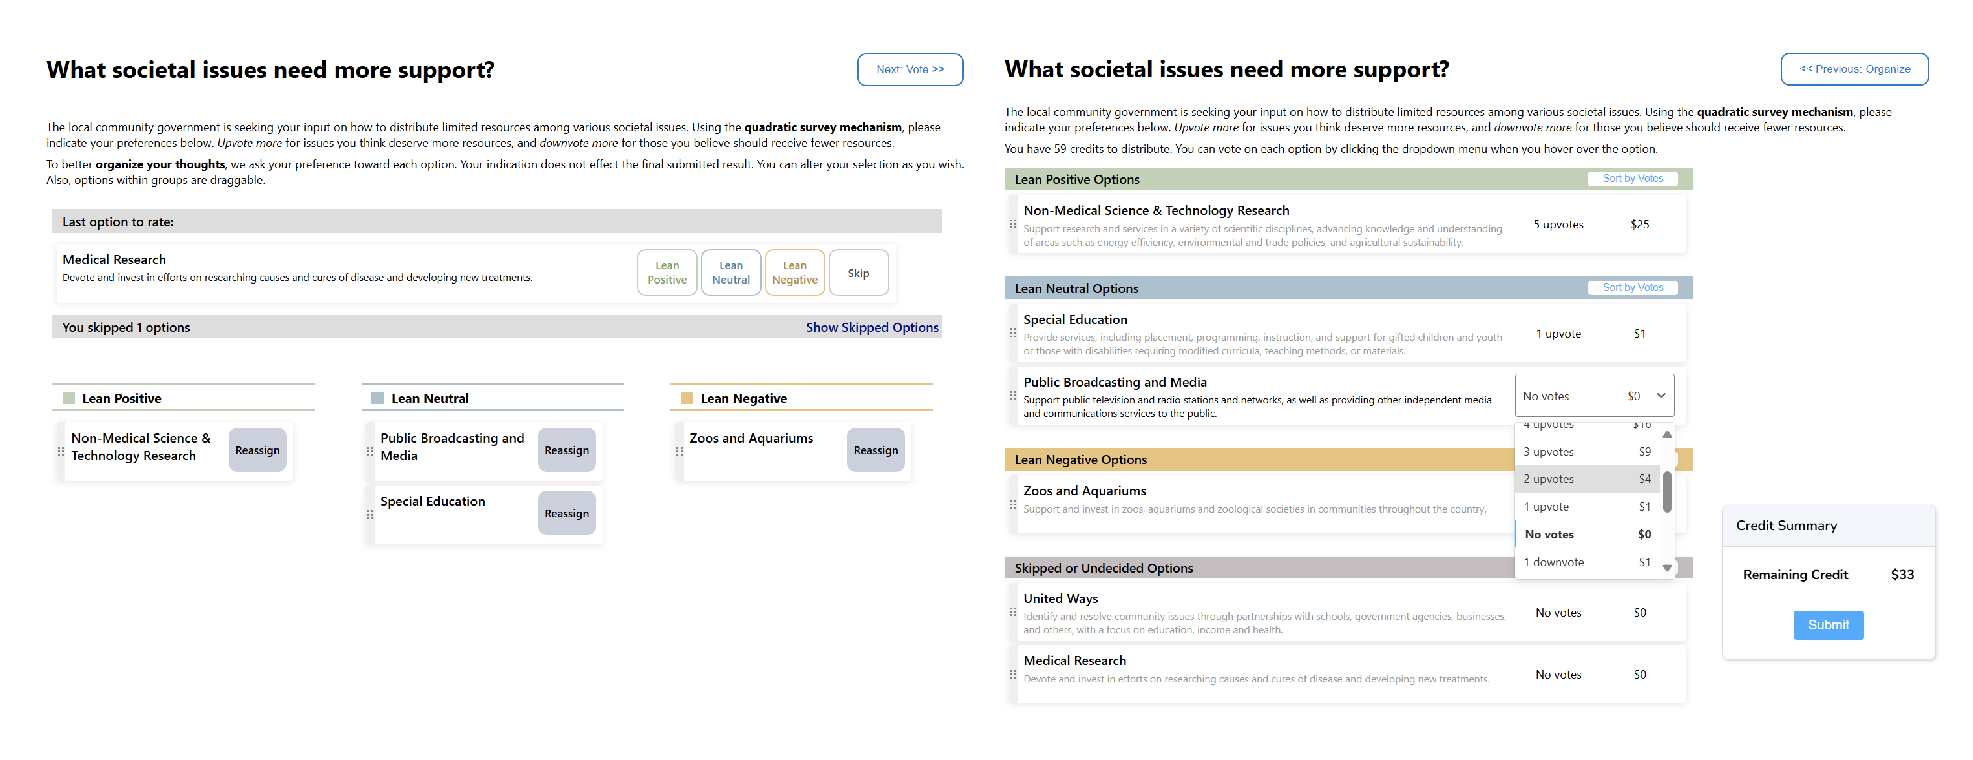
\includegraphics[width=\textwidth]{content/image/header.pdf}
%     \caption{A novel two-phase interactive interface for Quadratic Surveys detailed in Sec.~\ref{sec:finalInterfaceDesign}}
%     \label{fig:header}
% \end{figure}



% This challenge emphasizes the critical importance of designing and developing suitable interfaces for Quadratic Surveys to elicit truthful and in-depth preference information from respondents. Good design is essential; without it, the quality of collected data can suffer significantly. 
% These reasons strongly motivate  Addressing this question fills a important gap in the literature and enhances the practical utility of QS in capturing high-quality data across various applications.

% Highlight this is also the first work to investigate where people felt challenging when completing QS.
% At the same time, reducing cognitive load and making survey less challenging . Effective design may mitigate these overload challenges, ensuring that the Quadratic Survey mechanism fulfills its potential to capture detailed and accurate preferences. Thus, more concretely, this study focused on answering the following three research questions:

% 1. we design
% 2. we test across condition
% 3. understand what is difficult/hard through qualitative and quant responses
% --> design and usage recommendations

% Cited without details
% U.S. Colorado state government~\cite{rogersColoradoTriedNew2019}, the Democratic
%  Caucus of the House of Representatives~\cite{QuadraticVotingColorado} in the U.S., government-sponsored hackathons~\cite{teamTaiwanDigitalMinister}, and the recent Gov4git~\cite{Gov4gitDecentralizedPlatform2023}
% Despite the advocacy of Quadratic Voting by Posner and Weyl~\cite{posner2018radical}
% Political scientists have demonstrated that ballot designs alone can sway voter decisions~\cite{engstrom2020politics}, marketing and psychology researchers have examined how the presentation of questions influences responses~\cite{weijtersEffectRatingScale2010, kierujVariationsResponseStyle2010, toepoelSmileysStarsHearts2019}, and Human-Computer Interaction researchers have focused on evaluating and understanding web surveys and smart interfaces for surveys~\cite{farzandAestheticsEvaluatingResponse2024, xiaoTellMeYourself2020, pielotDidYouMisclick2024}. These studies highlight the importance of studying the interface and design for survey mechanisms.
% The Quadratic Mechanism is undeniably more complex than other voting and surveying mechanisms like the Likert scale survey~\cite{likertTechniqueMeasurementAttitudes1932}, where individuals select from a few responses, and Approval Voting~\cite{bramsApprovalVoting1978}, where participants mark as many options as they approve without constraints.

% Move this to related works.
% The effectiveness of eliciting these responses hinges upon the study protocol, survey mechanism, and design of the tool at hand~\cite{olsonWaysKnowingHCI2014, couperWebSurveyDesign2001, jackoHumancomputerInteractionHandbook2012}. While much research has explored the influence of the former two aspects, this research focuses on the design of a specific survey -- Quadratic Surveys. 

% Move this to discussion + contribution
% Thus, the primary goal of this study is to present a novel interactive interface designed for quadratic surveys, which could presumably extend to other applications that utilize the quadratic mechanism. 

% TODO, for a cleaner thesis statement in the first par? mention challenges and interface here before diving deeper.
% The importance of design in surveying tools, the growing usage of applications on the quadratic mechanism, and the lack of research on the design regarding quadratic mechanisms that one could apply, motivated our main research question: \textit{How can we design interactive interfaces to support participants in completing Quadratic Surveys?}

% Quadratic Surveys and other quadratic mechanism powered applications allow individuals 
% \begin{itemize}
% \item RQ1. How does the number of options on QS impact respondents' cognitive load?
% \item RQ2a. How does the interactive interface involving grouping and direct manipulation interface influence QS respondents' cognitive load compared to text-based interface?
% \item RQ2b. Across the two interfaces, what are the sources of cognitive load from?
% \item RQ3. What are differences in QS respondents' behaviors when coping with long lists of options?
% \end{itemize}

% Before answering these research questions, we iteratively designed and built an interactive interface informed by prior literature in the questionnaire and survey response format. Then, 
\section{Related Work}
\label{sec:relatedWorks}
This research lies at the intersection of three core areas:~\change{quadratic surveys, existing QV interfaces and choice overload along with cognitive challenges.} In this section, we review the related works in each of these areas.

% \afterpage{
% \clearpage
% \begin{figure}[p]
%     \centering
%     \begin{subfigure}[b]{1\textwidth}
%         \centering
%         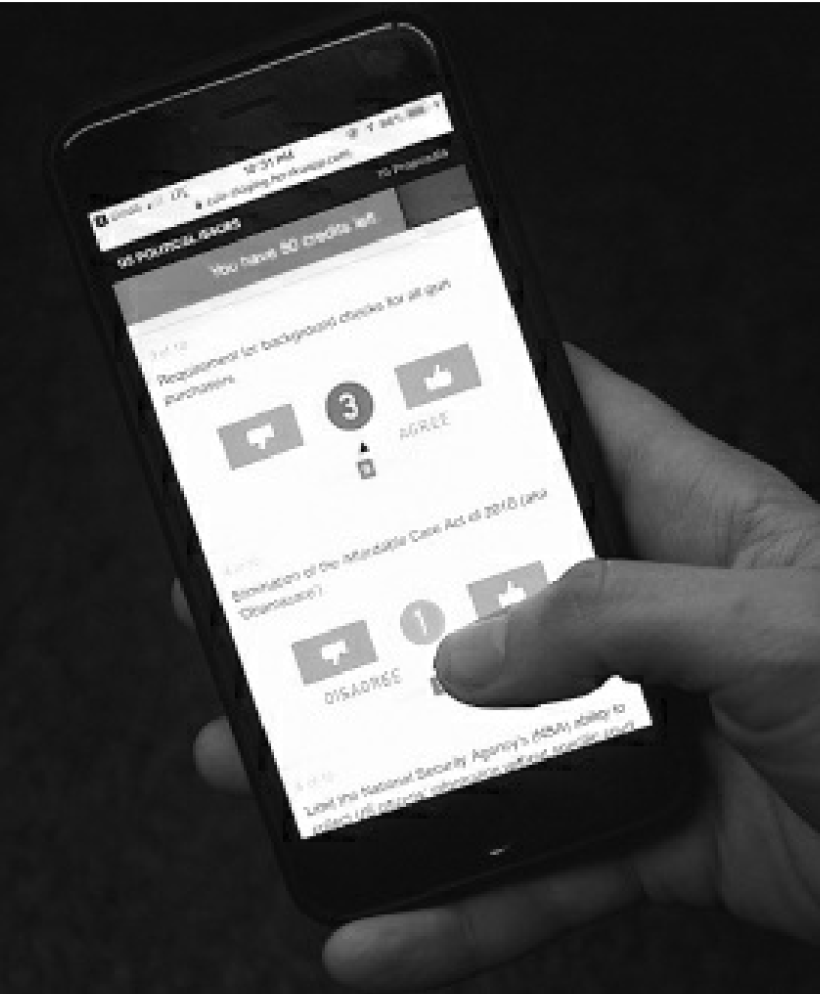
\includegraphics[width=0.4\textwidth]{content/image/curr_interface/radical_market_wedesign.png}
%         \caption{Software by WeDesign, used in the first empirical QV research~\cite{quarfoot2017quadratic}. Little information is available about the software, except for an image from~\textcite{posner2018radical}. In the image, each prompt has thumbs up and down icons to update the vote in the center. The remaining budget appears as a progress bar at the top.}
%         \Description{A black and white image of a mobile phone displaying a voting interface from software by WeDesign, used in empirical QV research. A hand holds the phone, and the screen shows a prompt related to background checks for gun purchases. There are thumbs-up and thumbs-down icons labeled "Agree" and "Disagree," with numbers indicating the current number of votes (e.g., 3 votes for "Agree"). A remaining vote budget is displayed at the top as a progress bar, indicating "50 choices left." The user is interacting with the interface, selecting either agree or disagree on the prompts.}
%         \label{fig:wedesignInterface}
%     \end{subfigure}

%     \vspace{1cm}

%     \begin{subfigure}[b]{1\textwidth}
%         \centering
%         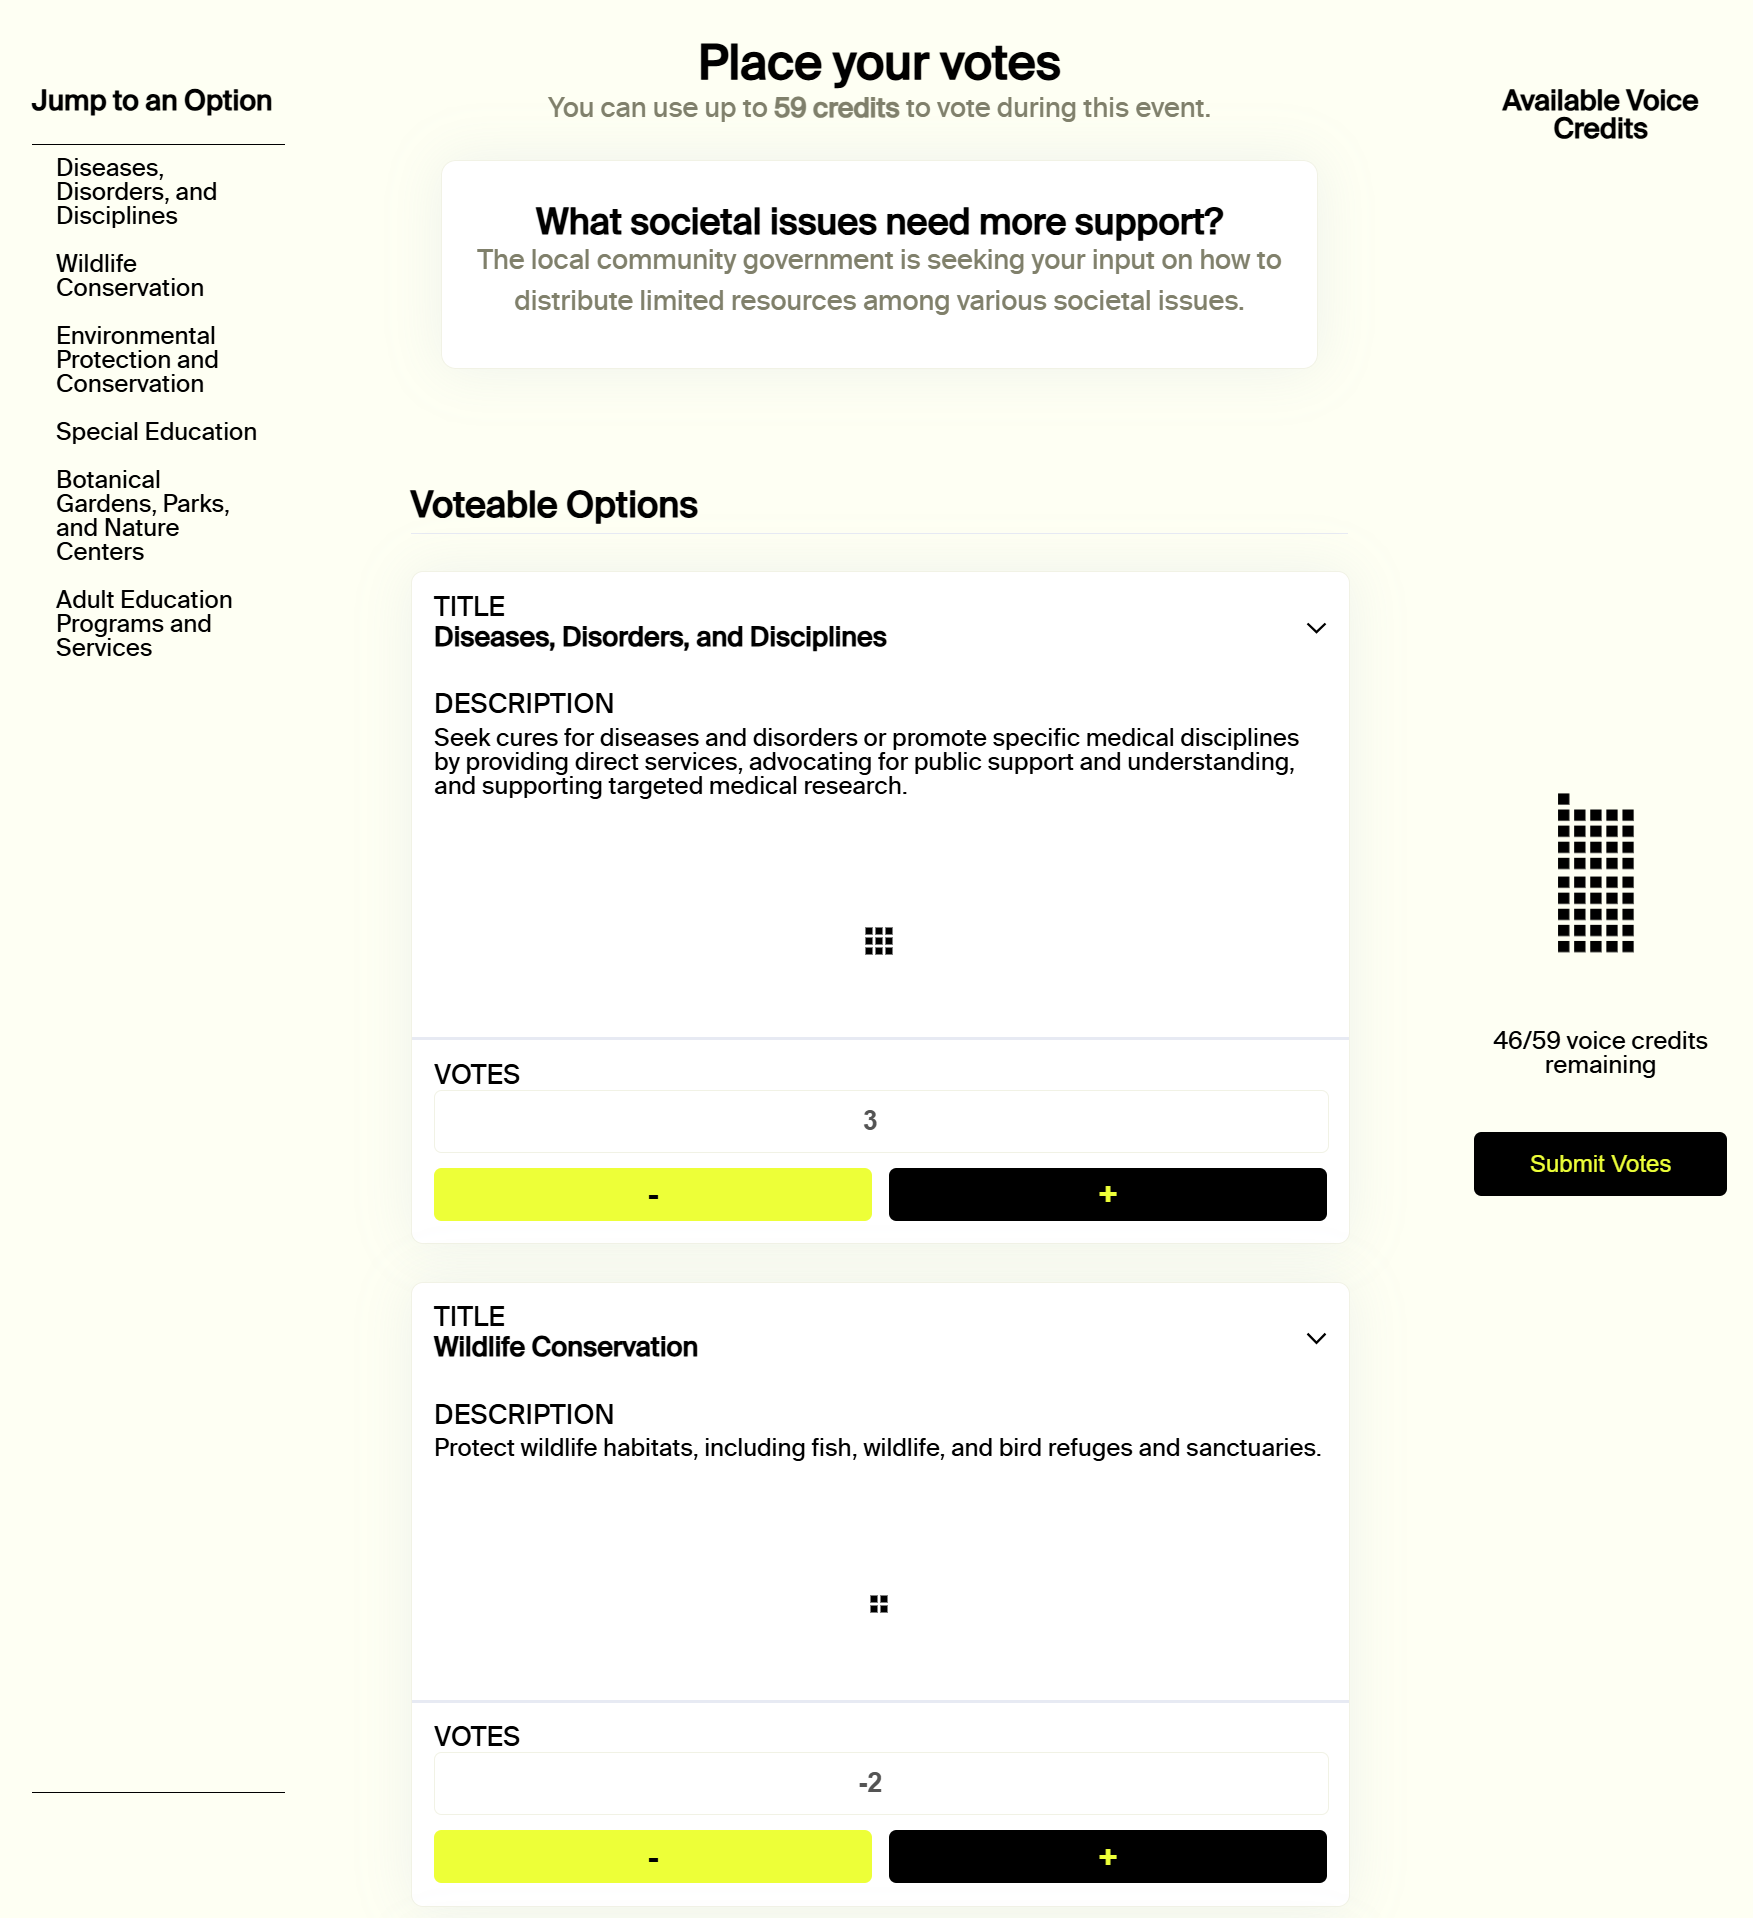
\includegraphics[width=0.5\textwidth]{content/image/curr_interface/rxc_interface.png}
%         \caption{An open-sourced QV interface~\cite{RadicalxChangeQuadraticvoting2024} forked from GitCoin~\cite{ReadWhitepaperGitcoin}, used by the RadicalxChange community~\cite{RxC}. This interface presents total credits as small blocks. Votes are updated using plus and minus buttons, with numerical counts shown under each option and surface area as costs.}
%         \Description{A screenshot of a Quadratic Voting (QV) interface designed for voting on societal issues that need more support. The screen displays two options: "Diseases, Disorders, and Disciplines" and "Wildlife Conservation," with a brief description under each. Users can adjust votes with plus and minus buttons, and the current vote count (e.g., 3 votes for Diseases, -2 votes for Wildlife Conservation) is displayed. The total available credits are shown on the right side as a grid of small blocks, with 46 out of 59 credits remaining. There is also a "Submit Votes" button. A menu on the left allows users to jump to different societal issues.}
%         \label{fig:rxcvotingInterface}
%     \end{subfigure}
    
%     % \vspace{0.12cm}
    
%     % \begin{subfigure}[b]{0.47\textwidth}
%     %     \centering
%     %     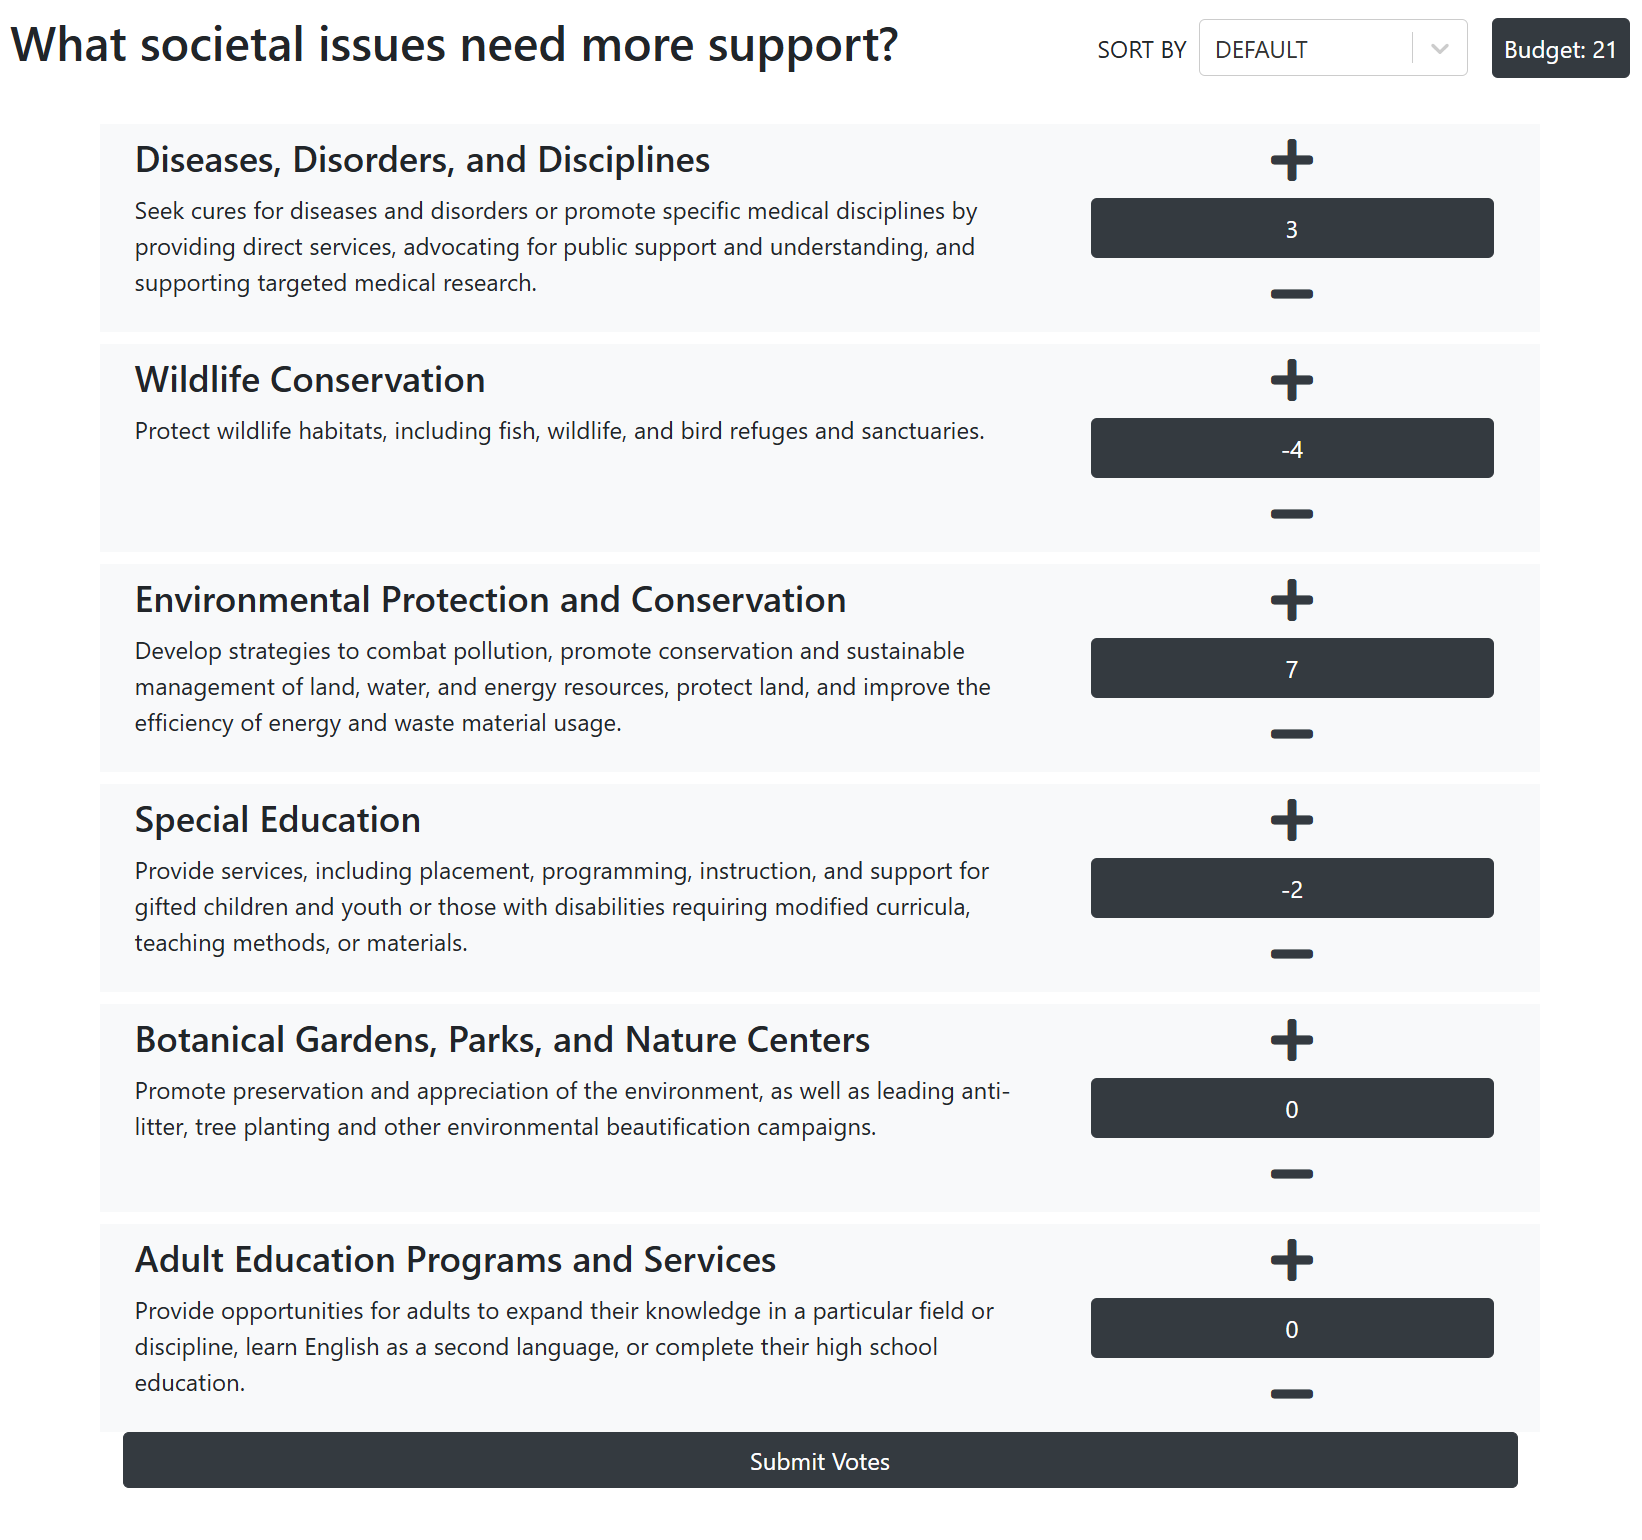
\includegraphics[width=0.72\textwidth]{content/image/curr_interface/geek.sg_interface.png}
%     %     \caption{An open-source QV interface~\cite{yehjxraymondYehjxraymondQvapp2024} offers a publicly available service. Options show only the current number of votes, with credits displayed in the top right corner. This interface does not show the costs of votes but supports sorting options.}
%     %     \Description{A screenshot of a Quadratic Voting (QV) interface for selecting societal issues that need more support. The interface presents six options: "Diseases, Disorders, and Disciplines," "Wildlife Conservation," "Environmental Protection and Conservation," "Special Education," "Botanical Gardens, Parks, and Nature Centers," and "Adult Education Programs and Services." Each option has a plus and minus button for allocating votes, with the current vote count displayed in a black box (e.g., 3 votes for "Diseases, Disorders, and Disciplines," -4 votes for "Wildlife Conservation," and 7 votes for "Environmental Protection and Conservation"). The budget of 21 credits is shown at the top right of the interface, and there is a "Submit Votes" button at the bottom. The interface also includes a sorting option set to "Default," though no vote cost information is displayed.}
%     %     \label{fig:yehInterface}
%     % \end{subfigure}
%     % \hspace{0.4cm}
%     % \begin{subfigure}[b]{0.47\textwidth}
%     %     \centering
%     %     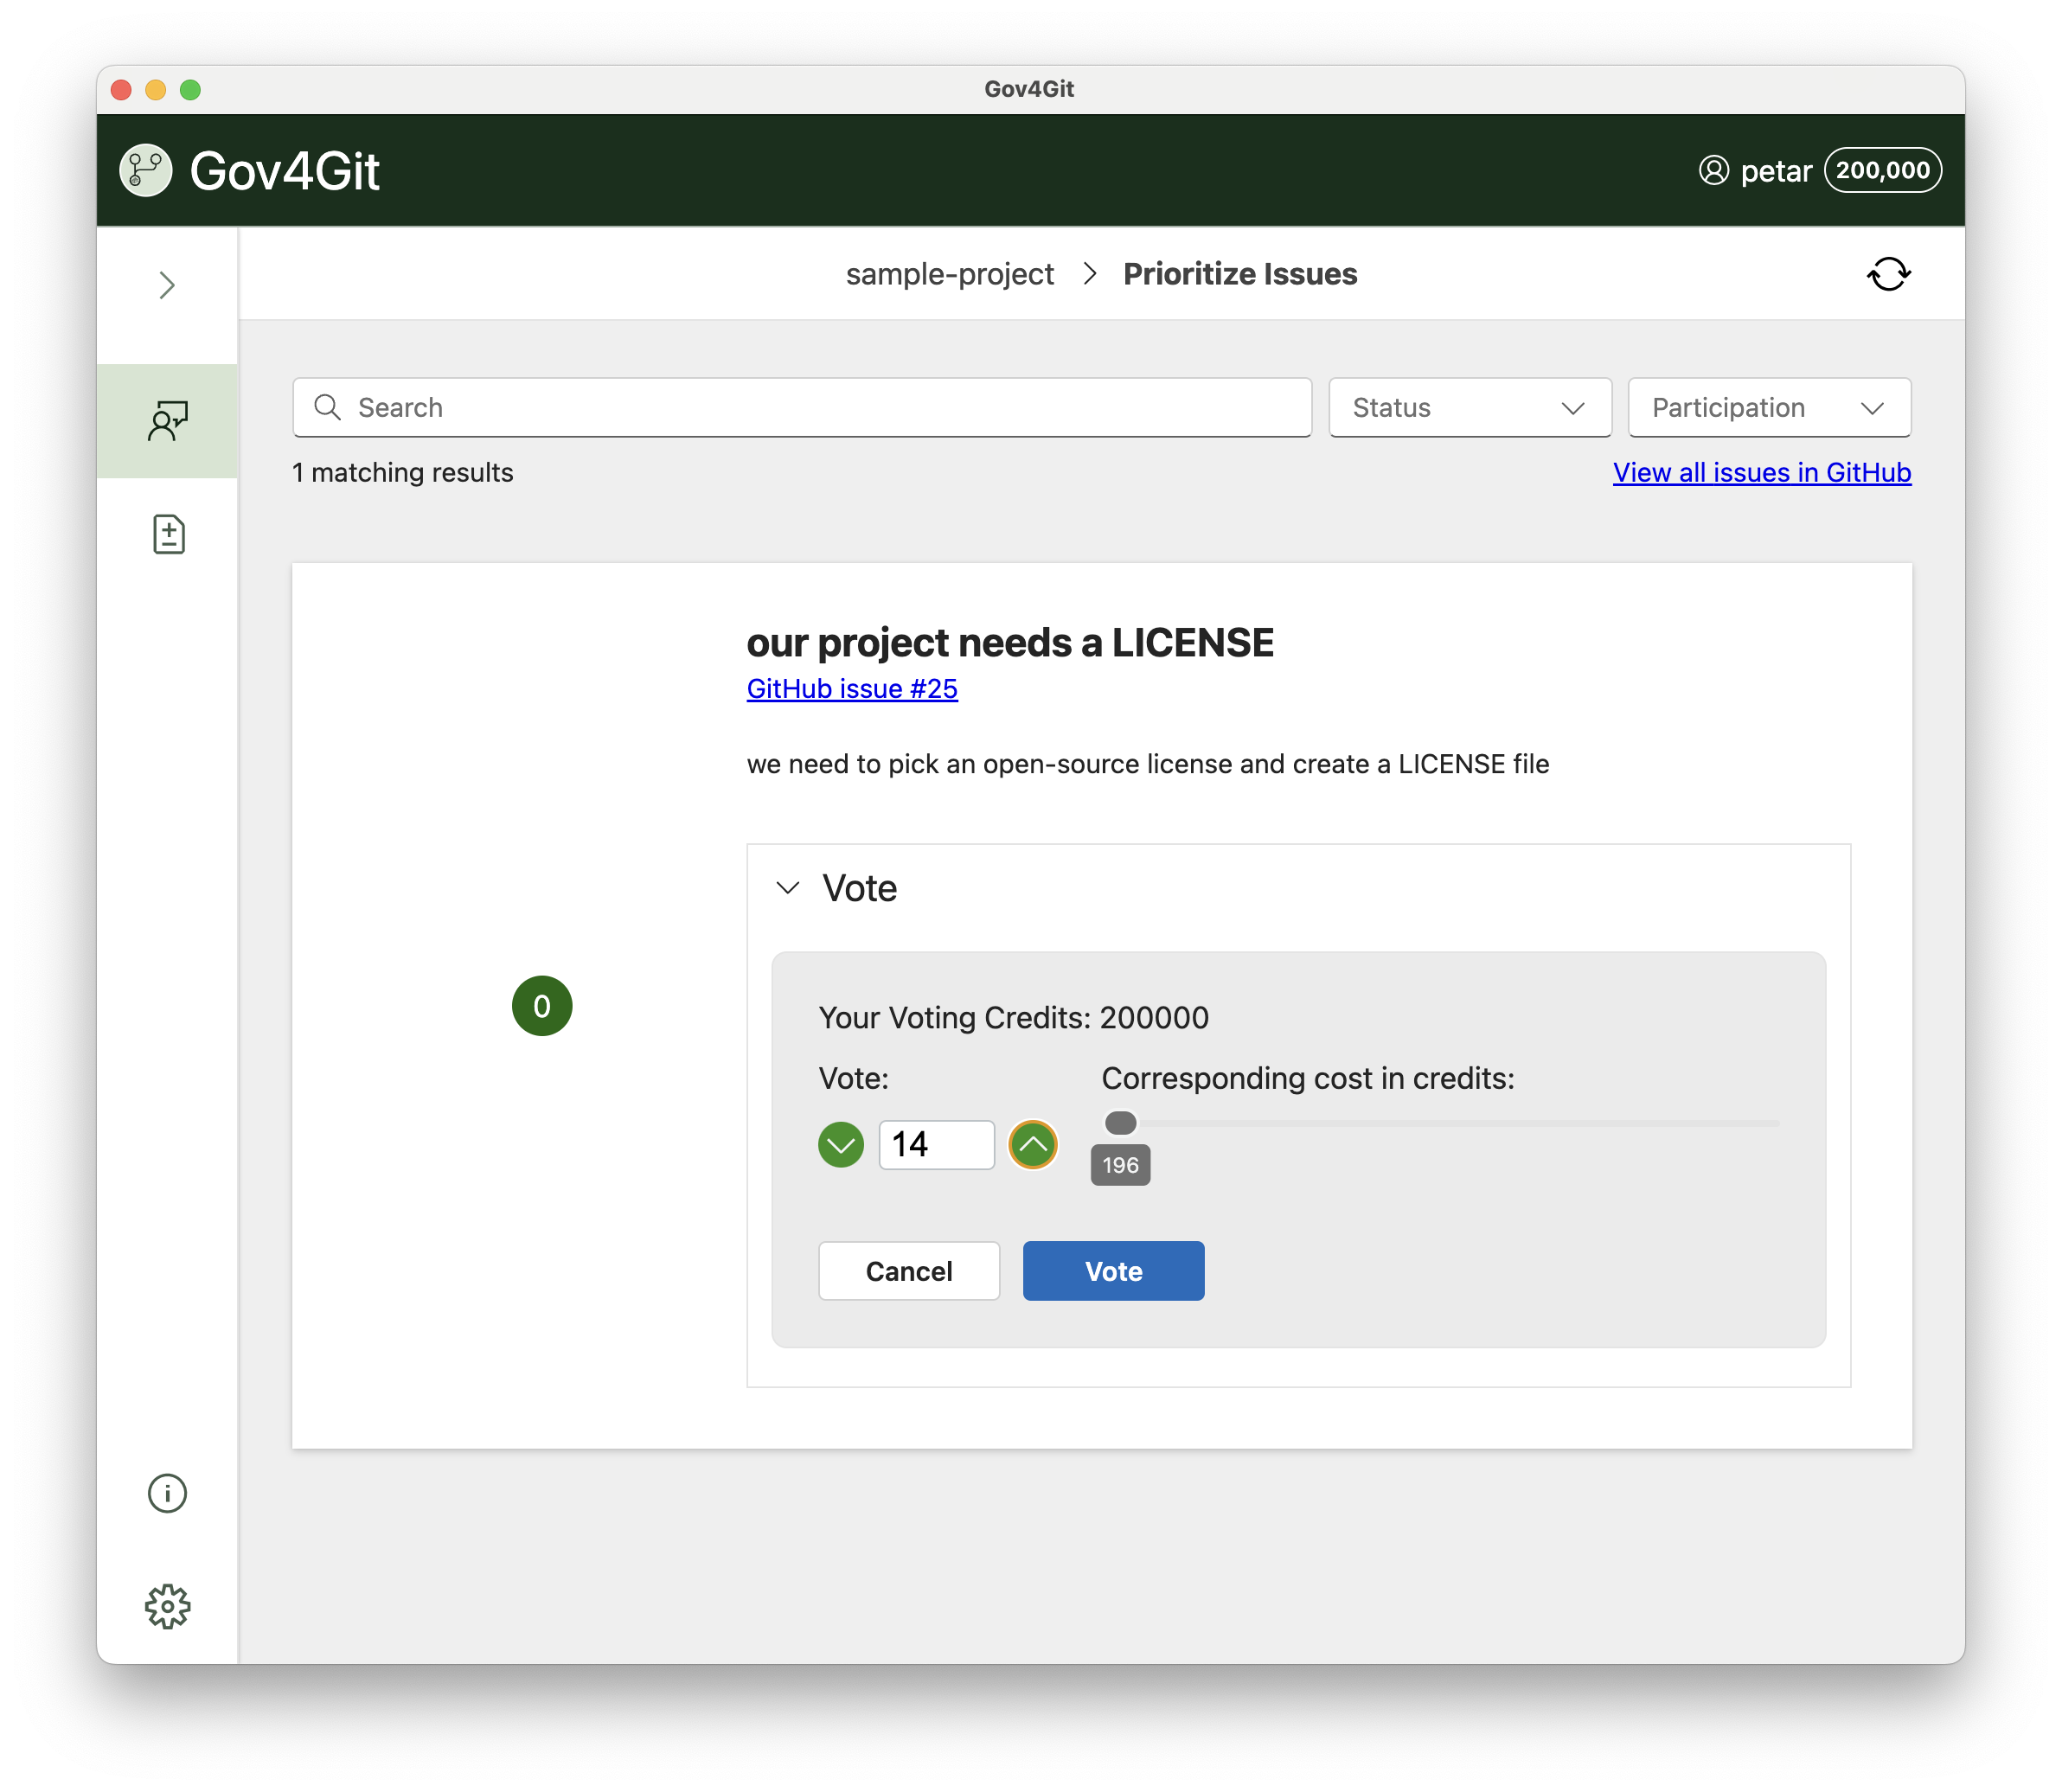
\includegraphics[width=0.72\textwidth]{content/image/curr_interface/appvote.png}
%     %     \caption{The interface designed for gov4git~\cite{Gov4gitDecentralizedPlatform2023} updates votes using arrows under each option, with the associated cost shown as a percentage bar to the right. A search bar exists for searching specific pull requests or issues.}
%     %     \Description{The screenshot displays the interface of the Gov4Git application on a desktop browser. At the top left, the Gov4Git logo and the project name "sample-project" are shown, with a breadcrumb navigation bar leading to "Prioritize Issues." Below, the main section shows an issue titled "our project needs a LICENSE," linked to a corresponding GitHub issue \#25. The text suggests that the team needs to select an open-source license. Below the issue description is a "Vote" box displaying available voting credits (200,000) and options to vote with a green up-arrow. The user has entered a vote of 14, with a corresponding cost of 196 credits shown next to the percentage bar. Options to cancel or submit the vote are shown at the bottom. The interface includes a search bar and drop-down filters for status and participation. The user is identified at the top right as "petar" with 200,000 credits.}
%     %     \label{fig:gov4gitInterface}
%     % \end{subfigure}
    
%     % \vspace{0.15cm}
    
%     % \begin{subfigure}[b]{0.7\textwidth}
%     %     \centering
%     %     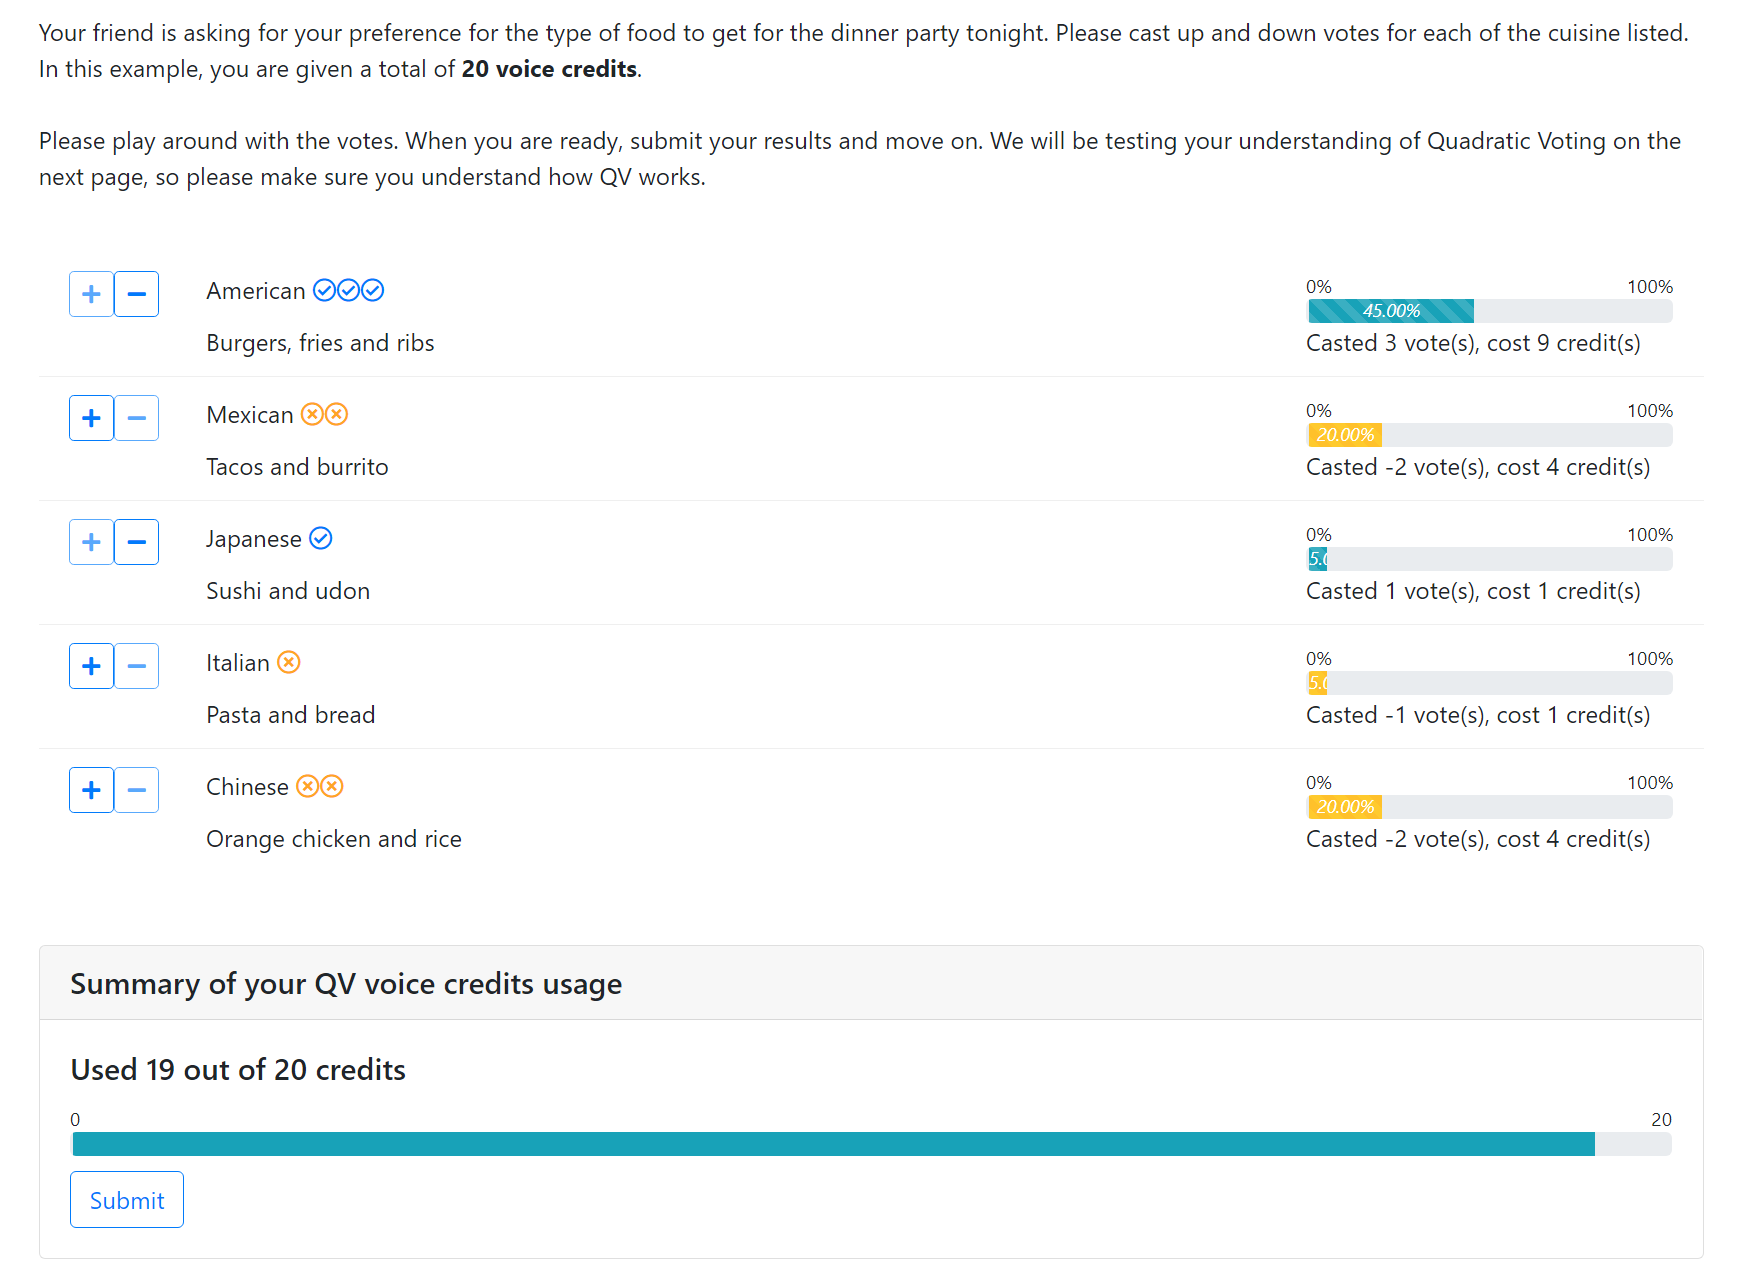
\includegraphics[width=0.50\textwidth]{content/image/curr_interface/cheng_qv.png}
%     %     \caption{The interface used in the research by~\textcite{chengCanShowWhat2021} employs the most visual components. Icons depict the current number of votes, with progress bars signifying the current spending.}
%     %     \Description{A screenshot of a Quadratic Voting (QV) interface, where users are asked to allocate 20 voice credits to vote on preferred food options for a dinner party. The interface presents five cuisine options: American (burgers, fries, and ribs), Mexican (tacos and burritos), Japanese (sushi and udon), Italian (pasta and bread), and Chinese (orange chicken and rice). Each option has plus and minus buttons to increase or decrease votes, along with icons displaying the number of votes placed. A progress bar beside each cuisine shows the percentage of votes cast, and corresponding text details the number of votes and credits used (e.g., 3 votes for American costing 9 credits). Below the voting section, a summary bar shows the total of 19 out of 20 credits used, with a "Submit" button at the bottom of the page.}
%     %     \label{fig:chengInterface}
%     % \end{subfigure}
    
%     \caption{Recent interface for applications using the quadratic mechanism.}
%     \Description{A collection of 5 interfaces showcasing various interfaces.}
%     \label{fig:qv_interface_external}
% \end{figure}
% \clearpage
% }
\begin{figure}[h]
    \centering
    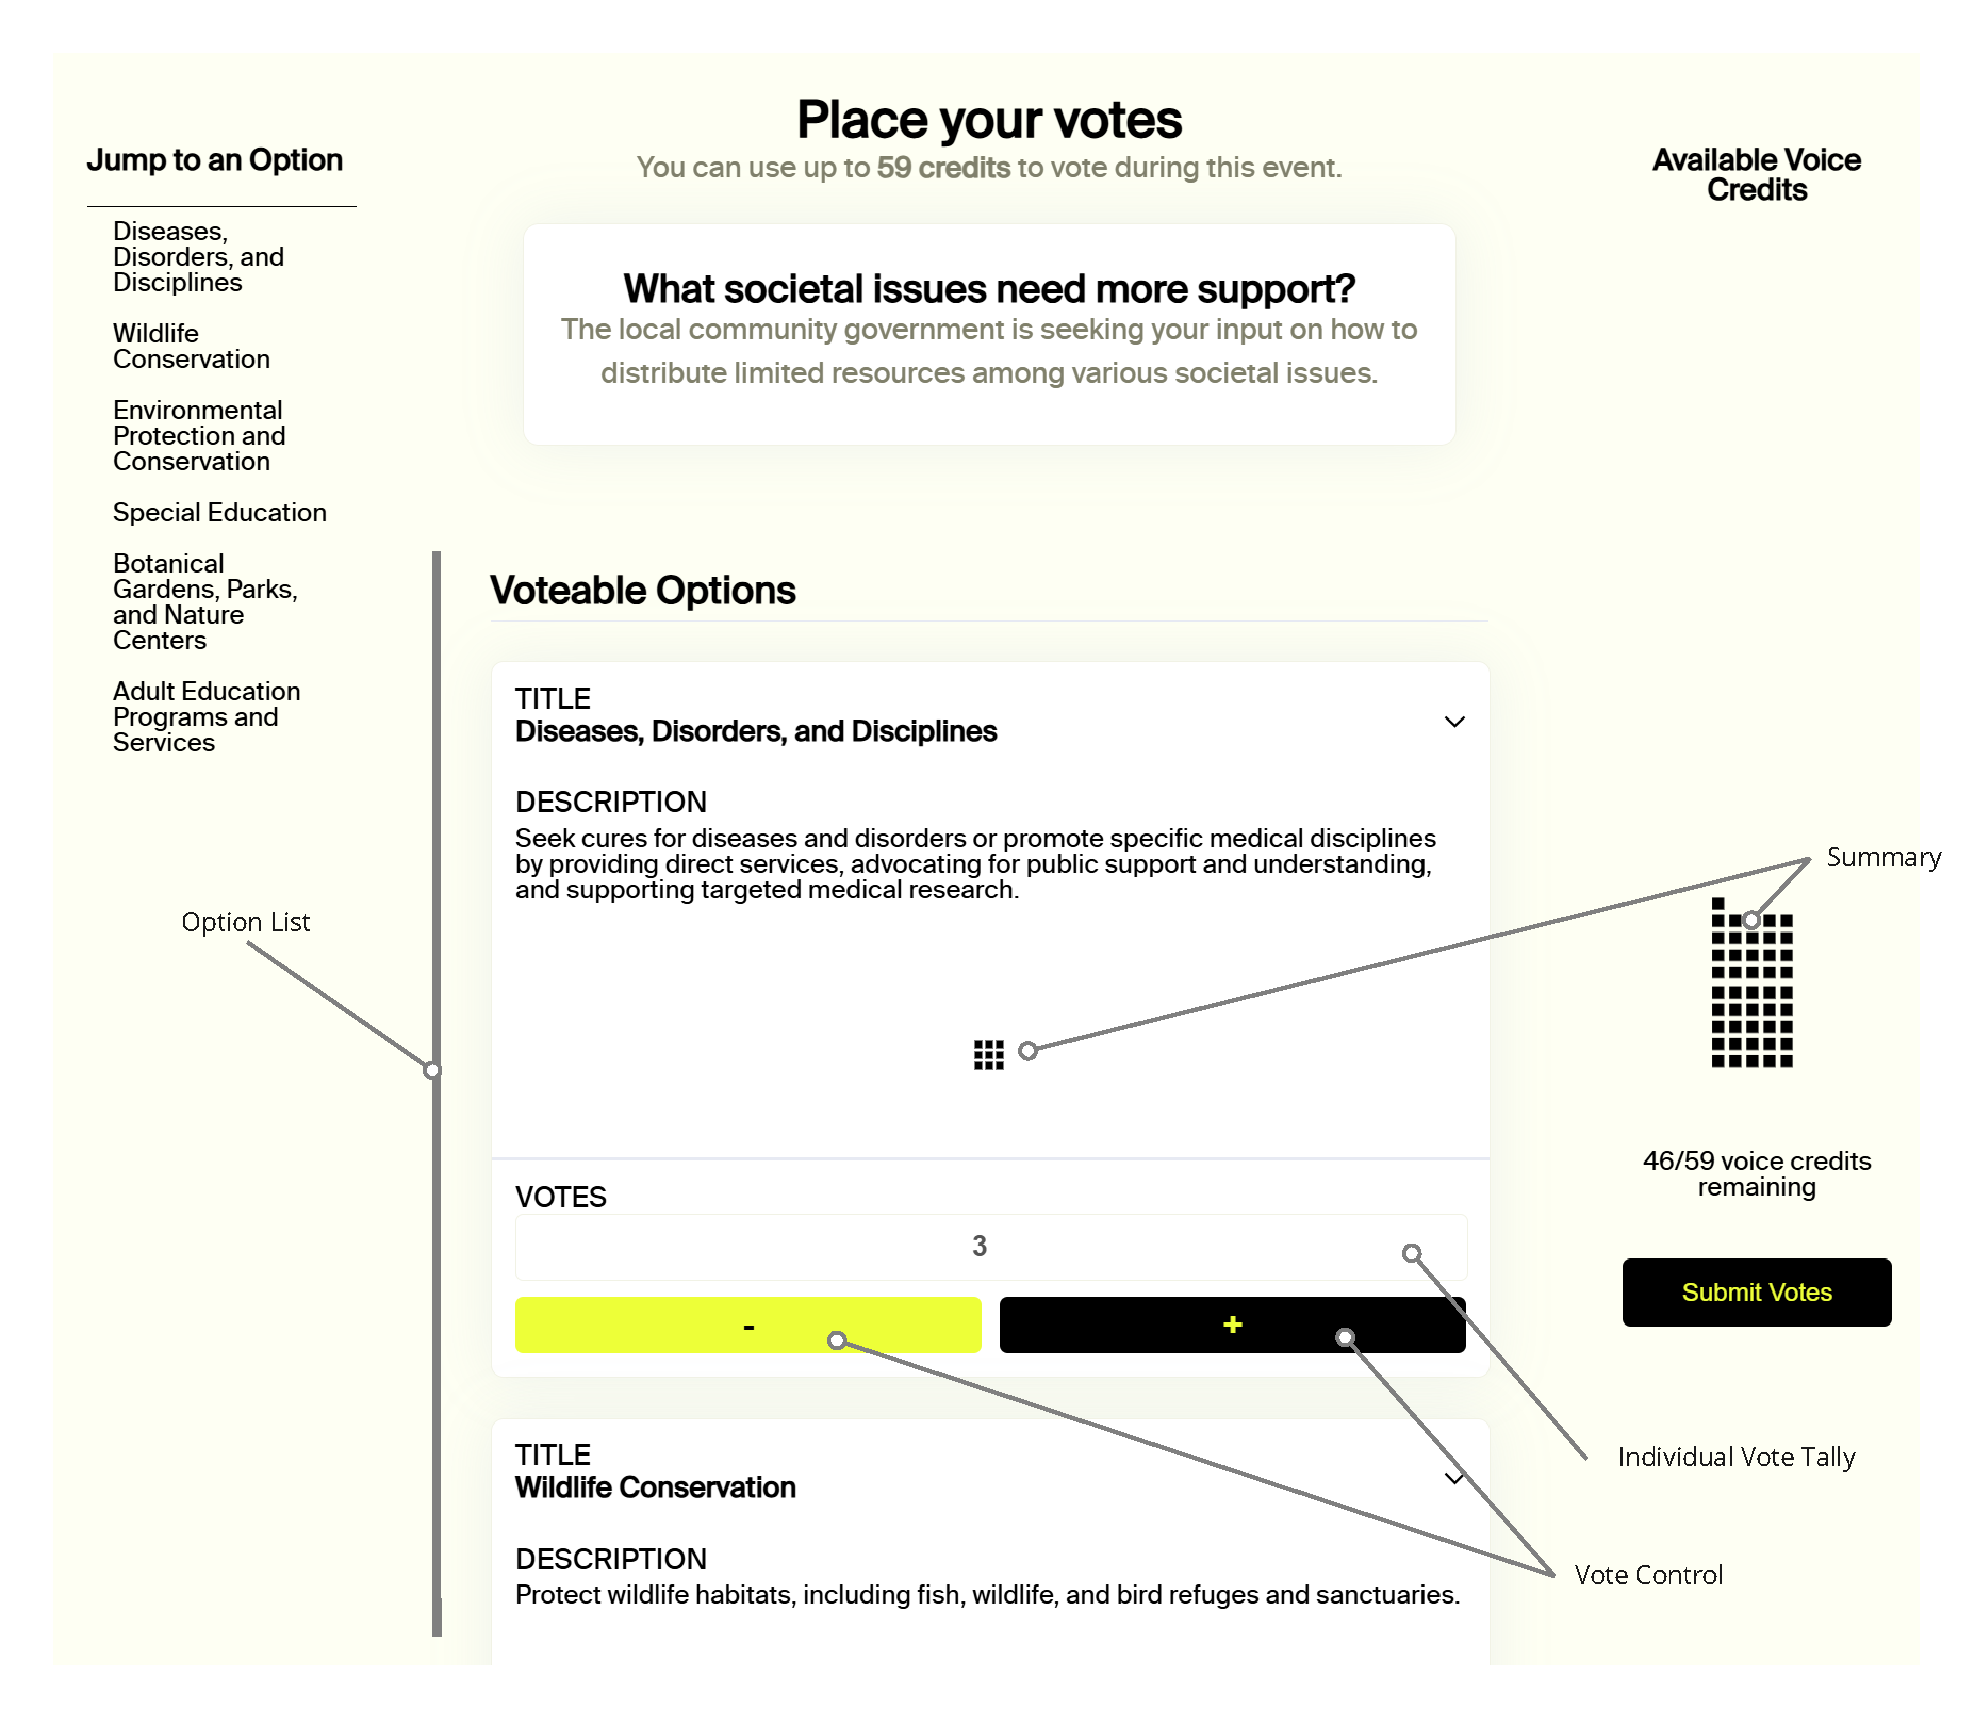
\includegraphics[width=0.7\textwidth]{content/image/curr_interface/rxc_interface_annotated.pdf}
    \caption{An open-sourced QV interface~\cite{RadicalxChangeQuadraticvoting2024} forked from GitCoin~\cite{ReadWhitepaperGitcoin}, used by the RadicalxChange community~\cite{RxC}. Votes are updated through plus and minus buttons, with numerical vote tallying under each option. This interface used small blocks to represent remaining credits and individual option costs.}
    \Description{}
    \label{fig:rcx_interface_annotated}
\end{figure}

\begin{figure}[h]
    \centering
    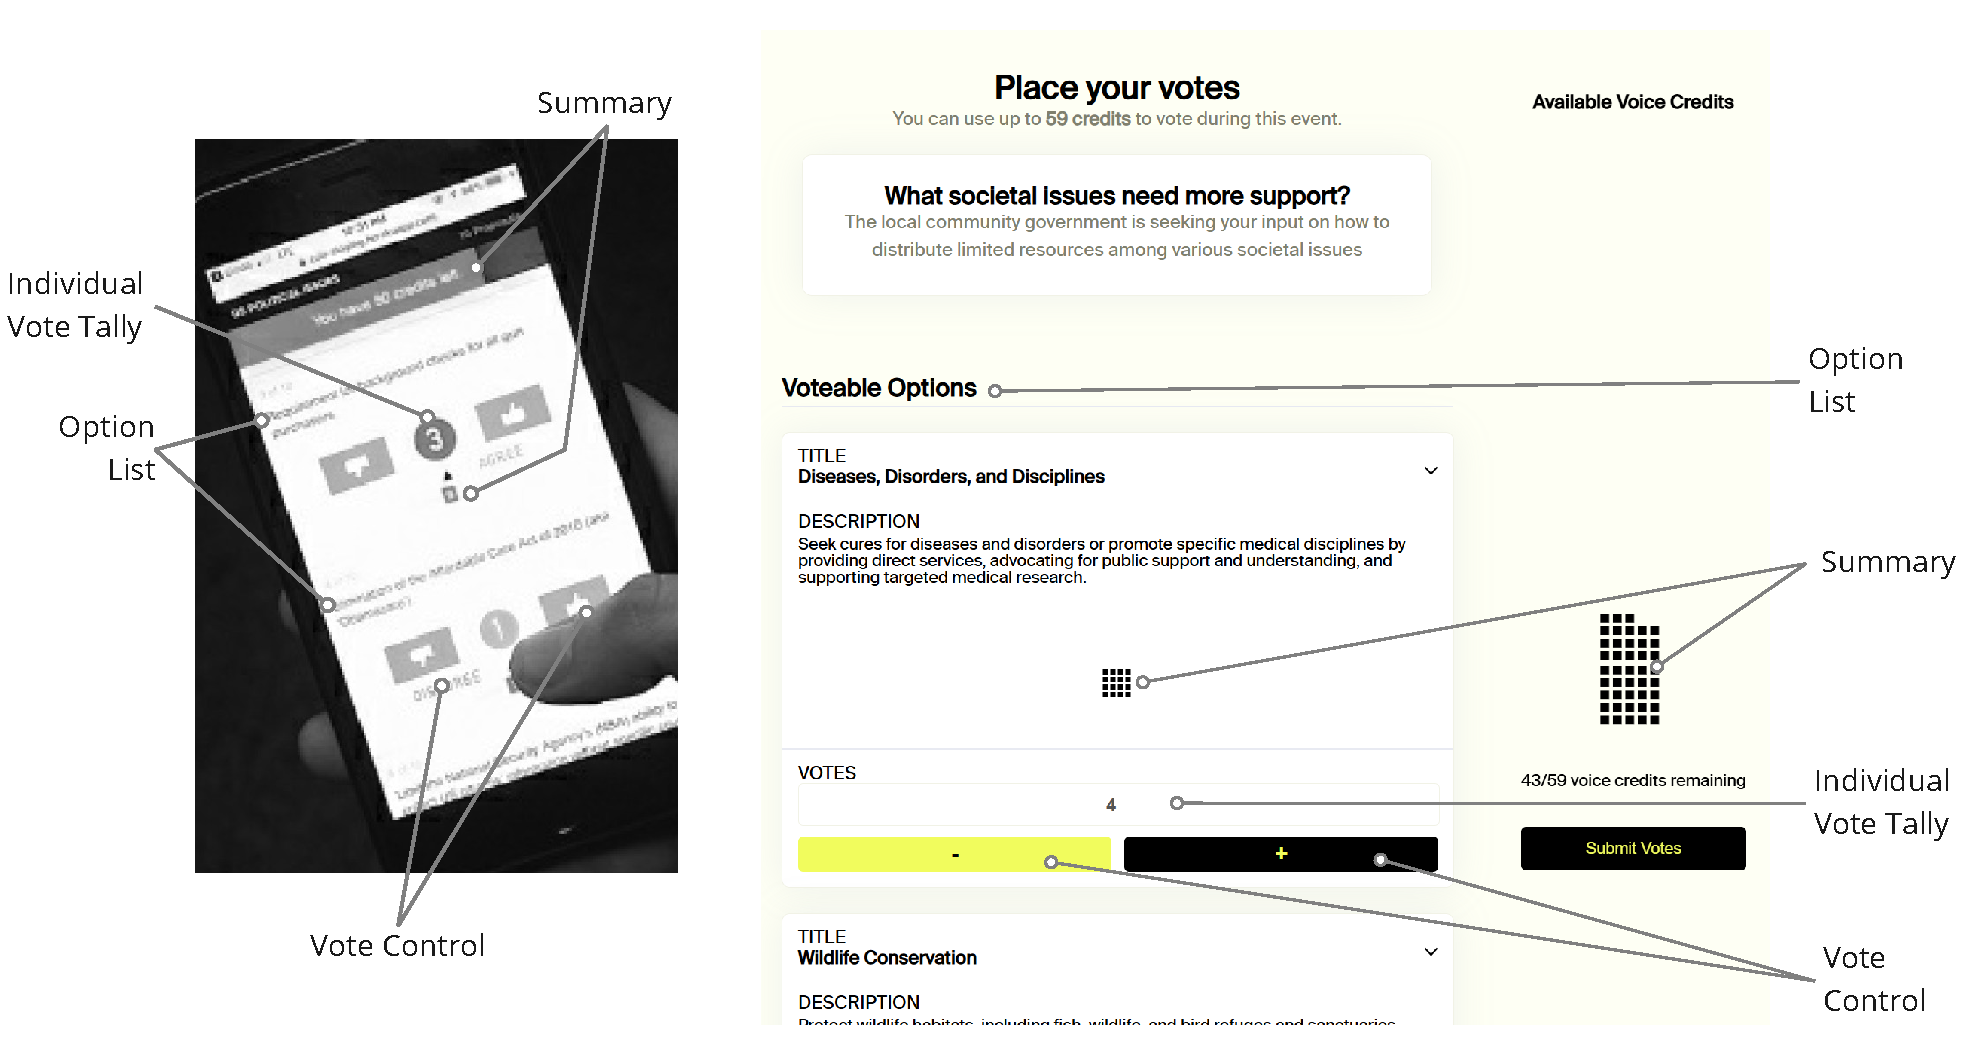
\includegraphics[width=\textwidth]{content/image/curr_interface/recent_annotated.pdf}
    \caption{An open-sourced QV interface~\cite{RadicalxChangeQuadraticvoting2024} forked from GitCoin~\cite{ReadWhitepaperGitcoin}, used by the RadicalxChange community~\cite{RxC}. Votes are updated through plus and minus buttons, with numerical vote tallying under each option. This interface used small blocks to represent remaining credits and individual option costs.}
    \Description{}
    \label{fig:rcx_interface_annotated}
\end{figure}

%     \begin{subfigure}[b]{1\textwidth}
%         \centering
%         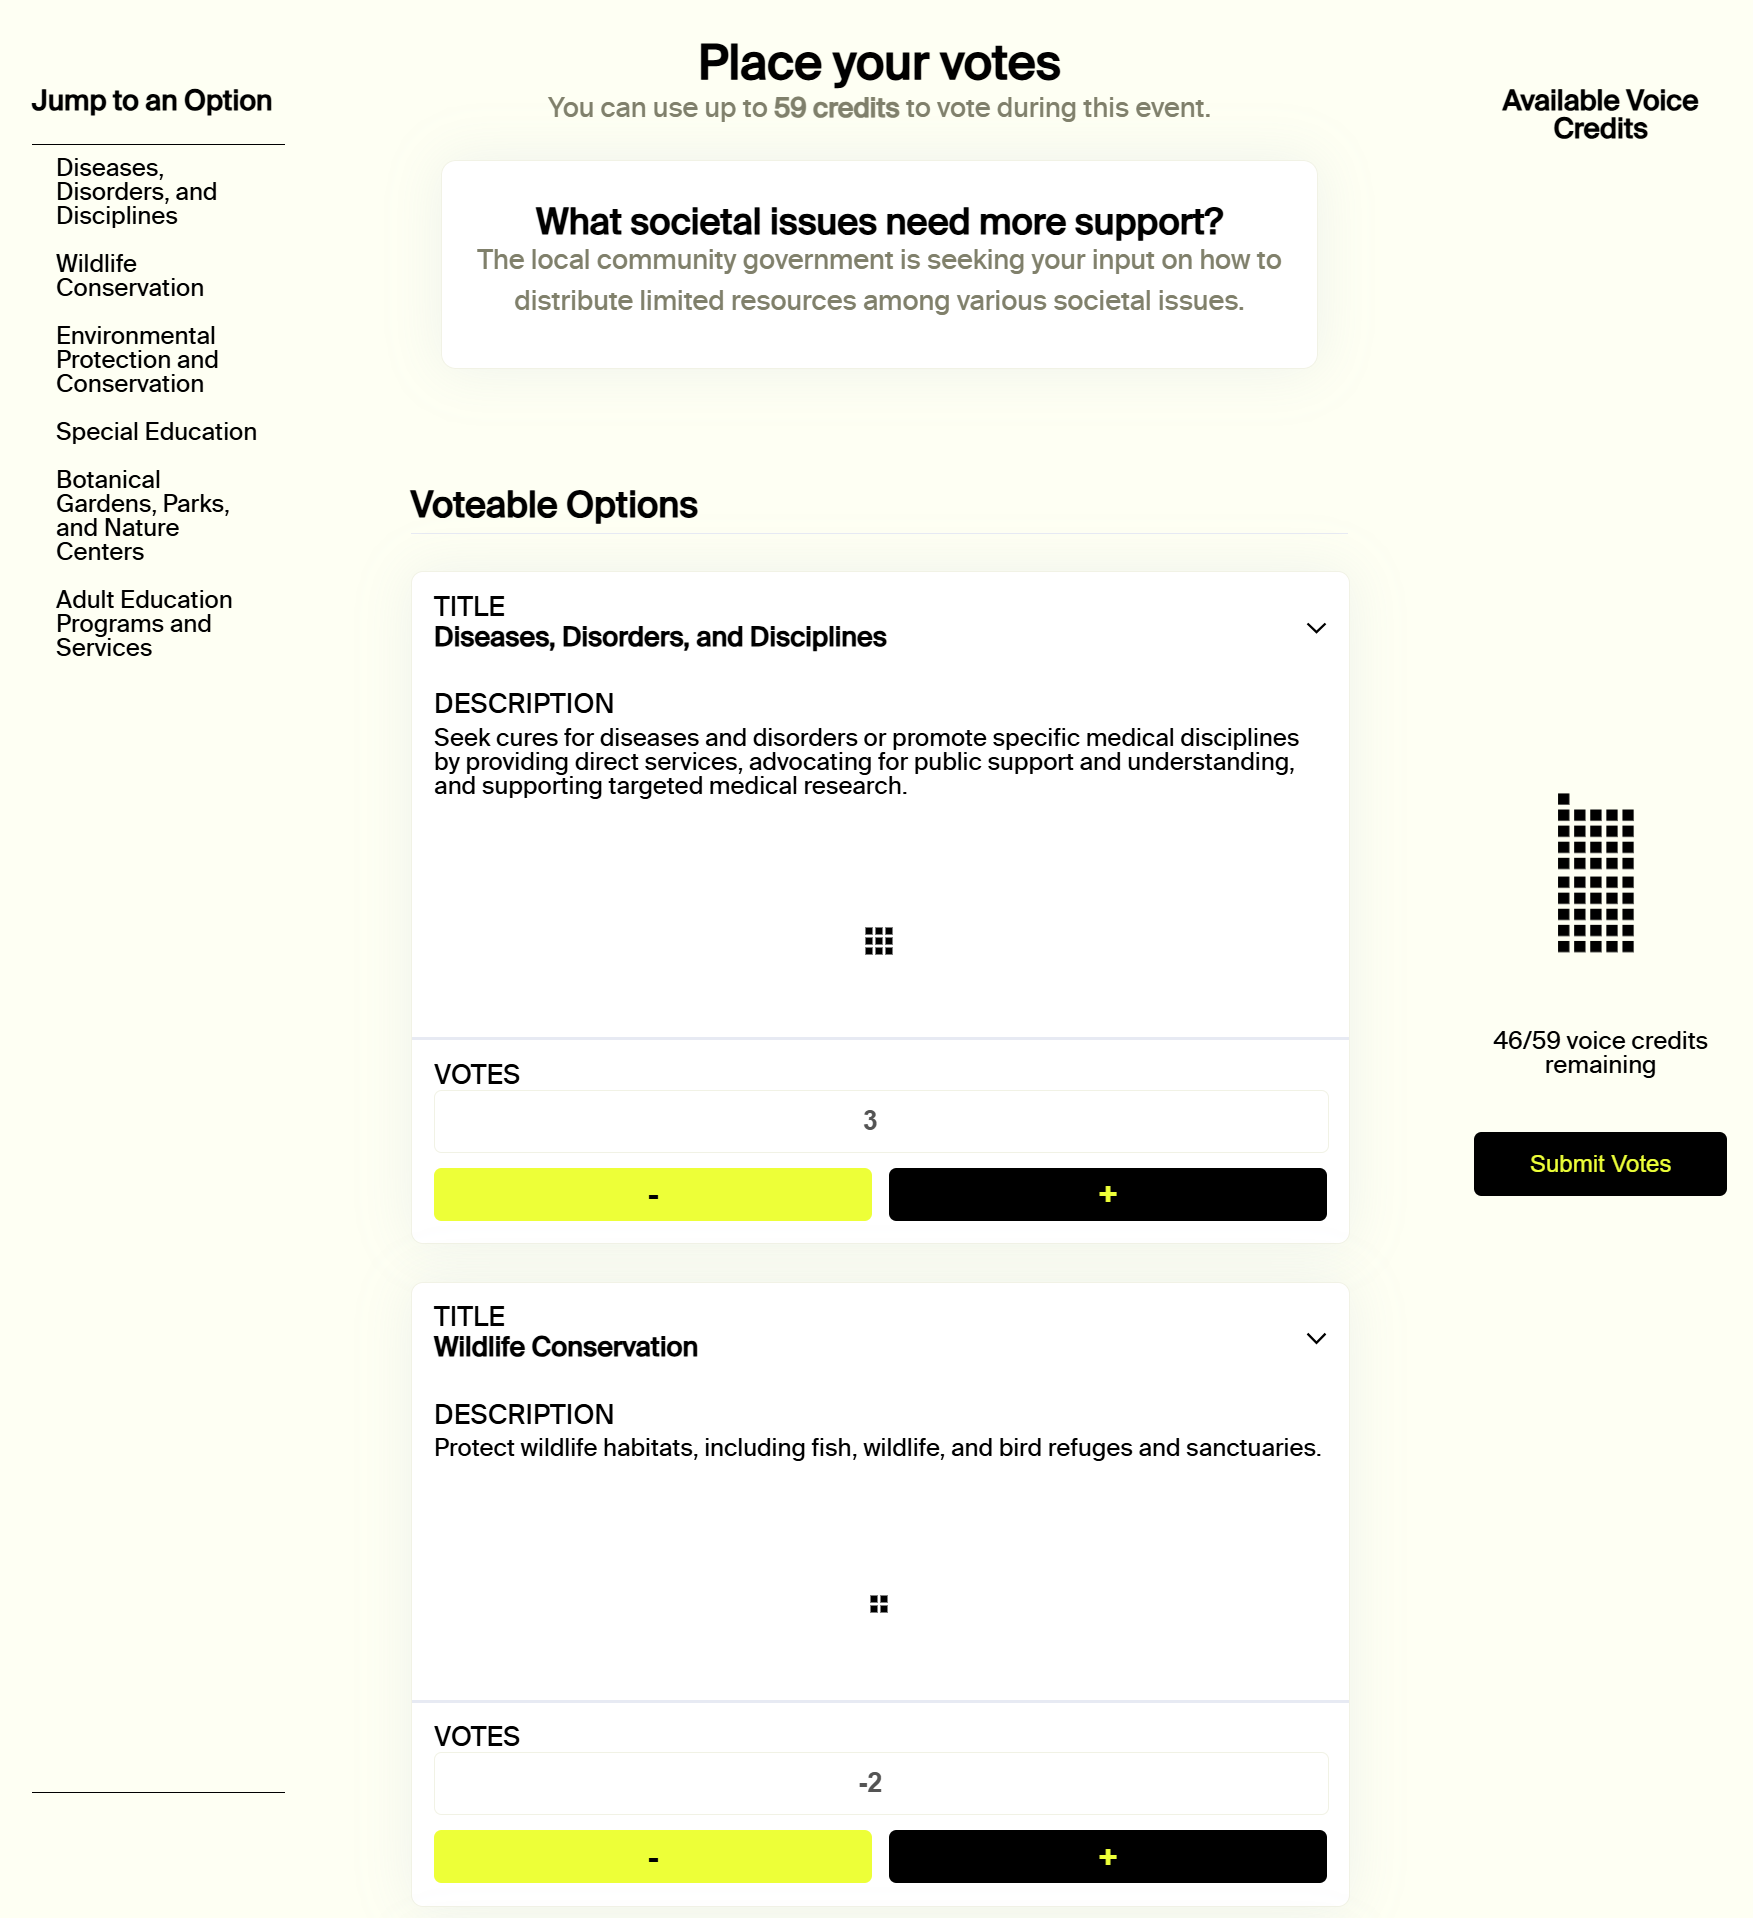
\includegraphics[width=0.5\textwidth]{content/image/curr_interface/rxc_interface.png}
%         \caption{An open-sourced QV interface~\cite{RadicalxChangeQuadraticvoting2024} forked from GitCoin~\cite{ReadWhitepaperGitcoin}, used by the RadicalxChange community~\cite{RxC}. This interface presents total credits as small blocks. Votes are updated using plus and minus buttons, with numerical counts shown under each option and surface area as costs.}
%         \Description{A screenshot of a Quadratic Voting (QV) interface designed for voting on societal issues that need more support. The screen displays two options: "Diseases, Disorders, and Disciplines" and "Wildlife Conservation," with a brief description under each. Users can adjust votes with plus and minus buttons, and the current vote count (e.g., 3 votes for Diseases, -2 votes for Wildlife Conservation) is displayed. The total available credits are shown on the right side as a grid of small blocks, with 46 out of 59 credits remaining. There is also a "Submit Votes" button. A menu on the left allows users to jump to different societal issues.}



\subsection{Quadratic Survey and the Quadratic Mechanism}
We introduce the term \textbf{Quadratic Survey (QS)} to describe surveys that utilize the quadratic mechanism to collect individual attitudes. The~\textbf{quadratic mechanism} is a theoretical framework designed to encourage the truthful revelation of individual preferences through a quadratic cost function~\cite{grovesOptimalAllocationPublic1977}. This framework gained popularity through~\textbf{Quadratic Voting (QV)}, also known as plural voting, which uses a quadratic cost function in a voting framework to facilitate collective decision-making~\cite{lalley2016quadratic}.

To illustrate how QS works, we formally define the mechanism: each survey respondent is allocated a fixed budget, denoted by $B$, to distribute among various options. Participants can cast $n$ votes for or against option~$k$. The cost~$c_k$ for each option $k$ is derived as:
\begin{equation*}
c_k = n_k^2 \quad \text{where}\quad n_k \in \mathbb{Z}
\end{equation*}
The cost of all votes must not exceed the participant's budget:
\begin{equation*}
\sum_k c_k \leq B
\end{equation*}
Survey results are determined by summing votes for each option:
\begin{equation*}
\text{Total Votes for Option } k = \sum_{i=1}^{S} n_{i,k}    
\end{equation*}
where $S$ represents the total number of participants, and~$n_{i,k}$ is the number of votes cast by participant~$i$ for option~$k$. Each additional vote for each option increases the marginal cost linearly, encouraging participants to vote proportionally to their level of concern for an issue~\cite{posner2018radical}.

QS adapts these strengths of the quadratic mechanism in \textit{voting} to encourage truthful expression of preferences in \textit{surveys}. Unlike traditional surveys that elicit either rankings~\textit{or} ratings, QS allows for~\textit{both}, enabling participants to cast multiple votes for or against options, incurring a quadratic cost.~\citet{chengCanShowWhat2021} showed that this mechanism aligns individual preferences with behaviors more accurately than Likert Scale surveys, particularly in resource-constrained scenarios like prioritizing user feedback on user experiences.

In recent years, empirical studies on QV have expanded into various domains~\cite{naylor2017first, cavaille2024cares}. Applications based on the quadratic mechanism have also grown, including Quadratic Funding, which redistributes funds based on outcomes from consensus made using the quadratic mechanism~\cite{buterinFlexibleDesignFunding2019a, freitasQuadraticFundingIncomplete2024}. Recent work by \citet{southPluralManagement2024} applies the quadratic mechanism to networked authority management, later used in Gov4git~\cite{Gov4gitDecentralizedPlatform2023}. Despite the increasing breadth and depth of applications utilizing the quadratic mechanism, little attention has been paid to user experience and interface design, which support individuals' preference intensity elicitation. Our work aims to address this by designing interfaces for quadratic mechanisms.

\subsection{Existing QV Interfaces}
\label{sec:related_qv}

Since QS shares QV's underlying mechanism, we used snowball sampling to identify publicly available QV applications mentioned in news and academic sources. Currently, no widely adopted QV interface is tied to a single vendor or platform.~\Cref{fig:rcx_interface_annotated} shows two variations of existing QV interfaces, with both employing a single-step approach with different visual representations of common elements~\cite{Gov4gitDecentralizedPlatform2023, yehjxraymondYehjxraymondQvapp2024, chengCanShowWhat2021, cavaille2024cares}. All QV interfaces generally include:

\begin{itemize}[leftmargin=*]
    \item Option list: A list of options for voting.
    \item Vote controls: Buttons to add or remove votes for each option.
    \item Individual vote tally: A display of the votes cast per option.
    \item Summary: A summary of costs and the remaining budget.
\end{itemize}

These components let users operate QV mechanically, providing little understanding of voters' usability needs nor offering cognitive support. In addition, HCI research on survey interfaces is limited~\cite{nobarany2012design, van2007design} with most efforts focusing on alternative input modalities like bots, voice interfaces, or virtual reality~\cite{voiceWei2022, khullar2021, kimComparingDataChatbot2019, feick2020virtual}.

\subsection{Cognitive Challenges and Choice Overload}
The challenge of respondents making difficult decisions using quadratic mechanisms remains unexplored in the literature.~\citet{lichtensteinConstructionPreference2006} identified three key elements that make decisions difficult. \change{These elements include making decisions in unfamiliar contexts, quantifying the value of one's opinions, and being forced to make trade-offs due to conflicting choices. QS fits at least two of the three elements: participants may encounter a selection of unfamiliar options by the survey designer; they are asked to quantify the difference between option preferences through a numerical vote; and the budget constraint enforces trade-offs under a non-linear function, which means that a vote decrease for one option is not necessary equivalent to an increase for another, making iterative adjustment and evaluating tradeoffs difficult. Thus, we believe QS introduces a high cognitive load.}

Cognitive load refers to the demands placed on a user's working memory during the interaction process, which significantly influences the usability of the system~\cite{cooper1998research, seppCognitiveLoadTheory2019}. Cognitive overload can adversely affect performance~\cite{drommi2001interface}, leading individuals to rely on heuristics rather than deliberate, logical decision-making~\cite{daniel2017thinking}. When presented with excessive information, such as too many options, individuals 'satisfice', settling for a 'good enough' solution rather than an optimal one~\cite{simonBehavioralModelRational1955, payneAdaptiveStrategySelection1988, tverskyJudgmentsRepresentativeness}. Subsequently, too many options can overwhelm individuals, resulting in decision paralysis, demotivation, and dissatisfaction~\cite{iyengarWhenChoiceDemotivating2000}.

Additionally,~\citet{alwinMeasurementValuesSurveys1985} highlighted that the use of ranking techniques in surveys can be time-consuming and potentially more costly to administer. These challenges are compounded when ranking numerous items, requiring substantial cognitive sophistication and concentration from survey respondents \cite{featherMeasurementValuesEffects1973}.

Notable applications of QV include the 2019 Colorado House, which considered 107 bills~\cite{coyNewWayVoting2019}, and the 2019 Taiwan Presidential Hackathon, which featured 136 proposals~\cite{QuadraticVotingFrontend2022}; both used a single QV question with hundreds of options. These empirical applications of QV suggest the importance of understanding QS with many options' impact on cognitive load and support developing interfaces for practical uses.
\section{Quadratic Survey Interface Design}
\label{sec:interfaceDesign}
In this section, we present the QS interface. \change{Using components from existing QV interfaces described in Section~\ref{sec:relatedWorks} and insights from prior literature, we iterated through paper prototypes and three design pre-tests, detailed in Appendix~\ref{apdx:design}.} In our initial paper prototyping iterations, participants struggled to~\textit{rank} relative preferences among options and~\textit{rate} the degree of trade-offs between them. In this study, we focus on addressing the former challenge, which pertains to preference construction.

\subsection{`Organize-then-Vote': The Two-Phase Interface}
\label{sec:finalInterfaceDesign}

\subsubsection{Justifying a two-phase approach}
The main objective of the two-phase interface is to facilitate preference construction and reduce cognitive load. As shown in Figure~\ref{fig:interactiveInterface}, the interface consists of two steps: an organization phase and a voting phase. In both phases, survey respondents can drag and drop options across the presented list.

\paragraph{A two-phase approach}
Preferences are shaped through a series of decision-making processes~\cite{lichtensteinConstructionPreference2006}. Two major decision-making theories informed this two-step interaction interface design:~\textcite{montgomeryDecisionRulesSearch1983}'s Search for a Dominance Structure Theory (Dominance Theory) and~\textcite{svensonDifferentiationConsolidationTheory1992}'s Differentiation and Consolidation Theory (Diff-Con Theory). The former suggested that decision-makers prioritize creating dominant choices to minimize cognitive effort by focusing on evidently superior options~\cite{montgomeryDecisionRulesSearch1983}. The latter described a two-phase process where decisions are formed by initially~\textit{differentiating} among alternatives and then~\textit{consolidating} these distinctions to form a stable preference~\cite{svensonDifferentiationConsolidationTheory1992}. Both theories supported the design decision to reduce the dimensions during the initial decision process and
help emphasize relatively important options to form decisions. Hence, the two-phase design --- organize-then-vote --- aimed to facilitate this cognitive journey explicitly. The first phase focused on differentiating and identifying dominant options, enabling survey respondents to preliminarily categorize and prioritize their choices. The second phase presented these categorized options in a comparable manner, with drag-and-drop functionality, enhancing one's ability to consolidate preferences. This structured approach aimed to construct a clear decision-making procedure that reduced cognitive load and enhanced clarity and confidence in the decisions made.

\paragraph{Phase 1: Organization Phase}
The goal of the organization phase was to support participants in identifying clearly superior options or partitioning choices into distinguishable groups. In this section, we first describe how the interaction works, then we detail the reasons for the implemented design decisions.

The organizing interface, depicted on the top half of Figure~\ref{fig:interactiveInterface}, sequentially presents each survey option. Participants select a response among three ordinal categories -- ``Lean Positive'', ``Lean Negative'', or ``Lean Neutral''. Once selected, the system moves that option to the respective category. Participants can skip the option if they do not want to indicate a preference. Options within the groups are draggable and rearrangeable to other groups should the participants wish.

To support preference formation, respondents are shown one option at a time, allowing them to either recall a prior judgment or construct a new one based on the presented choices~\cite{strackThinkingJudgingCommunicating1987}. Limiting the information presented this way also helps reduce cognitive load by preventing overload from too many options~\cite{swellerCognitiveLoadTheory2011}. This incremental process ensures that participants form opinions on individual options, addressing an early prototype issue where the organizing task was mistakenly treated as a ranking task.

The three possible options --- Lean Positive, Lean Neutral, and Lean Negative --- aim to scaffold participants in constructing their own choice architecture~\cite{munscherReviewTaxonomyChoice2016, thalerNudgeImprovingDecisions2008a}, which strategically segments options into diverse and alternative choice presentations while avoiding biases from defaults. We believed that these three categories were sufficient for participants to segment the options. We do not limit the number of options one can place in each category to prioritize user agency, allowing participants full control over how they organize their preferences~\cite{norman2013design}. Immediate feedback displays the placement of options and allows participants to rearrange them via drag-and-drop, adhering to key interface design principles~\cite{norman2013design}. At the same time, it allows finer-grain control for individuals to surface dominating options and create differentiating groups of options.

\paragraph{Phase 2: Interactive Voting Phase}

The objective of the voting phase is to facilitate the consolidation of differentiated options through interactive elements while reinforcing the differentiation across options constructed by participants in the previous phase. This facilitation is achieved by retaining the drag-and-drop functionality for direct manipulation of position and enabling sorting within each category.

Options are displayed as they are categorized within each category from the previous step and in the following section --- Lean Positive, Lean Neutral, Lean Negative, and Skipped or Undecided --- as detailed on the bottom half of Figure~\ref{fig:interactiveInterface}. The Skipped or Undecided category contains options left in the organization queue, possibly because survey respondents have a pre-existing preference or chose not to organize their thoughts further. The original order within these categories is preserved to maintain and reinforce the differentiated options. This ordering sequence mitigated early prototype concerns where uncategorized options were left at the top of the voting interface confusing survey respondents. Respondents have the flexibility to return to the organization interface at any point during the survey to revise their choices.

In the voting interface, options are draggable, allowing participants to modify or reinforce their preference decisions as needed. Each category features a sort-by-vote function for reordering within the group, which, although it doesn’t affect the final outcome, supports information organization and consolidation. Both features aim to group similar options automatically and emphasize proximity, reducing cognitive load by following the proximity compatibility principle to enhance decision-making~\cite{wickens1990proximity}.

While multiple interaction mechanisms exist, drag-and-drop has been extensively explored in rank-based surveys. For instance,~\textcite{krosnick2018measurement} demonstrated that replacing drag-and-drop with traditional number-filling rank-based questions improved participants' satisfaction with little trade-off in their time. Similarly,~\textcite{timbrook2013comparison} found that integrating drag-and-drop into the ranking process, despite potentially reducing outcome stability, was justified by the increased satisfaction and ease of use reported by respondents. The trade-off was deemed worthwhile as QS did not use the final position of options as part of the outcome if it significantly enhanced user satisfaction and usability~\cite{rintoulVisualAnimatedResponse}. Together, these design decisions led to our belief that a two-phase interface with direct interface manipulation could reduce the cognitive load for survey respondents to form preference decisions when completing QS.

In addition, we made three aesthetic design decisions~\change{considering existing QV-based interfaces}. First, we removed visual elements like icons, emojis, progress bars, and vote visualizations, as prior research indicated that emojis could influence survey interpretations and reduce user satisfaction~\cite{herringGenderAgeInfluences2020, toepoelSmileysStarsHearts2019}. While effective visualizations can aid decision-making, this study does not aim to address that question. Second, the final interface has all options presented on the screen at the same time, intentionally. Unlike all the prototypes and existing interfaces, prior literature emphasized the importance of placing all the options on the same digital ballot screen to avoid losing votes. This echoes the proverb ``out of sight, out of mind,'' where individuals might be biased toward options that are shown to them, and additional effort is required for individuals to retrieve specific information if options are hidden. Last, we decided to use a dropdown positioned to the right of each survey option for ease of access to the budget summary when determining the votes. The layout of the votes and cost was inspired by online shopping cart checkout interfaces where quantities are supplied next to the itemized costs followed by the total checkout amount. After testing two alternative~(Figure~\ref{fig:btn_design}) input methods—click-based buttons,~\change{which participants dislike making multiple clicks}, and a wheel-based design, which offered intuitive control but was unfamiliar to some participants—we opted for a more accessible dropdown menu for vote selection.

\begin{figure}[ht!]
    \centering
    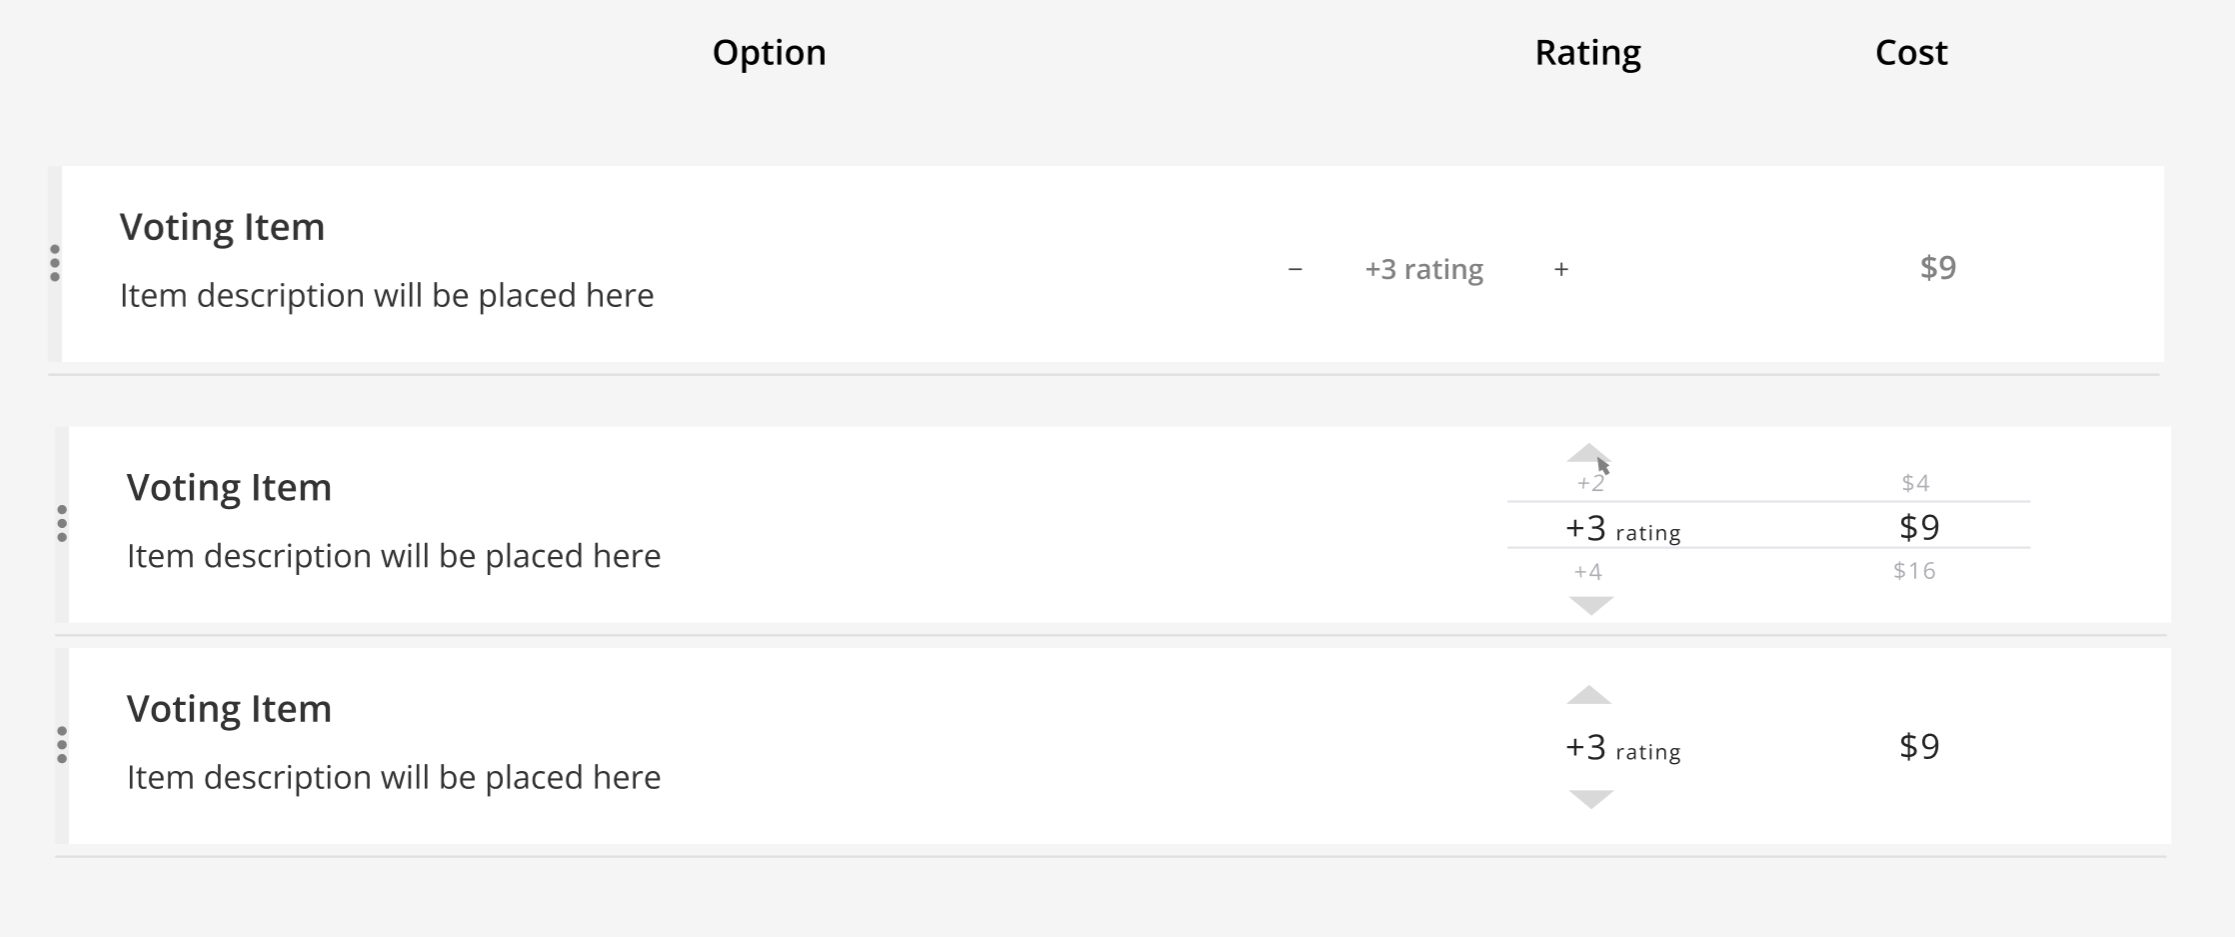
\includegraphics[width=0.8\textwidth]{content/image/prototypes/btn_design.png}
    \caption{Alternative vote control. The click-based design (upper) mirrors traditional vote control used in other QV interfaces, where each click controls one vote. The wheel-based design (the latter two) allows control through both clicks and mouse wheel rotation.}
    \Description{Three voting control interfaces are displayed. Each row represents a different interface. The first row shows a traditional click-based voting interface with options to decrease, increase, or maintain a rating of +3. The second and third rows show a wheel-based voting interface with mouse wheel functionality. In these, the middle row indicates a current rating of +3, with +2 and +4 ratings also visible. The cost for each option is listed on the right, ranging from 4 to 16. The last row mirrors the previous one with a rating of +3 and a cost of 9.}

    \label{fig:btn_design}
\end{figure}

\begin{figure}[ht]
    \centering
    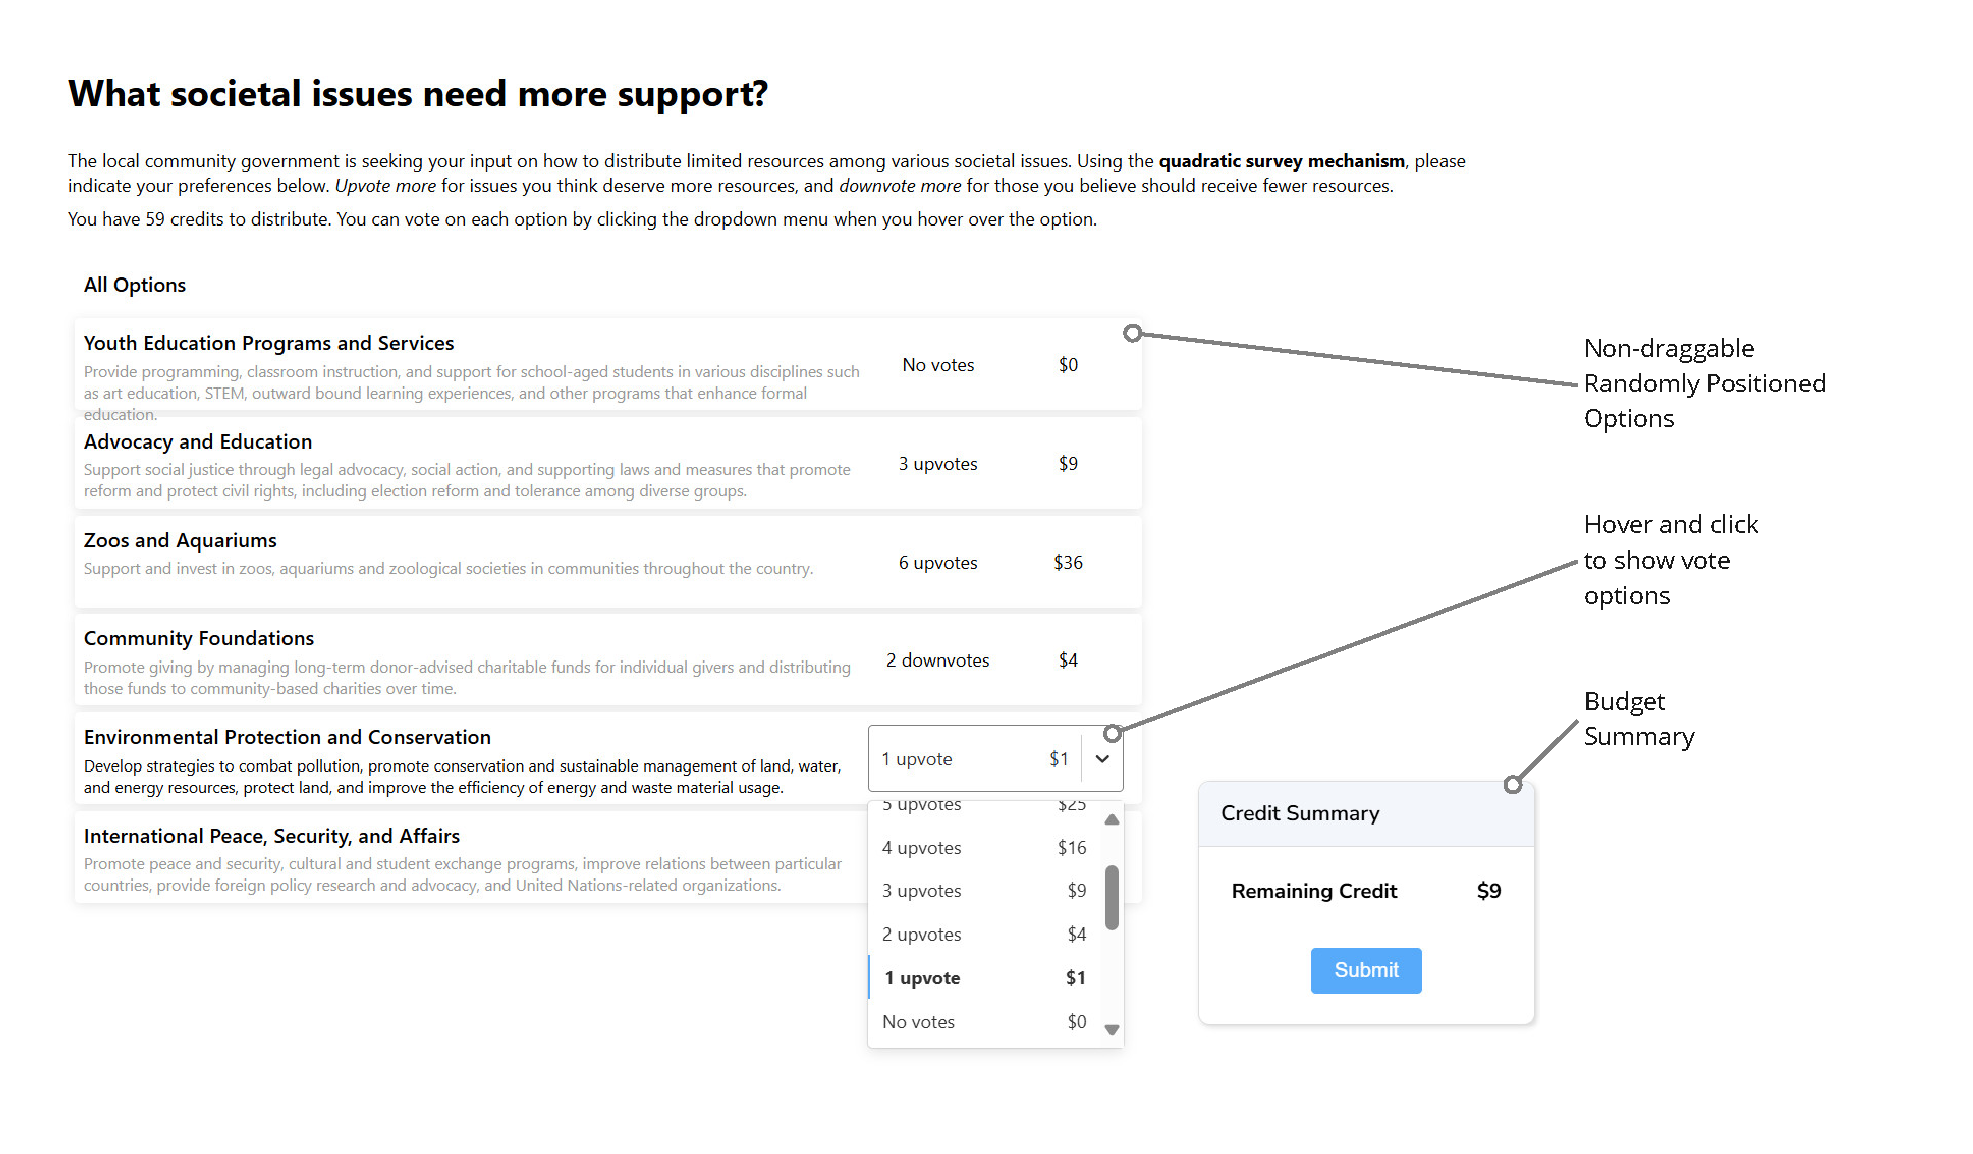
\includegraphics[width=\textwidth]{content/image/detailed_text.pdf}
    \caption{The text-based interface: This interface is based on the interactive version but does not include the two-phase interactive support and lacks the drag-and-drop functionality. Options are randomly positioned.}
    \Description{An image of a voting interface asking users to select societal issues needing support. The title reads, "What societal issues need more support?" with a brief explanatory paragraph underneath. Below, a list of six options is displayed, including "Youth Education Programs and Services," "Advocacy and Education," "Zoos and Aquariums," "Community Foundations," "Environmental Protection and Conservation," and "International Peace, Security, and Affairs." Each option has a description, a current vote count, and a dollar amount. The right side of the image shows an expanded dropdown menu for one of the options with selectable voting choices, such as "1 upvote" and "2 upvotes." A separate box labeled "Credit Summary" shows the remaining credit of 9 and a "Submit" button below it.}
    \label{fig:textInterface}
\end{figure}

\subsection{Baseline Interface: Single-Phase Text Interface} ~\change{We implemented the single-phase text interface (referred to as text interface for short) as our control condition to compare how the interactive components influenced participants' cognitive load and behavior. The text-based interface, like all existing interfaces, contains a list of static elements, a summary box, and a vote control. We followed the same design considerations, removing visual elements, presenting all options in the same screen, and using the dropdown for vote control, following the two-phase interface interface to provide a more direct comparison. We position the question prompt at the top followed by a randomly ordered option list to prevent ordering bias~\cite{ferberOrderBiasMail1952, couperWebSurveyDesign2001} below. Individual option costs and the remaining credits' summary box are presented to the right of the screen given our interface layout.}

Both experimental interfaces were developed with a ReactJS frontend and a NextJS backend powered by MongoDB. We open-source both interfaces.\footnote{link-to-github}


% In our first prototyped tool, we aim to help survey respondents rank options to establish relative preferences before voting. As shown in Figure~\ref{fig:qv_rank}, our prototype allows respondents to move options before finalizing their votes. During our pretest, we found that respondents rarely moved the options and some questioned the need for a full ranking since it did not affect the QS submission. Many did not realize the options were draggable until we pointed it out. The main insight from this prototype is that creating a full rank is~\textit{not} essential for establishing~\textit{relative} preferences, leading us to consider selecting a subset of options instead of requiring a full rank among all options.

% First, we surveyed the current implementation of QV interfaces to understand the development of such tools. We presented a selection in Figure~\ref{fig:qv_interface_external}. All five interfaces retained and presented the following components:
% \begin{itemize}
%     \item Option list: A list of options contesting for votes.
%     \item Vote Controls: Two buttons to increase and decrease votes associated with each option.
%     \item Individual vote tally: A representation of votes associated with an option.
%     \item Summary: A summary that automatically calculated the cost across options and the remaining budget.
% \end{itemize}
% Now we present the final interactive interface and describe how it operates. In this subsection, we provide supporting evidence from prior literature that we previously omitted. These pieces of literature were omitted for clarity and focus in the previous subsection but will be reintroduced here. 
% We constructed a text-based interface that included all five components but removed the use of emojis (i.e., thumbs up and thumbs down present in Figure~\ref{fig:wedesignInterface}), progress bars, and other visualizations in the summary section (i.e., progress bars in Figure~\ref{fig:wedesignInterface} and~\ref{fig:chengInterface} or blocks presented in Figure~\ref{fig:rxcvotingInterface}), and the visual cues for individual vote counts (i.e., the colored counts and icons present in Figure~\ref{fig:gov4gitInterface} and~\ref{fig:chengInterface}).

% During this process, we noticed several issues. First, many survey respondents placed most options into the 'option you care about' category, defeating the design's purpose. Second, there were no indicators distinguishing between the selected and remaining options. Respondents did not notice their selections were kept at the top in the voting stage and were unsure why Step 1 was necessary if all options were shown again. This informed two takeaways: selecting options to vote on is too coarse to construct relative preferences, and there needs to be a clearer distinction and connection between the two phases.

% Feedback indicated that survey respondents are comfortable with this two-phase organize-then-vote design. Several user experience issues emerged, but they were addressable without significantly modifying this interaction structure. These issues include: First, dragging and dropping all options into different categories is cumbersome and can mislead respondents into thinking this is a ranking process, which is not the goal. Second, the position of unorganized options at the top of the voting list is counterintuitive. Third, the voting controls are disconnected from the option summaries, dividing attention between the left and right sides of the screen.

% These design decisions led to the interface shown in Figure~\ref{fig:textInterface}. 


% \subsubsection{Paper prototype: visualizing trade-offs}
% The original paper prototype aimed to help visualize survey respondents' tradeoffs among options. 
% The original paper prototype aimed to utilize visual representations to highlight the constrained availability of credit and to explain the costs and trade-offs associated with selecting each available option.
% Early on, we did not know which components made QS more difficult than other survey techniques. We began by surveying existing interfaces (Figure~\ref{fig:qv_interface_external} other than Figure~\ref{fig:gov4gitInterface} which did not exist near the writing of this paper). All four interfaces consist of these common components:
% As we were unsure what made QS more complex than other survey techniques, our investigation began with the existing interface (Figure~\ref{fig:qv_interface_external}, except Figure~\ref{fig:gov4gitInterface} which did not exist at that time. All four interfaces consist of these common components:
% \begin{itemize}
%     \item Option list: A list of options contesting for votes.
%     \item Vote Controls: Buttons to increase and decrease votes associated with each option.
%     \item Individual vote tally: A representation of votes associated with an option.
%     % \item Summary: A summary that automatically calculates the cost across options and the remaining budget.
%     \item Summary: An auto-generated summary of costs and remaining budget.
% \end{itemize}

% To brainstorm ways to help survey respondents manage trade-offs across options, we decomposed these options and explored several innovative layouts. Initially, we thought trade-offs were the core cause of cognitive load. In this paper, we show two versions of the paper prototypes in Figure~\ref{fig:qv_paper}. In both figures, costs are represented by blocks, similar to Figure~\ref{fig:rxcvotingInterface}. We imagine the survey respondents to drag and position options in the space provided unstructurally (Figure~\ref{fig:horizontal_paper}) or structurally (Fig~\ref{fig:vertical_paper}). Similar to the seminal debate on direct manipulation vs. interface agents~\cite{shneidermanDirectManipulationVs1997}, the research team was unsure how much control survey respondents should have over the positioning of the options to aid the decision-making process that considers trade-offs. Different from prior interfaces, we used placements of the interface to denote positive or negative number of votes. After several pretests, we learned that the main process participants aim to do throughout the survey is establishing~\textit{relative} preferences across the options, rather than thinking so much about trade-offs. 
% To further explore the features that contribute most to the complexity of QS, we developed two prototypes shown in Figure~\ref{fig:qv_paper}. Similar to Figure~\ref{fig:rxcvotingInterface}, these prototypes use blocks to represent costs, arranged either unstructurally (Figure~\ref{fig:horizontal_paper}) or structurally (Fig~\ref{fig:vertical_paper}), facilitating the visualization of the trade-offs. Unlike previous interfaces, we utilized the placement of the interface to denote positive or negative vote counts. Several protests indicated that participants primarily focus on establishing relative preferences among options rather than trade-offs. Therefore, in this study, we focused on enhancing designs that facilitate the establishment of relative preferences.
% the two main features of QS we identified are the relative preference through a combined presentation of rankings and ratings, and the option selection trade-offs due to total credit limits. 
% The initial prototyping involves collecting the interface designs for existing quadratic mechanism-based software. Iterative pretests informed each subsequent design. We present these iterations, which aim to enhance user experience in the preference construction process in the following sections.

% In the previous subsection, we highlighted critical prototype iterations that informed the final two-phase interactive process that defines the user journey. 
% We now present the final two-phase interface, its operations, and the supporting literature for comprehensive understanding.
% Then, We also discuss the aesthetic design choices that emerged throughout the iterations.

\begin{figure}[ht!]
    \centering
    % Top figure (full-width)
    \begin{subfigure}{\textwidth} % Full width for the first subfigure
        \centering
        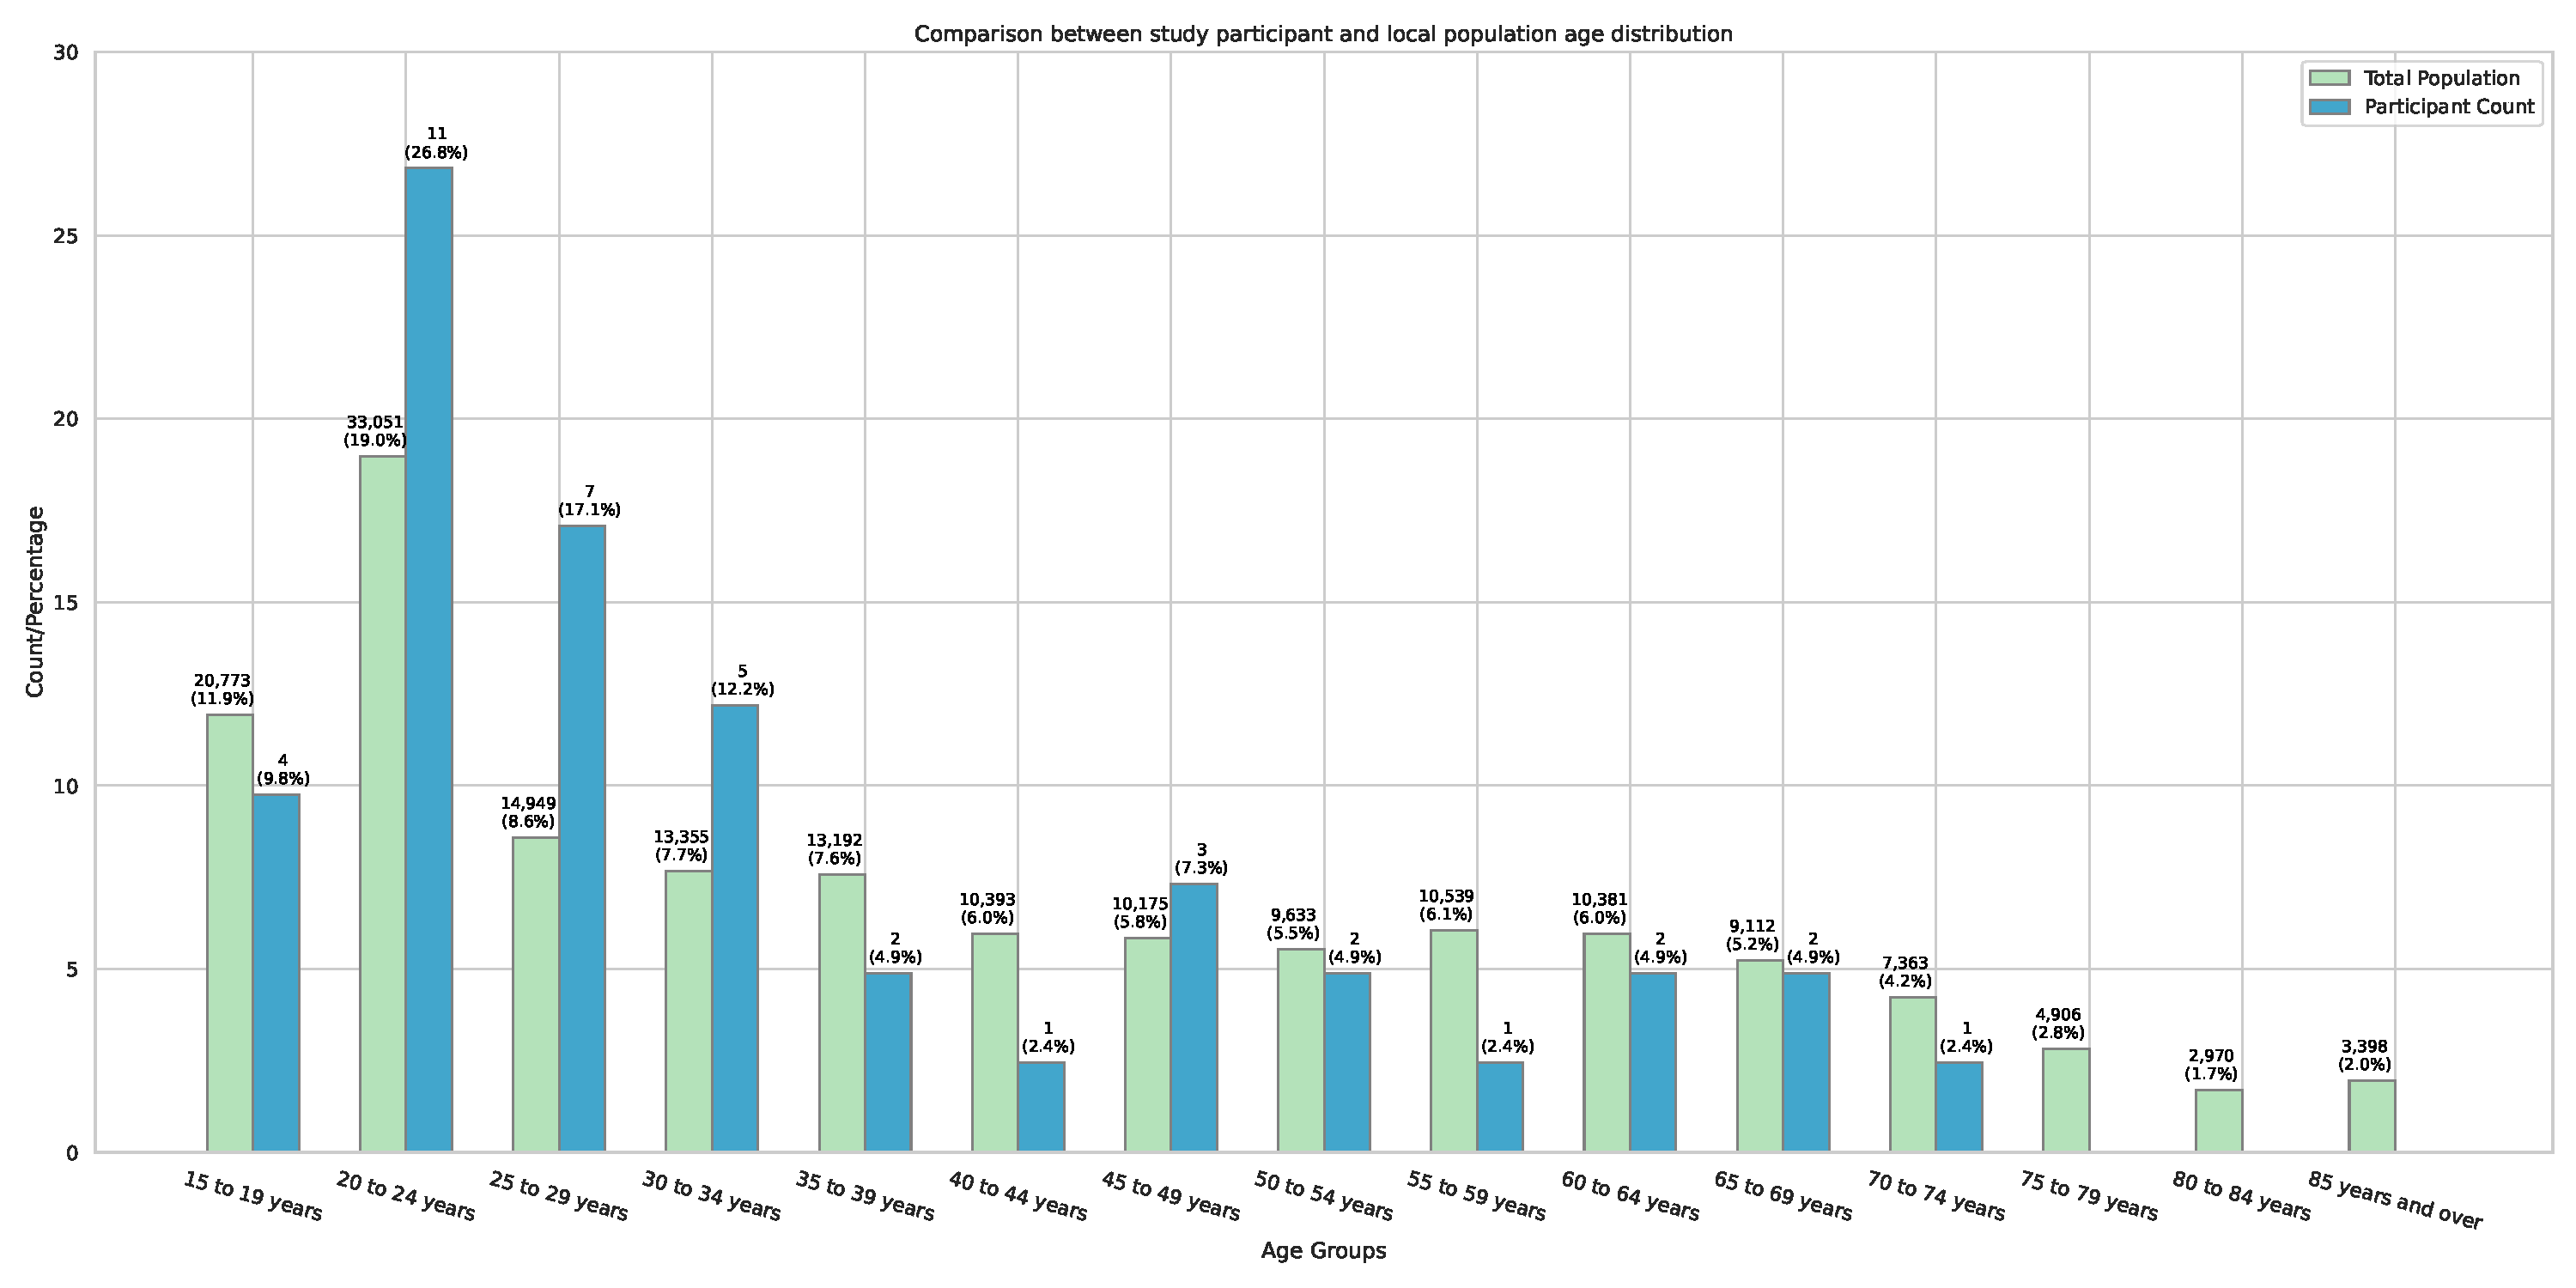
\includegraphics[width=\textwidth, trim=0 13 0 13, clip]{content/image/demo/demo_age_group_vertical.pdf}
        \caption{Age distribution of the study participants were similar to the locale's demographic profile.}
        \Description{A bar chart comparing the age distribution between study participants and the local population. The x-axis represents age groups from 15-19 to 85+, and the y-axis shows count/percentage values ranging from 0 to 30. Each age group has two bars: one for the total population (in peach) and one for participant count (in light blue). Some key differences are visible, such as the 20-24 age group, where the total population is 33,051 (19\%) and participants are 11 (27\%). The 25-29 group shows 14,949 (9\%) for the population and 7 (17\%) for participants. Percentage and count data are displayed above each bar. Other age groups had similar bars. The chart title reads "Comparison between study participant and local population age distribution," and the legend distinguishes the two categories (Total Population and Participant Count).}
        \label{fig:demoAge}
    \end{subfigure}
    
    \vspace{0.25cm} % Add some vertical space between the subfigures

    % Bottom figures (two subfigures side by side)
    \begin{subfigure}{0.45\textwidth} % First subfigure on the second row
        \centering
        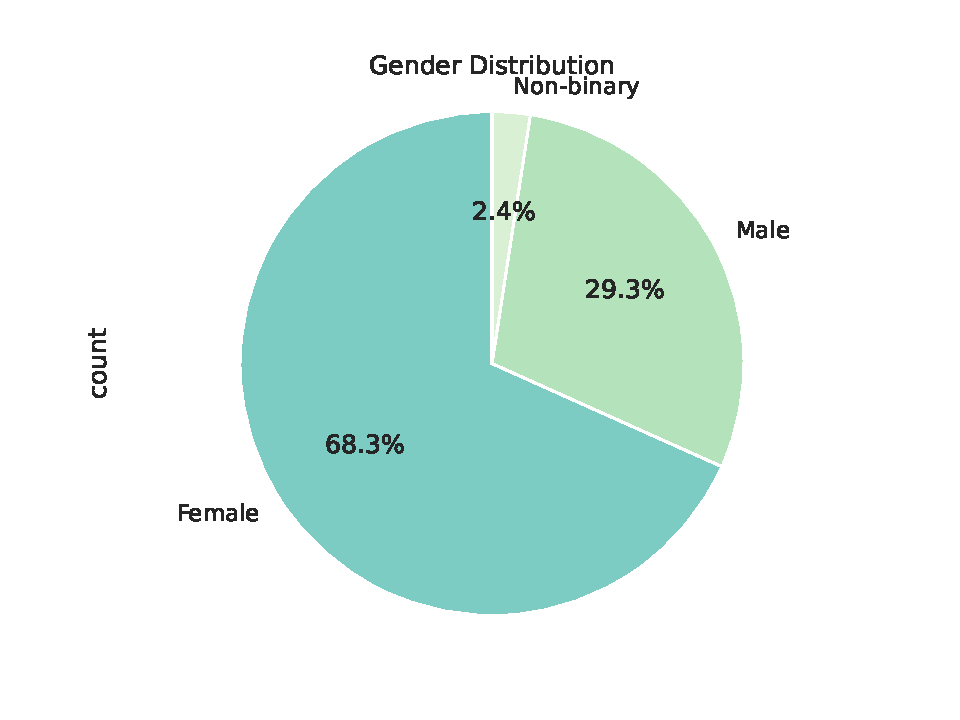
\includegraphics[width=\textwidth]{content/image/demo/demo_gender.pdf}
        \caption{Gender distribution of our participants skewed towards female participants.}
        \Description{A pie chart displaying the gender distribution of study participants. The chart is divided into three sections: 68.3\% (28 participants) are labeled as female and shown in blue, 29.3\% (12 participants) are labeled as male and shown in peach, and 2.4\% (1 participant) are labeled as non-binary, represented by a small gray slice. The title reads "Participant Gender Distribution," and the y-axis on the left is labeled "\% of Participant (Count)."}
        \label{fig:demoGender}
    \end{subfigure}
    \hfill
    \begin{subfigure}{0.45\textwidth} % Second subfigure on the second row
        \centering
        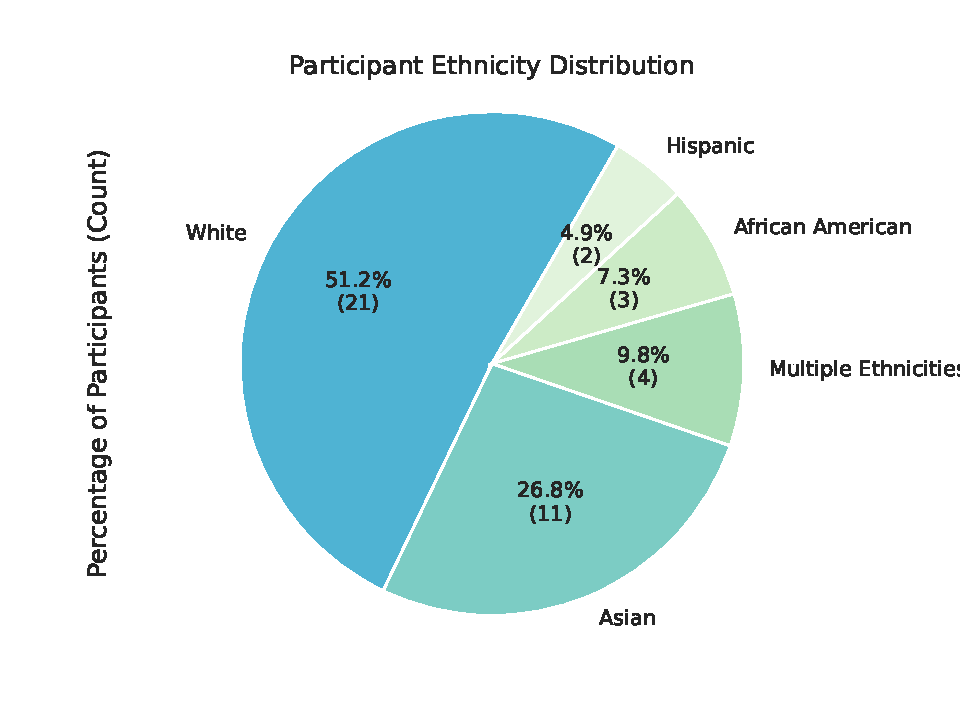
\includegraphics[width=\textwidth]{content/image/demo/demo_ethnicity.pdf}
        \caption{Ethnicity distribution remains diverse with fewer Hispanic and African American participants.}
        \Description{A pie chart showing the ethnicity distribution of participants. The largest segment, representing 51.2\% (21 participants), is labeled White and shown in light blue. Other segments include 26.8\% (11 participants) for Asian, 9.8\% (4 participants) for Multiple Ethnicities, 7.3\% (3 participants) for African American, and 4.9\% (2 participants) for Hispanic. The percentages and counts are displayed within each section. The y-axis on the left is labeled "\% of Participants (Count)," and the title reads "Participant Ethnicity Distribution."}
        \label{fig:demoEthnicity}
    \end{subfigure}

    \caption{Demographic distributions: Age, Gender, and Ethnicity}
    \Description{A collection of three demographic graphs demonstrating age, gender and ethnicity distribution.}
    \label{fig:Demographics}
\end{figure}


\begin{figure}[ht!]
    \centering
    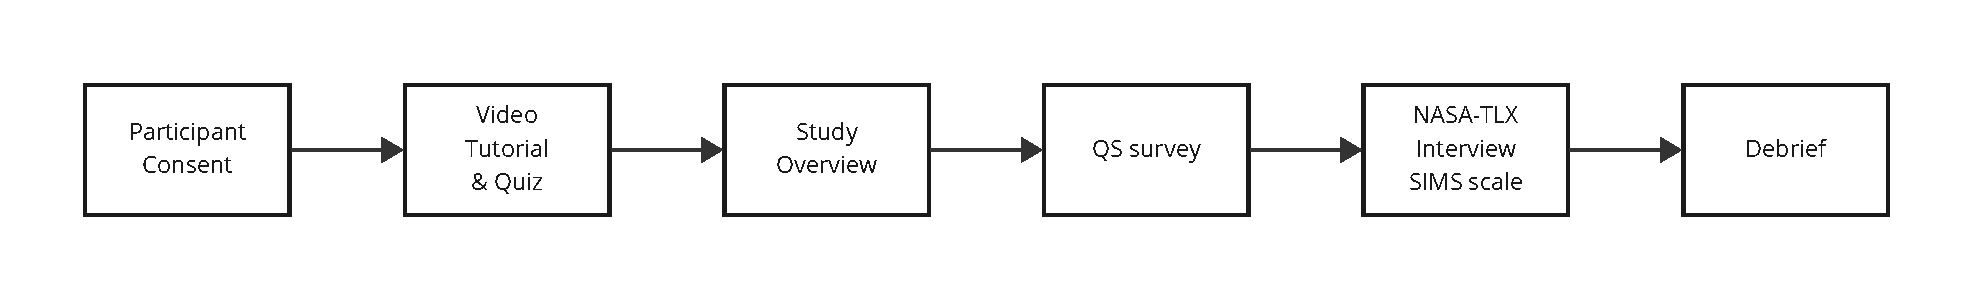
\includegraphics[width=1\textwidth]{content/image/study_flow.pdf}
    \caption{Study protocol: Participants are asked to learn about the mechanism of QS after consenting to the study. The researcher explained the study overview and asked participants to complete the QS. A NASA-TLX survey followed by interviews to understand participants' cognitive load. We debriefed participants after the study.}
    \Description{A flowchart depicting the study protocol, consisting of six stages. Each stage is represented by a rectangular box connected by right-facing arrows. The boxes, from left to right, are labeled: "Participant Consent," "Video Tutorial \& Quiz," "Study Overview," "QS," "NASA-TLX Interview," and "Debrief." The arrows between the boxes indicate the sequence of the study process.}

    \label{fig:studyProtocol}
\end{figure}

\section{Experiment Design}
\label{sec:experiment}
We recruited $41$ participants, with one excluded\footnote{The participant reported not completing the survey seriously because they believed the experiment was fake.} due to data quality concerns, from a United States college town using online ads, digital bulletins, social media posts, online newsletters, and physical flyers in public spaces beyond campus. To ensure participant diversity, we prioritized non-students by selectively accepting them as we monitored demographics. Study participants' mean age was~$34.63$ years old, with an age distribution similar to the county's demographic profile~(Figure~\ref{fig:demoAge}) albeit a slightly higher representation of younger adults.~\change{Demographic between groups (see Appendix \ref{sec:apdx:demo}) are reasonbally balanced, with short text interface participants skew slightly younger.} Gender and race demographics are aggregated in Figure~\ref{fig:demoGender} and~\ref{fig:demoEthnicity}. The study was framed as focusing on societal attitudes to avoid response bias. The university's Institutional Review Board reviewed and approved this study. 
% In the following section we detail the experiment design and rationale.
% If a respondent self-identified as a student, we thanked them and informed them of our current priority for non-students, though some self-identified students were still accepted.
% \subsection{Experiment Protocol}

Figure~\ref{fig:studyProtocol} visually represents the study protocol. Participants completed the study in the lab to control for external influences. Participants used a 32-inch vertical monitor displaying all options. After consenting, participants watched a video explaining the quadratic mechanism without hints of interface operation followed by a quiz to ensure understanding. Participants rewatched the video or consulted the researcher until they could select the correct answers. The participant's screen was captured throughout the study. The researcher primed the participant that the study aimed to help local community organizers understand preferences on societal issues to better allocate resources. Participants were randomly assigned to one of four groups:

\begin{itemize}
    \item Short Text (ST): A text interface with $6$ options. ($N=10$)
    \item Short Two-Phase (SP): A two-phase interface $6$ options. ($N=10$)
    \item Long Text (LT): A text-based interface $24$ options. ($N=10$)
    \item Long Two-Phase (LP): A two-phase interface with $24$ options. ($N=10$)
\end{itemize}

Participants completed the survey independently, without the researcher's presence. They then contacted the researcher for the NASA-TLX survey, followed by a short audio-recorded semi-structured interview. The session concluded with a debriefing and a \$15 cash compensation, during which participants were informed of the study goal on cognitive load and interface design.

We made several experimental design choices. First, we selected a between-subject design to minimize study fatigue, considering the complexity of QS, and avoiding the learning effect that could influence how participants evaluated the options. Second, we chose the context of public resource allotment, where participants expressed their preferences regarding their preference across $6$ or $24$ societal issue options, following the methodology of ~\textcite{chengCanShowWhat2021}. These issues are relevant to all citizens and effectively demonstrate the need to prioritize limited public resources. We curated $26$ societal issues used by Charity Navigator~\cite{CharityNavigator2023} which evaluates over $20,000$ charities in the United States. The interface randomly presents options from this list to participants,~\change{ensuring that no systematic content differences affected participant responses. This randomization serves to control for any potential biases that different voting options might introduce between the short and long versions}. Appendix~\ref{sec:charityList} contains the full list.

We decided to test $6$ and $24$ options, representing short and long lists, as identifying the `breaking point' for cognitive overload would require impractical time and resource commitments. Constant sum surveys and the Analytic Hierarchy Process (AHP) recommend fewer than ten and seven options, respectively~\cite{moroneyQuestionnaireDesignHow2019, saatyGroupDecisionMaking2013, saatyPrinciplesAnalyticHierarchy1987}.~\textcite{millerMagicalNumberSeven1956}'s classic work on cognitive processing capacity and~\textcite{saaty2003magic}'s theoretical proof supported the use of $7\pm2$ items. A meta-analysis by~\textcite{chernevChoiceOverloadConceptual2015} identified $6$ and $24$ as common values for short and long lists in choice overload studies, rooted in the original experiment by~\textcite{iyengarWhenChoiceDemotivating2000}.

Finally, we deployed self-report subjective surveys and analytical measures (i.e., time and clickstream data). We adopted the paper-based weighted NASA Task Load Index (NASA TLX), a widely used multidimensional tool that averages six subscale scores to represent overall workload after completing a task~\cite{hart1988development, hartNasaTaskLoadIndex2006, cain2007review}. NASA-TLX is favored for its low cost and ease of administration~\cite{gaoMentalWorkloadMeasurement2013}, with less variability compared to one-dimensional workload scores~\cite{rubioEvaluationSubjectiveMental2004}, making it suitable for our study. \change{While cognitive load can be assessed through performance, psychophysiological, subjective, and analytical measures~\cite{gaoMentalWorkloadMeasurement2013}, the length and complexity of QS make some of these impractical. Performance and analytical measures requires task switching or interruption risking additional overall cognitive load and additional experiment time. Psychophysiological measures like pupil size~\cite{palinkoEstimatingCognitiveLoad2010} and ECG~\cite{haapalainenPsychophysiologicalMeasuresAssessing2010} are costly, sensitive to external factors, and often requires participants to wear additional devices.}

% performance measures using a secondary task were impractical. Psychophysiological measures such as pupil size~\cite{palinkoEstimatingCognitiveLoad2010} and ECG~\cite{haapalainenPsychophysiologicalMeasuresAssessing2010} were costly and sensitive to external factors. 


 % The complexity of QS survey made completing back-to-back studies impractical. Since preferences are constructed, we wanted to ensure that participants were not influenced by their previous preferences, which could affect their perceived cognitive load and decision-making process.

% asking participants to revisit the lab after several days would likely increase dropout rates and demotivate participants from attending in-person sessions. Second, we aimed to reduce the learning effect, which is challenging to eliminate, especially concerning interface operation and decision-making in the survey. 

% Thus, we adopted these values to align with prior research. \footnote{We believe that the original value decision was due to the limitations of the jam flavors.}

% 

% Therefore, we deployed self-report subjective surveys and analytical measures (i.e., like time and clickstream data). We adopted the paper-based weighted NASA Task Load Index (NASA TLX), a widely used multidimensional tool that averages six subscale scores to represent overall workload after completing a task~\cite{hart1988development, hartNasaTaskLoadIndex2006, cain2007review}. Despite some criticisms, NASA-TLX is favored for its low cost, ease of administration~\cite{gaoMentalWorkloadMeasurement2013}, and significantly less variability compared to one-dimensional workload scores~\cite{rubioEvaluationSubjectiveMental2004}, making it suitable for our study.


% Finally, participants complete the situational motivation scale (SIMS) to gauge motivation and a demographic survey.
% Last, we describe the two quantitative measurements taken during the study: cognitive load and motivation. 
% , indicating differences in workload definitions among raters within a task and variations in workload sources between tasks

% Tabling SIMS for now. It was not used in the analysis. In addition to NASA-TLX, we administered a situational motivation scale (SIMS) to measure participants' motivation (required citation). We posited that motivation would influence mental demand (required citation). SIMS, chosen for its widespread use, helps understand one's intrinsic motivation, extrinsic motivation, identified regulation, and external regulation, and was originally designed to measure self-determination. Both instruments were administered using pen-and-paper.

% The reason we made this experiment design decision was to minimize . External factors, more prevalent in remote experiments or those conducted via platforms like MTurk, included potential multitasking or interruptions by others. An in-lab study also allowed participants to operate across a consistent device that researchers had full control over.
\section{Results}
\label{sec:result}
In this section, we present the results of our study, which are organized as follows: We begin with a description of participant demographics, followed by quantitative and qualitative assessments of cognitive load. We then provide a detailed analysis of participant behaviors. The section concludes with qualitative insights derived from participants' comments on their experiences and the interfaces used. Quantitative data were derived from pen-and-paper surveys and system logs captured during the study. Qualitative insights were generated from interviews conducted after participants completed the survey task. Interview were transcribed and thematically analyzed by the first author. All processed behavioral data are publicly available\footnote{link-to-github} to support transparency and facilitate further research.

\begin{figure}[ht]
    \centering
    % Top figure
    \begin{subfigure}[b]{\textwidth}
        \centering
        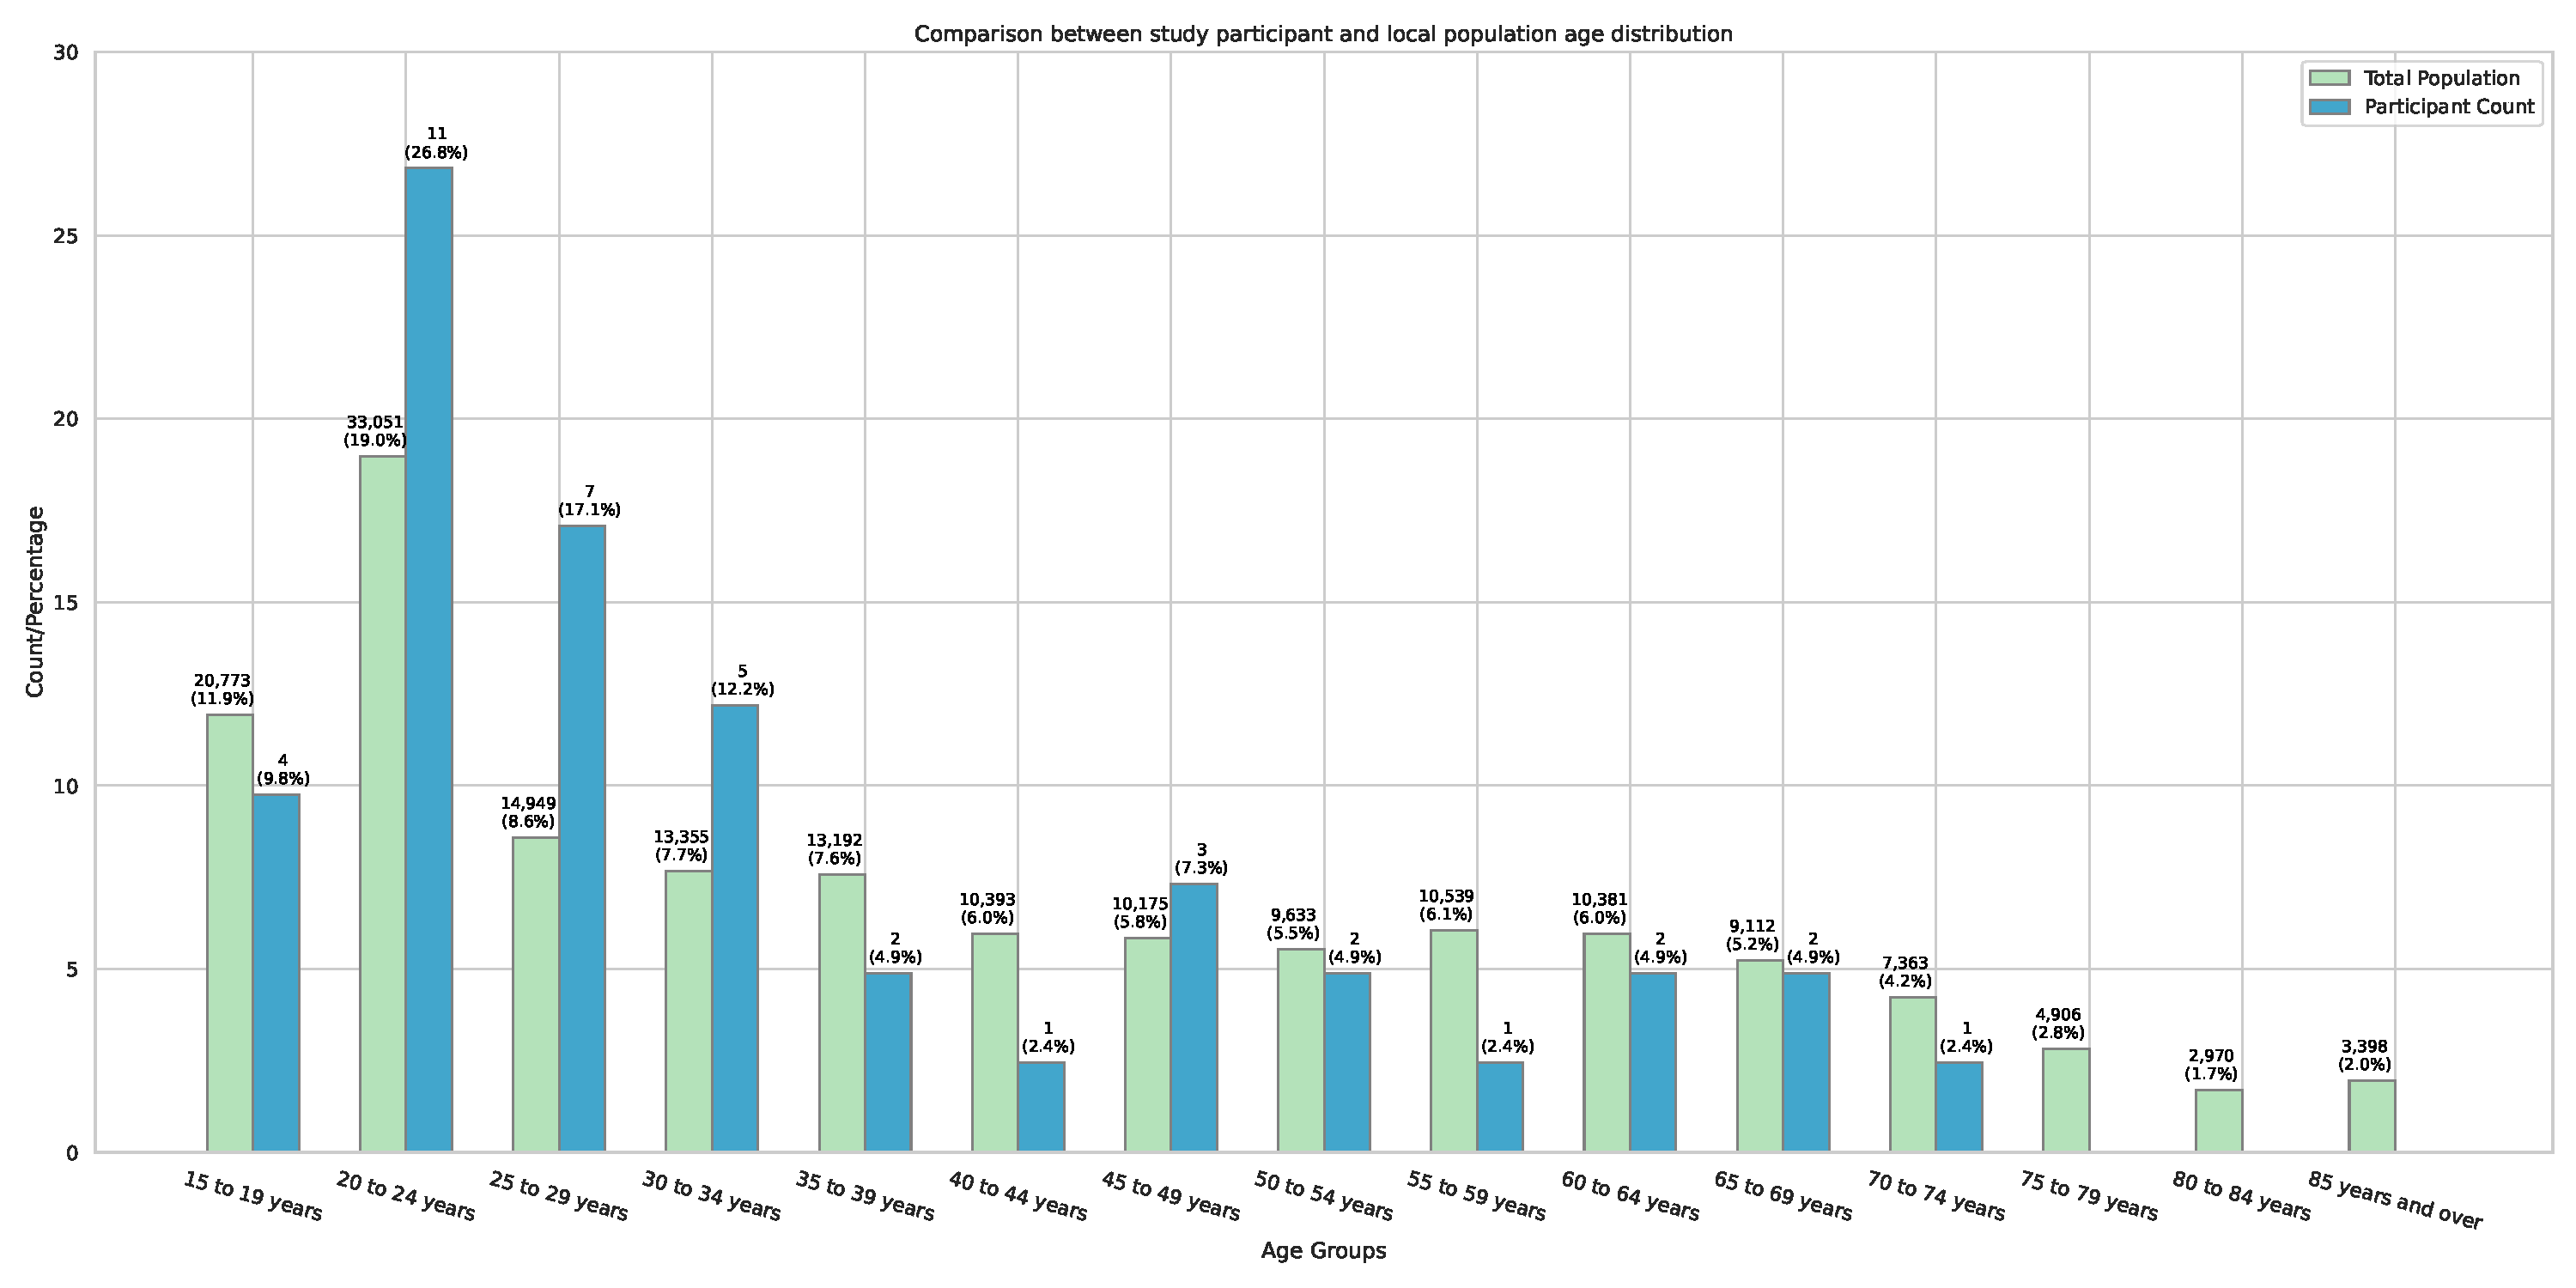
\includegraphics[width=\textwidth]{content/image/demo/demo_age_group_vertical.pdf}
        \caption{Age distribution}
        \label{fig:demoAge}
    \end{subfigure}
    
    \vspace{0.5cm} % Add some vertical space between the rows

    % Bottom figures
    \begin{subfigure}[b]{0.45\textwidth}
        \centering
        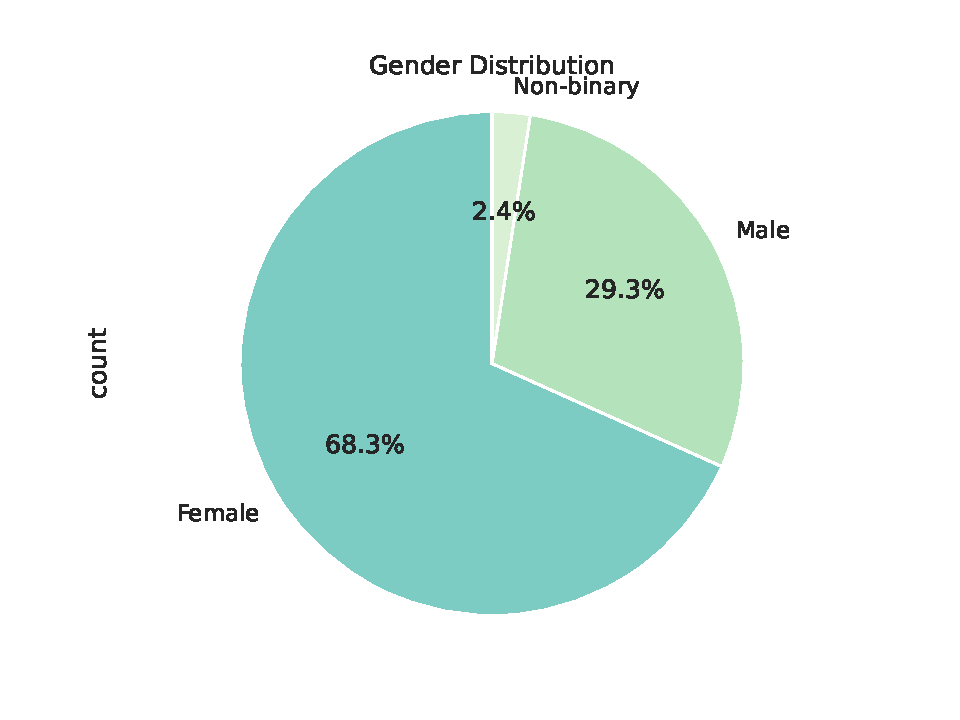
\includegraphics[width=\textwidth]{content/image/demo/demo_gender.pdf}
        \caption{Gender distribution}
        \label{fig:demoGender}
    \end{subfigure}
    \hfill
    \begin{subfigure}[b]{0.45\textwidth}
        \centering
        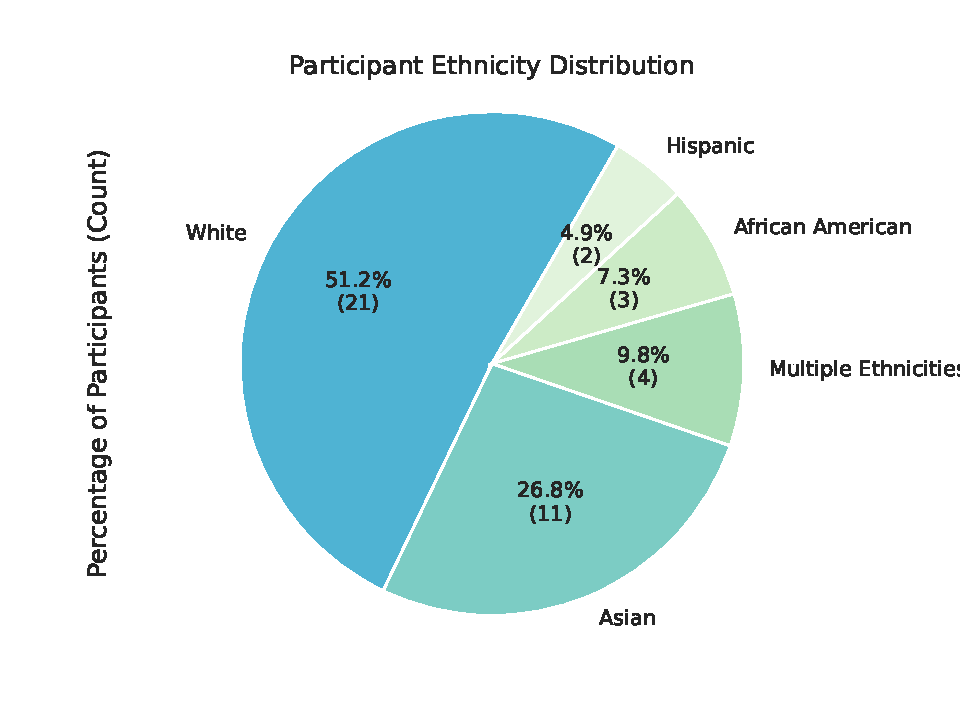
\includegraphics[width=\textwidth]{content/image/demo/demo_ethnicity.pdf}
        \caption{Ethnicity distribution}
        \label{fig:demoEthnicity}
    \end{subfigure}
    
    \caption{Demographic distributions: Age, Gender, and Ethnicity}
    \label{fig:Demographics}
\end{figure}

% maybe more the figure to the appendix?

\subsection{Demographics}
We recruited a total of $41$ participants, allocating ten to each experiment condition. Due to data quality concerns, we excluded one participant's data. The mean age of the participants was $34.63$ years old, with a detailed age distribution presented alongside the county population distribution in Figure~\ref{fig:demoAge}. This comparison reveals that our sample closely matches the county's demographic profile, albeit with a slightly higher representation of younger adults, particularly in the 35-45 age range. As shown in Figure~\ref{fig:demoGender}, the majority of participants skewed toward female.

Regarding ethnicity, $51.2\%$ of the participants identified as White, $26.8\%$ as Asian, $7.3\%$ as African American and $4.9\%$ as Hispanic. Additionally, $9.8\%$ of participants reported mixed ethnicity.

\subsection{Cognitive Load Results}
\label{sec:cog}
In this subsection, we present results in the order of the research questions. We first discuss the distribution of the aggregate NASA-TLX scores across the four experiment conditions, providing interpretation of the results to answer RQ1 and RQ2a. Next, we report the NASA-TLX scores disaggregated into their composite six dimensions to answer RQ2b. Then, we present qualitative and quantitative findings on user behavior for RQ3. Finally, we present additional comments from participants regarding the interfaces.

\begin{figure}[ht]
    \centering
    \begin{subfigure}[b]{0.45\textwidth}
        \centering
        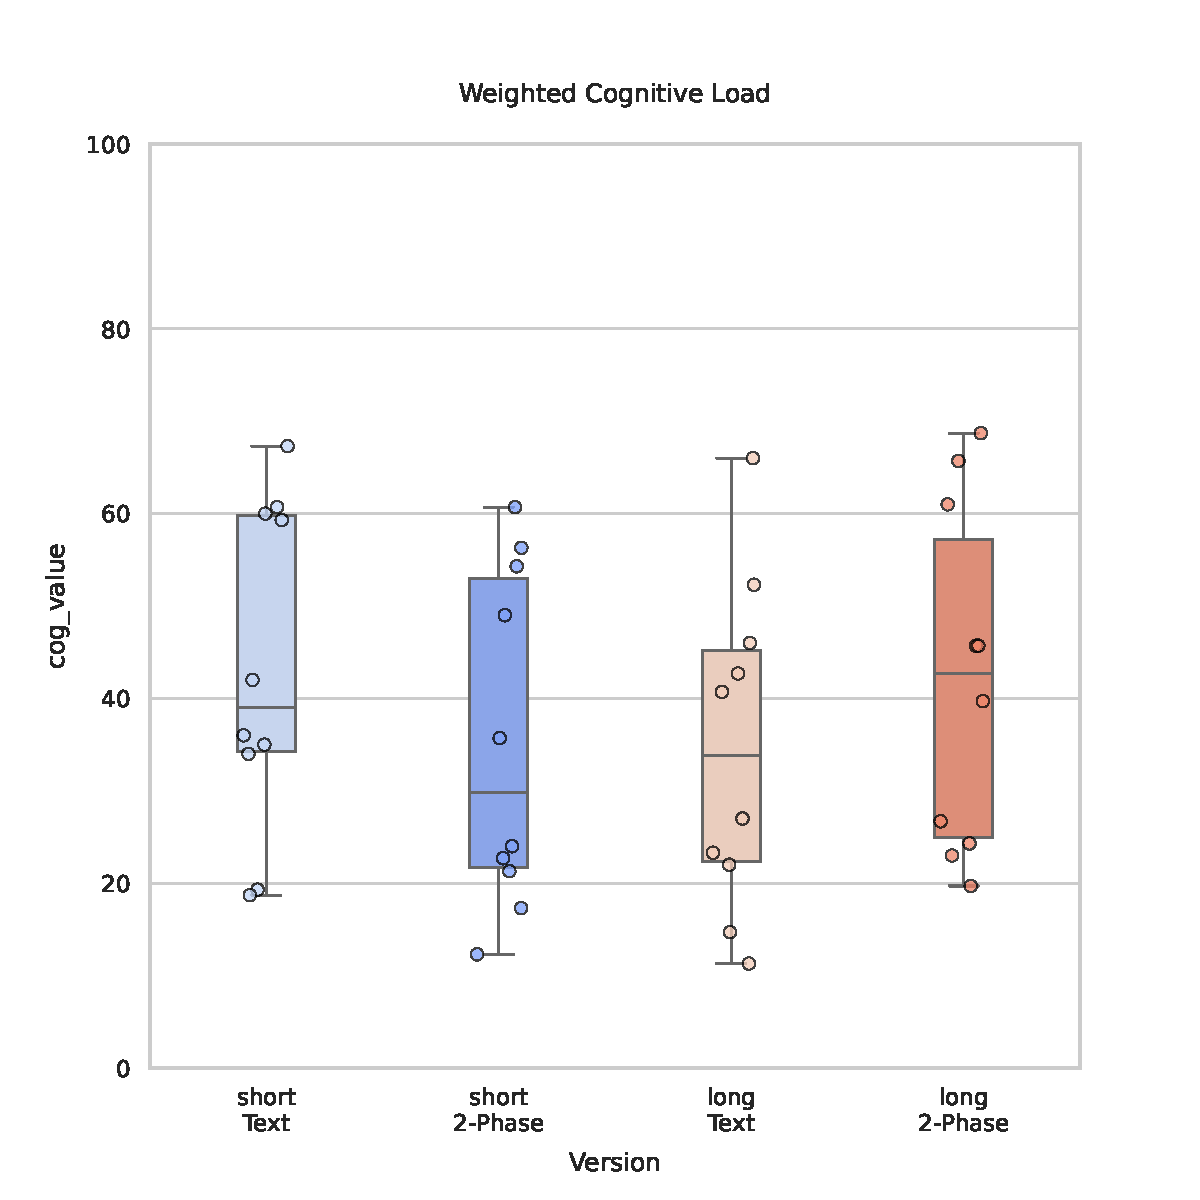
\includegraphics[width=\textwidth]{content/image/results/nasatlx_final_value.pdf}
        \caption{NASA-TLX Weight Score Distribution}
        \label{fig:nasatlx-final1}
    \end{subfigure}
    \hfill
    \begin{subfigure}[b]{0.47\textwidth}
        \centering
        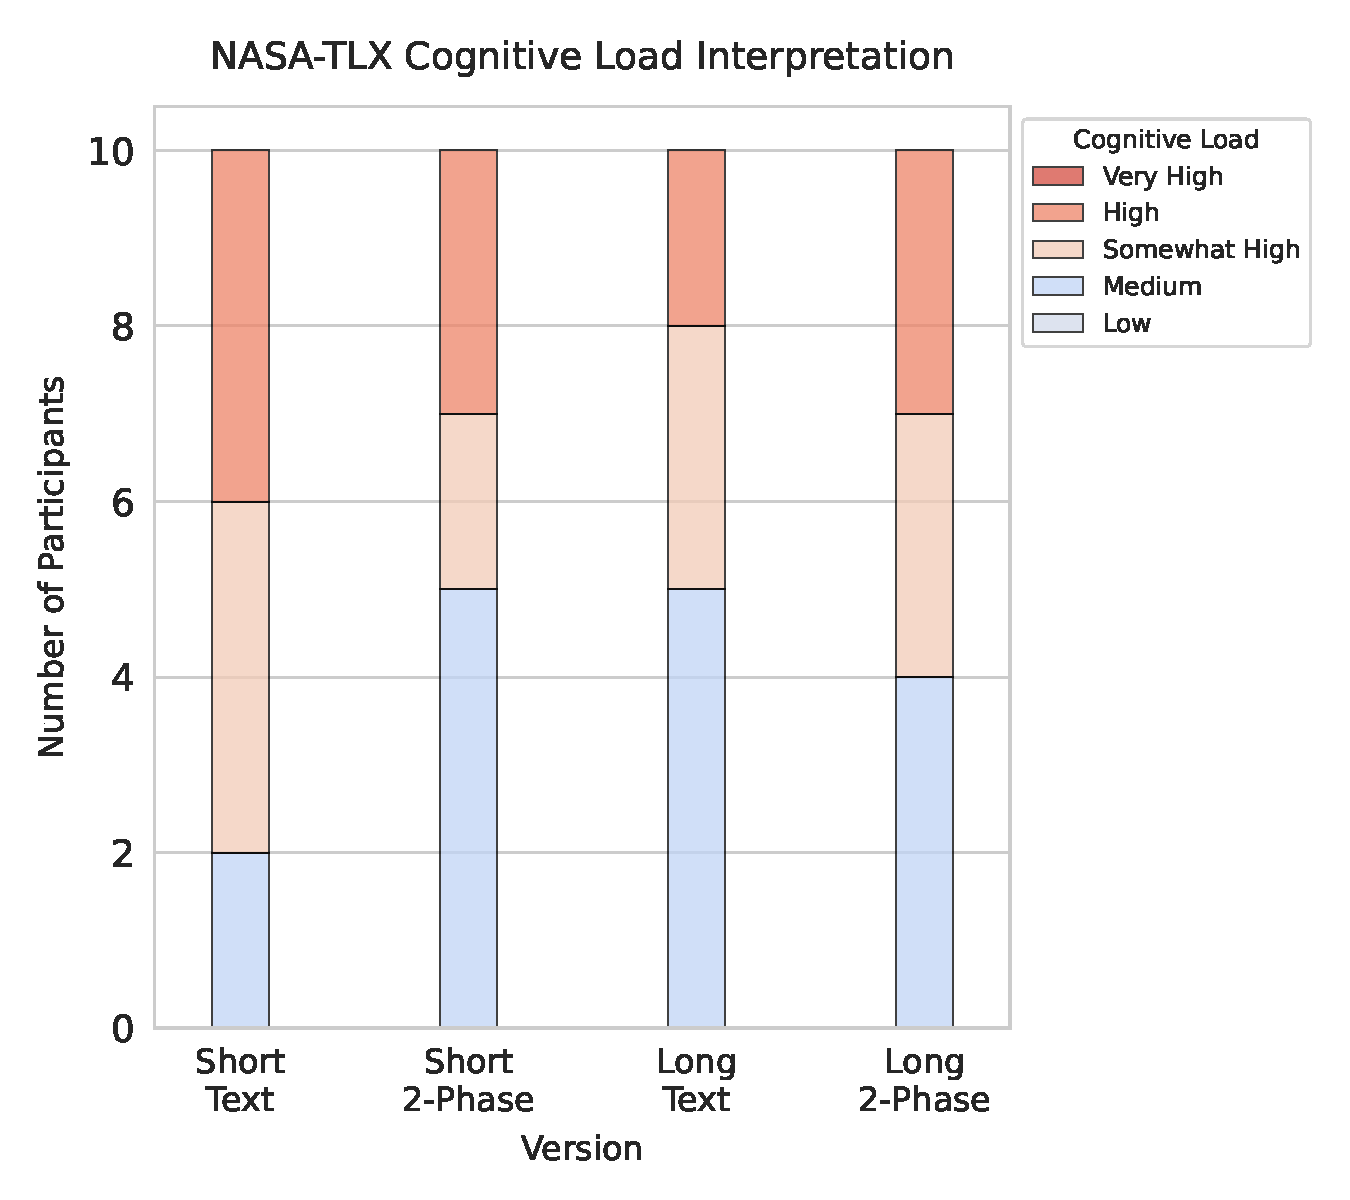
\includegraphics[width=\textwidth]{content/image/results/nasatlx_cog_value_interpreted.pdf}
        \caption{NASA-TLX Cognitive Interpretation}
        \label{fig:nasatlx-final2}
    \end{subfigure}
    \caption{NASA-TLX Results}
    \label{fig:nasatlx-final}
\end{figure}

We show the NASA-TLX weighted results in Figure~\ref{fig:nasatlx-final1}. A higher value refers to higher cognitive load. Qualitatively, the interactive interfaced decreased the cognitive load for the short survey, but seems to have increased the cognitive load for the long survey. A Mann-Whitney U-Test indicates that these differences are not statistically significant. We follow predefined mappings of NASA-TLX values to cognitive levels: low, medium, somewhat high, high, and very high, as listed by ~\textcite{hart1988development}. We show value interpretations in Figure~\ref{fig:nasatlx-final2}. The short text interface had the most participants ($N=8$) rating their cognitive experience as somewhat high or above. The other three experiment groups showed similar cognitive load with about half of the participants experiencing medium cognitive load and the others experiencing somewhat high or high loads. No participants in any conditions expressed experiencing very high cognitive loads.

These results partially answer our first two research questions. To our surprise, the longer survey did not introduce extraneous cognitive load despite the budget of the long QS increasing by 8 times and the options increasing fourfold. We deduct through a list of possible explainations. First, the interactive interface increases participants' cognitive load. However, we do not think this is the case. If it were, we would expect to see even more significant cognitive overload in the long interactive interface, resulting in lower cognitive load scores. Second, participants in the long text interface are cognitively overloaded, leading to satisficing behaviors due to the numerous decisions required to complete the task. We investigate if this is true in the following subsection. Third, we cannot rule out that the interface, contrary to our expectations, did not reduce cognitive load but rather shifts participants' cognitive load throughout the process of completing QS.

% TODO: MERGE INTO ABOVE PARAGRAPH :: Based on these results, given the small sample size for each group of participants, we were not surprised that most results do not provide statistical significance in changes in cognitive load values. However, there are some trends that we capture via descriptive statistics. First, comparing the overall cognitive load and the breakdown of the sub-components between text interface and interactive interface across the short survey, we see a general trend in a reduction of cognitive load. Next, we are surprised by the upward trend between the text and interactive interface for the longer list. This is against our original hypothesis that under even complex situations, we should see a clearer portrait of how interactive interactions can reduce cognitive load. While it is possible that interactive interfaces can increase study participants' cognitive load, our qualitative results do not hint at this possibility. In addition, comparing the long and short survey in the text-based interface, it is counter intuitive to see a downward trend across cognitive load. Logically, choosing among more options would demonstrate a higher cognitive load.

\begin{figure}[ht]
    \centering
    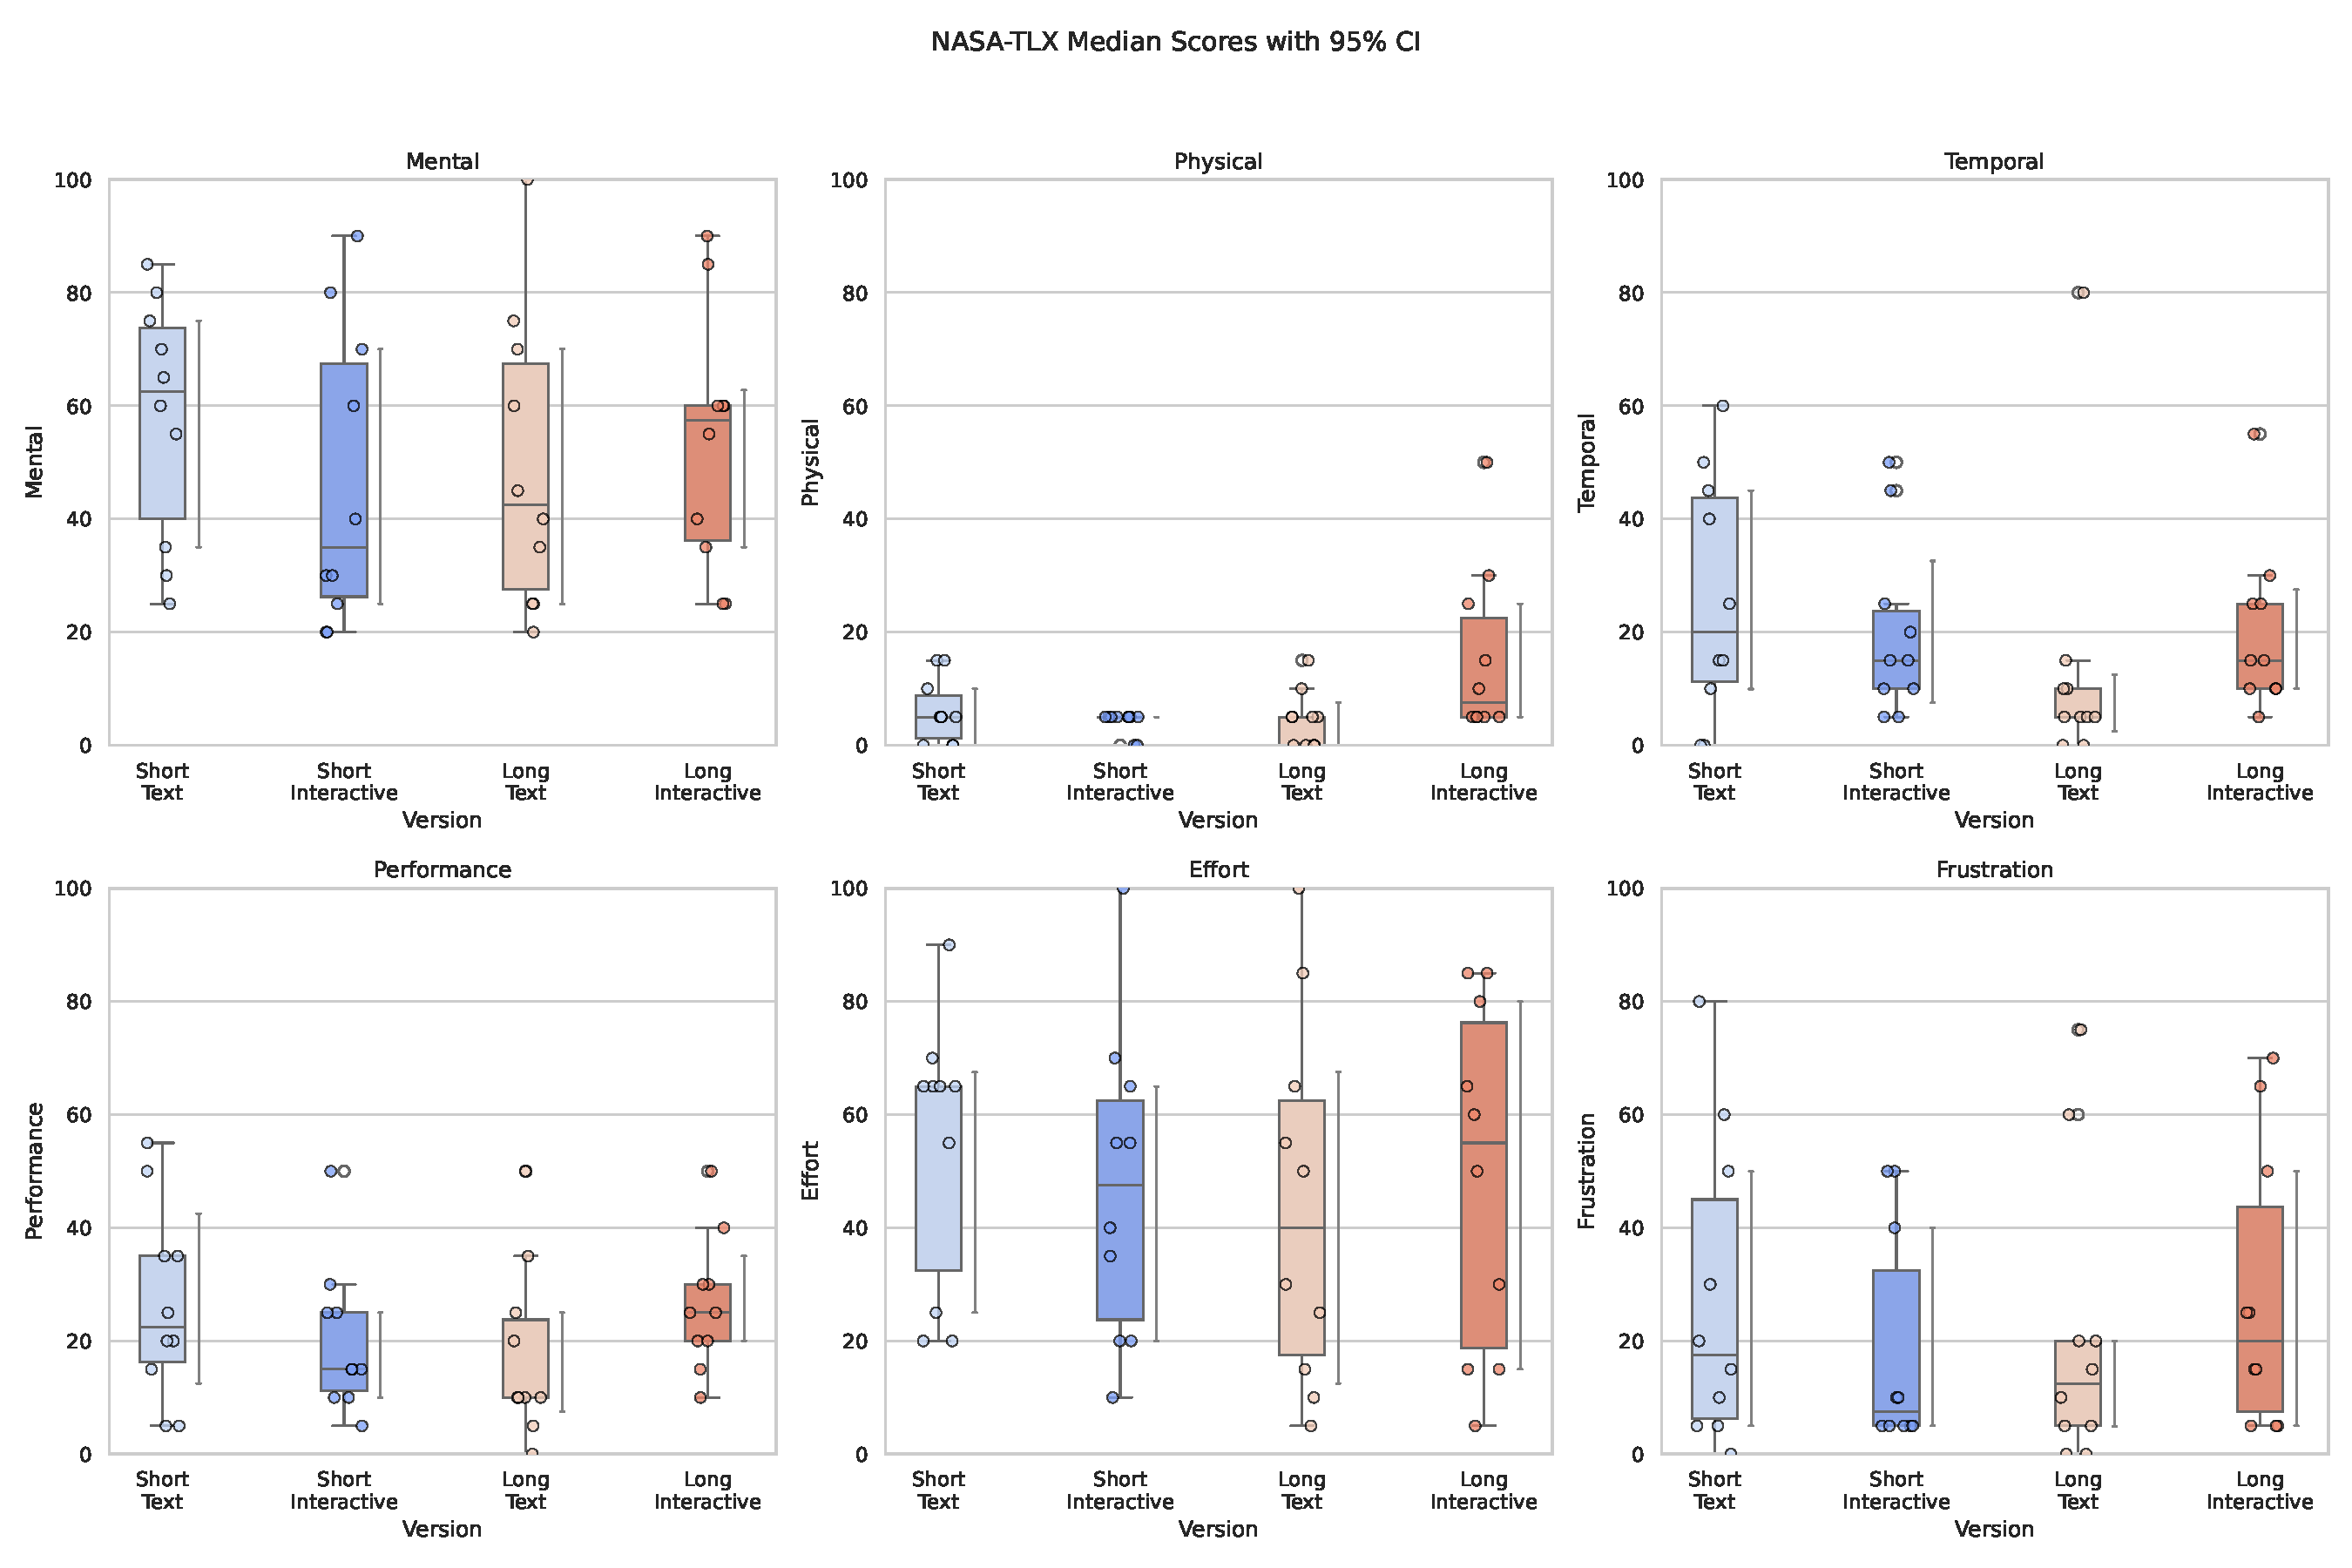
\includegraphics[width=\textwidth]{content/image/results/nasatlx_final_value_with_CI.pdf}
    \caption{NASA-TLX Results}
    \label{fig:nasatlx-with-ci}
\end{figure}


\subsection{Sources of Cognitive load}
NASA-TLX consists of six weighted dimensions: mental demand, physical demand, temporal demand, performance, effort, and frustration. To better understand the sources of cognitive demand and answer RQ2b, we highlight qualitative similarities and differences across four experiment conditions. This is followed by descriptive statistics and participant survey findings.

We present the raw NASA-TLX scale results in Figure~\ref{fig:nasatlx-with-ci}. Next to each box plot, a line is present to denote the 95\% confidence interval around the mean for each boxplot.

\subsubsection{Mental Demand}
Mental demand refers to the extent of mental and perceptual activity required. From the interview results, we identified two major sources contributing to mental demand:~\textit{Budget management} and~\textit{Preference construction}. Despite all experiment groups sharing these themes, we notice a distinct difference in the scope of~\textit{Preference construction}, especially when comparing long text and interactive interfaces.

\paragraph{Budget management} $17$ participants expressed demand from trying to budget within limited credit ($N=4$), track remaining credits ($N=10$), and maximize the use of credits ($N=8$). For example:

\begin{displayquote}
How many I got left that~\ldots\ that I haven't voted on yet, and seeing if I and looking at the remaining credits, I'm trying to mentally divide that up before I start allocating upvotes and downvotes.

\small{\noindent \hfill -- S006, long interactive interface}
\end{displayquote}

\begin{displayquote}
And then I just wanted to make sure that I used all the credit that I had available to me, and also knowing that in order to like show your support for certain societal issues you had to like that was giving a tangential take away from other societal issues that you could support as well.
    
\noindent \hfill -- S032, short text interface.
\end{displayquote}

In the first quote, the participant struggles with not running out of credit while allocating credits to options they haven't yet attributed. The second quote highlights the challenge of maximizing spend while ensuring sufficient differentiation. All these factors relate to effective budget management.

\paragraph{Preference construction} Almost all participants ($N=36$) experienced an increase in mental demand due to preference construction. This can be broken down into three sources: determining relative preference ($N=16$), where participants focus on internal evaluation and comparison among different options; option prioritization ($N=17$),  where participants make trade-offs to identify high-priority options and translate internal preferences into a subset of options; and precise resource allocation ($N=30$), where participants allocate specific values or adjustments to represent their preferences. For each of these sources, we show an example:

\begin{displayquote}
Figuring out my priorities, and how much I prioritize option 1 over option 2. What is the difference between those 2 on my priority list?

\hfill -- S002, short interactive interface, determining relative preference
\end{displayquote}

% I think the whole time I was trying to balance, I think II think I partly was discovering my what's the word I want to use bias isn't quite right. My priorities (S031, I)

\begin{displayquote}
I knew which ones that I wanted to dedicate the most to, and I knew which one I wanted to dedicate the least to. But it was that middle area that was kind of a grey area.
    
\noindent \hfill -- S008, short interactive interface, option prioritization
\end{displayquote}

% I knew which ones that I wanted to dedicate the most to, and I knew which one I wanted to dedicate the least to. But it was that middle area that was kind of a grey area.
% \noindent \hfill -- S024, short text interface, option prioritization

\begin{displayquote}
I'm not sure how to put into words~\ldots like having to pick how many upvotes would go to each one
    
\noindent \hfill -- S023, long text interface, precice resource allocation
\end{displayquote}

While these sources are common across all experiment groups, when we focus on participants in the long QS condition, the sources of preference construction showed different scopes between participants using text and interactive interfaces. More specifically, participants ($N=8$) in the long text interface tend to experience mental demand from preference construction by thinking about issues more narrowly and focusing on personal relevance. Conversely, participants ($N=9$) in the long interactive interface experience higher mental demand from considering the broader societal impact and evaluating options more holistically. Only four participants in the long text interface expressed a holistic view, and three participants in the long interactive interface expressed a narrow and personal view.

% \begin{displayquote}
% \bracketellipsis also seeing the long list and obviously having to pick between quite a few things that I do feel very strongly about and having to figure out which ones do, I feel more strongly about than others.
    
% \noindent \hfill -- S023, long text interface
% \end{displayquote}

\begin{displayquote}
Trying to figure out what upvotes I should give it you know~\ldots compared to~\ldots I even kind of went back compared to the other topics: <topic one> compared to <topic two>, and even with like <topic three>, I kind of went back and forth between those two. \bracketellipsis So it was very mental tasking for me.

\noindent \hfill -- S015, long text interface
\end{displayquote}

% \begin{displayquote}
% \bracketellipsis really having to think, especially with so many different societal issues. How do I personally prioritize them? And to what extent do I prioritize them?
    
% \noindent \hfill -- S009, long interactive interface
% \end{displayquote}

\begin{displayquote}
\bracketellipsis really going through the rest of the categories and deciding okay, which are the pressing issues of our time and which are the pressing issues for this particular society that that I live in. \bracketellipsis You know these causes need a lot more funding, and and others can probably still have some sort of an impact, even with less resources.

\noindent \hfill -- S019, long interactive interface
\end{displayquote}

In the first quote, participants expressed mental demand narrowly focused on three options, trying to recall specific characteristics to differentiate among the options. In the second quote, participants consider how options play a role in society and the bigger picture, aiming to maximize impact. While these differences seem subtle, they indicate a shift in cognitive load. It is possible that exposing participants to all options during the organizing phase forced them to think through all options.

Circling back to mental demand related to budget management across these two experiment conditions, we find that long text interface participants focused on more operational behaviors such as:

\begin{displayquote}
So I wanted to be fair.~\bracketellipsis I actually took my calculator out and said~\bracketellipsis  how much would it be if I equally distributed it and then how do I do that? Do I wanna do it all equally or not?

\noindent \hfill -- S020, long text interface
\end{displayquote}

compared to more procedures involving more strategic planning such as:

\begin{displayquote}
I wanted to make sure I wanted to give some credit to everything~\bracketellipsis I'm trying to make sure that I had without doing a lot of~\ldots I guess redos is trying to kind of get it right the first time on how I weight things.

\noindent \hfill -- S032, long interactive interface
\end{displayquote}

Strategic planning does not refer to gaming out others or 'winning' a game but rather to high-level thinking processes that consider strategies and plans to tackle a challenge, compared to operational tasks such as adjusting a specific vote value. While we did not notice significant differences in mental demand raw values (Figure~\ref{fig:nasatlx-with-ci}, top left figure) across the four experiment groups, the different actions regarding budget management and preference construction show a shift in mental demand across experiment conditions.

% IN_T4: Wanting more information on the options (N=6/40)
% 5. While the numbers seem small, non of this request came from v3. This could explain that participants are already overloaded from the existing the task.

% ============================================= %
\subsubsection{Physical Demand} Physical demand refers to the physical effort required to complete a task, such as physical exertion or movement. Since this study involves participants sitting in front of a computer screen completing a survey, most participants reported minimal physical demand. We nonetheless report the sources of this minimal demand, which include reading text on the screen ($N=4$), using the mouse ($N=16$), and moving their head to navigate the vertical screen ($N=5$). Participants emphasized that these demands were minimal, which is reflected in the low values reported in the NASA-TLX physical demand scores (Figure~\ref{fig:nasatlx-with-ci} middle top image.)
Notably, $11$ out of $20$ participants that used the interactive interface mentioned physical demand from using the mouse, reflecting their increased interaction with the interface. This is further supported by the raw NASA-TLX physical demand scores, which show statistical significance between short and long interactive interfaces ($p<0.01$) as well as between text and interactive interfaces in long surveys ($p<0.05$) after running a Mann-Whitney U test.

% ============================================= %
\subsubsection{Temporal Demand}
Temporal demand refers to the time pressure felt by the participant while performing a task. A lower temporal demand suggests participants experience a slow and leisurely pace.

The themes we uncovered from the interviews consist of three main sources that lead to participants' increase in temporal demand. These include:~\textit{Budget}, ~\textit{Decision Complexity}, and ~\textit{Operational Efficiency}. 

\paragraph{Budget}
Budget is a lightly discussed theme that emerged across experiment conditions. Four participants mentioned budget increasing their temporal demand. Although budget can only decrease through spending, it is interesting that some participants expressed that the reduction in credit value created a sense of time pressure. Participants translated the increasing marginal cost of votes into higher temporal demand. As one participant said,

\begin{displayquote}
When the money was decreasing, as I was casting more upvotes or downvotes so as the money decreases I felt kind of rushed.
            
\noindent \hfill -- S034, long interactive interface
\end{displayquote}

\paragraph{Decision Complexity} Decision Complexity refers to when participants felt that there are many decisions to make. These causes are expressed in two forms—affirmative and negative. Affirmative perception refers to participants explicitly expressing that there are many decisions to make, while negative perception refers to participants describing concerns regarding the time and effort already invested in the survey.

\begin{displayquote}
So it didn't take too much time but obviously there was a lot of things to consider. So there was some temporal demand.
    
\noindent \hfill -- S022, short interactive interface
\end{displayquote}

\begin{displayquote}
\bracketellipsis so at first it was like, `Okay, this is fine.' But then on the end, I was like, maybe I should just hurry up and make a decision. So it's like at first it would been here, but then I kinda moved up near the end when I was hanging a waffling between my upvotes.
\noindent \hfill -- S024, short text interface
\end{displayquote}

The former quote pointed out participants making many decisions , while the latter highlighted the increase in temporal demand due to an expected devoted time. What we found important was that each experiment group had participants expressing both perspectives on decision complexity as a source of temporal demand. However, half of the participants ($N=5$) in the short text interface and half of the participants ($N=5$) in long interactive interface expressed concerns due to decision complexity. The long interactive interface involved all five participants registering an affirmative perspective. This is not surprising because participants in the long interactive interface had the most actions needed for organizing and voting. On the other hand, it is interesting to observe that four of these five participants in the short text interface expressed a negative perspective. This indicates that participants in this group are highly sensitive to their sunk cost effect.
% v2 -- 2 and v3 -- 3

\paragraph{Operational Efficiency}
Unlike decision complexity, which refers to the abundance of decisions to be made, operational efficiency refers to specific and concrete operations or goals. For example, completing the survey, executing an operation, or accomplishing a specific task like updating vote values.

\begin{displayquote}
I wanna get through things in an efficient manner which doesn't necessarily mean I rush it. But it does mean that I do things expeditiously. Especially. I'd like to think I'm somewhat computer-savvy. And so to be able to move through this quickly and efficiently. I do take pride in, but it's all personal stuff. It's not nothing outwardly influencing me. 
        
\noindent \hfill -- S032, short text interface
\end{displayquote}

\begin{displayquote}
I want the credit done but I don't want to be overthinking.
            
\noindent \hfill -- S013, short text interface
\end{displayquote}

The former quote refers to the participant aims to operate swiftly on the interface, not specifically related to decision making. Similarly, the latter focuses on using the credit to complete a specific goal. When asked about temporal demand, 11 participants (five from interactive and six from text interface) out of 20 who responded to the short survey expressed operational efficiency resulting in temporal demand, compared to just five (three from text and two from interactive interface) out of 20 in the long interface group.

Taking~\textit{Decision Complexity} and~\textit{Operational Efficiency} altogether, we interpret that the participants in the short survey misperceived the task as simple, seeing just six options on the screen, and thus anticipated the task to be simple and easily completed. We observe similar patterns from the NASA-TLX temporal demand raw values (Figure~\ref{fig:nasatlx-with-ci}). The short text interface shows a relatively higher demand across the four groups, reflecting the demand from both decision complexity and operational efficiency. This is followed by the short interactive interface, affected by operational efficiency, and the long interactive interface, affected by decision complexity. The long text interface showed the least amount of temporal demand. Our statistical tests showed a significant difference between the long text interface and the long interactive interface ($p<0.05$) after a Mann-Whitney U test.

It is also worth noting that three participants from the 20 who responded to the long survey mentioned that the vertical screen's ability to see all options facilitated direct comparisons and transparency about the entirety of the task, which reduced the temporal demand.

\begin{displayquote}
(Seeing) all at once I can see how many there are, so it's kind of like I can kind of tell when I will be done.

\noindent \hfill -- S041, long text interface
\end{displayquote}

% ============================================= %
\subsubsection{Performance}
Performance refers to how the person perceived if they successfully completed the task. A lower value refers to a good performance and vice versa. We find less differences between experiment groups qualitatively and quantitatively. However, there are notable takeaways that we can derive from the data.

First, we identified two sources of performance demand:~\textit{Operational Actions} and~\textit{Social Responsibility} from the interviews. 

\paragraph{Operational Actions}
Similar to previous demands, operational actions refer to specific and executable procedures participants can perform in the survey. These sources are shared across experiment groups. Six participants reported feeling pressured to spend all their credits or ensure they stayed within budget. Five participants were concerned that their choices did not accurately reflect their true preferences. Additionally, six participants mentioned experiencing performance demand due to the limited time, energy, and resources available, which ties into other cognitive demands. Here we show two examples:

\begin{displayquote}
I don't think I did it perfectly, because I didn't have 0 remaining credits.
    
\noindent \hfill -- S024, short text interface, budget management
\end{displayquote}

\begin{displayquote}
I'm concerned that it's not as reflective of my views as I wanted to be like, or I was concerned about it.~\bracketellipsis I was concerned that maybe it didn't.

\noindent \hfill -- S041, long text interface, preference reflectiveness
\end{displayquote}

\paragraph{Social Responsibility}
Social Responsibility is a noteworthy source of perforamce demand, categorized into accounting~\textit{decision-maker responsibility} (N=8) and from considering~\textit{uncertainity of the outcome} (N=3). The former refers to individuals feeling guilty because they weren't able to avoid because of specific tradeoffs or that they want to be fair. For example, 

\begin{displayquote}
I don't want people to think that I just like don't care about <ethnicity> people at all. I also don't think like government funding should go towards like religious organizations. You know what I mean. So I don't want somebody to think that like, I just don't care about <ethnicity> people.
    
\noindent \hfill -- S041, long text interface, decision-maker responsibility
\end{displayquote}

In this quote, the participant placed themselves inside the shoes of a member of the government, rather than a citizen expressing their own attitudes. This shift in roles introduced the perforamce demand, however, it demonstrated that QS shared decision maker's dilemma to individual survey respondents. This characteristic extends to the latter which further to the participants trying to forsee an outcome:

\begin{displayquote}
If I was actually running a government funding~\bracketellipsis I don't know how this (the survey results) might actually affect people. Some of these things might be unpopular or bad, or have outcomes that I didn't forsee.
    
\noindent \hfill -- S027, short interactive interface, uncertainity of the outcome
\end{displayquote}

Similar to the previous source, social responsibility is also shared across experiment groups. Considering the raw NASA-TLX scores(Figure~\ref{fig:nasatlx-with-ci}), participants expressed similar levels of perforamce score. This aligns with the interview results where most participants felt positive about their final submission. This result is expected because the task is designed to reflect their preferences, not to measure performance. We further analyzed the types of satisfactory statements regarding performance.


We identified three types of satisfactory statements regarding self reported performance:
\begin{itemize}
    \item \textit{Did their best} refers to statements where a participant stated they exhausted their maximum effort to complete the task.
    \item \textit{Feel good} efers to statements where a participant who expressed positive emotions or satisfaction about their performance or the outcome.
    \item \textit{Good enough} refers to statements where a participant acknowledged that their performance or the outcome was acceptable or satisfactory, but not necessarily perfect or the best possible.
\end{itemize}

We found approximately the same number of participants in each of the four experiment groups expressed \textit{Good enough}. Meanwhile, participants using the interactive interface across short and long groups had almost double the number of participants ($N=11$) who expressed \textit{Feel good} compared to the text interface ($N=6$). On the other hand, the text interface had slightly more participants ($N=5$) who expressed \textit{Did their best} compared to the interactive interface ($N=3$).

This result highlights a few important takeaways. First, participants from all experiment groups expressed satisficing behaviors (\textit{Good enough}) with no particular group reporting a higher frequency of this behavior. Second, participants using the text interface are experiencing challenges that make them feel they have to do their best to complete the task. Last, participants using the interactive interface are generally positive about their experience and the outcome.

% TODO: Need to check the reflective thinking part a bit. I **think** there are differences but it is unclear, need to go back to raw code.


% ============================================= %

\subsubsection{Effort}
Effort refers to the amount of work required to achieve a level of performance. It includes the intensity of both mental and physical resources expended during the task.

Similar to our analysis for mental demand, we code the source of effort into to major categories:~\textit{Operational Tasks} and~\textit{Strategic Planning}.

\paragraph{Operational Tasks} Similiar to performance, we focus on operational tasks that contributed to effort with a narrow focus including: navigating the interface, managing the budget at an operational scale (i.e., making sure not to run out of budget, making specific updates between two options), or translating an opinion to a quantifiable adjustment on the survey. These narrower low level operations involves taking effort to making updates or actions related to the interface itself. We show two examples associated with different aspects of operational tasks that influence precieved effort:

\begin{displayquote}
And then I wanted to bump up (an option) maybe to 4 or <option> to 5 and realize I couldn't. My point (number of votes) had to like back down a little bit~\ldots So that would be effort came in of how do I want to really rearrange this to make it (the budget spending) maximize?

\noindent \hfill -- S029, short text interface
\end{displayquote}

\begin{displayquote}
So it was like it was very~\ldots I have to put a lot of effort in terms of you know~\ldots think about each dimension that if I give one credit to <option name> whether it will affect my credits on <another option name>.

\noindent \hfill -- S005, long text interface
\end{displayquote}

Notably, $14$ of the $20$ participants using the text interface expressed overwhelminly mentioned sources related to such sources, compared to less than half of the participants ($N=7$) from the interactive interface, with the lowest mention by the long interactive interface group ($N=2$). We review the other category before making interpretations.

\paragraph{Strategic Planning} Opposite to operational tasks, strategic planning follow definitions established for mental demand which involces higher level strategies to complete the survey. We further derive two distinct types of planning:~\textit{personal} and~\textit{global}.~\textit{Personal strategic planning} refers to taking effort to translate preferences onto the survey without considering governing values or broader beliefs. For example, this participant expressed effort from retrieving past experiences to inform their decisions:

\begin{displayquote}
~\bracketellipsis having that prior experience and being able to quickly link it to a tangible thing that I've experienced in my personal life.

\noindent \hfill -- S032, short text interface
\end{displayquote}

\begin{displayquote}
And really the bulk of the effort was how to rank order these (options) and allocate the resources behind the upvotes so that I can accurately depict what I want~\ldots say, a committee to focus on and allocate actual fungible resources, too. 

\noindent \hfill -- S019, long interactive interface
\end{displayquote}

While the difference in the number of citations to personal strategic planning are less pronounced across groups, the interactive interface (N=13) still scores slightly higher counts compared to the text interface (N=9).~\textit{Global strategic planning}, on the other hand, involves participants formulating strategies to align with broader, communal values. This includes ensuring fairness, considering the impact of different options on the entire community, and evaluating the complex relationships between various options. For example:

\begin{displayquote}
I think, imagining the trying to imagine every outcome trying to to imagine what what else would be encompassed, encompassed by each category.

\noindent \hfill -- S027, short interactive interface
\end{displayquote}

\begin{displayquote}
Hey, even though I don't really like this idea. But what if they're important? They sort of kind of deserve some attention~\ldots that's why I think I have the effort here.

\noindent \hfill -- S037, long interactive interface
\end{displayquote}
    
Both examples shows considerations beyond personal experiences, considering outcomes or social values. We notice that nearly twice as many participants (N=7) in the interactive interface expressed effort from global strategic efforts compared to the text interface (N=4). Altogether, we observe more participants using the interactive interface (N=17) reported sources of strategic effort compared to those using text-based interfaces (N=11). 

Qualitative analysis in this subsubsection added clear evidence that the source of cognitive demand for effort differs between text and interactive interfaces, similiar to mental demand. Participants using the interactive interface focus less on operational tasks and more on strategic planning, specifcially global strategic planning, where they think about options holistically and beyond the option itself. This is in contrast to participants using the text interface, who focus more on operational tasks and a narrower strategic planning scope. The raw NASA-TLX effort scores (Figure~\ref{fig:nasatlx-with-ci}) can then be explained that even though reported values are similar across the four experiment groups, the sources of effort differ between text and interactive interfaces.

% ============================================= %

\subsubsection{Frustration}
Fustration is the last dimension of NASA-TLX. It refers to the extent to which the participant is annoyed, irritated, or discouraged during the task.

Following the previous analysis, we categorize the sources of frustration into three major themes:~\textit{Operational Actions} and~\textit{Strategic Planning}

\paragraph{Operational Actions} Similar to the previous definitions, $15$ participants highlighted this source for frustration. Six participants expressed frustration regarding credit management (i.e., overspending budget); four participants mentioned had trouble deciding the final value for the options; three participants are frustrated because they need to make multiple decisions; five participants were frustrated with the quadratic mechanism; four participants are frustrated trying to understand the content of the option or how the option connects to them. For example, 

\begin{displayquote}
I was slightly frustrated when doing the task, probably because there was a budget that we kind of had to stick with it.

\noindent \hfill -- S001, long text interface, quadratic mechanism
\end{displayquote}

\begin{displayquote}
i think just frustration~\bracketellipsis because when i was making like the decisions on how many upvotes I could put in each section, I was running out of credits.

\noindent \hfill -- S013, short interactive interface, budget management
\end{displayquote}

These demonstrated participants frustration because they are hindered by not being able to complete specific operational actions or constraints presented by QS. What is noteable is that all experiment groups had almost half of the participants express operational frustration compared to only two participants from the long text interface group. It is not clear why they did not encounter similiar frustration.

\paragraph{Strategic Planning} For frustration, we further derived strategic planning into two types: ~\textit{lower-level} and~\textit{higher-level}. For the former, Four participants expressed conflict between their personal preferences and what they believe would be other people's preferences. Eight participants experienced conflict between making tradeoffs among a few options. For example:

\begin{displayquote}
Because I know that's important to other people. But it just doesn't to me.
    
\noindent \hfill -- S010, short interactive interface
\end{displayquote}

\begin{displayquote}
I would have loved to have given more to other groups~\ldots and I felt stressed like~\bracketellipsis well~\ldots it's a group that you know is still~\ldots you know~\ldots important~\bracketellipsis
\noindent \hfill -- S020, long text interface
\end{displayquote}

These quotes showed participants trying to ahere to lower-level strategies such as considering personal prefernces or making trade-offs within a smaller scope. Compare to~\textit{higher-level strategic planning}, where six participants expressed conflicts that touch on the broader society and their core values of looking at the broader scope. Eight participants felt frustrated because they were forced to make trade-offs among \textit{all} options instead of a few. For example,

\begin{displayquote}
I had to consider how I feel towards that~\ldots how religious media broadcasting is being used in like today's society~\ldots today's political environment. So yeah~\ldots you really have to consider what is important to you. 
\noindent \hfill -- S020, long text interface, value conflicts
\end{displayquote}

\begin{displayquote}
I think the frustration is~\ldots I wish that we could help all of these causes, but you know it's just like anything else. You can't do everything and when it's not~\ldots  I feel like it's hard to quantify how much some of these things should be supported versus others. So when you're talking about upvotes and things that's challenging to me, it's frustrating.
\noindent \hfill -- S026, long interactive interface, considering all options
\end{displayquote}

Fustration that stemmed from strategy planning are spread across all experimental conditions. Reflecting on the raw NASA-TLX scores (Figure~\ref{fig:nasatlx-with-ci}), We only see a slight difference in less frustration from the long text interface participants compared with the rest of the participants, likey due to the less frustration from operational tasks. Thus, we interpret that frustration comes more from individual's ability to discern and make decisions and not necessarily tied to specific methods in the construction of preference.

\subsubsection{Summary}
% TODO: make a table
To recap, the analysis identified the different sources of cognitive load experienced by participants. More specifically, it highlighted differences across experimental conditions. Interactive interfaces, especially long ones, drive participants to adopt a holistic view and encourage higher-level deliberation, indicated by increased mental demand and effort. Conversely, participants perceived more operational demand when completing specific tasks using the text interface. Mental demand, effort, and temporal demand highlighted the urgency participants felt to complete tasks swiftly. This distinction doesn't mean one group of participants excludes the other group's demands, but it highlights that the main source of demand shifts with different interfaces.

% ============================================= %
\afterpage{
\begin{landscape}
    \begin{figure}[ht]
        \centering
        \begin{subfigure}[b]{0.26\pdfpageheight}
            \centering
            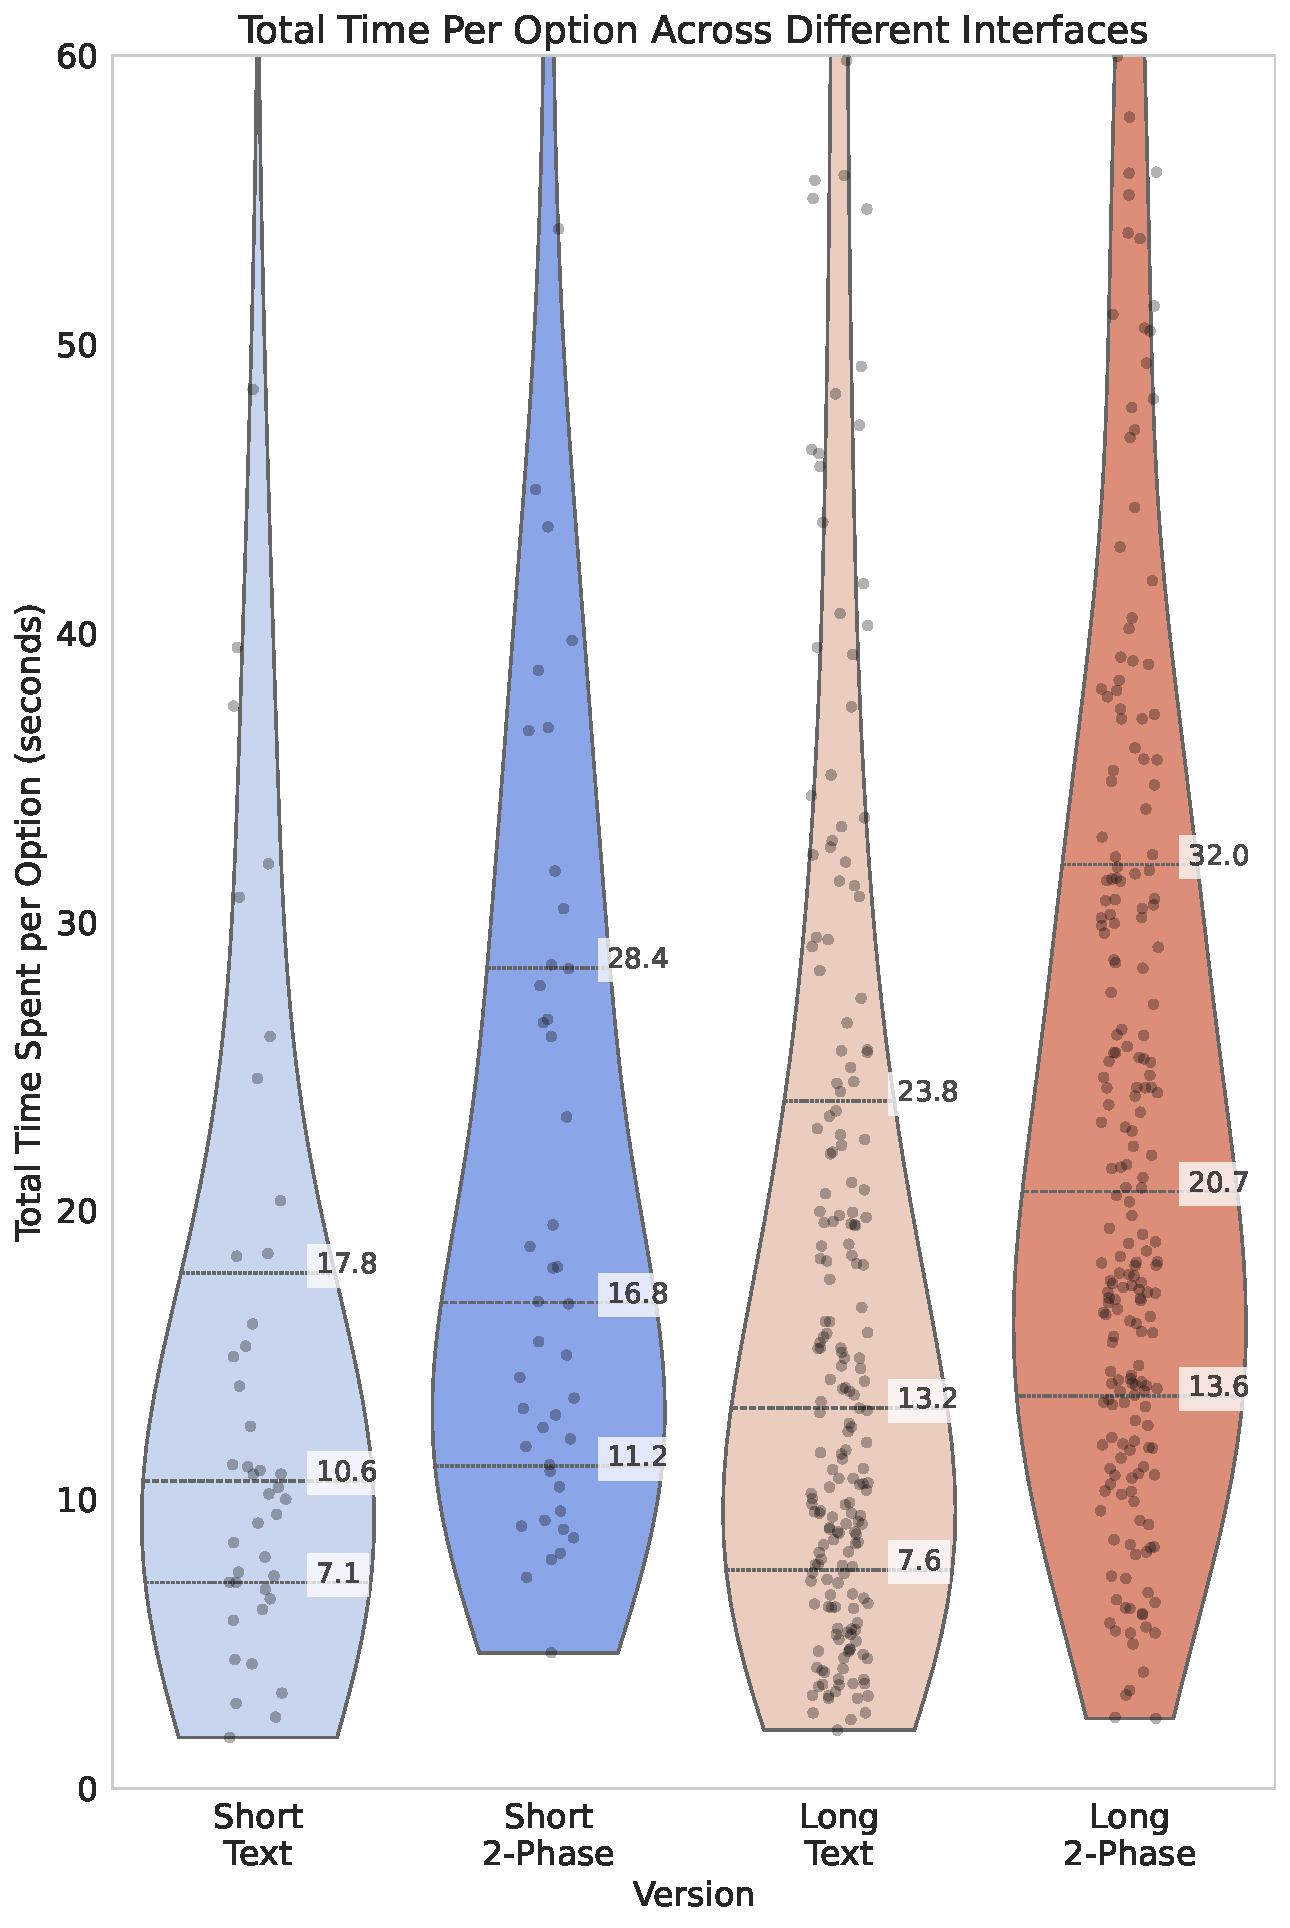
\includegraphics[width=\textwidth]{content/image/results/total_time_per_option.pdf}
            \caption{Total Time per option}
            \label{fig:total_time}
        \end{subfigure}
        \hfill
        \begin{subfigure}[b]{0.26\pdfpageheight}
            \centering
            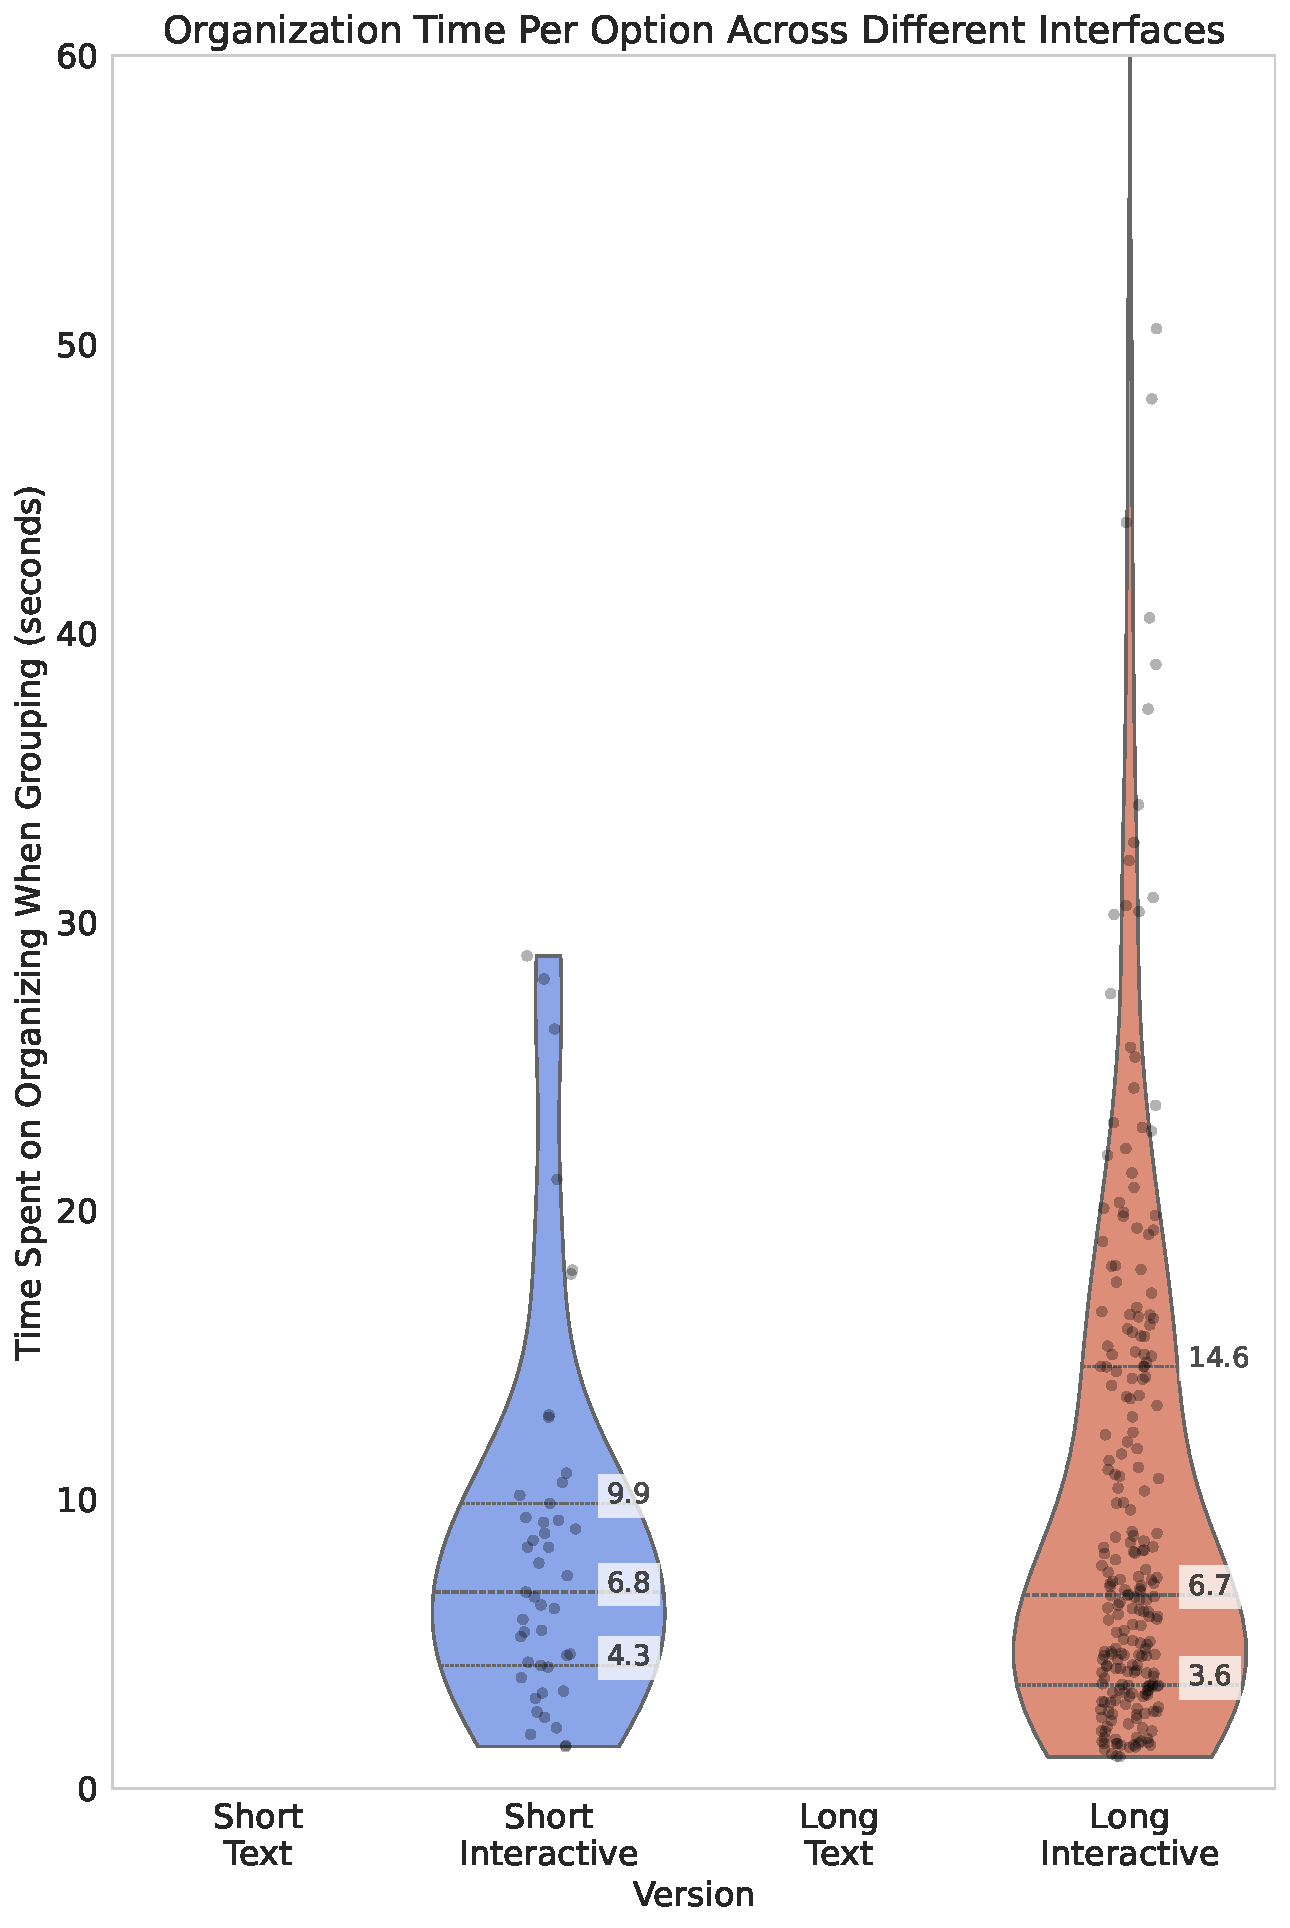
\includegraphics[width=\textwidth]{content/image/results/org_time_per_option.pdf}
            \caption{Organization Time per option}
            \label{fig:org_time}
        \end{subfigure}
        \hfill
        \begin{subfigure}[b]{0.26\pdfpageheight}
            \centering
            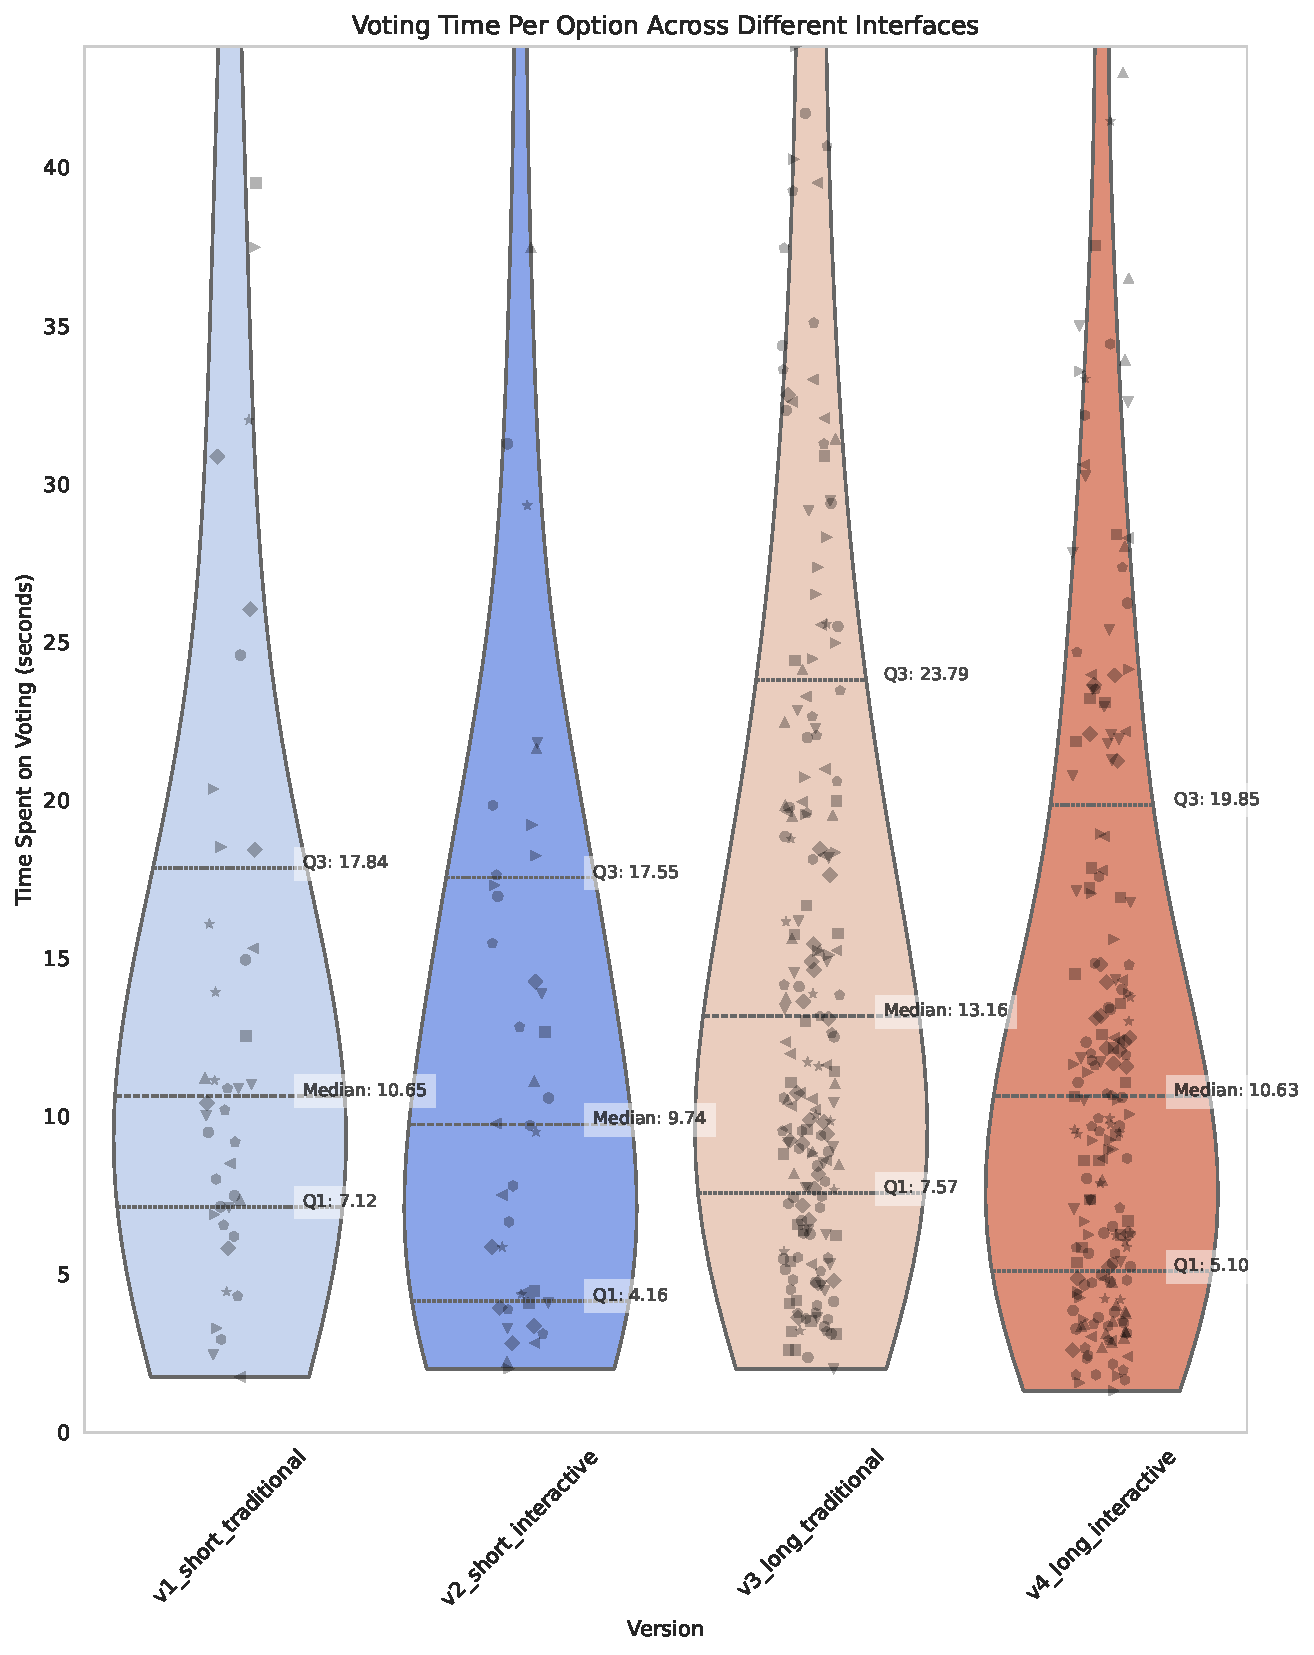
\includegraphics[width=\textwidth]{content/image/results/voting_time_per_option.pdf}
            \caption{Voting Time per option}
            \label{fig:vote_time}
        \end{subfigure}
        \caption{Breakdown of time per option}
        \label{fig:Time Spent Per Option Per Person}
    \end{figure}
\end{landscape}
}

\subsection{Interaction Behavior Analysis}
\label{sec:act}
To answer RQ3 and collect evidence of shifts in participants' cognitive sources, we analyze their behaviors during the survey. We aim to understand the time participants spend on options and when they make changes. When a participant clicks their mouse on the interface to complete an action, such as drag-and-drop, updating votes, or placing options into a specific group, a timestamp and the payload of the update are stored in the log. In this subsection, we analyze these log data. We acknowledge that the time difference between two actions indicates the time the participant took to decide and act. Although participants might be thinking about other things, this is our best proxy to study their behaviors.



\subsection{Time Spent per Options}
First, we define time spent per option. A participant can enact several actions related to the same option, for example, a participant might spend $t_1$ time to place the option into a `lean positive' category; spend $t_2$ and $t_3$ time to drag and drop the options to reposition it on the interactive interface; spend $t_4$ and $t_5$ time to update the upvotes on that option. In this case, we would define voting time as $t_4 + t_5$ for that option, and organization time as $t_1 + t_2 + t_3$.

To reduce noise, we intentionally drop all the time participants spent on the first option in the organization phase or voting phase. The goal is to reduce the inclusion of time they spent on reading the prompt, forming their preference, or understanding the interface. We present the results in Figure~\ref{fig:Time Spent Per Option Per Person} where each of the dots represents the time accumulated for an option that a participant interacted with. The violin plot shows the distribution of the dots and the three horizontal lines represent the median, 25th percentile, and 75th percentile of the time spent for that interface.

In Figure~\ref{fig:total_time}, we observe that participants spent more time on the interactive interface than the text interface in both short and long surveys. A non-parametric statistical test supports such observation with $p<0.01$ for short and $p<0.0001$ for long surveys. This is not surprising because participants need to review the options and organize them in the interactive interface which takes more time. We break down the total time spent into organization time and voting time in Figure~\ref{fig:org_time} and Figure~\ref{fig:vote_time}.

Once we separate the organization time (Figure~\ref{fig:org_time}) and identify the voting time (Figure~\ref{fig:vote_time}), while there are no statistically significant differences between the text interface and the interactive interface in the short survey, we see a statistically significant reduction ($p<0.01$) in voting time between the text interface and the interactive interface. In other words, our original hypothesis holds in which the two-step design process did facilitate participants in making their decisions.

\begin{figure}[ht]
    \centering
    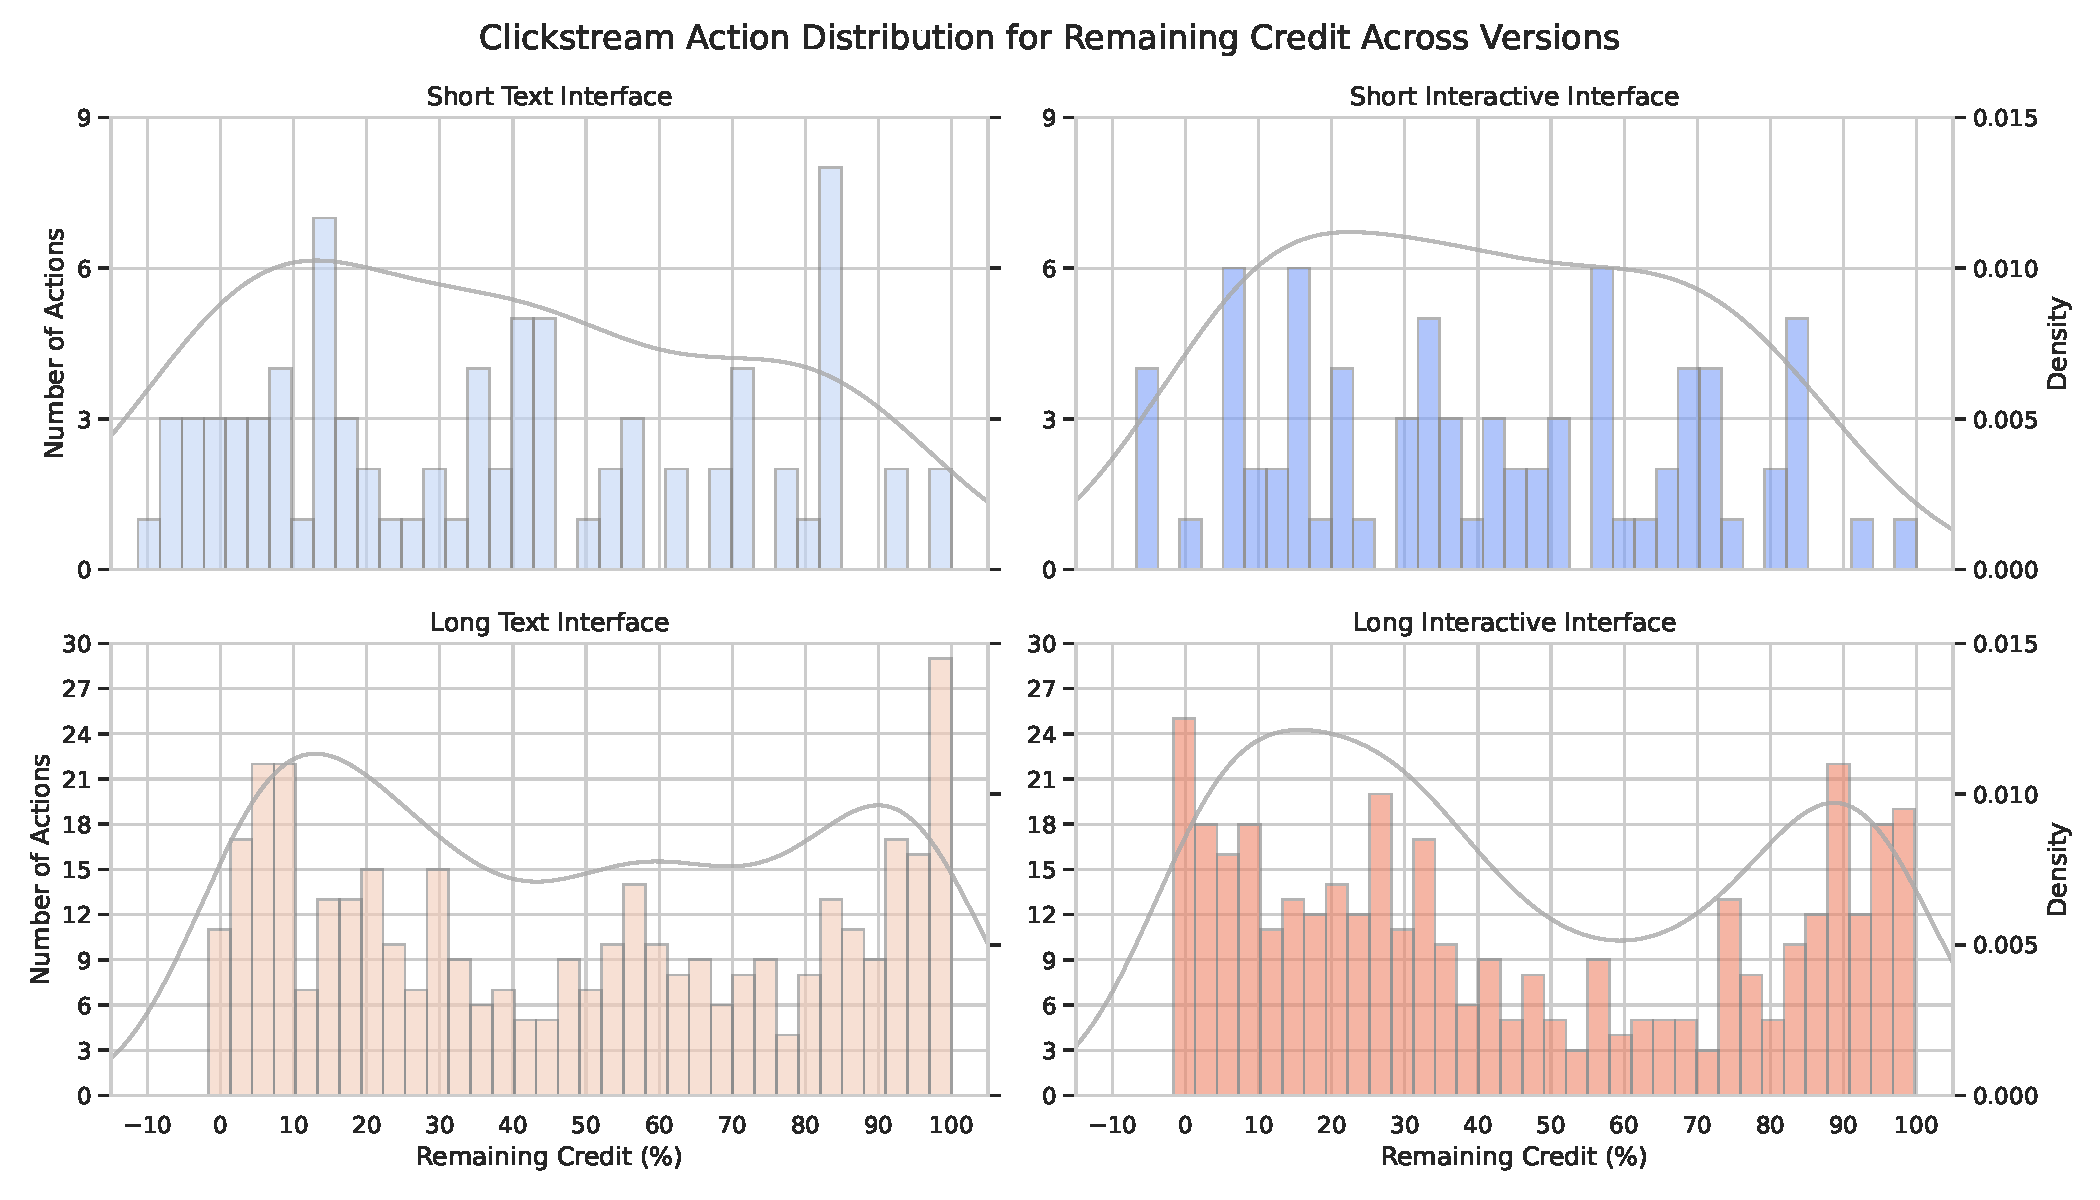
\includegraphics[width=\textwidth]{content/image/results/clickstream_action_distribution.pdf}
    \caption{voting actions across all options (needs to update chart text, remove normalization, and change the dot colors.)}
    \label{fig:voting_all}
\end{figure}

\subsection{Budget and Voting Behaviors}
Next, we examine participants' voting behavior and how it changed throughout the progress. Given that we observe significant differences in voting time changes comparing text interface and interactive interface for the long option survey, we focus on deciphering the voting action changes between these two experiment conditions in this subsection.

Figure~\ref{fig:voting_all} plots the time of voting actions over the remainder of the participant's budget across the text and interactive interface across all four groups. In other words, different from~\textcite{quarfoot2017quadratic} focusing on the number of accumulated votes over an individual's time, where they showed QV voters make more revisions than Likert Surveys, we focused on the budget scarcity which can influence QS respondents' behaviors.

In this plot, we see two distinct patterns between the short survey and the long survey in terms of participant behaviors. Only in the long surveys did participants exhibit more actions when the budget was abundant and when it began to run out, with the long interactive interface being more significant.

\begin{figure}[ht]
    \centering
    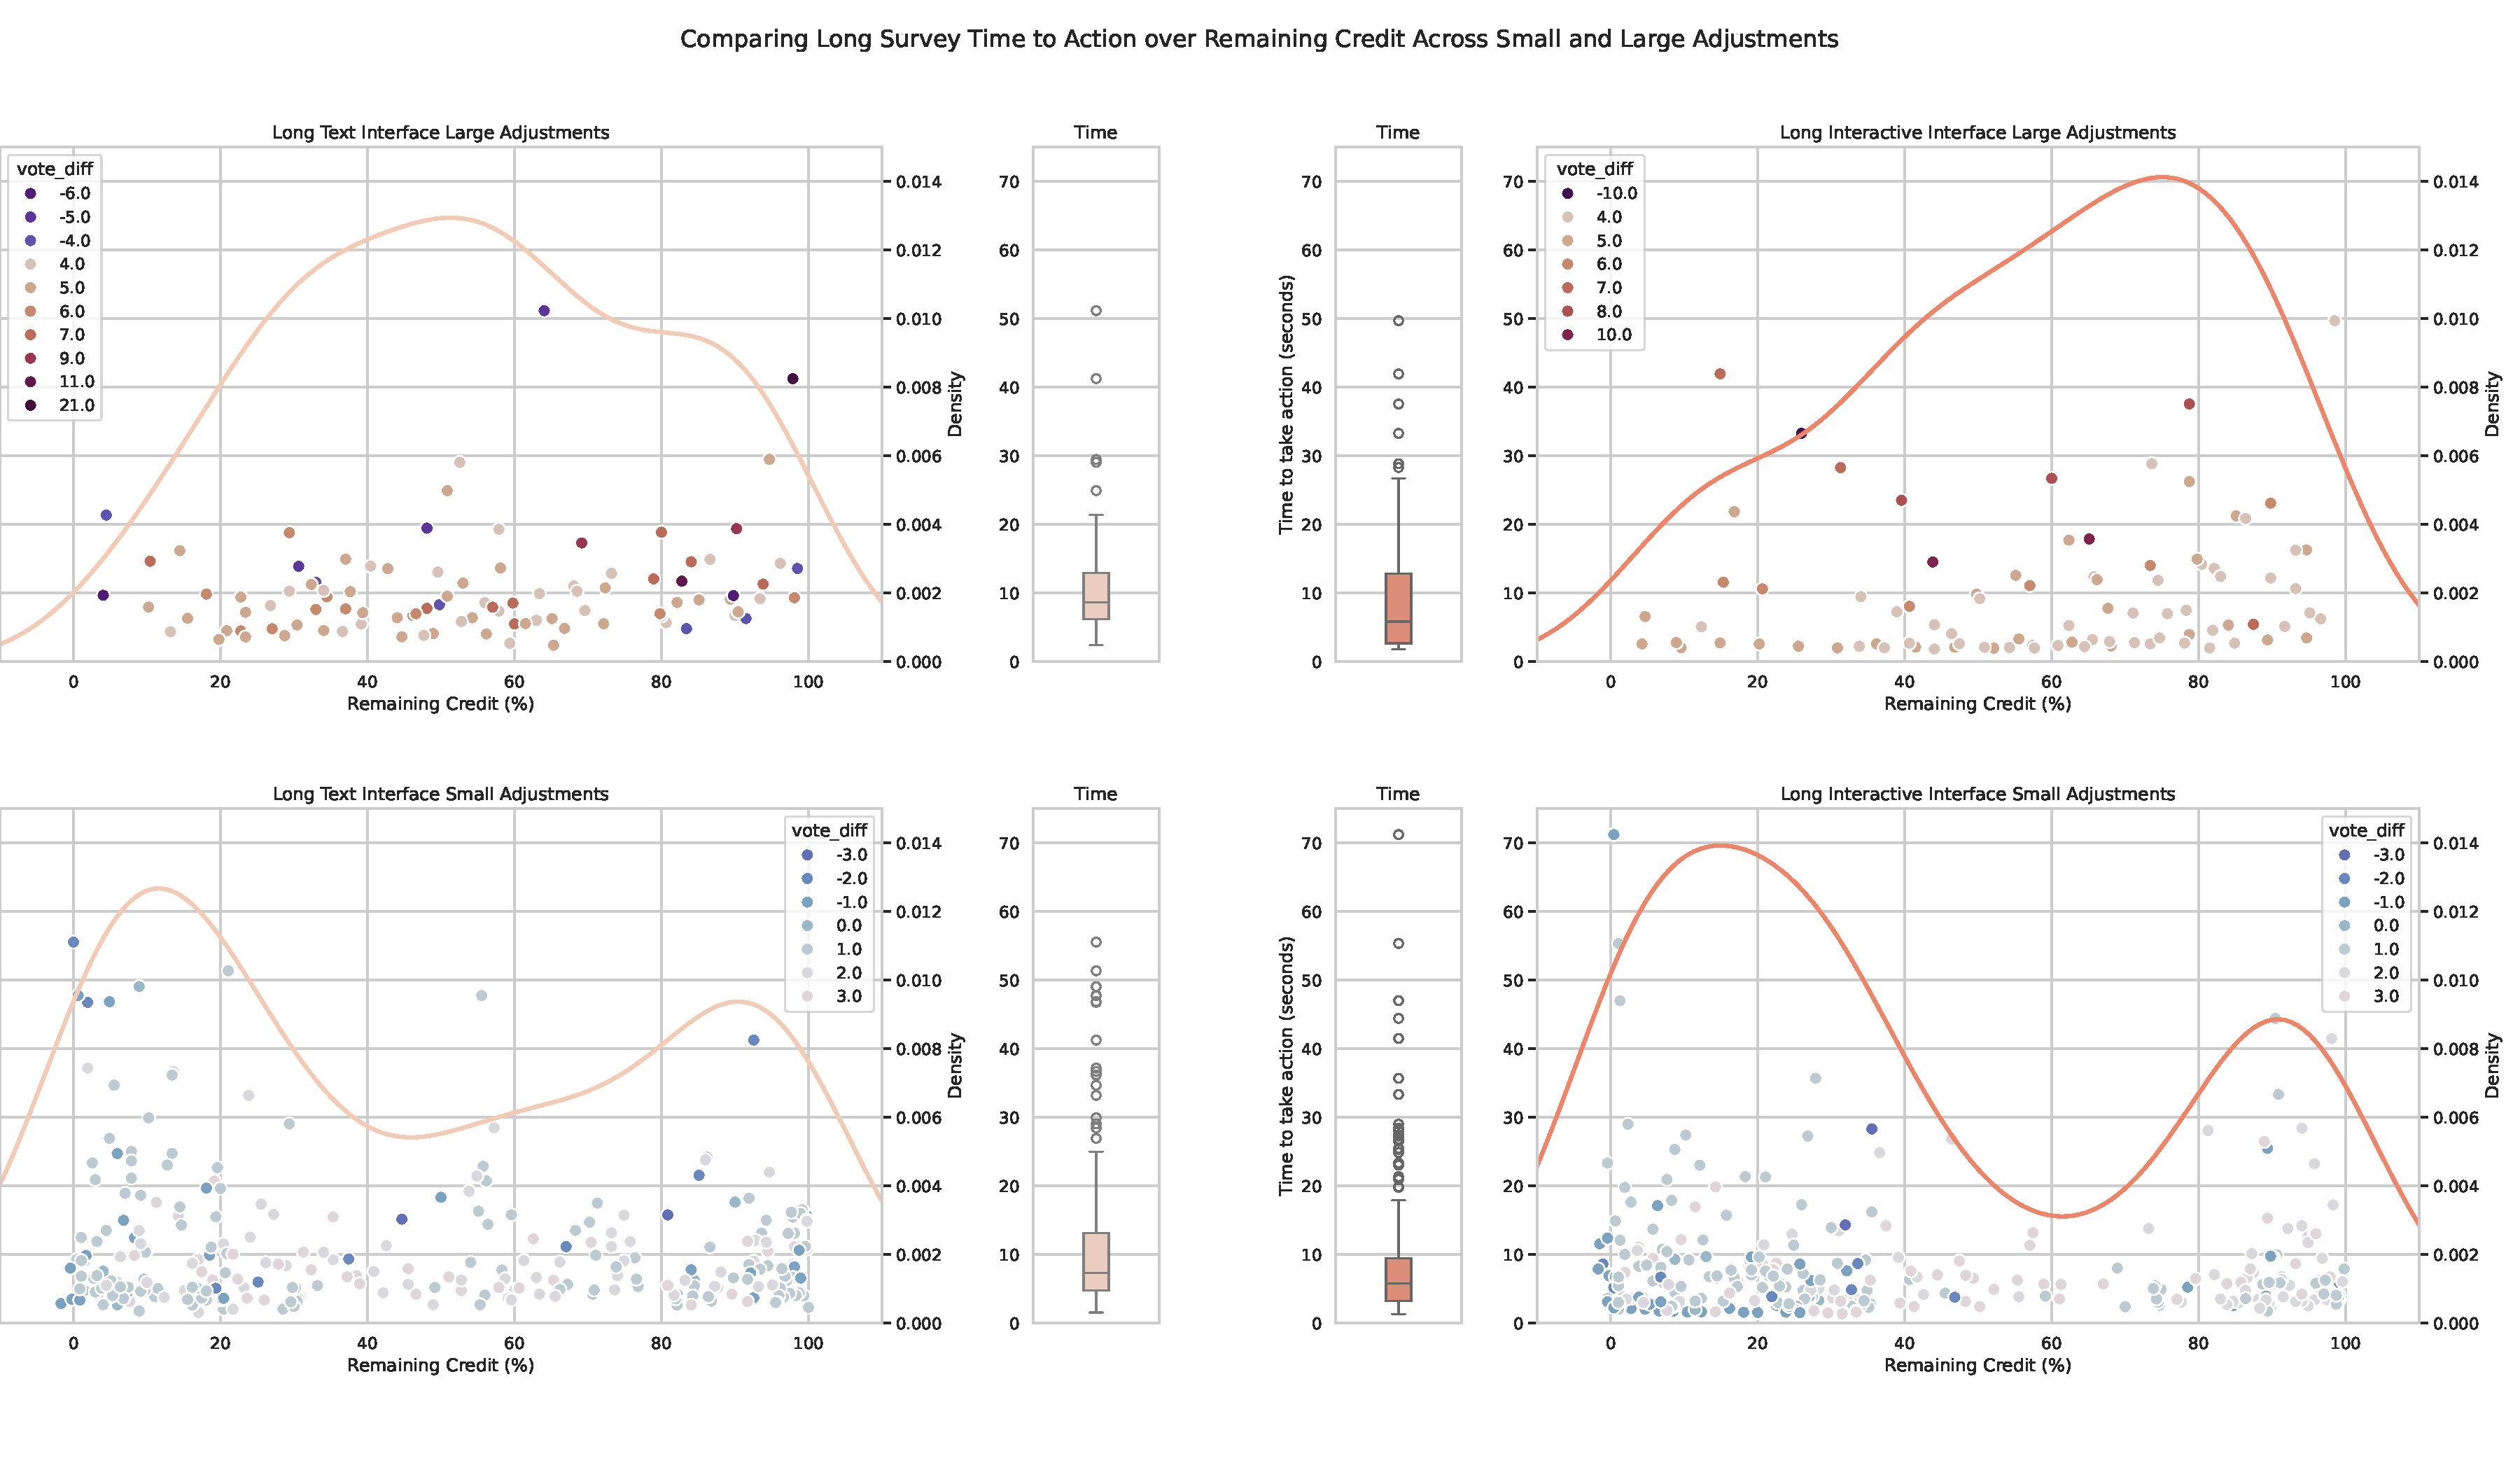
\includegraphics[width=\textwidth]{content/image/results/combined_density_plots.pdf}
    \caption{Breakdown of voting actions (needs to update chart text)}
    \label{fig:voting_v3_v4}
\end{figure}

Thus, we further separated the behaviors where participants made bigger changes or smaller changes to the option, specifically for the long version. In Figure~\ref{fig:voting_v3_v4} , we define an adjustment of four or more votes as a large adjustment which we plotted in the first row of the Figure. Adjustments of three or fewer votes are considered small adjustments.

First, we are able to surface the bimodal action distribution in both plots, with a even stronger signal for long interactive interface participants. Second, the plot demonstrated a clear cluster of voting actions in the bottom left corner of the interactive interface for small vote adjustments. In other words, participants made much smaller but more rapid adjustments when their budgets were running low. Second, larger adjustments are made when the participants have more options comparing the two plots on the first row. We interpret this behavior as participants in the interactive interface have constructed a clearer image of option preferences and, hence, have the ability to take larger strides in allotting their budget and deciding the number of votes at the beginning of the survey. Toward the end, participants using the interactive interface are then making fine-tuned adjustments to ensure that their preferences are reflected in their submissions.

% add qualitative support
\paragraph{Iterative Support from Interactive Interface}
Among all the interviews, when discussing about their experience of the interface, five particpants pointed out the importance of flexibility on the interface and how they took an incremental and iterative approach to navigating their attitude expression. All these participants are using the interactive interface. While this does not mean the study participant using the text interface did not use an iterative approach, but this highlighted the interactive interface encouraged the participants to make iterative and incremental updates. As one participant pointed out:

\begin{displayquote}
I like the fact that it remembers everything that you know. If if you make a mistake, that you don't lose all the work that you've already done. so I think that's very important is that it's an iterative process.

\noindent \hfill -- S019, long interactive interface.
\end{displayquote}

% Ti-Chung Cheng: So what elements of the software interface do you dislike, or like the most, if any, when expressing your preferences on responding to societal issues?
% S009: Hmm! What I like the most actually, probably the sorting function. I think that it really helped me organize my thoughts really, clearly, in terms of what I would dislike the most. really, not that much. I would say. yeah, also, like how we could categorize it, like even within the voting stage rather than just at the categorization stage. 

% Ti-Chung Cheng: Can you tell me a little bit more about the screen? How did the vertical screen help you?
% S037: I think because it helps the layout of, because it's like a long 3 bar. So it's easier for you to to drag and drop, and you can actually sort it, judging by the votes. But I do not do that. But I think this layout is could be helpful in that aspect.


\section{Discussion and Future Works}
\label{sec:discussion}
The goal of this study is to propose an interactive interface for QS and understand how the number of survey options, along with the interface, influences individuals' cognitive load and behaviors. Our results, presented in section~\ref{res:cog}, revealed that longer surveys did not increase cognitive load among participants. We further analyzed the sources of cognitive load and identified different causes across several dimensions. Participants using the interactive interface demonstrated more strategic planning and holistic thinking compared to those using the text-based interface, who focused more on operational tasks. Additionally, the behavioral analysis presented in section~\ref{res:act} showed that participants using the long interactive interface made more frequent, small, iterative updates, indicating a shift in their cognitive load focus.

In the discussion section, we address three key topics: first, we explore where participants experienced bounded rationality and how the current interface design supported decision-making. Next, we examine how participants constructed their preferences and how direct manipulation within the interface supported this process. Finally, we discuss how the interface design mitigated some challenges of quadratic mechanisms and identify remaining issues. Following these discussions, we provide recommendations for using this tool and propose design improvements for future development.

% ================================= %

\subsection{Bounded rationality and interface design}
One core repeated theme that emerged throughout participants' responses during the interview relates to bounded rationality. Bounded rationality defined by~\textcite{simonBehavioralModelRational1955} refers to the idea that individuals' cognitive limitations limited one's ability to use and process all available information, leading to a suboptimal resolution when decision making. When participants respond to a QS, they are faced with multiple options presented on the quadratic survey as well as the abundance of budget. Since the remaining budget translates to possible votes one can select to apply to an option, this adds additional numbers of decisions to make.

\begin{displayquote}
So I did say, Okay, you know, you thought of enough things, you know, and so it wasn't the most effort I could put in because again, that would have been diminishing returns. I tried to think of enough things that I could make, make a meaningful decision and then move on.

\noindent \hfill -- S036, short text interface.
\end{displayquote}

This quote exemplifies participants expressing their bounded rationality, trying to limit their effort to derive to their decision. Even though the drop-down menu showing all possible pre-calculated vote-credit values was a relief for a few participants so they do not need to search for the bounds, this sea of decision-making requires participants to recall and scramble information at once, which is extremely difficult. The byproduct of bounded rationality often translates to individuals satisficing behaviors~\cite{gigerenzerReasoningFastFrugal1996}, creating heuristics~\cite{tverskyJudgmentUncertaintyHeuristics1974}, over reliance on defaults~\cite{thalerNudgeImprovingDecisions2008a}, and problem decomposition~\cite{simonSciencesArtificial1996}.

Satisficing is the most common behavior observed among the participants, which refers to survey respondents making decisions that are not optimal but rather complete a 'good enough' decision. The same participant~\texttt{036} when asked about demand from performance then continues to describe:

\begin{displayquote}
I think that that's just not a realistic expectation (to be perfect), but I felt satisfied.~\bracketellipsis I felt like that (the response) was satisfied, but not perfect. Cause perfect is not a reality

\noindent \hfill -- S036, short text interface.
\end{displayquote}

Problem decomposition and dimension reduction are other common behaviors we observed. Several participants would create duo-dimension groupings, despite the experiment group they are in. Participants would have categories that cluster similar topics (i.e., all topics related to health vs. humanitarian) and categories that depict the positivity of their preference (i.e., positive vs. negative). Highlighting bounded rationality aims not to critique or exploit possible biases but to emphasize the importance of designing interface interventions to prevent survey respondents from making decisions that differ from their true preferences. For example, the design of showing one option at a time in the interactive interface lowers the possibility of participants being influenced by the default positions of options. One participant from the short text interface said:
\begin{displayquote}
Honestly, if medical research~\bracketellipsis I think if it was the first option, the first thing I saw, I probably would have given it more~\bracketellipsis because medical research~\bracketellipsis to me this seems like the most important, but I think if~\ldots if it was the first one I saw, I think it would automatically gave it a lot more.
    
\noindent \hfill -- S003, short text interface.
\end{displayquote}

% Another example comes from another participant from the long text interface. Recall that the options presented on the survey are randomly generated; even though there are some options related to the environment and education at the relevant location, participants were inferring the options to these topics. 
% \begin{displayquote}
% I think the categories were kind of in the same location. The environment stuff is at the bottom. Education policy is like in the top half. So I think I just looked and determined (my votes) that way.
    
% \noindent \hfill -- S035, long text interface.
% \end{displayquote}

The influence of bounded rationality highlights how critical and beneficial organization on the interface is. Many participants (N=7) who responded to QS using the interactive interface expressed the helpfulness of the organization phase proactively when asked what they liked about the interface in general. In fact, half of the participants (N=5) in the long interactive interface group expressed such an opinion. Multiple participants (N=4, 3 from the long interactive interface group) felt that the upfront introduction of all the topics allowed them to process and think about the full picture, thereby digesting all the information more comprehensively. 

\begin{displayquote}
I would say that (the interface) definitely (supported me), by being able to have a preliminary categorization of all the topics. First, it introduced me to all the topics, so that I can think about them like I can just kind of leave it there in my head space to think about and process \bracketellipsis So being able to digest all the information prior to actually allocating the budget or completing the quadratic survey.

\noindent \hfill -- S009, long interactive interface.
\end{displayquote}

Participants (N=4, 2 from the long interactive interface group) mentioned that organization support helped them to allot the intensity of votes by helping them focus and prioritize options through ranking. This exercise allows them to follow a clear decision-making process that avoids confusion.

\begin{displayquote}
If I had to choose a number like that in the beginning. That would have been really bad, but positive, neutral, negative. That was good enough.

\noindent \hfill -- S016, long interactive interface.
\end{displayquote}

\begin{displayquote}
I think \ldots\ ranking at the beginning one's impression towards these issues helps to like determine how many votes should be put towards them. 

\noindent \hfill -- S002, short interactive interface.
\end{displayquote}

Last, one participants highlighted the one-at-a-time approach during the organization phase allowed thoughtful reflection to think about their attitude toward that option.

\begin{displayquote}
Like, at the moment (during organization), when it gives you, like, rank it if it's positive or neutral or negative~\bracketellipsis it gives you time to just focus on that single thing and rank it based on how you feel at that moment.
    
    \noindent \hfill -- S013, short interactive interface.
\end{displayquote}

We also see a call for organizational features from participants using the text-based interface. Almost half of the participants (N=4) using the long text interface expressed a desire for features that can help reduce the decision space when responding to the QS.

\begin{displayquote}
If anything, I think I would like to be able to like, click and drag the categories themselves so I could maybe reorder them to like my priorities.

\noindent \hfill -- S025, long interactive interface.
\end{displayquote}

\begin{displayquote}
Because with this many (options), especially when I'm thinking \ldots\ Ok, where was (the option) \ldots\ Where was (the option) you know? Oh, that's right. Maybe I could give another up another upvote to the, you know whatever~\bracketellipsis

\noindent \hfill -- S028, long interactive interface.
\end{displayquote}

Active management of the options forced participants to think about their rough preference for each option at minimal cognitive requirements. The repositioning of options allowed participants to focus on subsets of the options during their decision-making process.

% ============================== %


\subsection{Construction of Preference on QS}
Since the interface supported some participants in managing their limited cognitive ability to make decisions, as shown in the previous subsection, we argue that the interactive interface \textit{shifted} the cognitive focus onto contributing to more in-depth preference construction and fine-tuning, even if it did not significantly reduce the cognitive load. Here we provide more evidence.

Literature from~\textcite{lichtensteinConstructionPreference2006} identifies three types of difficult decision-making scenarios: when one's preferences are not clearly defined, necessitating trade-offs, or quantifying opinions. We first show that participants constructed their preferences in situ. While some participants had existing preferences (e.g., environmental issues are important), they needed to reconsider aspects of the options or map them to their beliefs.

\begin{displayquote}

~\bracketellipsis the other part of the mental demanding was probably trying to associate with (what) I'm concerned in soci(ety)~\bracketellipsis is that question able to deal with my social concerns like, for example, climate change~\bracketellipsis How does that fit in?

\noindent \hfill -- S006, long interactive interface
\end{displayquote}

\begin{displayquote}

I mean, it's not necessarily a challenge, but it's interesting to see: `Oh, there are other aspects that I never care about.' And actually~\ldots some people care <an option>. Sure. Why? Why (should) I spend money on that? That's the first thought that comes to mind.

\noindent \hfill -- S037, long interactive interface
\end{displayquote}

Both quotes, one with a prior preference and the other without, illustrate how participants identified where the options on QS fall on their preference spectrum. Additionally, QS requires participants to utilize a common budget across options, necessitating trade-offs, as noted in prior works~\cite{chengCanShowWhat2021, naylor2017first}. Finally, selecting the final value involves quantifying opinions. Participants are thus engaged in a difficult~\textit{preference construction} decision-making process.

Behavior analysis in section~\ref{res:act} of participants using the long text and interactive interfaces revealed that they made small adjustments on the votes, clustered toward budget depiction with lesser time spent. These fine-grain adjustments indicated that participants are making less ad-hoc decisions; rather, they are deciding how to better utilize the remainder of the budget when the budget runs low. We identified a bi-modal interaction pattern.

We argue that the bimodal behavior observed in the voting actions across groups aligns with the Differentiation and Consolidation Theory presented by~\textcite{svensonDifferentiationConsolidationTheory1992} as we previously invisioned. Recall that the theory states that decision making contains a differentiation stage involving identifying differences and eliminating less favorable alternatives, while the consolidation stage strengthens commitment to the chosen option. In the interactive interface, we see a stronger bimodal indicating the two stages, compared to the text interface. As one participant mentioned:

\begin{displayquote}
I only start from the positive one~\bracketellipsis I finish everything~\ldots and then I move to the second part (the netural box).~\bracketellipsis I want to focus on these and make sure that resources are at least they get the attention they want. And if there's surplus and they can move to the second part

\noindent \hfill -- S037, long interactive interface
\end{displayquote}

These findings show the role of the two-phase interactive design in scaffolding the preference construction process. Additionally, several participants mentioned how the direct manipulation functionality, allowing individuals to drag and drop options for repositioning, supports their reflective thinking during preference construction. One participant noted:
\begin{displayquote}
So I tried to make a ranking \bracketellipsis and by creating this ranking, by dragging the related issues \ldots\ I don’t know \ldots\ that helped me organize my ideas.
\noindent \hfill -- S021, long interactive interface.
\end{displayquote}

\begin{displayquote}
I think the system was actually really helpful because I could just drag them. \bracketellipsis Because when I was unsure, because if I couldn't drag them then I couldn't compare 2 options very well like side to side, because this is a pretty long list \ldots\ so if I couldn't drag it, then I would have a harder time organizing my thoughts, whereas with the dragging feature I can really compare them, I can drag this one up here, and then compare it to the top one versus not being able to track it at all.
\noindent \hfill -- S039, long interactive interface.
\end{displayquote}

More importantly, it acts as a process for reflective verification and iterative decision-making. These can include post-reflection after expressing the intensity of preferences or preparation to decide on the number of votes for the next option.

\begin{displayquote}
So I would give the votes, and then I would drag and drop \bracketellipsis So I guess to see what my ranking looks like. And see if I could give more money or not.
\noindent \hfill -- S021, long interactive interface.
\end{displayquote}

\begin{displayquote}
\bracketellipsis this is something that's really important to me \ldots\ So I had the flexibility to move it to positive. So just having the kind of like shift in perception. \bracketellipsis especially because when I was doing categorization in the first step, \bracketellipsis what I thought about it in the moment. \bracketellipsis In the second step there was a shift in my perception of the issue just reflecting. So being able to change. That was really nice as well.
\noindent \hfill -- S009, long interactive interface.
\end{displayquote}

Conversely, in the text interface, one participant proactively mentioned a request to add click-and-drag functionalities to the interface. The participant described such function to group by topic categorization and also priority placement through direct manipulation.

\begin{displayquote}
If anything, I think I would like to be able to like, click and drag the categories themselves so I could maybe reorder them to like my priorities. And so I could maybe make that like a descending or ascending like list of like importance. \bracketellipsis if I could pull that up to the top, say myself like click and drag it up there, I think then I would stack the things I think it would affect under it. So like, I would put then, like youth, pro-education programs and adult education and early childhood programs and kinda stack those altogether. \bracketellipsis I would hope that money would trickle down and also increase all the rest of those things. So I would put less upvotes in there because I would hope to dribble out effect would kick in. \bracketellipsis I would kind of make myself categories and subcategories out of this list. If I could organize it.
\noindent \hfill -- S025, long text interface.
\end{displayquote}

Throughout the preference construction journey, we confirm that the two-stage interactive interface and the direct manipulation through drag-and-drop facilitated participants in constructing and reflecting on their preferences, adhering to preference construction theory.

% ========================= %

\subsection{Quadratic mechanism is challenging}
From the qualitatie interview, we found that many participants found automatic calculation critical. More than one-third of participants (N=14) from all four experiment conditions highlighted the importance of automated calculation from two perspectives: \textit{deriving cost} and \textit{keeping track of spent}. Two participants highlighted the importance of automated calculation regarding the cost for each vote.

\begin{displayquote}
I really like having the costs of all the votes displayed. When you select the dropdown menu and ranked in order.
\noindent \hfill -- S002, short interactive interface.
\end{displayquote}

Twelve participants highlighted the summarization box and the automated summation of the current credit spent, allowing them to focus on managing their next voting decision and expressing their preferences.

\begin{displayquote}
I thought I have \bracketellipsis (to) do all the numbers or calculation myself as a part of checking my ability of doing mathematics. But I guess you have taken care of that really well, so I could really really see that how much credit has left, and \bracketellipsis how well I should allocate \bracketellipsis I said that credit summary to be very specific. The credit summary section was really wonderful in doing all the calculation on that end.
\noindent \hfill -- S005, long text interface.
\end{displayquote}

\begin{displayquote}
I like that I don't have to make the calculation of the dollars that it does it automatically. So if I had to do it myself it would be more tedious. And so I think that that effort and frustration and mental demand would be much higher. So I appreciate that that calculation occurs automatically and very easily.
\noindent \hfill -- S017, short interactive interface.
\end{displayquote}

However, the interface did not include elements that helped participants kick off their voting process. One of the most difficult challenges for participants when completing to QS is deciding 'how many votes' to begin with. This challenge does not refer to the relative vote, but the starting vote. Some participants began by equally distributing their credits to all options and then made adjustments, some established 1, 2, and 3 votes as three 'tiers' of votes as starting points, and a small handful of participants, surprisingly, used the number of votes in the tutorial (which showed an example with 4 upvotes as the highest value) as their anchor.

This seemingly arbitrary voting decision echoes prior literature's discussion on whether an absolute value exists for an individual. Coherent arbitrariness~\cite{arielyCoherentArbitrarinessStable2003}, similar to the anchoring effect in marketing, refers to participants' willingness to pay, which can be influenced by an arbitrary value. However, the ordinal utility remains intact among the set of preferences. We also made similiar observations in the prototyping stage of the interactive interface.

Participants are also required to navigate between three elements: budget, credit, votes, and thinking about how the results would impact the 'shared resource.' This is not straightforward. 

\begin{displayquote}

~\bracketellipsis get rid of the Upvote column or just get rid of the word upvote and just really focus on the money column. Listen. You're an organization or your participant. You have X amount of dollars you need to. You can only distribute X amount of dollars to these these causes. So you have to figure out which ones get the most, which ones don't get as much.~\bracketellipsis 

Interviewer: So when you're operating this interface. Do you feel that the more votes you're giving to a cause you're actually spending more on it?

Yeah.
       
\noindent \hfill -- S003, short text interface.
\end{displayquote}
Recall that this survey aims to assist community organizers in distributing resources to a societal cause. This participant decided to 'skip' over the quadratic formulation and the concept that their votes are governed by the quadratic formulation, drawing a direct translation between votes and the resources to which community organizers ought to contribute. While this does not invalidate the power of the quadratic mechanism, it builds frustration and friction for participants to construct a clear picture of how to make voting decisions.

Budget-related sources draw across mental demand, temporal demand, preference demand, and frustration. These span from making sure to keep within budget to recovering from overbudgeting. While prior scarcity literature~\cite{Shah2015a} believes that values and careful decisions are derived from limited resources, prospect theory~\cite{kahnemanProspectTheoryAnalysis1979} also highlights a higher negative value of \textit{perceived} utility for individuals when cuts ought to be made.

These three major challenges do not threaten the integrity of the Quadratic Survey and relevant tools using this mechanism, but as we demonstrated in the results section, across all experiment conditions, the NASA-TLX scales show medium to high cognitive load even for the short, interactive interface. In other words, we believe that the improvement of the Quadratic Survey's ability to elicit more accurate preferences comes at the cost of higher cognitive load.


\subsection{QS Usage and Design Recommendations and Future Work}
With a deeper understanding of how survey respondents interact with QS and the sources of cognitive load, we recognize that while this interface may not significantly reduce cognitive load, it represents a crucial step toward constructing better interfaces to support individuals responding to QS. In this subsection, we outline usage and design recommendations applicable to all applications using the quadratic mechanism and highlight directions for future work.

\subsubsection{Usage Recommendation: QS for Critical Evaluations}
Our study highlighted the complex cognitive challenges and in-depth consideration required when ranking and rating options using QS, even in a short survey. Similar to survey respondents needing to make trade-offs across options, researchers and agencies seeking additional insights and alignment with respondent preferences must ensure that survey respondents have the cognitive capacity to complete such surveys rigorously. We recommend designing QS for specific use cases requiring critical evaluations, such as investment decisions or settings where participants have ample time to think and process the survey. For instance, revealing the options ahead of time can aid in preference construction.

\subsubsection{Design Recommendations}
\paragraph{Use Organization Phases for Quadratic Mechanism Applications}
Our study demonstrated that preference construction can shift from operational to strategic and higher-level causes. An additional organizational phase with direct manipulation capability allows survey respondents to engage in higher-level critical thinking. We believe this approach should extend beyond QS to other ranking-based surveying tools, such as rank-choice voting and constant sum surveys. Further research should examine how implementing such functionality alters survey respondents' mental models.

\paragraph{Facilitate Differentiation through Categorization, Not Ranking}
Participants in our study were less inclined to provide a full rank unless necessary. The final 'rank' of option preferences often emerged as a byproduct of their vote allocation, constructed in situ. Therefore, for survey designs to be effective in constructing preferences, it is more important to facilitate differentiation than to focus on direct manipulation solely for fine-tuning. Emphasizing categorization can better support participants in articulating their preferences.

\subsubsection{Future Work: Support for Absolute Credit Decision}
Deciding the absolute amount of credits in QS is highly demanding. Designing interfaces and interactions that address the cold start challenge and help participants decide the absolute vote value, while considering ways to limit direct influences, remains an open question. Future research should explore innovative solutions to support participants in making these complex decisions effectively.

By implementing these recommendations and pursuing future research directions, we can improve the usability and effectiveness of QS and other quadratic mechanism-powered applications, ultimately aiding respondents in making more informed and accurate decisions.



% \section{Limitations}
% 1. primed on the local community, 
% 2. limited experience with qs

% \subsection{The Quadratic Mechanism is Challenging}
% % We know QV is accurate and that QM allows specific expression of preferences
% % However, QM is diffucult to manage, internally construction of preference is diffuclt but so is the QM.

% % we tried to scaffold the construction of preference in interface design, for which we did help participants get to the exact values faster, but identifying and managing the construction is not something organization interfaces can fully support
% Most challenges participants faced come from the task itself: deciding the number of votes/credits to allot. I created the following hierarchical theme
% CI_3: deciding number of votes and credits (N=9/40, v1:1; v2:1; v3:4; v4:3)
% We can see participants in the long version group struggles more with this challenge. (2/20 vs. 7/20). So what exactly contributes to this decision process? We broke it down to the following themes:

% % Challenge lies in the mechanism itself
% CI_1: working with the QS mechanism (N=6, v1:5; v3:1)
% distinguishing between credits and votes (v3 participant)
% quadratic mechanism (all the rest)
% The first finding is that non of the interactive interface groups (v2 and v4) expressed feeling challenged due to the QS mechanism. The second finding is that the majority of this challenge comes from the short-list group. I think an explanation to this is clearer when we put up the second theme:

% CI_2: use up the remaining credits (N=4, v1:3, v2:1)
% The participants is struggling to express specific level of preference with limited credits. 
% Revisit one of the quotes from CI_1:
% “I wish I could just put the $2 towards the museum, or something like that.” (S036,v1)
% “It would be nice if I can use that one credit if there is an option, because the way it is done is in quadratic...I don't know why that is there...but if there is an option to not have it, and just [inaudible], that would be awesome.” (S012, v1)
% In other words, the expressiveness is constraint by the limited credit, amplified by the quadratic nature, forcing participants to forgo unused credits. This is also likey tied to prospect theory, that we will discuss later.
% The interface in the second group could have eliminated this because some options were eliminated, or that some ranking were established, prior to the voting process.


% \subsection{Construction of Preference}
%  \subsection{Design Implications}
% % Your content for the subsection on design implications goes here

% IN_T1: Dropdown (N=6/40)
% This is a common issue that participants dislike, across all versions.
% 3 from v1, the rest of the version each has 1

% IP_T3: Seeing all options – a sign in making decisions
% Participants like the ability to see all options on one screen (N=8/40)
% Comparing Long (N=5) and Short (N=3)
% The interactive interface requires a stronger need to see all options, as I hypothesis that this is because the need to interact and see the hierarchical groupings (Text: 2; Interactive: 6)

%% on positioning shift and the power of priming
%  use the performance quotes to highlight how participants are thinking in the shoes of decision-maker
% look for literature
% survey designed for decison makers to aid decisions

% Participants either felt positive or no issues using all four interfaces (N=33/40).


% \subsection{Limitations and Future Work}
% % Your content for the subsection on limitations and future work goes here

\section{Conclusion}
% \begin{acks}
We thank all voluntary participants who participated in the pretest, pilot, and the study. Additional thanks to ... and the anonymous reviewers who provided valuable feedback to this work.
\end{acks}
\appendix

% % Interface Design Appendix
% \section{Interface Design}
% \section{Interface design process}\label{apdx:design}
In this section, we outline the design process leading to our final interface. As mentioned in the paper, our design iteration began from existing QV applications in the wild.

\begin{figure}[ht]
    \centering
    % First subfigure
    \begin{subfigure}[b]{0.9\linewidth}
        \centering
        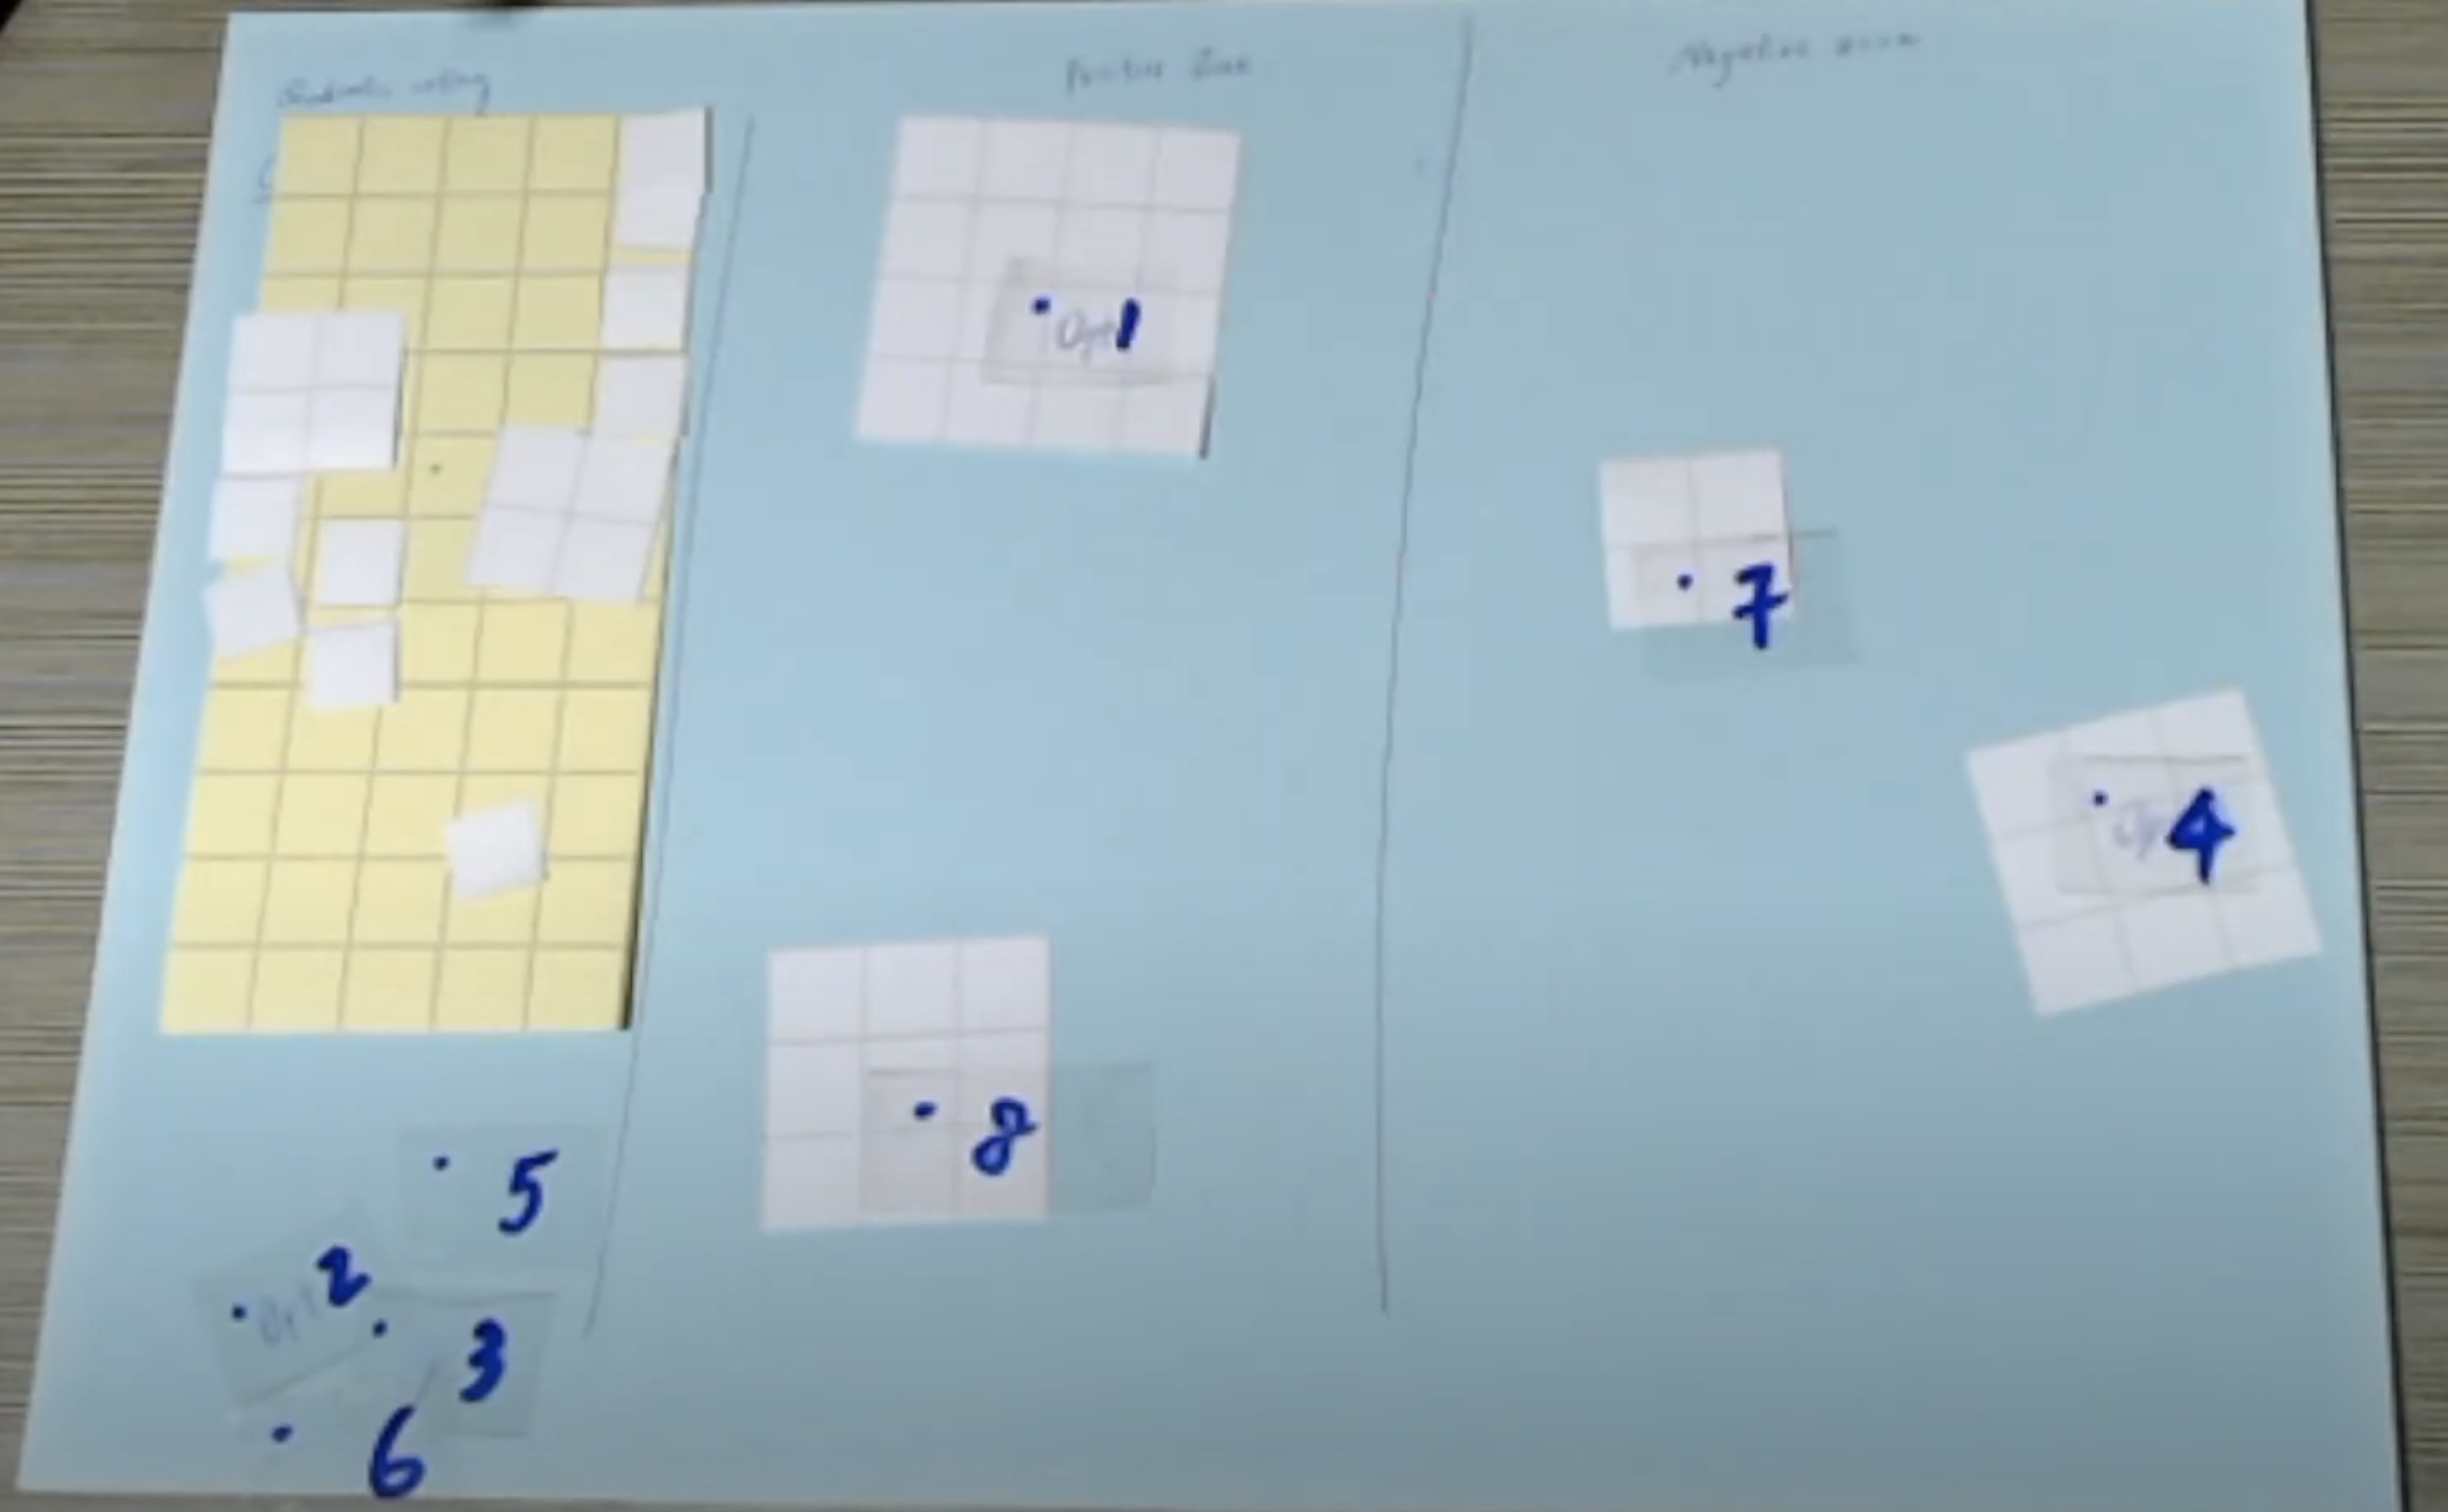
\includegraphics[width=\linewidth]{content/image/prototypes/1.2_paper_qv_single.png}
        \caption{In this paper prototype, issues are denoted by different numbers that appear on mouseover. Pretest respondents can move options anywhere in the two sections of the interface, one denoting positive and one negative. The blocks represent the cost for each option, with no indication of the number of current votes. The credits are shown in the yellow box on the left.}
        \Description{An image of a paper prototype showing different sections for respondents to interact with. On the left side, a yellow grid contains small white squares, some of which are stacked and scattered outside the grid. The middle section labeled "Positive Zone" contains a large white square with a grid, labeled "Opt 1". The right section, labeled "Negative Zone," contains two white squares, each with grids, labeled with numbers 7 and 4. Additional small white squares labeled with numbers 2, 3, 5, 6, and 8 are positioned around the prototype. The yellow box on the left represents available credits.}
        \label{fig:horizontal_paper}
    \end{subfigure}

    \vspace{1em} % Adjusts vertical spacing between figures

    % Second subfigure
    \begin{subfigure}[b]{0.9\linewidth}
        \centering
        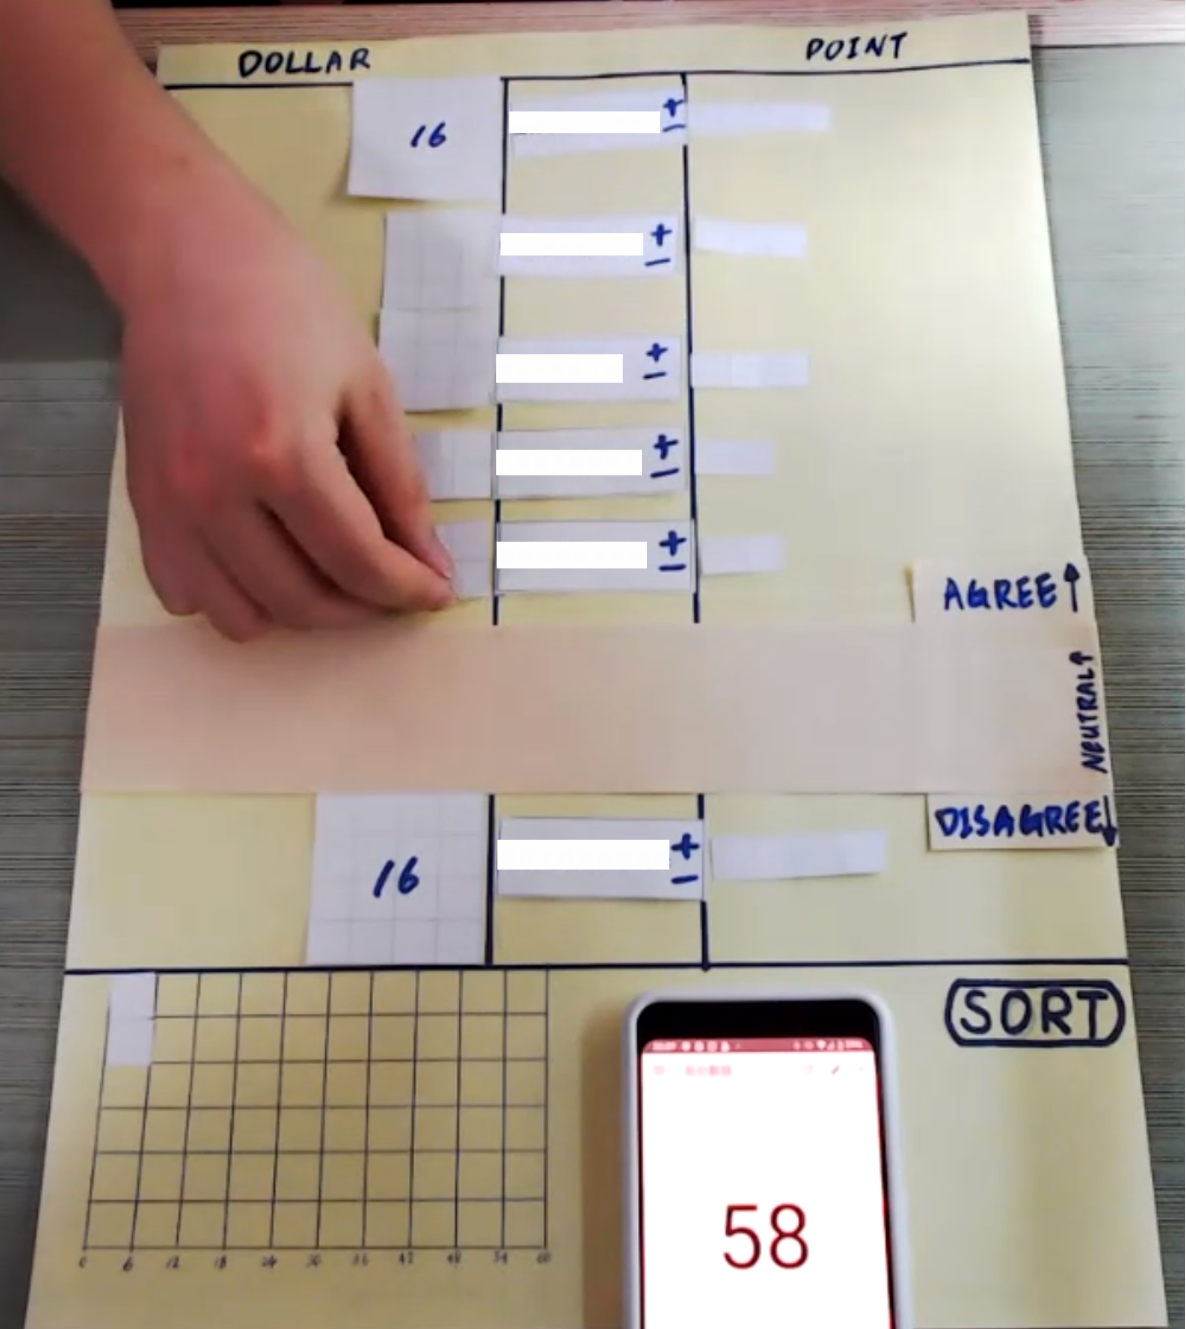
\includegraphics[width=\linewidth]{content/image/prototypes/1_paper_qv_single.png}
        \caption{This paper prototype separates the positive and negative areas with a 'band' at the center. Undecided options are placed inside this band. The cost and the votes on both sides of the interface are denoted by small blocks. The budget is shown in the yellow box below the interface with a numerical counter.}
        \Description{A paper prototype interface where a person's hand is interacting with blocks. The prototype separates positive and negative areas using a wide horizontal band in the center, which holds undecided options. On the left side of the band, a column labeled "Dollar" shows a block marked with the number 16. On the right side, under a column labeled "Point," several rows have small blocks with plus and minus signs, indicating positive and negative areas. At the bottom left, a yellow box with a grid shows the available budget, marked with the number 16. A smartphone in the bottom right corner displays the number 58.}
        \label{fig:vertical_paper}
    \end{subfigure}

    \caption{Initial paper prototypes designed for QS interface.}
    \Description{This figure contains two subfigures showing two different paper prototypes.}
    \label{fig:qv_paper}
\end{figure}


\subsection{Prototype 1: Ranking-Vote}
Considering that relative preference provides a ranked item, we tested whether ranking options before voting would help establish an individual's relative preference in Prototype 1. This prototype allowed respondents to reposition options before voting. Pretest respondents rarely moved the options and questioned the necessity of a full ranking, as it did not influence their QS submission. Additionally, many were unaware that options were draggable. This indicates that a full ranking is unnecessary for establishing relative preferences. Therefore, we decided to ask respondents to select a subset of options instead of requiring a full rank among all options.

\begin{figure}[ht]
    \centering
    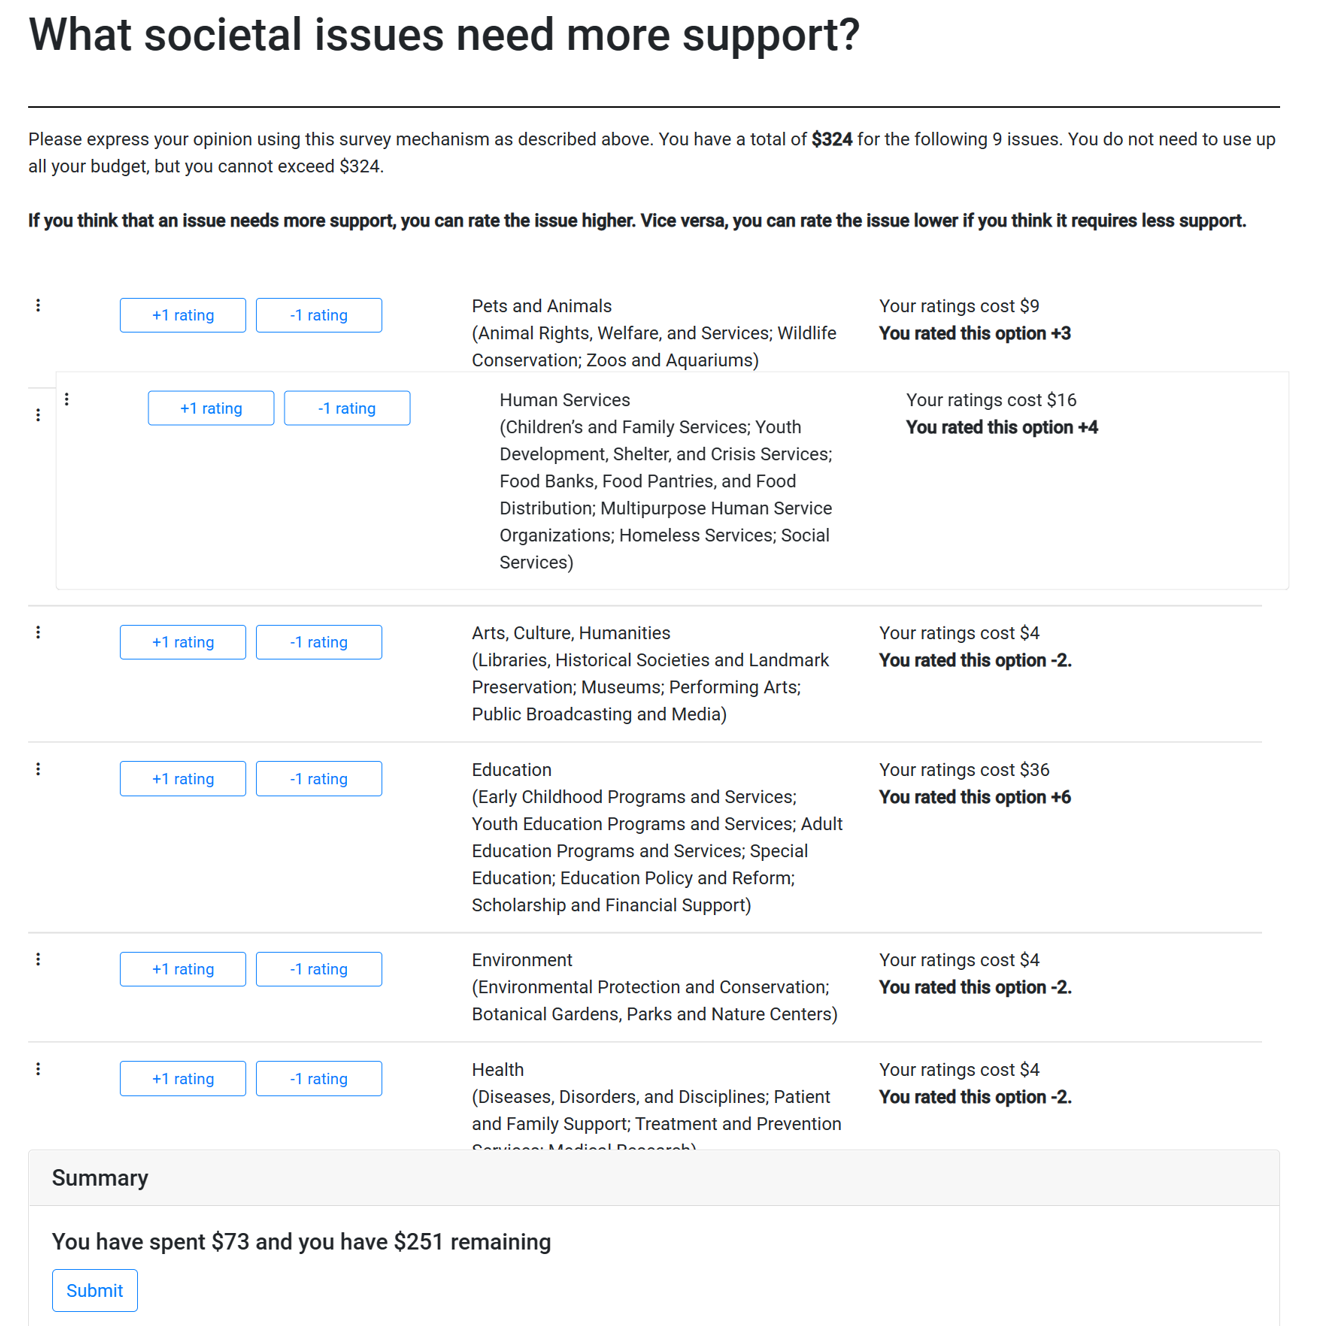
\includegraphics[width=0.43\textwidth]{content/image/prototypes/2_ranking.png}
    \caption{A Ranking-Vote Prototype: The goal of this prototype is to test whether ranking options prior to voting help establish an individual's relative preferences and reduce effort when voting. Each option is draggable to position in a specific location amongst the full list of options. Votes can be updated using the buttons to the right of the interface with vote count and costs to the right of the interface. A summary box is placed sticky to the bottom of the screen.}
    \Description{A web interface showing a survey titled "What societal issues need more support?" The interface presents several societal issues in a list format, each with buttons labeled "+1 rating" and "-1 rating" to adjust the ratings. For example, the issue "Pets and Animals" shows a rating cost of \$9 with a +3 rating, and "Human Services" shows a rating cost of \$16 with a +4 rating. The remaining issues include Arts, Culture, Humanities, Education, Environment, and Health, each with their respective ratings and costs. At the bottom of the page is a summary box displaying the total spent (\$73) and the remaining balance (\$251). A "Submit" button is positioned below the summary.}
    \label{fig:qv_rank}
    \vspace{-7ex}
\end{figure}

\begin{figure*}[p]
    \centering
    \begin{subfigure}[b]{0.47\textwidth}
        \centering
        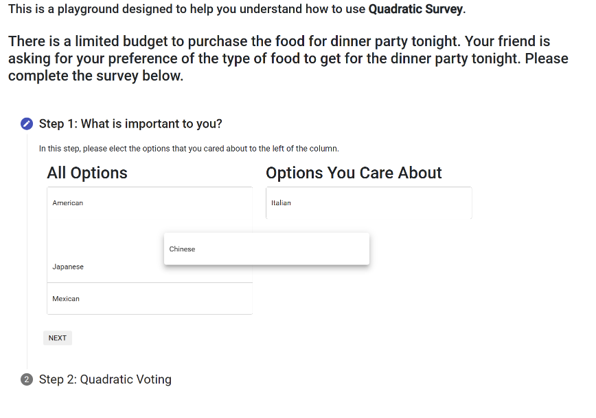
\includegraphics[width=0.95\textwidth]{content/image/prototypes/3.1_selecting.png}
        \caption{Options are dragged and dropped to the 'Option You Care About' box.}
        \Description{A web interface showing the first step of a quadratic voting prototype. The screen is titled "What is important to you?" On the left, under "All Options," a list of food types is displayed, including American, Japanese, and Mexican. One option, "Chinese," is being dragged to the right column labeled "Options You Care About," which already includes "Italian." A "Next" button appears at the bottom of the interface.}

        \label{fig:qv_select_selection}
    \end{subfigure}
    \hfill
    \begin{subfigure}[b]{0.47\textwidth}
        \centering
        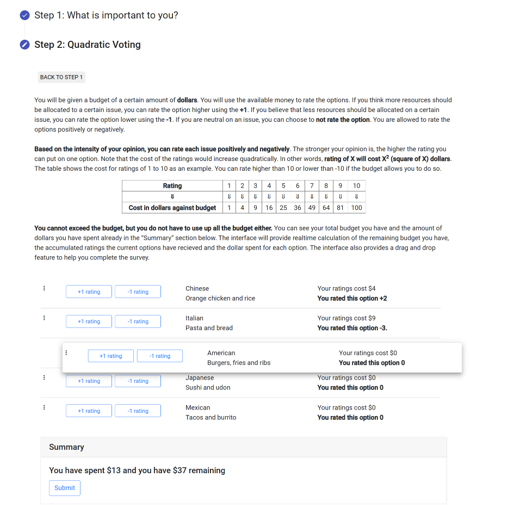
\includegraphics[width=0.9\textwidth]{content/image/prototypes/3.2_selecting_2.png}
        \caption{The previous step collapses showing all voting options.}
        \Description{The second step of a quadratic voting prototype showing a list of food options for voting. The voting interface displays food items such as Chinese, Pasta and bread, and American. Next to each item are "+1 rating" and "-1 rating" buttons for adjusting votes. Each option also shows the cost of votes, and a summary box at the bottom displays the amount spent (\$13) and the remaining balance (\$37).}

        \label{fig:qv_select_vote}
    \end{subfigure}
    \caption{A Select-then-Vote Prototype: The goal of this prototype is to nudge participants to focus on a subset of options to vote, rather than ranking all of them. This prototype introduces a two-step voting process. As shown in Fig.~\ref{fig:qv_select_selection}, the first step involves selecting options for further consideration. Important options are placed at the top of the list for voting shown in Fig.~\ref{fig:qv_select_vote}, but options can be placed anywhere on the list if desired. The rest of the controls follows the previous prototype.}
    \Description{A two-step quadratic voting prototype interface. In the first step (Subfigure 1), users drag and drop food options from a list on the left, such as American and Mexican, to the "Options You Care About" box on the right. In the second step (Subfigure 2), users vote on their selected options by adjusting the ratings using "+1 rating" and "-1 rating" buttons. A summary at the bottom shows the total amount spent and remaining balance.}

    \label{fig:qv_select}
\end{figure*}

\begin{figure*}[p]
    \centering
    \begin{subfigure}[b]{0.45\textwidth}
        \centering
        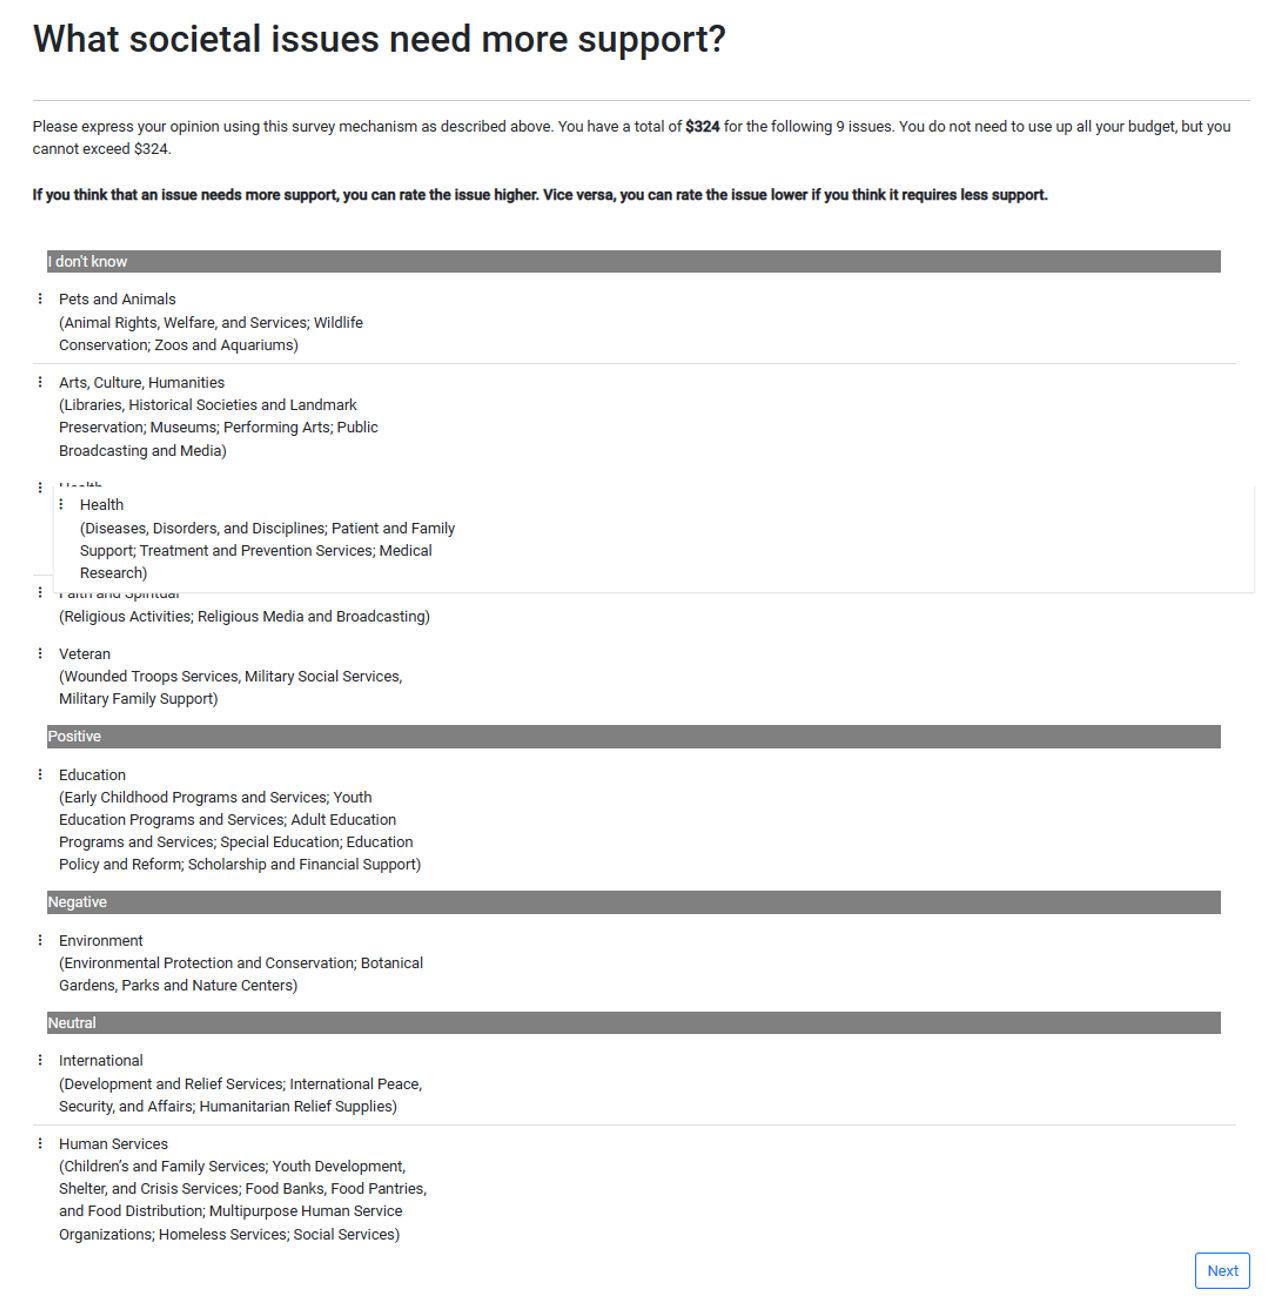
\includegraphics[width=\textwidth]{content/image/prototypes/4.1_grouping.png}
        \caption{The Organization Interface: Options are shown initially in the first bin labeled as `I don't know.' Survey respondents can then drag and drop these options into the latter bins: Lean Positive, Lean Neutral, or Lean Negative. Only the details of each option are shown on this interface.}
        \Description{A web interface displaying a survey titled "What societal issues need more support?" Initially, all options are placed in the first bin labeled "I don't know." The listed options include Pets and Animals, Arts, Culture, Humanities, Health, Veterans, and others. Each option is accompanied by a brief description. Below the "I don't know" bin are three other bins: "Positive," "Negative," and "Neutral." Survey respondents can drag and drop options into these bins based on their preferences. A "Next" button is located at the bottom right corner of the interface.}
        \label{fig:qv_org_p1}
    \end{subfigure}
    \hfill
    \begin{subfigure}[b]{0.45\textwidth}
        \centering
        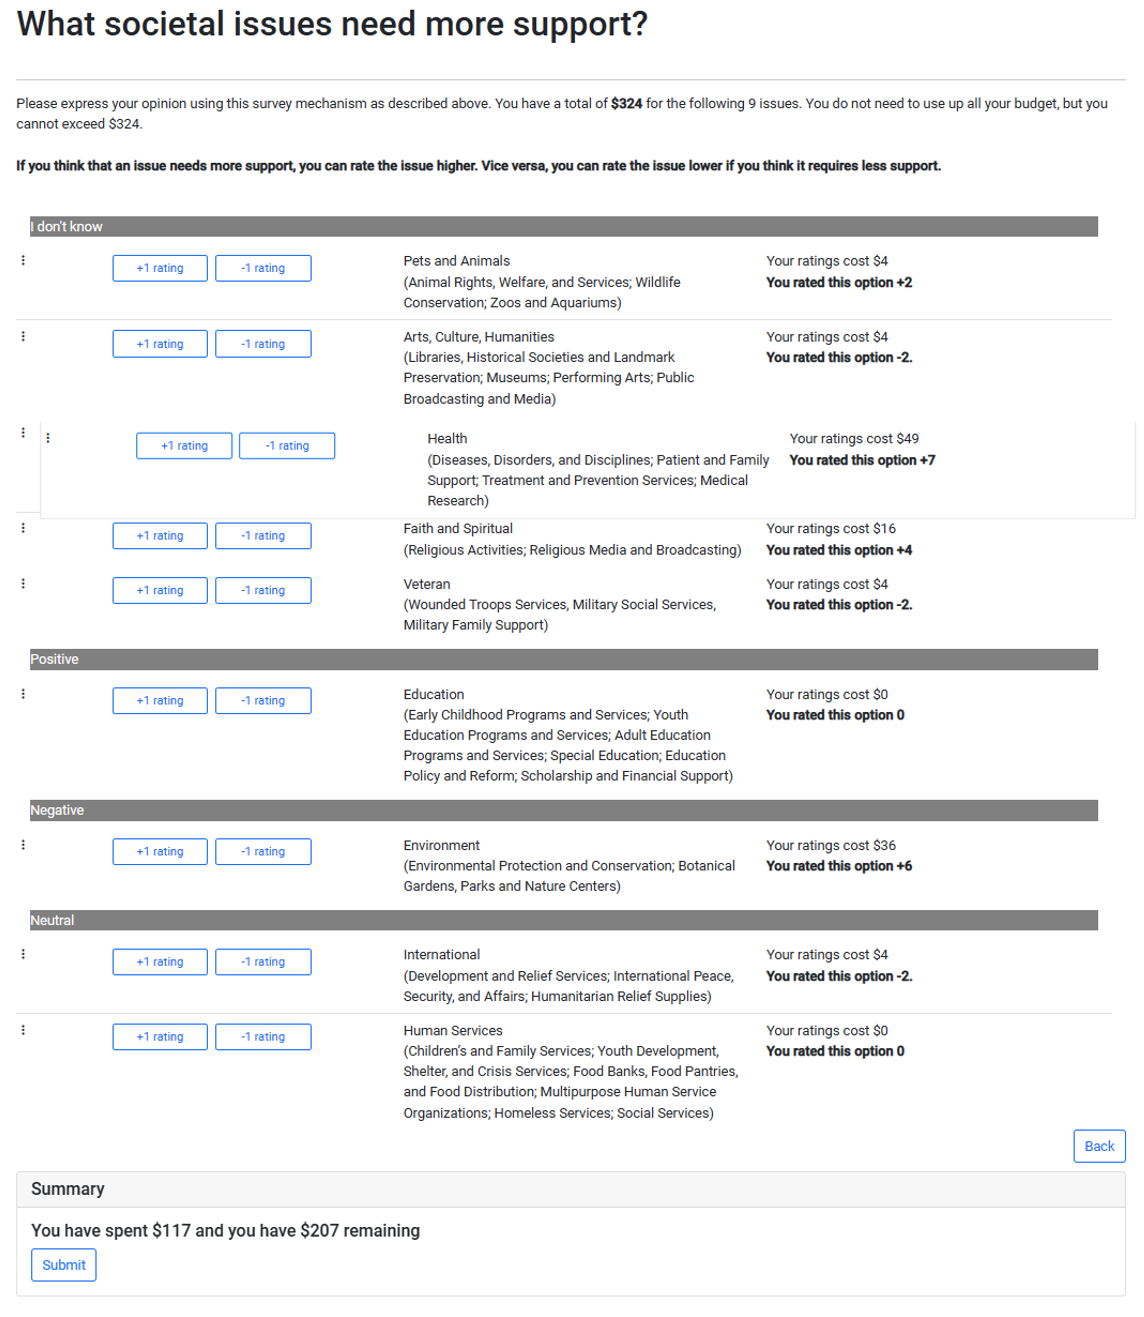
\includegraphics[width=\textwidth]{content/image/prototypes/4.2_grouping_vote.png}
        \caption{The Voting Interface: Voting controls appear on the left side of each option, showing the current votes and associated costs on the right. A budget summary sticks to the bottom of the screen.}
        \Description{A web interface displaying a survey titled "What societal issues need more support?" Each option in the list has voting controls, with "+1 rating" and "-1 rating" buttons appearing on the left side of each issue. The issues are grouped into categories such as "I don't know," "Positive," "Negative," and "Neutral." To the right of each issue, the cost of the rating is shown along with the number of votes cast. For example, "Pets and Animals" has a rating cost of \$4 with a +2 rating, while "Health" has a rating cost of \$49 with a +7 rating. At the bottom of the page, a summary box shows the total amount spent (\$117) and the remaining balance (\$207), with a "Submit" button below it.}

        \label{fig:qv_org_p2}
    \end{subfigure}
    \caption{Organize-then-Vote Prototype: The goal of this prototype is to encourage participants to derive finer grain categories among options before voting. Survey respondents first organize their thoughts into categories and then vote on the options.}
    \Description{The figure shows an Organize-then-Vote prototype with two main steps. In the first step, the left figure, users organize options by dragging and dropping them into different categories: "I don't know," "Positive," "Neutral," or "Negative." In the second step, the right figure, users vote on these organized options using "+1 rating" and "-1 rating" buttons, with voting costs and current ratings displayed. A summary section shows the total spent and remaining budget.}
    \label{fig:qv_org}
\end{figure*}

\subsection{Prototype 2: Select-then-Vote}
Based on feedback from Prototype 1, instead of \textit{allowing} individuals to rank options, Prototype 2 implemented a two-phase process that \textit{intentionally} asks respondents to select options to express opinions before voting. As shown in Figure~\ref{fig:qv_select}, survey respondents selected their preferred options (Figure~\ref{fig:qv_select_selection}), and the interface positioned these options at the top of the list for voting (Figure~\ref{fig:qv_select_vote}). We identified several issues during the prototype 2 pretest: many respondents marked most options as 'options they care about,' which undermined the design's purpose. Additionally, the lack of clear distinction between selected and unselected options confused respondents about the necessity of Step 1. Thus, we need a clearer distinction and connection between the two phases to effectively construct relative preferences.

\subsection{Prototype 3: Organize-then-Vote}
Figure~\ref{fig:qv_org} shows the last prototype where we built on the previous takeaway by providing finer-grain groupings and creating a clear connection between option organization and voting position. Specifically, we provided three categories: Lean Positive, Lean Negative, and Lean Neutral. Initially, respondents see all options under the section labeled 'I don't know,' which includes only the option descriptions. We ask respondents to move these options into the categories below. Voting controls and information appear on each option once respondents move to the subsequent page, forming a clear connection between option groups, positions, and voting controls.

Feedback indicated that survey respondents are comfortable with the two-phase organize-then-vote design, demonstrating it as a central strategy for our interface development. However, several areas for enhancement were identified: First, the dragging and dropping mechanism in the organization phase is cumbersome and may inadvertently suggest a ranking process, contrary to our intentions. Second, placing unorganized options at the top of the voting list is counterintuitive. Third, the voting controls are disconnected from the option summaries, dividing attention between the left and right sides of the screen. These insights guided refinements in the final two-phase interface, adhering to the two-phase organize-then-vote design framework.

% \section{Voting Interface Breakdown}\label{apdx:relatedVoting}
In this section, we outline additional literature that informed this study. There are two sets of literature that we surveyed: Survey response format and voting interfaces.

\subsection{Survey response format}
Research in the marketing and research communities focusing on survey and questionnaire design, usability, and interactions examines the influence of presentation styles and `response format.'~\citet{weijtersExtremityHorizontalVertical2021} demonstrated that horizontal distances between options are more influential than vertical distances, with the latter recommended for reduced bias. Slider bars, which operate on a drag-and-drop principle, show lower mean scores and higher nonresponse rates compared to buttons, indicating they are more prone to bias and difficult to use. In contrast, visual analog scales that operate on a point-and-click principle perform better~\cite{toepoelSlidersVisualAnalogue2018}. These studies show how even small design changes can have a large impact on usability, highlighting the importance of designing interfaces that prioritize human-centered interaction rather than focusing solely on functionality.

\subsection{Voting Interfaces}
Compared to digital survey interfaces, voting interfaces are a specialized type of survey interface can significantly influence democratic processes~\cite{engstrom2020politics, chisnellDemocracyDesignProblem2016, civicdesignDesigningUsableBallots2015} and often have consequential impacts. Researchers believe that ill-designed voting interfaces We categorize these related works into three main categories detailed below:

\paragraph{Designs that shifted voter decisions: } For example, states without straight-party ticket voting~(where voters can select all candidates from one party through a single choice) exhibited higher rates of split-ticket voting~\cite{engstrom2020politics}. Another example from the Australian ballot showing incumbency advantages is where candidates are listed by the office they are running for, with no party labels or boxes.

\paragraph{Designs that influenced errors: } Butterfly ballots, an atypical design, may have influenced the outcome of the 2000 U.S. Presidential Election~\cite{wandButterflyDidIt2001}. It increased voter errors because voters could not correctly identify the punch hole on the ballot. Splitting contestants across columns increases the chance for voters to overvote~\cite{quesenberyOpinionGoodDesign2020}. On the other hand, \citet{everettElectronicVotingMachines2008} showed the use of incorporating physical voting behaviors, like lever voting, into graphical user interfaces.

\paragraph{Designs that incorporated technologies: } Other projects like the Caltech-MIT Voting Technology Project have sparked research to address accessibility challenges, resulting in innovations like EZ Ballot~\cite{leeUniversalDesignBallot2016}, Anywhere Ballot~\cite{summers2014making}, and Prime III~\cite{dawkinsPrimeIIIInnovative2009}. In addition,~\citet{gilbertAnomalyDetectionElectronic2013} investigated optimal touchpoints on voting interfaces, and~\citet{conradElectronicVotingEliminates2009} examined zoomable voting interfaces.

Response format literature and voting interfaces informed how interfaces significantly influence respondent behavior, decision accuracy, and cognitive load. These burdens are especially problematic for complex systems like QS, where high cognitive demands may deter researchers and users alike. Developing effective, human-centered interfaces for QS could enhance usability, reduce cognitive overload, and increase adoption in both research and practical applications.

% \begin{figure}
    \centering
    \begin{subfigure}[h]{0.6\textwidth}
        \centering
        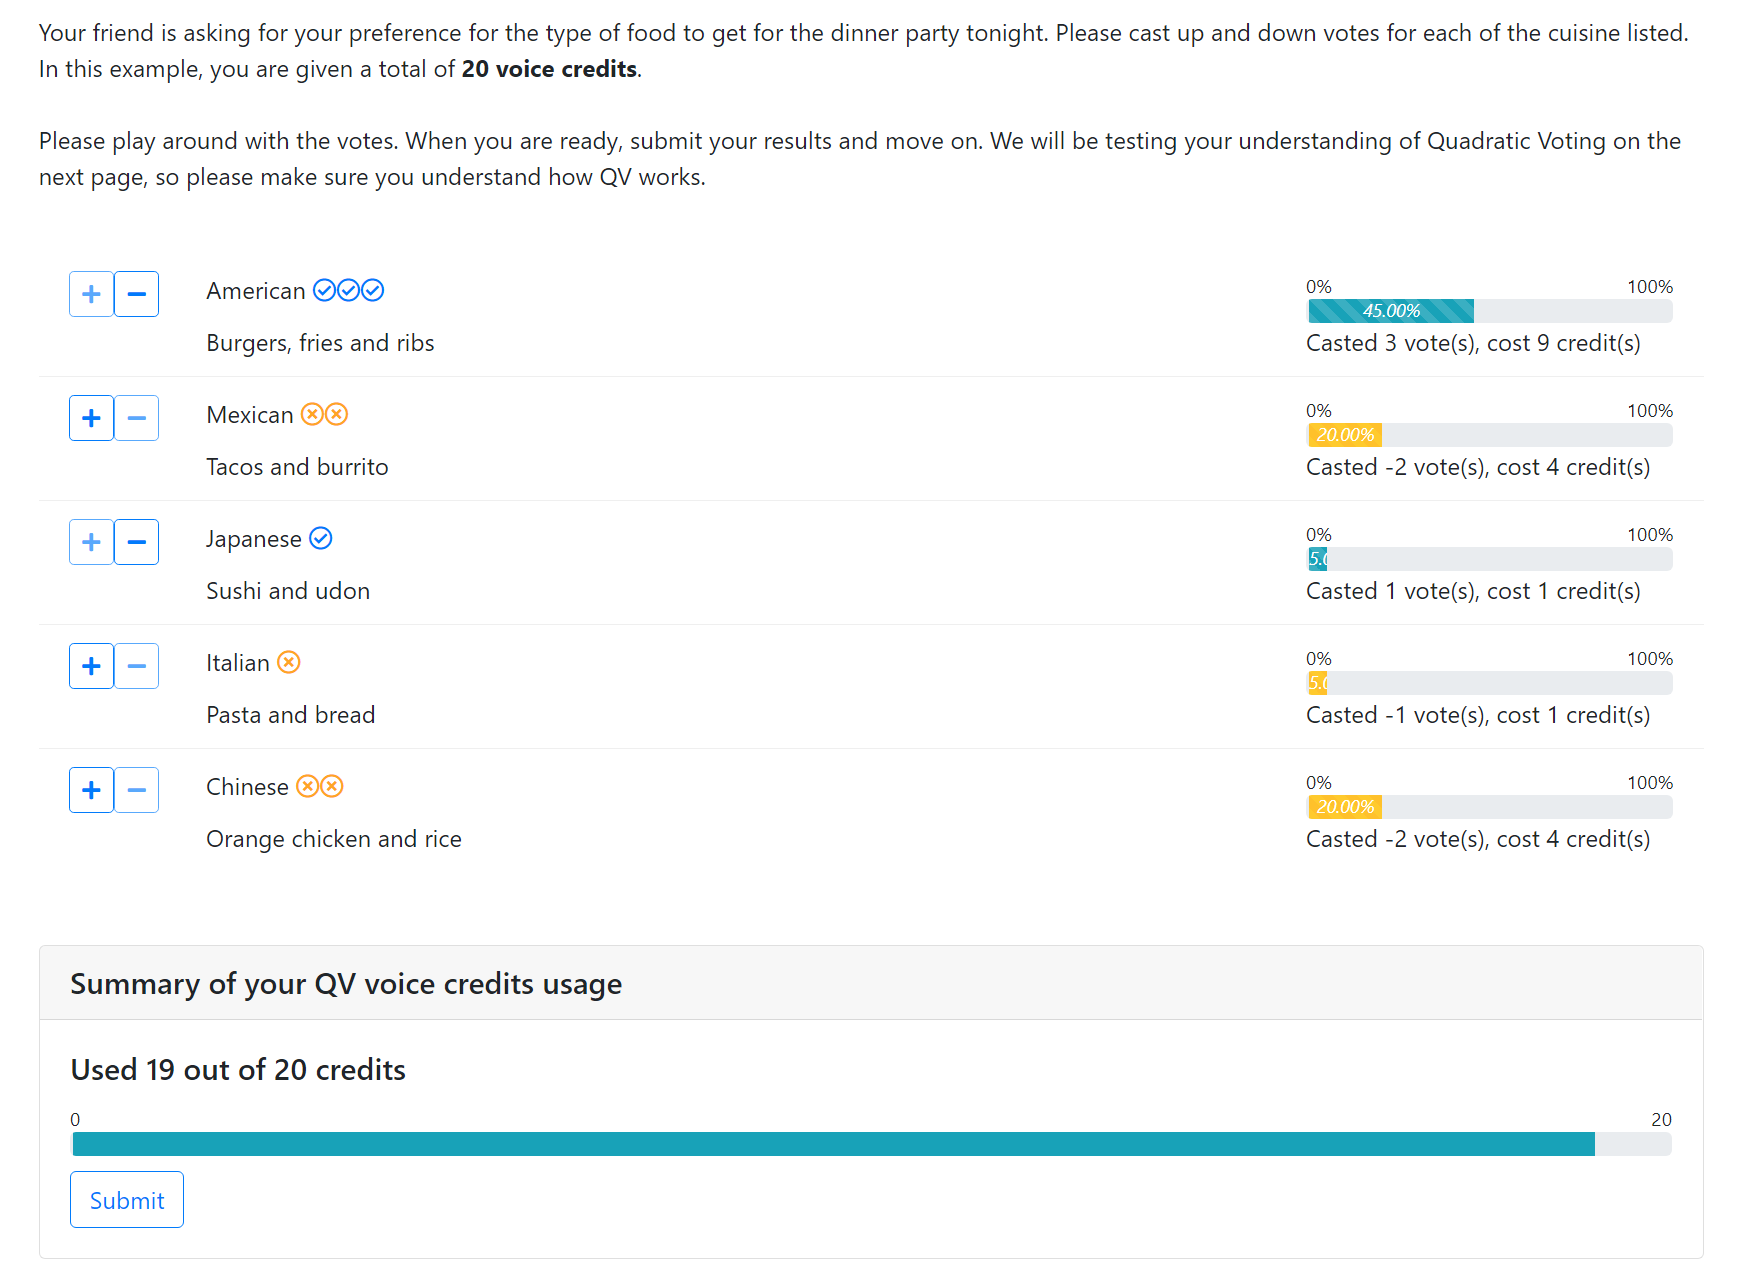
\includegraphics[width=\textwidth]{content/image/curr_interface/cheng_qv.png}
        \caption{The interface used in the research by~\textcite{chengCanShowWhat2021}.}
        \label{fig:chengInterface}
    \end{subfigure}
    \caption{Recent implementations of interfaces applying the quadratic mechanism (1/2).}
    \label{fig:recentInterfaces1}
\end{figure}

\begin{figure}
    \ContinuedFloat
    \centering
    \begin{subfigure}[h]{0.6\textwidth}
        \centering
        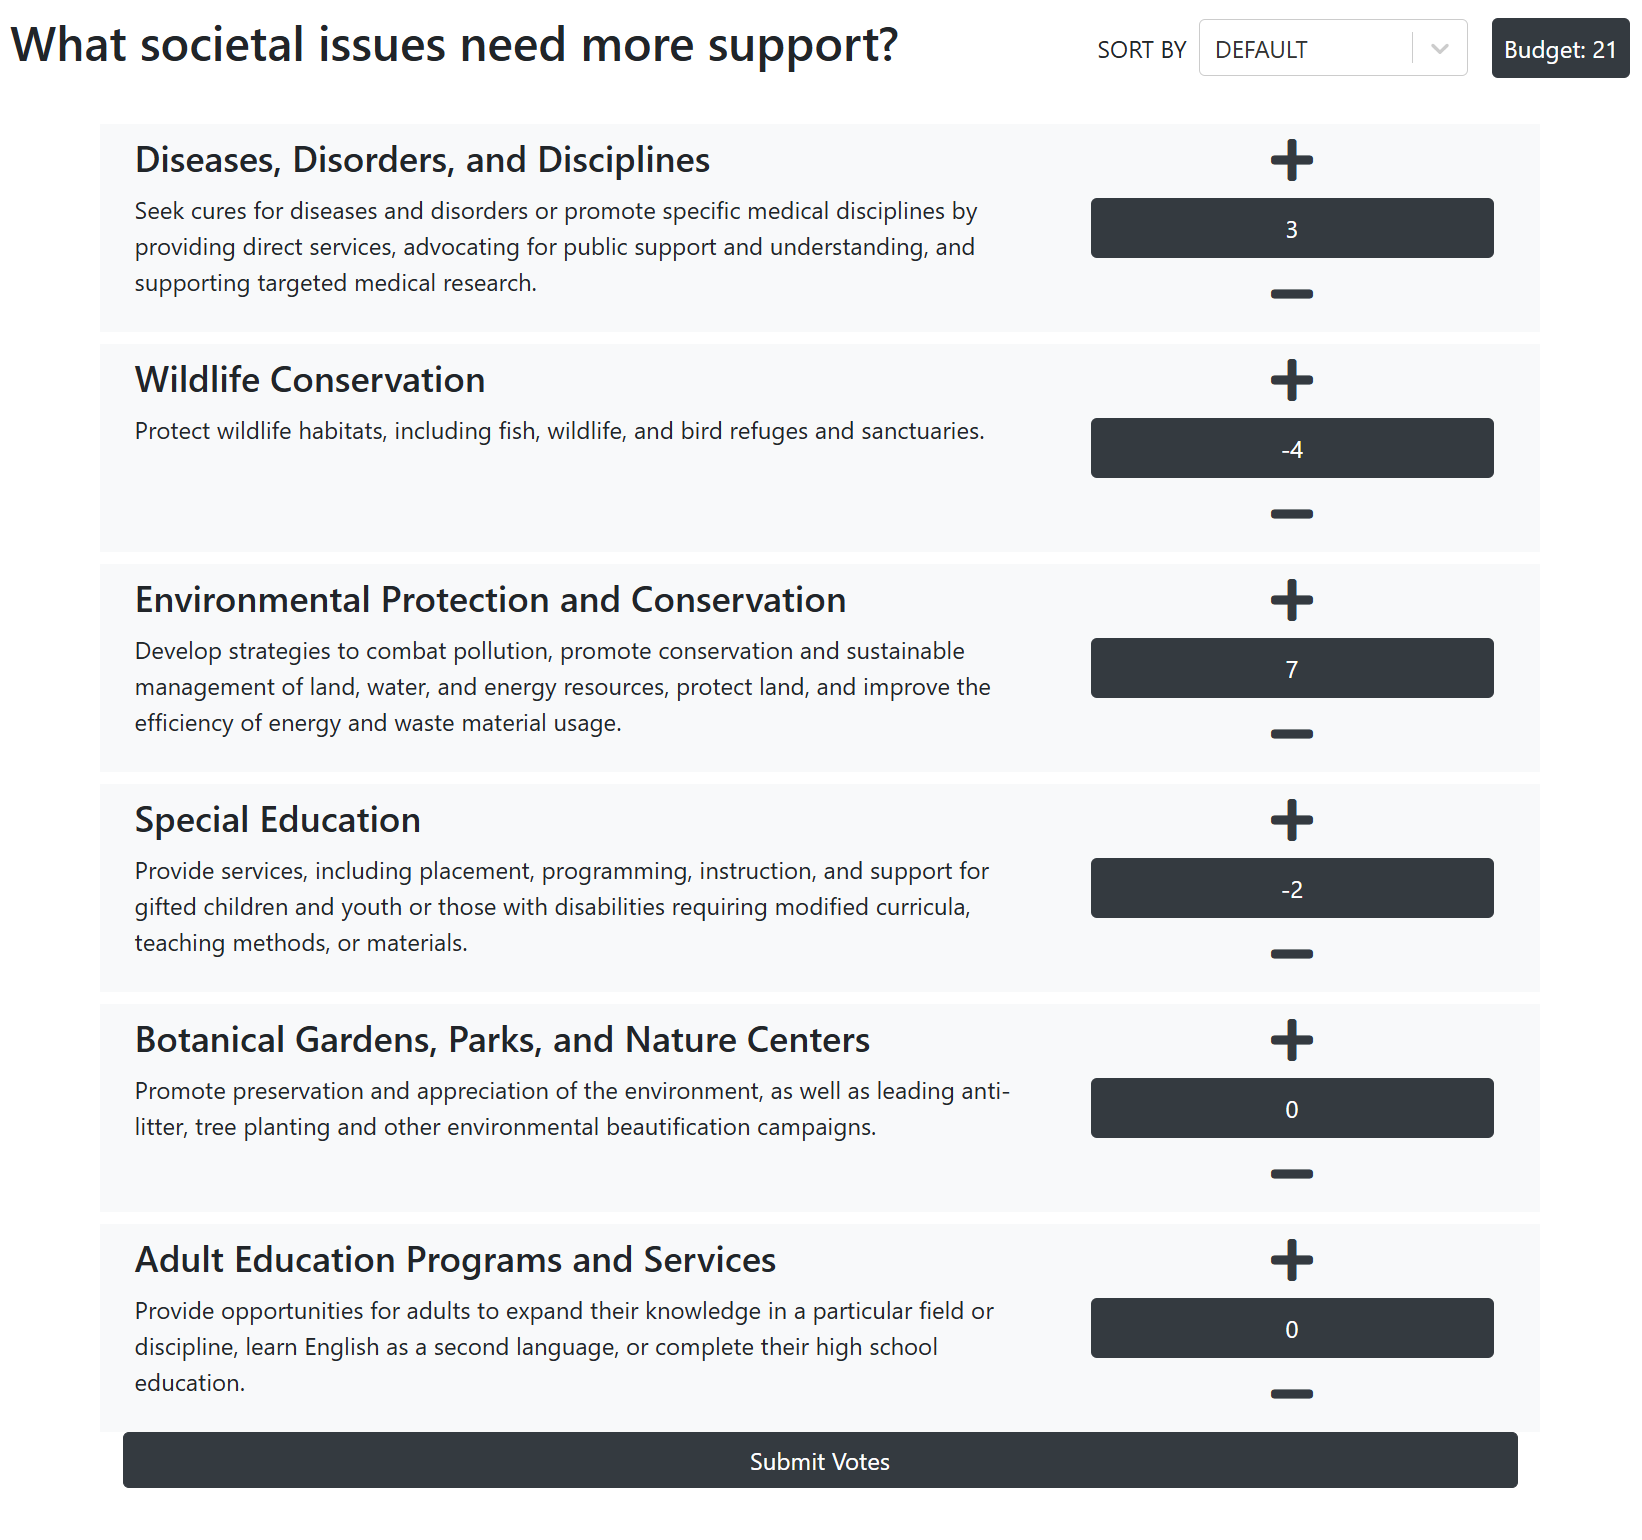
\includegraphics[width=\textwidth]{content/image/curr_interface/geek.sg_interface.png}
        \caption{An open-source QV interface~\cite{yehjxraymondYehjxraymondQvapp2024} that offers a publicly available service.}
        \label{fig:fig2}
    \end{subfigure}
    \begin{subfigure}[h]{0.6\textwidth}
        \centering
        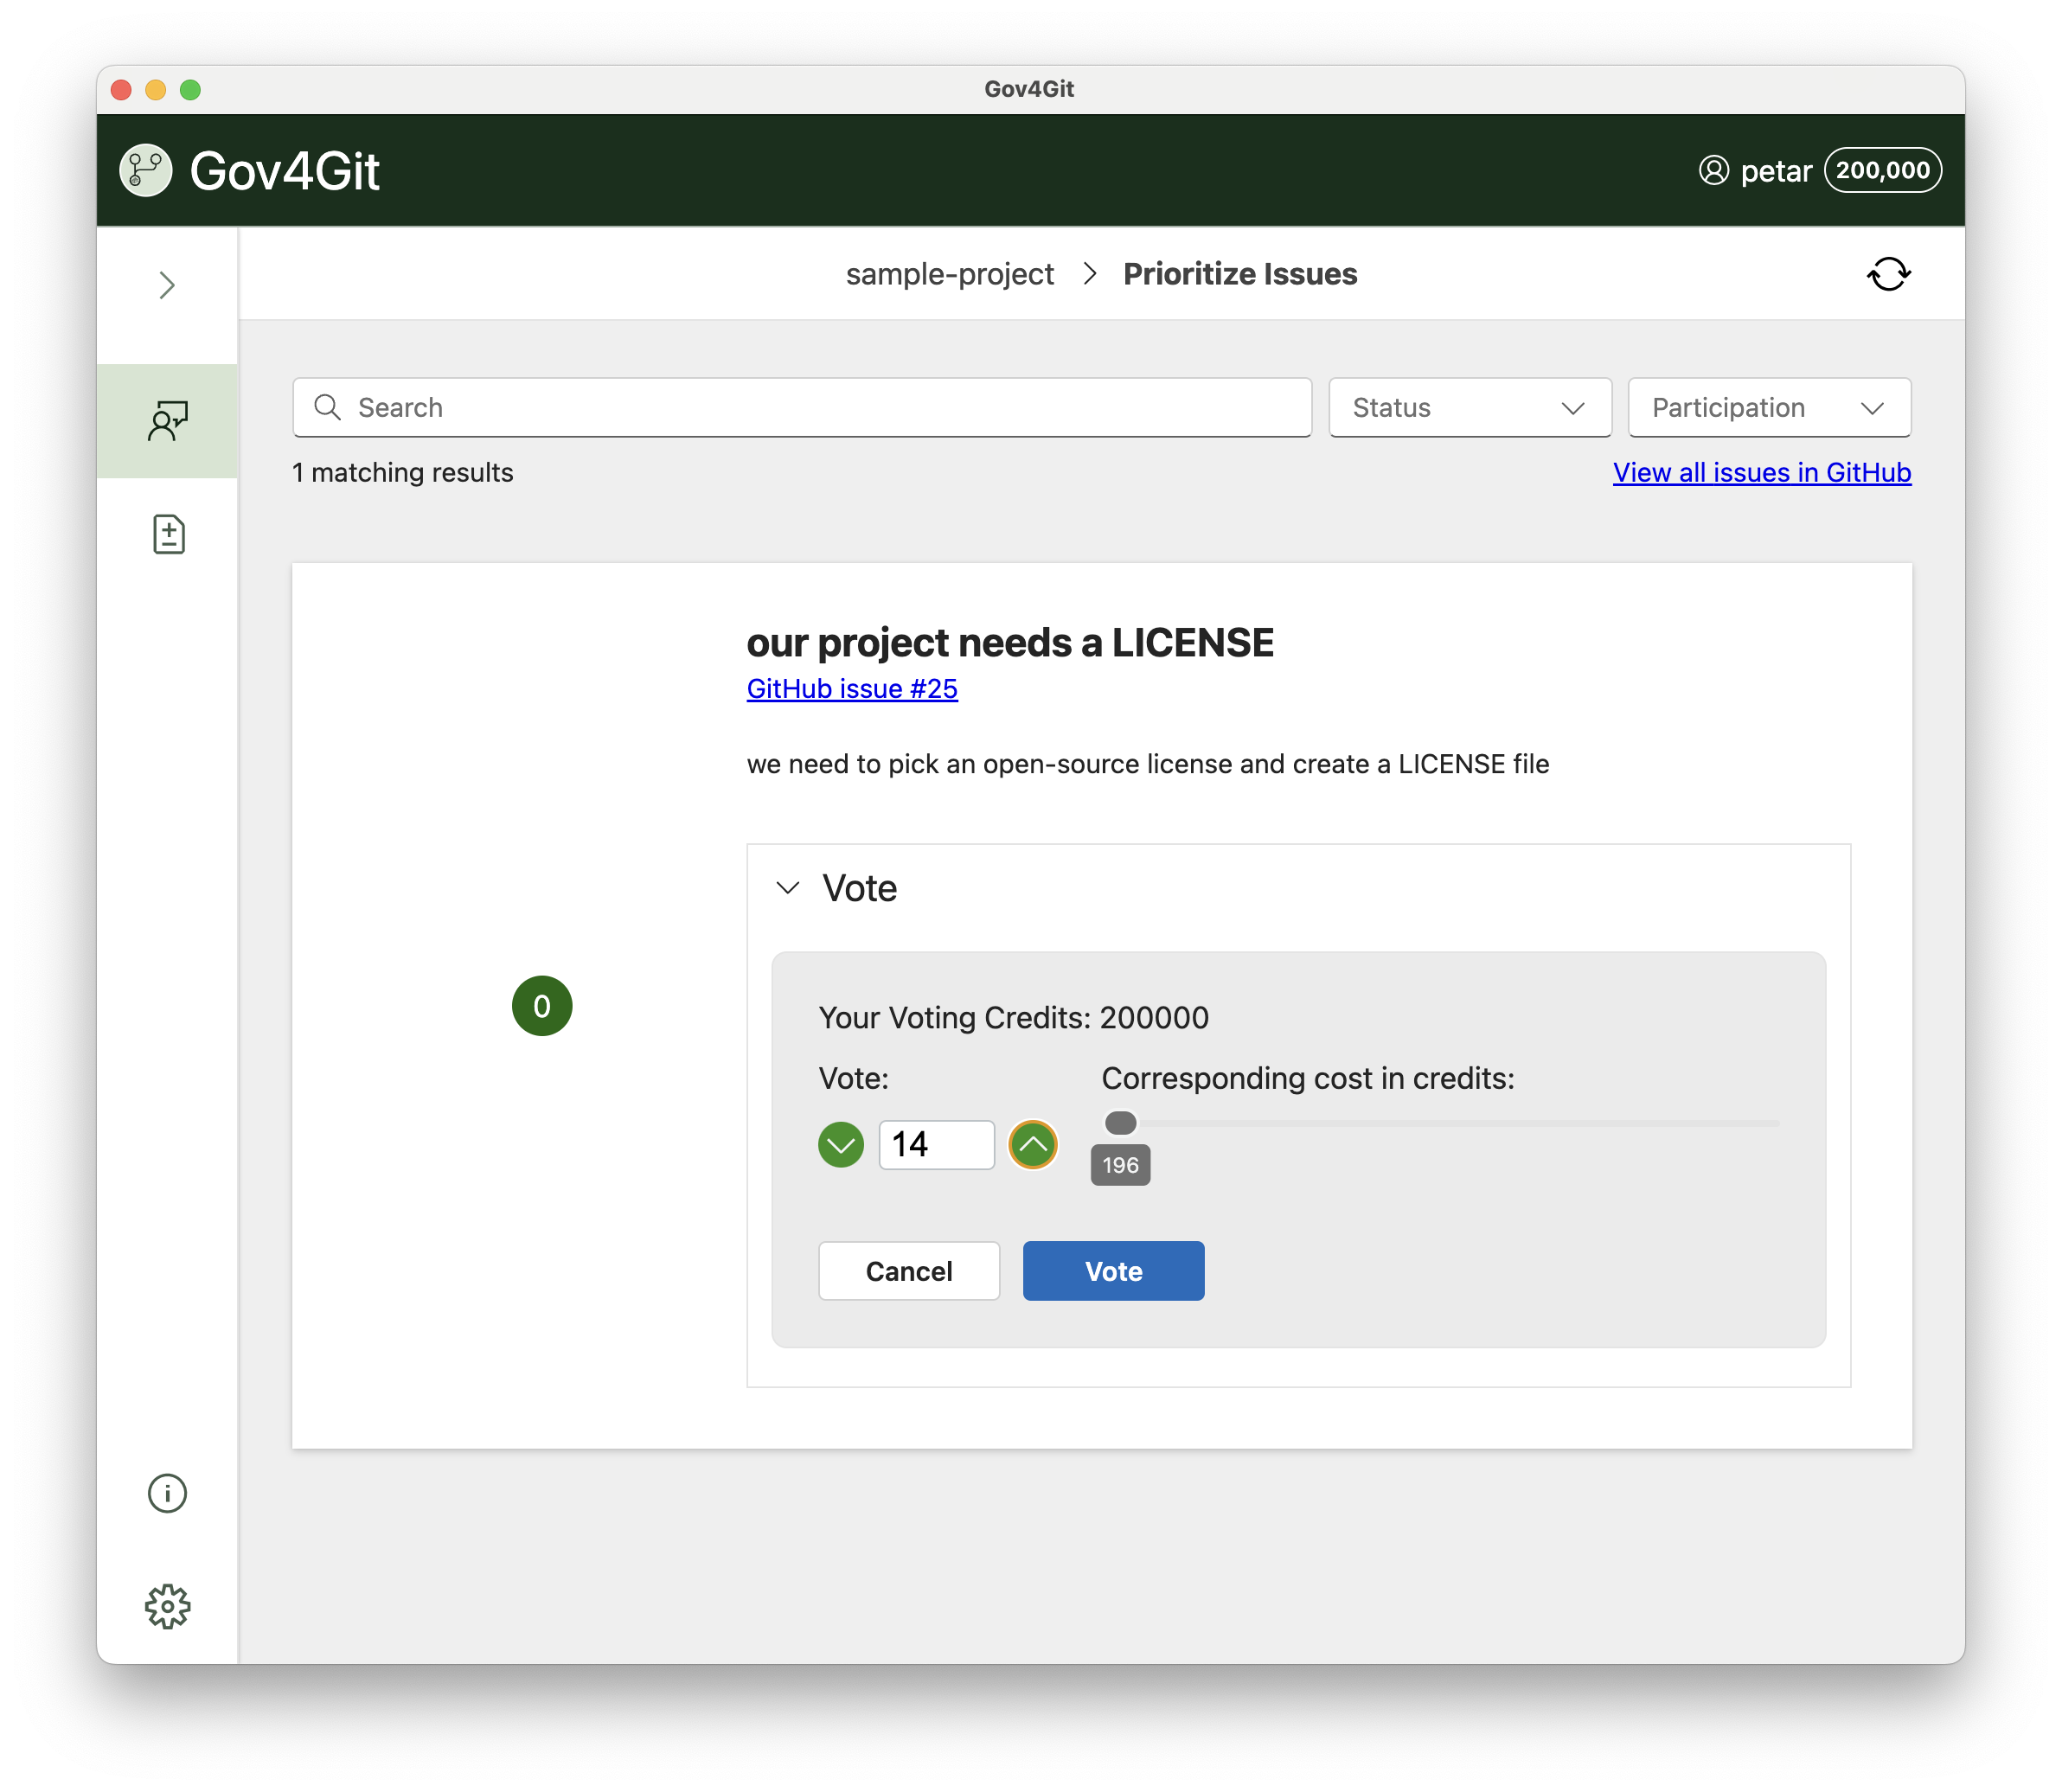
\includegraphics[width=\textwidth]{content/image/curr_interface/appvote.png}
        \caption{The interface designed for gov4git~\cite{Gov4gitDecentralizedPlatform2023}.}
        \label{fig:fig3}
    \end{subfigure}
    \caption{Recent implementations of interfaces applying the quadratic mechanism (2/2).}
    \label{fig:recentInterfaces2}
\end{figure}

% \newpage

% % Experimental Setup Appendix
% \section{Experimental Setup}
% \section{Demographic Breakdown}
\label{sec:apdx:demo}
We provide the table for a more detail demographic breakdown per group.
\begin{table}[h!]
\centering
\caption{Participant Age and Gender Distribution by Experimental Condition}
\label{tab:age_gender_distribution}
\begin{tabular}{lcccccccccc}
\hline
\textbf{Condition} & \textbf{Mean Age} & \textbf{SD} & \textbf{Range} & \textbf{25th} & \textbf{Median} & \textbf{75th} & \textbf{Male} & \textbf{Female} & \textbf{Non-binary} \\
\hline
Short Text      & 31.6  & 13.7 & 18--67 & 23.8 & 29.5 & 32.8 & 4 & 6 & 0 \\
Short 2 Phase   & 32.1  & 14.0 & 18--52 & 20.3 & 27.0 & 44.5 & 4 & 6 & 0 \\
Long Text       & 36.0  & 14.8 & 21--61 & 24.0 & 33.0 & 42.8 & 2 & 7 & 1 \\
Long 2 Phase    & 38.8  & 19.6 & 19--71 & 25.0 & 28.5 & 53.0 & 2 & 8 & 0 \\
\hline
\end{tabular}
\Description{ A table summarizing participant demographics and descriptive statistics for four conditions: Short Text, Short 2-Phase, Long Text, and Long 2-Phase.}
\end{table}

% \section{List of Options}
\label{sec:charityList}
We provide the full list of options presented on the survey.

\begin{itemize}[leftmargin=*]
    \item \textbf{Animal Rights, Welfare, and Services:} Protect animals from cruelty, exploitation and other abuses, provide veterinary services and train guide dogs.
    \item \textbf{Wildlife Conservation:} Protect wildlife habitats, including fish, wildlife, and bird refuges and sanctuaries.
    \item \textbf{Zoos and Aquariums:} Support and invest in zoos, aquariums and zoological societies in communities throughout the country.
    \item \textbf{Libraries, Historical Societies and Landmark Preservation:} Support and invest public and specialized libraries, historical societies, historical preservation programs, and historical estates.
    \item \textbf{Museums:} Support and invest in maintaining collections and provide training to practitioners in traditional arts, science, technology, and natural history.
    \item \textbf{Performing Arts:} Support symphonies, orchestras, and other musical groups; ballets and operas; theater groups; arts festivals; and performance halls and cultural centers.
    \item \textbf{Public Broadcasting and Media:} Support public television and radio stations and networks, as well as providing other independent media and communications services to the public.
    \item \textbf{Community Foundations:} Promote giving by managing long-term donor-advised charitable funds for individual givers and distributing those funds to community-based charities over time.
    \item \textbf{Housing and Neighborhood Development:} Lead and finance development projects that invest in and improve communities by providing utility assistance, small business support programs, and other revitalization projects.
    \item \textbf{Jewish Federations:} Focus on a specific geographic region and primarily support Jewish-oriented programs, organizations and activities through grantmaking efforts
    \item \textbf{United Ways:} Identify and resolve community issues through partnerships with schools, government agencies, businesses, and others, with a focus on education, income and health.
    \item \textbf{Adult Education Programs and Services:} Provide opportunities for adults to expand their knowledge in a particular field or discipline, learn English as a second language, or complete their high school education.
    \item \textbf{Early Childhood Programs and Services:} Provide foundation-level learning and literacy for children prior to entering the formal school setting.
    \item \textbf{Education Policy and Reform:} Promote and provide research, policy, and reform of the management of educational institutions, educational systems, and education policy.
    \item \textbf{Scholarship and Financial Support:} Support and enable students to obtain the financial assistance they require to meet their educational and living expenses while in school.
    \item \textbf{Special Education:} Provide services, including placement, programming, instruction, and support for gifted children and youth or those with disabilities requiring modified curricula, teaching methods, or materials.
    \item \textbf{Youth Education Programs and Services:} Provide programming, classroom instruction, and support for school-aged students in various disciplines such as art education, STEM, outward bound learning experiences, and other programs that enhance formal education.
    \item \textbf{Botanical Gardens, Parks, and Nature Centers:} Promote preservation and appreciation of the environment, as well as leading anti-litter, tree planting and other environmental beautification campaigns.
    \item \textbf{Environmental Protection and Conservation:} Develop strategies to combat pollution, promote conservation and sustainable management of land, water, and energy resources, protect land, and improve the efficiency of energy and waste material usage.
    \item \textbf{Diseases, Disorders, and Disciplines:} Seek cures for diseases and disorders or promote specific medical disciplines by providing direct services, advocating for public support and understanding, and supporting targeted medical research.
    \item \textbf{Medical Research:} Devote and invest in efforts on researching causes and cures of disease and developing new treatments.
    \item \textbf{Patient and Family Support:} Support programs and services for family members and patients that are diagnosed with a serious illness, including wish granting programs, camping programs, housing or travel assistance.
    \item \textbf{Treatment and Prevention Services:} Provide direct medical services and educate the public on ways to prevent diseases and reduce health risks.
    \item \textbf{Advocacy and Education:} Support social justice through legal advocacy, social action, and supporting laws and measures that promote reform and protect civil rights, including election reform and tolerance among diverse groups.
    \item \textbf{Development and Relief Services:} Provide medical care and other human services as well as economic, educational, and agricultural development services to people around the world.
    \item \textbf{Humanitarian Relief Supplies:} Specialize in collecting donated medical, food, agriculture, and other supplies and distributing them overseas to those in need.
    \item \textbf{International Peace, Security, and Affairs:} Promote peace and security, cultural and student exchange programs, improve relations between particular countries, provide foreign policy research and advocacy, and United Nations-related organizations.
    \item \textbf{Religious Activities:} Support and promote various faiths.
    \item \textbf{Religious Media and Broadcasting:} Support organizations of all faiths that produce and distribute religious programming, literature, and other communications.
    \item \textbf{Non-Medical Science \& Technology Research:} Support research and services in a variety of scientific disciplines, advancing knowledge and understanding of areas such as energy efficiency, environmental and trade policies, and agricultural sustainability.
    \item \textbf{Social and Public Policy Research:} Support economic and social issues impacting our country today, educate the public, and influence policy regarding healthcare, employment rights, taxation, and other civic ventures.
\end{itemize}


% \begin{table}[h!]
% \centering
% \caption{Full List of Survey Options}
% \label{tab:optionsList}
% \begin{tabular}{p{3.4cm} p{12cm}}
% \toprule
% \textbf{Category} & \textbf{Description} \\
% \midrule
% Animal Rights, Welfare, and Services & Protect animals from cruelty, exploitation, and other abuses, provide veterinary services, and train guide dogs. \\
% Wildlife Conservation & Protect wildlife habitats, including fish, wildlife, and bird refuges and sanctuaries. \\
% Zoos and Aquariums & Support and invest in zoos, aquariums, and zoological societies in communities throughout the country. \\
% Libraries, Historical Societies, and Landmark Preservation & Support public and specialized libraries, historical societies, preservation programs, and historical estates. \\
% Museums & Support and invest in maintaining collections and providing training to practitioners in traditional arts, science, technology, and natural history. \\
% Performing Arts & Support symphonies, orchestras, ballets, operas, theater groups, arts festivals, and cultural centers. \\
% Public Broadcasting and Media & Support public television and radio stations and networks, as well as independent media and communications services. \\
% Community Foundations & Promote giving by managing donor-advised charitable funds and distributing them to community-based charities over time. \\
% Housing and Neighborhood Development & Lead and finance projects to improve communities by providing utility assistance, small business support, and revitalization projects. \\
% Jewish Federations & Support Jewish-oriented programs, organizations, and activities through grantmaking efforts. \\
% United Ways & Identify and resolve community issues through partnerships with schools, government agencies, businesses, and others. \\
% Adult Education Programs and Services & Provide opportunities for adults to expand their knowledge, learn English as a second language, or complete their high school education. \\
% Early Childhood Programs and Services & Provide foundation-level learning and literacy for children before formal schooling. \\
% Education Policy and Reform & Promote research, policy, and reform of educational institutions and systems. \\
% Scholarship and Financial Support & Support students to obtain financial assistance for educational and living expenses. \\
% Special Education & Provide services for gifted children and youth or those with disabilities requiring modified curricula or teaching methods. \\
% Youth Education Programs and Services & Provide programming for school-aged students in disciplines such as art, STEM, and outward-bound learning. \\
% Botanical Gardens, Parks, and Nature Centers & Promote preservation of the environment and lead environmental beautification campaigns. \\
% Environmental Protection and Conservation & Develop strategies to combat pollution, promote conservation, and manage resources sustainably. \\
% Diseases, Disorders, and Disciplines & Seek cures for diseases and disorders and promote specific medical disciplines. \\
% Medical Research & Research causes and cures of diseases and develop new treatments. \\
% Patient and Family Support & Support programs for family members and patients diagnosed with serious illnesses. \\
% Treatment and Prevention Services & Provide medical services and educate the public on disease prevention and health risks. \\
% Advocacy and Education & Support social justice through legal advocacy, social action, and reform measures. \\
% Development and Relief Services & Provide medical care, human services, and economic, educational, and agricultural development services. \\
% Humanitarian Relief Supplies & Distribute donated medical, food, agricultural, and other supplies to those in need. \\
% International Peace, Security, and Affairs & Promote peace, security, cultural exchanges, and improve international relations. \\
% Religious Activities & Support and promote various faiths. \\
% Religious Media and Broadcasting & Support organizations producing religious programming and literature. \\
% Non-Medical Science \& Technology Research & Support research in scientific disciplines, advancing knowledge in areas like energy efficiency and sustainability. \\
% Social and Public Policy Research & Support research on economic and social issues impacting healthcare, employment, taxation, and civic policies. \\
% \bottomrule
% \end{tabular}
% \end{table}
    

% % Results Appendix
% \section{Results}
% \begin{figure*}[t!]
    \centering
    \begin{minipage}[t]{0.32\textwidth}
        \centering
        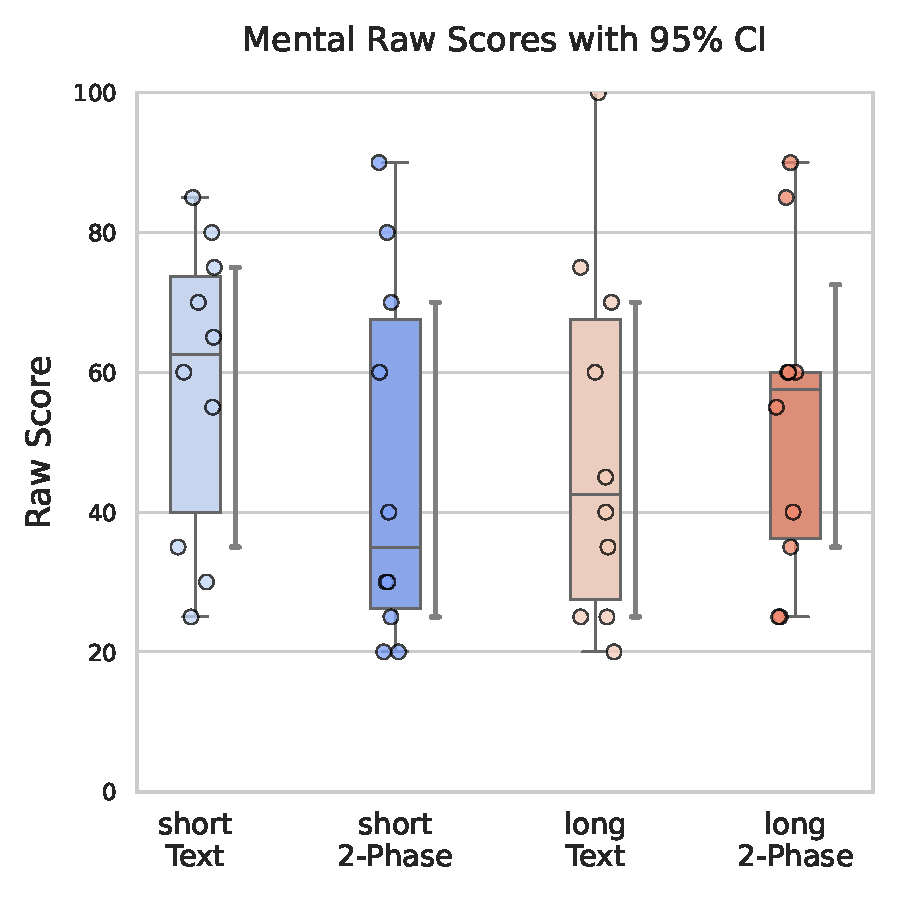
\includegraphics[width=\textwidth, trim=0 13 0 13, clip]{content/image/cog/Mental_scores.pdf}
        \caption{Mental Demand Raw Score: Across all four experiment groups, participants' reported mental demand is spread across a wide range with many participants experiencing high mental demand.}
        \Description{Box plot showing mental raw scores with 95\% confidence intervals across four interface versions: Short Text, Short 2-Phase, Long Text, and Long 2-Phase. The y-axis represents raw scores from 0 to 100. Each box plot includes individual data points. The Short Text and Short 2-Phase versions display wider score distributions, with medians around 60 and 40. The Long Text and Long 2-Phase versions have similar distributions but with slightly lower medians, 40 and 60, respectively. The plot shows a considerable spread in scores, with overlapping confidence intervals, indicating variability in mental demand across all groups.}
        \label{fig:mental_cog_score}
    \end{minipage}%
    \hfill
    \begin{minipage}[t]{0.32\textwidth}
        \centering
        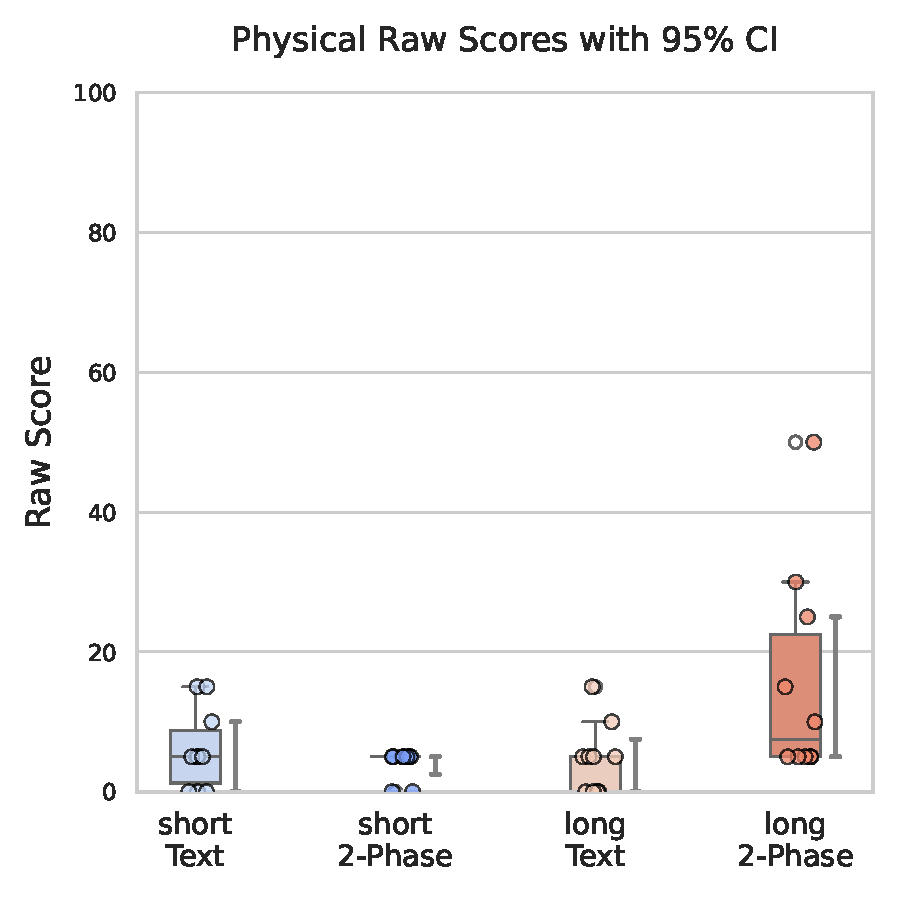
\includegraphics[width=\textwidth, trim=0 13 0 13, clip]{content/image/cog/Physical_scores.pdf}
        \caption{Physical Demand Raw Score: Participants other than the long two-phase interface reported minimal physical demand. The long two-phase interface had the highest physical demand, likely due to increased mouse clicks and extended time spent looking at the vertical screen.}
        \Description{A box plot showing the distribution of physical raw scores across four interface versions: Short Text, Short 2-Phase, Long Text, and Long 2-Phase. The y-axis represents the raw score ranging from 0 to 100. The box plots include individual data points, a central line for the median, and whiskers indicating the 95\% confidence interval. The Short Text, Short 2-Phase, and Long Text interfaces show minimal physical demand, with scores clustered below 20. The Long 2-Phase interface exhibits higher physical demand, with a few scores scattered up to around 60.}
        \label{apdxfig:physical_cog_score}
    \end{minipage}%
    \hfill
    \begin{minipage}[t]{0.32\textwidth}
        \centering
        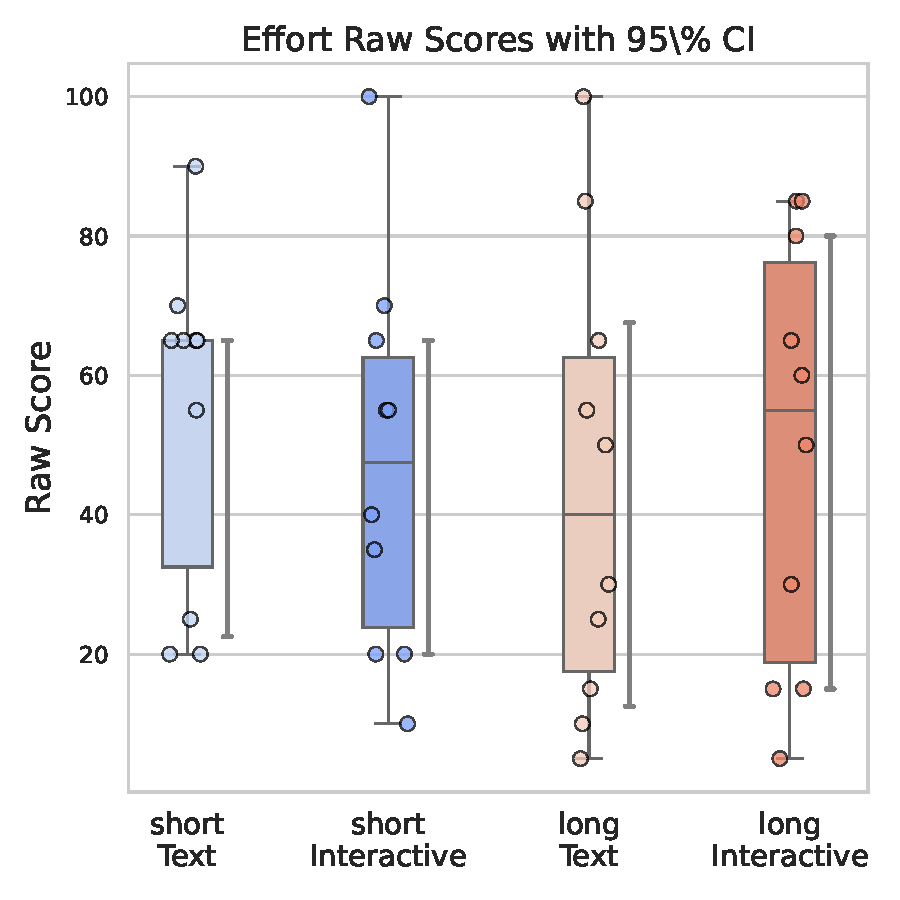
\includegraphics[width=\textwidth, trim=0 13 0 13, clip]{content/image/cog/Effort_scores.pdf}
        \caption{Effort Raw Score: Effort scores show indifference across groups. All groups had high variance of responses indicating some participants requires high amount of effort when completing QS regardless of length and interface}
        \Description{A box plot showing the distribution of effort raw scores across four interface versions: Short Text, Short 2-Phase, Long Text, and Long 2-Phase. The y-axis represents the raw score ranging from 0 to 100. Each box plot includes individual data points, a central line indicating the median, and whiskers representing the 95\% confidence interval. The Long 2-Phase interface shows the widest range of effort scores, while the other interfaces display more compact distributions. Data points are scattered within and outside the whiskers, reflecting variability in effort scores across the groups.}
        \label{apdxfig:effort_cog_score}
    \end{minipage}
\end{figure*}

\section{Detailed Qualitative Cognitive Load Breakdown}
\label{apdx:cog_qual}

In addition to the discussion on cognitive load sources presented in the main text, we provide additional details on the six cognitive dimensions. Among all dimensions, we also provide the codes representing different types of demand in a table form. The shaded cells represent the percentage of participants citing each source of mental demand, allowing for comparison within columns. The abbreviations in the columns: ST (Short Text Interface), S2P (Short Two-phase Interface), LT (Long Text Interface), and L2P (Long Two-phase Interface). Short and Long refer to the sum across both interfaces; Text and Inter refer to the sum across both survey lengths. We include Sparklines for comparisons across these experiment groups. Future studies can use these as initial codebooks to conduct interface studies on preference construction.

\begin{table*}[p]
   \caption{This table lists all the causes participants mentioned as contributing to their Mental Demand.}
   \Description{A table presenting mental demand across categories such as Budget Management (track credits, maximize usage), Preference Construction (prioritization, resource allocation), and Demand from Experiment Setup. Sparklines and percentage bars are used to visually represent the data across four interface versions (ST, S2P, LT, L2P) and experiment conditions (Short, Long, Text, Inter). The bars show higher mental demand in areas like Budget Management and Preference Construction, with trends highlighted by sparklines. Additional categories, such as External Factors and Demand due to Interface, are also represented with percentage bars.}
    \label{tbl:mental}
    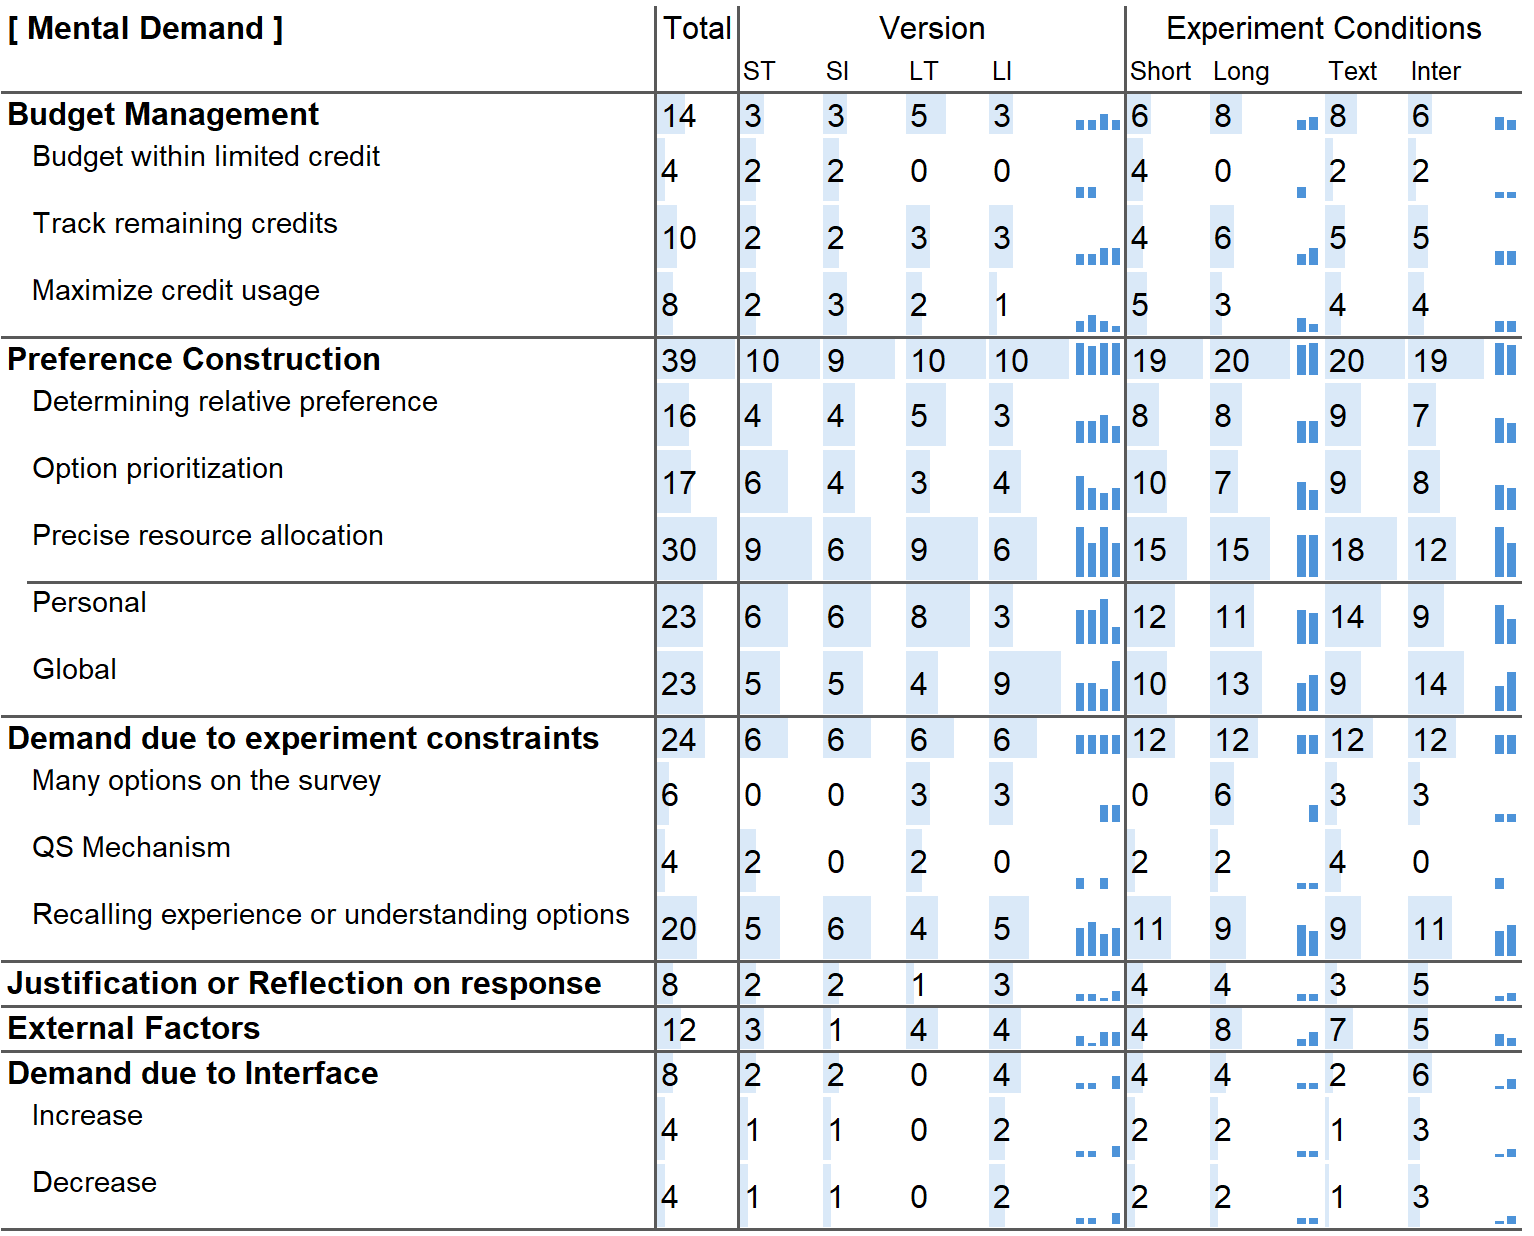
\includegraphics[width=0.78\linewidth]{content/image/cog/mental_table.png}
\end{table*}

\begin{table*}[p]
    \caption{Physical Demand Causes: Most participants expressed little or no physical demand. Results reflected that participants in the long two-phase interface required more actions, hence the higher mention of mouse usage as a source.}
    \Description{A table showing physical challenges experienced by participants, including Reading, Mouse, Vertical Screen, and None/Little physical effort, with sparklines and percentage bars visualizing the data trends. Data is split across four interface versions (ST, S2P, LT, L2P) and experiment conditions (Short, Long, Text, Inter). The Mouse category has the highest counts, with trends clearly visible via sparklines and bars, while Reading and Vertical Screen challenges have lower values. The None/Little row shows participants reporting minimal physical effort with percentage bars illustrating the distribution.}
    \label{apdx:physical_table}
    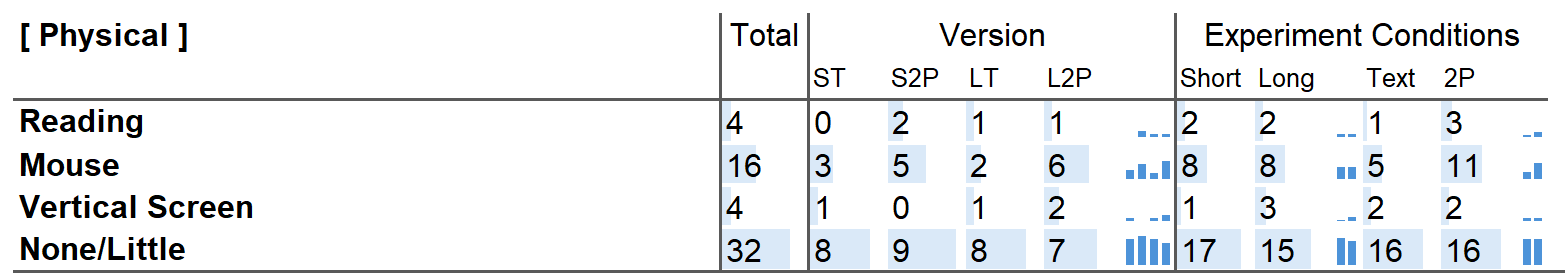
\includegraphics[width=0.78\linewidth]{content/image/cog/physical_table.png}
\end{table*}

\begin{table*}[p]
    \caption{Effort Sources: Participants using the text interface focused more on operational tasks, while those using the two-phase interface focused more on strategic planning.}
    \Description{A table summarizing participant effort as Operational and Strategic (personal and global), with data visualized using sparklines and percentage bars. The table is split into four versions (ST, S2P, LT, L2P) and experiment conditions (Short, Long, Text, Inter), with counts and corresponding bars for each category. The operational effort shows participants managing tasks, while the strategic effort captures balancing personal preferences with societal concerns. Sparklines highlight trends across different conditions. A None/Little/A bit row shows participants exerting minimal effort, visualized with bars.}

    \label{apdx:effort_table}
    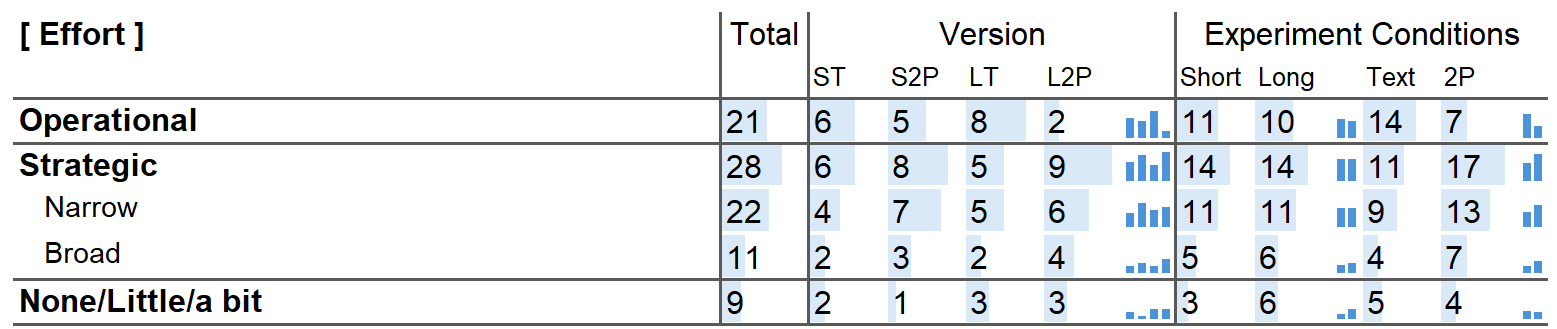
\includegraphics[width=0.78\linewidth]{content/image/cog/effort_table.png}
\end{table*}

\subsection{Sources of Mental Demand}
\label{apdx:mental}
Mental demand refers to the amount of mental and perceptual activity required to complete a task.~\Cref{tbl:mental} lists all qualitative codes and ~\Cref{fig:mental_cog_score} shows the boxplot of participant's subscale response. For thematic groups, we grouped them as source of demand (e.g., tracking remaining credits) and also of scope (e.g., Operational) as separated by the light gray line within each row.

\subsection{Sources of Physical Demand} 
\label{apdx:physical}
Physical demand refers to the physical effort required to complete a task, such as physical exertion or movement. Most participants reported minimal physical demand~($N=32$), reflected in the low NASA-TLX physical demand scores~(Figure~\ref{apdxfig:physical_cog_score}). Notably, $11$ out of $20$ participants who used the two-phase interface mentioned physical demand from using the mouse, reflecting interacting with two interfaces. This is further supported by the raw NASA-TLX physical demand scores~(Figure~\ref{apdxfig:physical_cog_score}), which show a significant visual difference between short and long two-phase interfaces as well as between text and two-phase interfaces in long surveys. Table~\ref{apdx:physical_table} presents all the relevant codes across experiment groups.




% \begin{figure}[t!]
%     \centering
%     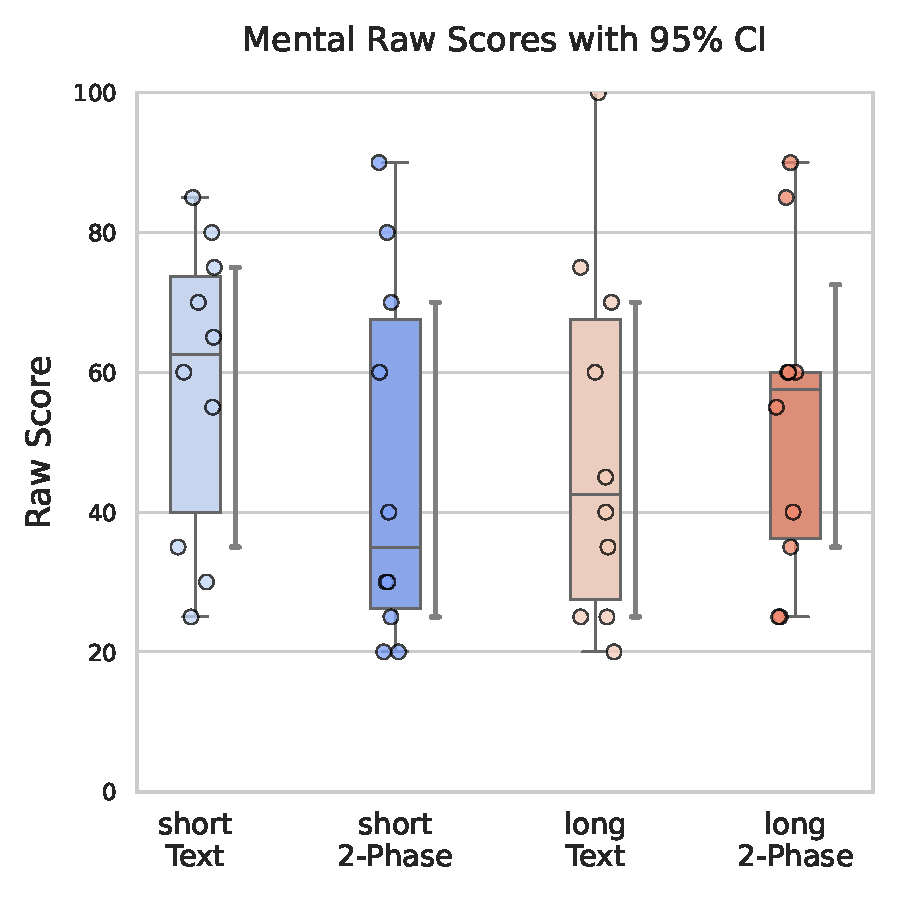
\includegraphics[width=0.38\textwidth, trim=0 13 0 13, clip]{content/image/cog/Mental_scores.pdf}
%     \caption{Mental Demand Raw Score: Across all four experiment groups, participants' reported mental demand is spread across a wide range with many participants experiencing high mental demand.}
%     \Description{Box plot showing mental raw scores with 95\% confidence intervals across four interface versions: Short Text, Short 2-Phase, Long Text, and Long 2-Phase. The y-axis represents raw scores from 0 to 100. Each box plot includes individual data points. The Short Text and Short 2-Phase versions display wider score distributions, with medians around 60 and 40. The Long Text and Long 2-Phase versions have similar distributions but with slightly lower medians, 40 and 60, respectively. The plot shows a considerable spread in scores, with overlapping confidence intervals, indicating variability in mental demand across all groups.}
%     \label{fig:mental_cog_score}
% \end{figure}

% \begin{figure}[h]
%     \centering
%     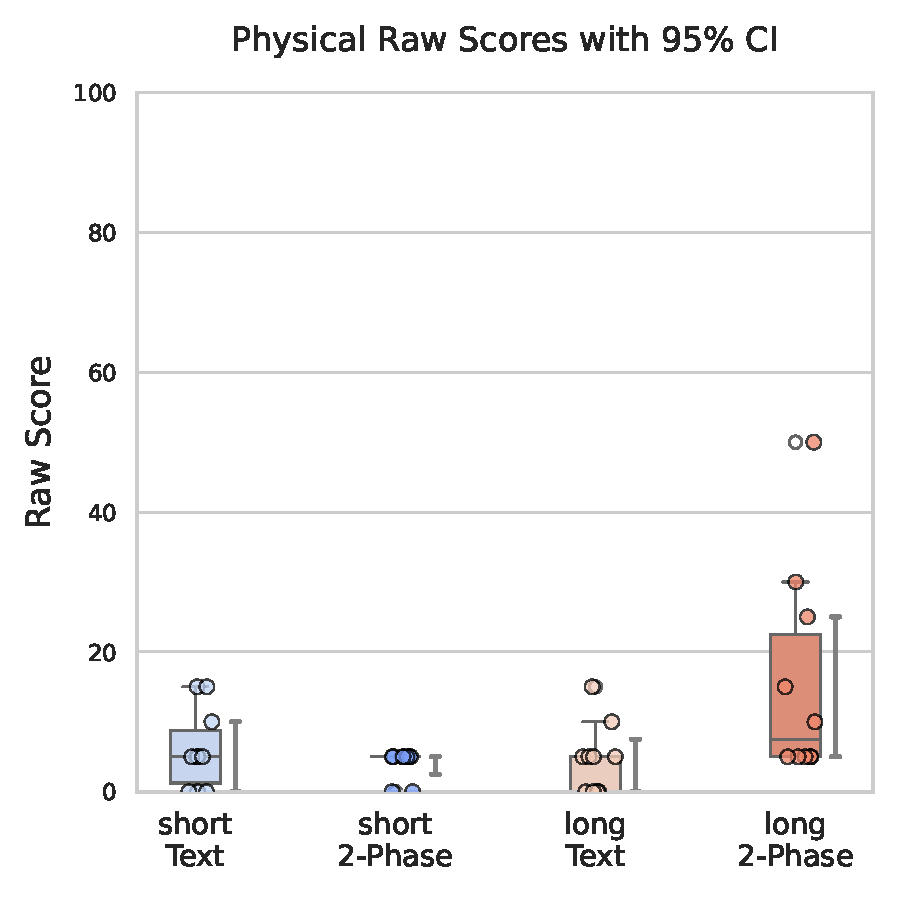
\includegraphics[width=0.38\textwidth, trim=0 13 0 13, clip]{content/image/cog/Physical_scores.pdf}
%     % \captionsetup{width=0.9\linewidth, justification=justified}
%     \caption{Physical Demand Raw Score: Participants other than the long two-phase interface reported minimal physical demand. The long two-phase interface had the highest physical demand, likely due to increased mouse clicks and extended time spent looking at the vertical screen.}
%     \Description{A box plot showing the distribution of physical raw scores across four interface versions: Short Text, Short 2-Phase, Long Text, and Long 2-Phase. The y-axis represents the raw score ranging from 0 to 100. The box plots include individual data points, a central line for the median, and whiskers indicating the 95\% confidence interval. The Short Text, Short 2-Phase, and Long Text interfaces show minimal physical demand, with scores clustered below 20. The Long 2-Phase interface exhibits higher physical demand, with a few scores scattered up to around 60.}
%     \label{apdxfig:physical_cog_score}
% \end{figure}

% \begin{figure}[h]
%     \centering
%     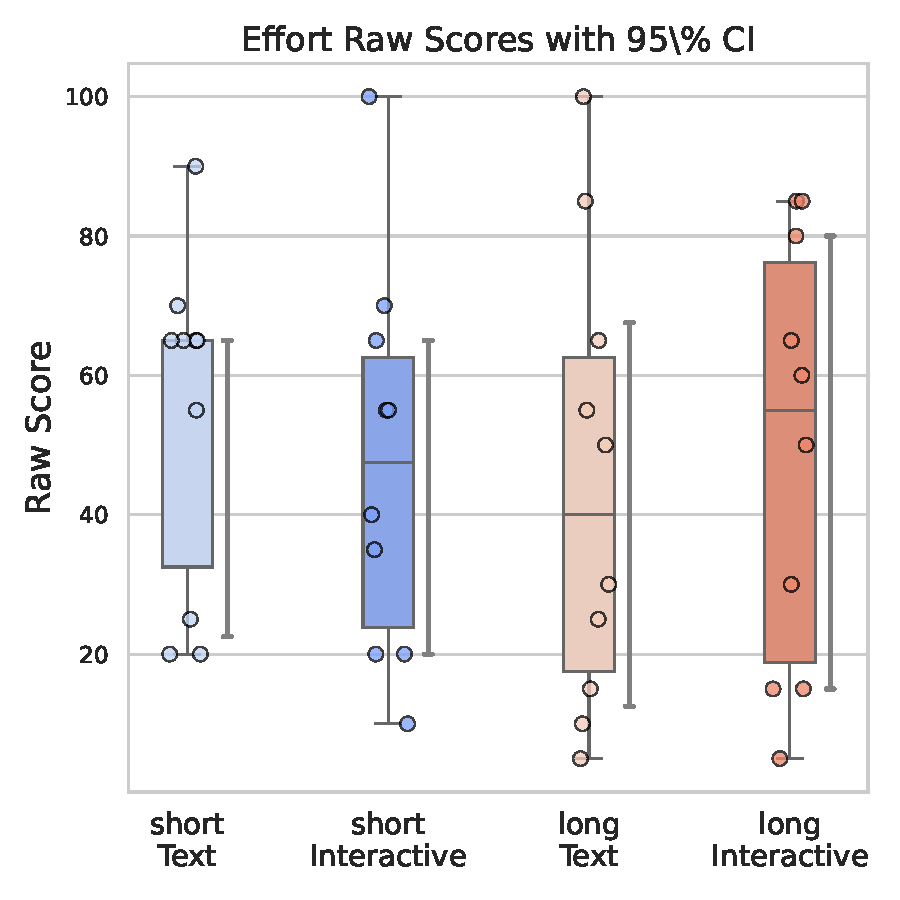
\includegraphics[width=0.38\textwidth, trim=0 13 0 13, clip]{content/image/cog/Effort_scores.pdf}
%     % \captionsetup{width=0.9\linewidth, justification=justified}
%     \caption{Effort Raw Score: Effort scores show indifference across groups.}
%     \Description{A box plot showing the distribution of effort raw scores across four interface versions: Short Text, Short 2-Phase, Long Text, and Long 2-Phase. The y-axis represents the raw score ranging from 0 to 100. Each box plot includes individual data points, a central line indicating the median, and whiskers representing the 95\% confidence interval. The Long 2-Phase interface shows the widest range of effort scores, while the other interfaces display more compact distributions. Data points are scattered within and outside the whiskers, reflecting variability in effort scores across the groups.}
%     \label{apdxfig:effort_cog_score}
% \end{figure}



% ============================================= %

\begin{table*}[p]
    \caption{Performance Causes: Most causes are shared across experiment conditions. We provided qualitative interpretations of their own performance assessments.}
    \Description{A table detailing participant performance across Operational Action (budget control, preference reflection, limited resources), Social Responsibility (decision maker, outcome uncertainty), and Performance Assessment (did their best, feel good, good enough). The table includes sparklines and percentage bars to visualize the distribution of performance data across four interface versions (ST, S2P, LT, L2P) and experiment conditions (Short, Long, Text, Inter). Operational action and social responsibility are visually represented, with sparklines highlighting performance trends.}

    \label{tbl:physical}
    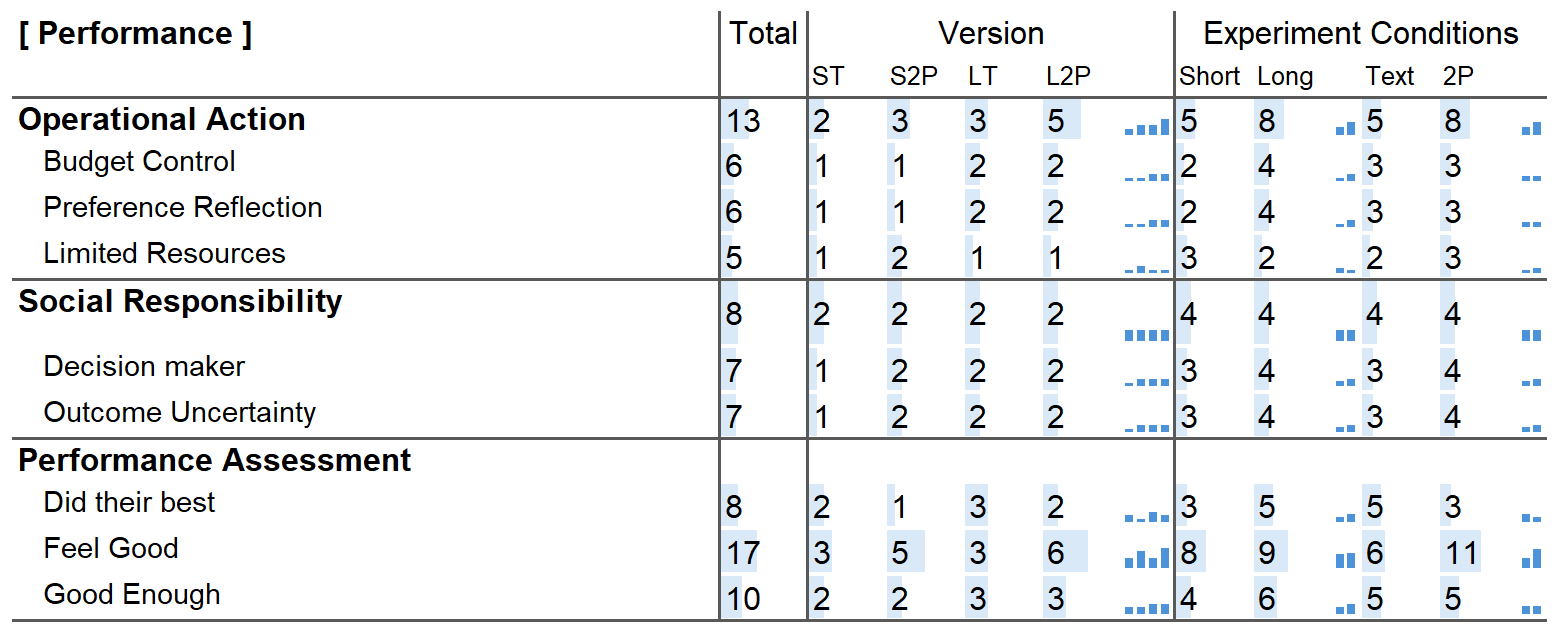
\includegraphics[width=0.7\linewidth]{content/image/cog/perf_table.png}
\end{table*}
\begin{table*}[p]
    \caption{Temporal Demand Sources: Decision-making and Operational Tasks are the main causes. Participants framed their decision-making sources differently.}
    \Description{A table categorizing temporal challenges across Budget Management, Decision Making (affirmative and negative), and Operational (task completion, efficiency). The data includes sparklines and percentage bars to visualize patterns across four versions (ST, S2P, LT, L2P) and experiment conditions (Short, Long, Text, Inter). Affirmative decision-making shows higher values than negative decision-making, with percentage bars indicating the relative distribution. Temporal operational tasks show consistent effort across conditions, as reflected in the sparklines.}

    \label{tbl:temporal}
    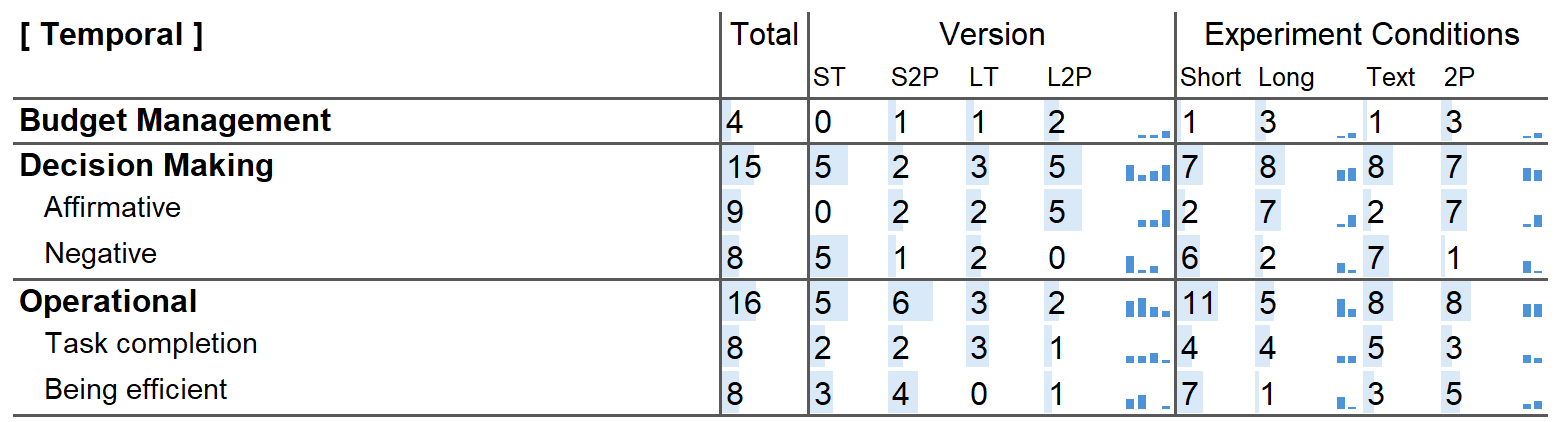
\includegraphics[width=0.7\linewidth]{content/image/cog/temporal_table.png}
\end{table*}


\subsection{Source of Effort}
\label{apdx:effort}
Effort refers to how hard participants felt they worked to achieve the level of performance they did. Since effort includes both mental and physical resource intensity, refer to \Cref{apdx:mental} and \Cref{apdx:physical} for definitions. Raw NASA-TLX effort scores~(Figure~\ref{apdxfig:effort_cog_score}) showed a similar spread across experiment groups, the qualitative analysis showed more distinction that participants using the two-phase interface considered options more comprehensively and felt less effort on completing operational tasks, similar to what we found on mental demands~(Section \ref{apdx:mental}). Table~\ref{apdx:effort_table} contains codes.

\subsubsection{Effort Source \#1: Operational Tasks} $14$ of the $20$ participants using the text interface mentioned Operational Tasks as effort sources, compared to $7$ using the two-phase interface, with the lowest mention by the long two-phase interface group~($N=2$). Quotes below illustrated participants putting in effort to manipulate the interface.
\begin{displayquote}
I wanted to bump up~(an option) maybe to 4 or <option> to 5 and realize I couldn't.~\bracketellipsis that would be effort came in of how do I want to really rearrange this to make it~(the budget spending) maximize?

\noindent \hfill -- S029, short text interface
\end{displayquote}
\begin{displayquote}
So it was like it was very~\ldots I have to put a lot of effort in terms of you know~\ldots think about each dimension that if I give one credit to <option name> whether it will affect my credits on <another option name>. 

\noindent\hfill -- S005, long text interface
\end{displayquote}

\subsubsection{Effort Source \#2: Strategic Planning} Different from Operational Tasks, $11$ participants in the text interface compared to $17$ participants described strategic planning as sources of effort, with almost all participants~($N=9$) from the long two-phase interface. We further categorize strategic planning into \textit{narrow} and \textit{broad} scopes as we did for mental demand~\cref{sec:mental}. Participants using the two-phase interface~($N=7$) had nearly mentioned double~($N=4$) times regarding global strategies. For example:

\begin{displayquote}
And really the bulk of the effort was how to rank order these~(options) and allocate the resources behind the upvotes so that I can accurately depict what I want~\ldots say, a committee to focus on and allocate actual fungible resources, too. \noindent \hfill -- S019, long two-phase interface
\end{displayquote}




\begin{table*}[p]
    \caption{Frustration Sources: Frustration comes from different levels of strategic operations or operational tasks.}
    \Description{A table with sparklines showing frustration categories: Strategic (higher-level and lower-level) and Operational, across four versions (ST, S2P, LT, L2P) and experiment conditions (Short, Long, Text, Inter). The table includes sparklines and percentage bars alongside the numerical counts to visually represent the data distribution across conditions. Strategic frustration is divided into higher-level and lower-level conflicts between personal preference and broader societal values. Operational frustration includes challenges such as credit management, adhering to the quadratic mechanism, making decisions, and understanding options. A final row captures participants reporting None/Little frustration, also visualized with percentage bars.}

    \label{tbl:fustration}
    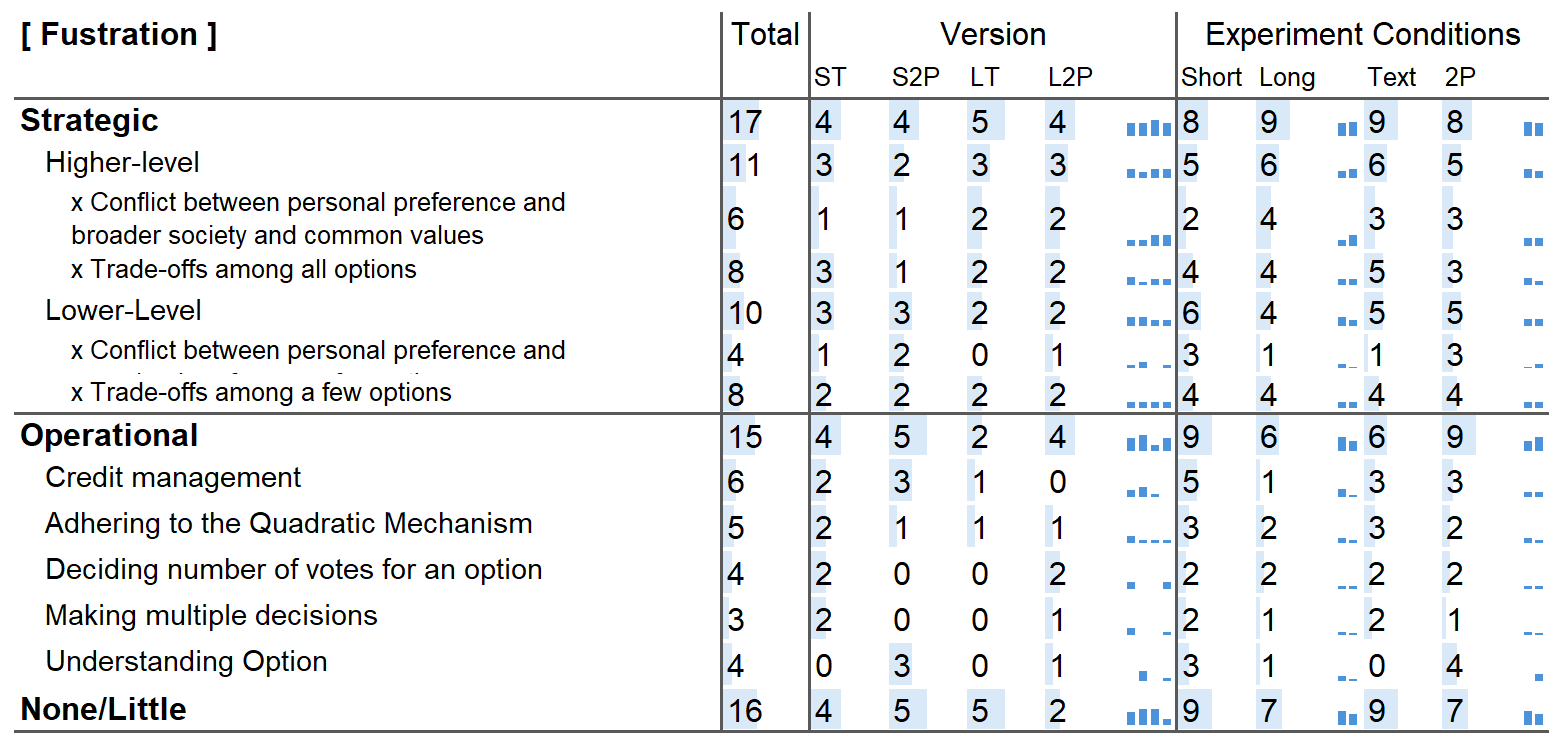
\includegraphics[width=0.7\linewidth]{content/image/cog/fustration_table.png}
\end{table*}

\subsection{Source from Performance}
\label{apdx:performance}

Performance refers to a person's perception of their success in completing a task. Lower values mean good perceived performance; higher values mean poor perceived performance. We found minimal qualitative differences between experiment groups regarding factors influencing perceived performance. Two influencing factors emerged: \textit{Operational Actions} and \textit{Social Responsibility}. Despite most participants reporting positively on their performance, nuances exist in how different groups interpret their performance.

\subsubsection{Operational Actions}
Operational actions, like the theme presented in temporal demand, refer to specific, executable procedures participants perform in the survey. This could involve: pressure to spend all credits or stay within budget~($N=6$), fears that final vote choices did not reflect true preferences($N=5$), or concerns that they had finished the task inefficiently~($N=6$).


\subsubsection{Social Responsibility}
Social responsibility-based concerns around performance came up when participants reflected on how their final vote counts would be perceived by others~(\smallquote{S041}{I don't want people to think that I just like don't care about <ethnicity> people at all}) or influence real-world decision-making~(\smallquote{S027}{Some of these things might \ldots have outcomes that I didn't foresee}).

All groups cited social responsibility as source to evaluate effort. Raw NASA-TLX scores~(Figure~\ref{fig:performance_cog_score}) show participants had indistinguishable performance scores. This aligns with the interview results where most participants felt positive about their final submission. 

To dig deeper, we also analyzed participants' language when they described their performance. Expressions like ``good enough'' may be indicative of satisficing behaviors -- our results suggest participants are satisfied at similar rates regardless of the interface. 1/4 of the participants in the text interface expressed ``done their best,'' referring to exhausting their effort. Participants who used a two-phase interface were generally more positive about their final outcome -- they were twice as likely to report "feeling good" about their final results~($N=11$ v.s. $N=6$).

\begin{figure}[h]
    \centering
    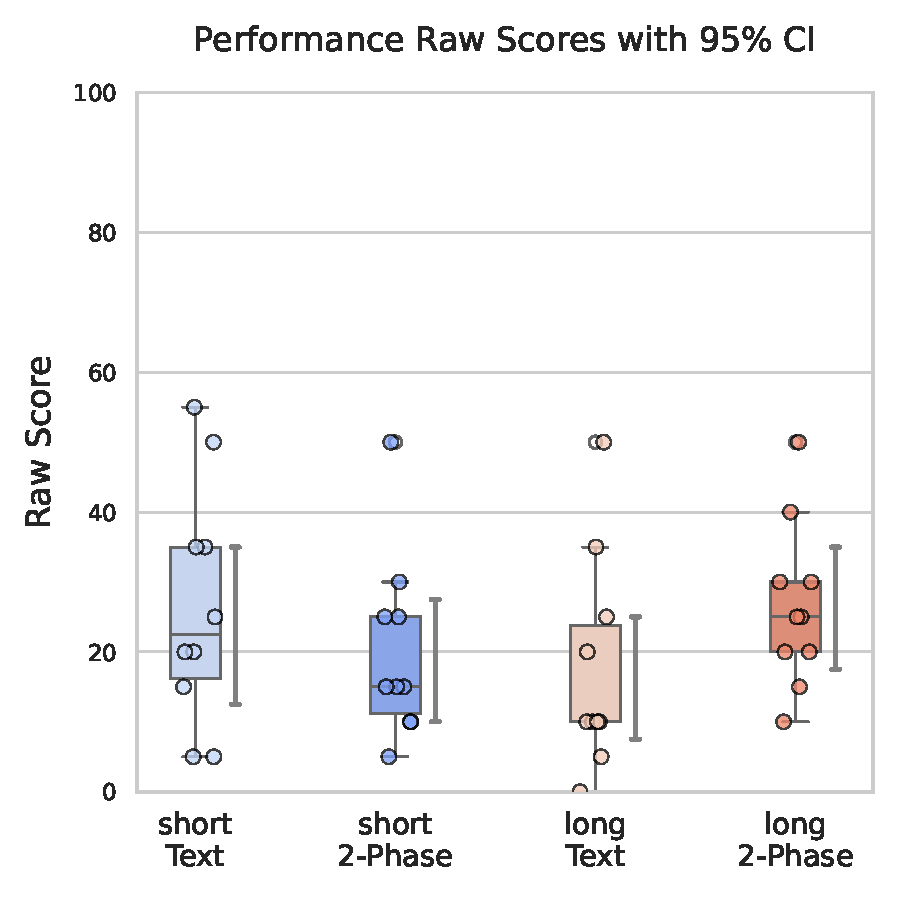
\includegraphics[width=0.38\textwidth, trim=0 13 0 13, clip]{content/image/cog/Performance_scores.pdf}
    \captionsetup{width=0.9\linewidth, justification=justified}
    \caption{Performance Demand Raw Score: Participants showed indifferent performance raw scores across experiment conditions, all trending toward satisfactory.}
    \Description{A box plot displaying the distribution of performance raw scores across four interface versions: Short Text, Short 2-Phase, Long Text, and Long 2-Phase. The y-axis represents raw scores ranging from 0 to 100. Each box plot includes individual data points, a central line for the median, and whiskers representing the 95\% confidence interval. The performance scores appear relatively low across all conditions, with medians hovering between 20 and 40.}
    \label{fig:performance_cog_score}
\end{figure}

\subsection{Temporal Demand}
Table~\ref{apdx:temporal_table} lists all the mental demand codes.
\label{apdx:temporal_table}


\subsection{Frustration}
Table~\ref{apdx:frus_table} lists all the mental demand codes.
\label{apdx:frus_table}

\begin{figure}[h]
    \centering
    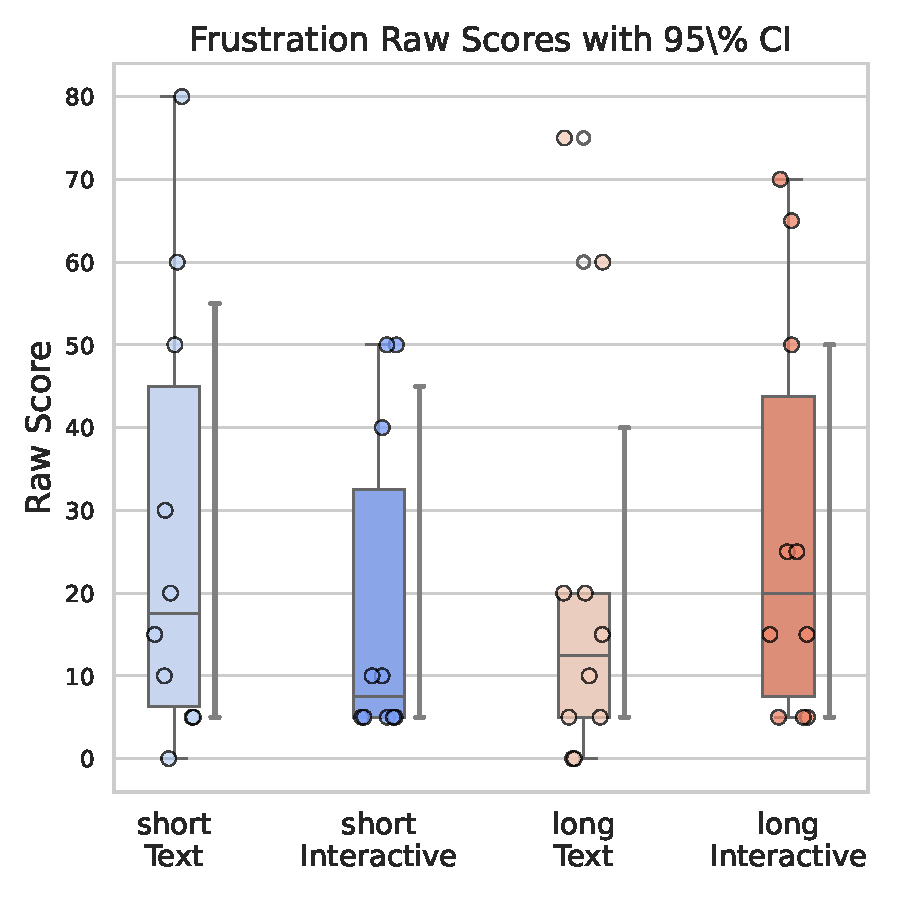
\includegraphics[width=0.38\textwidth, trim=0 13 0 13, clip]{content/image/cog/Frustration_scores.pdf}
    \captionsetup{width=0.9\linewidth, justification=justified}
    \caption{Frustration Raw Score: Participants other than the long text interface highlighted several operational tasks that led to frustration. All groups share causes from strategic planning.}
    \Description{Box plot showing frustration raw scores with 95\% confidence intervals across four interface versions: Short Text, Short 2-Phase, Long Text, and Long 2-Phase. The y-axis represents raw scores from 0 to 100. The Short Text interface has a wide range of scores, with several participants reporting high frustration. The Short 2-Phase interface shows lower median frustration with a narrower distribution. The Long Text interface displays the lowest frustration scores, while the Long 2-Phase interface shows a wide range, with some participants reporting high frustration. Individual data points are included, indicating variability across participants.}
    \label{fig:frustration_cog_score}
\end{figure}
% \section{Additional voting behavior data}
\label{apdx:additional_results_behavior}
In this section, we describe the additional voting behavior that we observed. The reason why we decided to focus on the percentage of remaining credits comes from prior literature `scarcity frames value'~\cite{Shah2015a}, a driver that makes researchers believe makes quadratic voting more accurate~\cite{chengCanShowWhat2021}. We did not follow ~\textcite{quarfoot2017quadratic} in counting accumulated votes over time due to varying total times across individuals.

We observed the number of vote adjustments given a remaining vote credit percentage. Figure~\ref{apdxfig:voting_all} showed all the voting actions over the remaining credit for the four experiment conditions. Here we see two distinct patterns between the short survey and the long survey in terms of participant behaviors. In long surveys, participants exhibited more actions both when the budget was abundant and when it began to run out. This pattern was more pronounced with the long two-phase interface. This difference is why we further focused on the long QS group.

\begin{figure}[ht]
    \centering
    \includegraphics[width=\textwidth]{content/image/results/clickstream_action_distribution.pdf}
    \caption{This plot counts the number of voting actions when there are $x$ percentages of credits remaining. A KDE plot is provided to help better understand the action distribution.}
    \Description{A four-panel histogram showing the number of voting actions across remaining credit percentages for four interface versions: Short Text, Short 2-Phase, Long Text, and Long 2-Phase. Each panel displays the number of actions on the y-axis and remaining credit on the x-axis, with an overlaid KDE curve representing density. In the top panels (Short Text and Short 2-Phase), actions are distributed relatively evenly, with small peaks around 10-20\% and 50\% remaining credit. The KDE curves show minor fluctuations. In the bottom panels (Long Text and Long 2-Phase), there are more pronounced peaks at 0-10\% and 100\% remaining credit, with broader distributions and smoother KDE curves indicating denser actions around these areas. The Long Text and Long 2-Phase interfaces exhibit more actions overall compared to the Short Text and Short 2-Phase interfaces.}
    \label{apdxfig:voting_all}
\end{figure}

Figure~\ref{apdxfig:voting_v3_v4} presents the comparison between when participants make small or large vote adjustments at different budget levels. Revisiting the KDE curve in the second row in Figure~\ref{apdxfig:voting_all} and the curve of the second row in Figure~\ref{apdxfig:voting_v3_v4} show a stronger bimodal distribution for small vote adjustments across interfaces. In fact, the bimodal distribution is more pronounced in the two-phase interface. This suggests that participants make small adjustments both at the beginning and toward the end of the QS. However, the two-phase interface shows more frequent and faster edits towards the end. In comparison, participants also made more large vote adjustments early on that spread more equally compared to the text interface. This indicates that participants had a clearer idea of how to distribute their credits across the options.

\begin{figure}[ht]
    \centering
    \includegraphics[width=\textwidth]{content/image/results/combined_density_plots.pdf}
    \caption{This plot further separates participants' interaction behavior based on the number of votes participants adjusted. We observed a bimodal interaction pattern across long QS when small vote adjustments are made.}
    \Description{A four-panel plot comparing the time to take action in seconds over remaining credit percentages for large and small vote adjustments in the Long Text and Long 2-Phase interfaces. Each panel includes scattered points and an overlaid KDE curve. The top left panel shows large vote adjustments for the Long Text interface, with peaks in the KDE curve around 20\% and 80\% remaining credit. The top right panel shows large vote adjustments for the Long 2-Phase interface, with two peaks in the KDE curve around 10\% and 100\%. The bottom left panel shows small vote adjustments for the Long Text interface, with scattered points and peaks in the KDE curve around 10\% and 90\%. The bottom right panel shows small vote adjustments for the Long 2-Phase interface, with a KDE curve peaking around 10\% and 100\% remaining credit. Box plots on the right side of each panel summarize the distribution of time taken to adjust votes for each interface.}    
    \label{apdxfig:voting_v3_v4}
\end{figure}



% Modeling Appendix
\section{Modeling}
\section{Modeling NASA-TLX Weighted Scores and Subscales}
In this section, we first describe the modeling approach for the NASA-TLX weighted scores and subscales, and then present all subscale results.

\subsection{Modeling Approach}
We modeled the NASA-TLX weighted scores and subscales using a hierarchical Bayesian ordinal regression model. 

\subsubsection{Dependent variables}
\paragraph{NASA-TLX weighted scores} are transformed from a continuous $0$–$100$ scale to cognitive levels: low, medium, somewhat high, high, and very high, as described by~\textcite{hart1988development}. This transformation helps the model adapt to sparse data. In our study, there were no participants who expressed "low" or "very high"; thus, we modeled the predictive variables as "medium," "somewhat high," and "high."

\paragraph{NASA-TLX subscale ratings} are transformed into ordinal groups using using minimum frequency binning~\cite{frank2001simple}. Minimum frequency binning involves grouping adjacent response categories until each bin meets a predefined minimum number of observations. The subscale uses a 21-point Likert scale, with 40 participants, it makes the ordinal data very sparse. Minimum frequency binning mitigates this allowing similiar number of participants in each bin. We applied weighted bins across all participants within the same subscale, ensuring that each bin contained at least 10 participants.

\subsubsection{Independent Variables}
For this model, we used three independent variables: length ($\gamma_i$), interface type ($\beta_I$), and the interaction between the two ($\phi_{ij}$). Length, categorized as "low" and "short," was modeled as an ordinal variable, as shown in Equation~\ref{eq:cog_ordinal}. Since there are only two categories, this approach allowed us to model the baseline length effect and the added effect of the longer length. Interface types were set up with hyperpriors, from which the interfaces were drawn. The interaction effect used a non-centered parameterization constrained by an LKJ prior to account for correlations, as described in Equation~\ref{eq:cog_lkj}.

\subsubsection{Overall model}
We modeled the dependent variables using an Ordered Logistic (Equation~\ref{eq:cog_main}). The observed outcome variable $y_i$, represents the response for the $i$-th observation parameterized by the latent predictor $\eta_i$ and thresholds $\tau$. An intuitive way to understand this is that the model attempts to learn $\eta_i$ through a regression and the cutpoints $\tau$ to transform it into ordinal outcomes, similar to how we created the ordinal outcome variables. $\eta_i$ is described in Equation~\ref{eq:cog_regression}.


\begin{align}
    y_i &\sim \text{OrderedLogistic}(\eta_i, \boldsymbol{\tau}) \label{eq:cog_main}\\
    \eta_i &= \alpha + \gamma_i + \beta_I[I_i] + \phi_{ij} \label{eq:cog_regression}\\
    \boldsymbol{\tau} &\sim \text{OrderedTransform}(\mathcal{N}(0, 1)^{K-1}) \\
    \gamma_i &= \mu_L + \beta_L \cdot L_i \label{eq:cog_ordinal} \\
    \phi_{ij} &= L_{\Omega} \cdot (\sigma_{\phi} \odot z_{\phi}) \label{eq:cog_lkj}
\end{align}


\paragraph{We describe the priors used:}
\begin{align}
    \mu_{L}, \mu_{\beta_L}, \mu_{\beta_I} &\sim \mathcal{N}(0, 1), \quad \sigma_{\beta_L}, \sigma_{\beta_I} \sim \text{Exponential}(1) \label{eq:cog_prior_1} \\
    \beta_L &\sim \mathcal{N}(\mu_{\beta_L}, \sigma_{\beta_L}), \quad \beta_I \sim \mathcal{N}(\mu_{\beta_I}, \sigma_{\beta_I}) \label{eq:cog_prior_2} \\
    L_{\Omega} &\sim \text{LKJ}(2), \quad \sigma_{\phi} \sim \text{Exponential}(1), \quad z_{\phi} \sim \mathcal{N}(0, 1) \label{eq:cog_prior_3} 
\end{align}

\subsubsection{Model Results}
We conducted the Bayesian analysis using NumPyro, a widely used framework for Bayesian inference. We used Markov Chain Monte Carlo (MCMC) sampling, a method commonly applied in Bayesian inference. All the models showed that the Gelman-Rubin statistic ($\hat{R}$) parameters were equal to 1 across two chains, indicating that the multiple sampling chains converged. We present each subscale result and provide a short description of these results.

% Section for Mental subscale
\subsubsection{Mental Subscale}
Figure~\ref{fig:bayesian_mental_subscale} shows pairwise bayesian results from mental demand highlighted 70.4\% of posterier probaility that participants in the long two-phase condition had a higher mental demand compared to the short two-phase condition. On the other hand, the short text condition had a 74.5\% posterior probability of having a higher mental demand compared to the short two-phase condition. This is additional evidence that prompted us to believe that the participants in the short two-phase participants benifited from the organization phase. The sheer number of added options in the long two-phase condition may have added additional demand to participants, leading to higher mental demand.

\begin{figure}[h!]
    \centering
    \includegraphics[width=\textwidth]{content/image/cog/Mental_cog_diff_single_row.pdf}
    \caption{Differences in the mental subscale scores by version.}
    \label{fig:bayesian_mental_subscale}
\end{figure}

% Section for Physical subscale
\subsubsection{Physical Subscale}
Figure~\ref{fig:bayesian_physical_subscale} shows the pairwise comparison of the physical subscale. Noteable results shows that there is a 86.1\% posterior probability that the long text condition had a lesser physical demand compared to the short text condition. This is counter intuitive as the long text participants actually traversed much higher edit distances. We are not clear what prompted their self reported value and requires future research. 

\begin{figure}[h!]
    \centering
    \includegraphics[width=\textwidth]{content/image/cog/Physical_cog_diff_single_row.pdf}
    \caption{Differences in the physical subscale scores by version.}
    \label{fig:bayesian_physical_subscale}
\end{figure}

% Section for Temporal subscale
\subsubsection{Temporal Subscale}
Figure~\ref{fig:bayesian_temporal_subscale} shows the pairwise comparison of the temporal subscale. The results show that the long two-phase condition once again had a 74.6\% posterior probability of having a lower temporal demand compared to the short text condition. Conversely, participants in the long two-phase condition had a 71.1\% posterior probability of having a higher temporal demand compared to the short two phase condition, reflecting the longer time they took to complete the survey questions. We believe that the lower temporal demand in the long two-phase condition are potential indicators of participant's satisficing behavior.

\begin{figure}[h!]
    \centering
    \includegraphics[width=\textwidth]{content/image/cog/Temporal_cog_diff_single_row.pdf}
    \caption{Differences in the temporal subscale scores by version.}
    \label{fig:bayesian_temporal_subscale}
\end{figure}

% Section for Performance subscale
\subsubsection{Performance Subscale}
We omit the pairwise comparison of the performance subscale due to the mixed signals. We focused on the qualitative results analyzed in the main text.
% Figure~\ref{fig:bayesian_performance_subscale} shows the pairwise comparison of the performance subscale. The results showed mixed signals. Thus, we focused on the qualitative results analyzed in the main text.

% \begin{figure}[h!]
%     \centering
%     \includegraphics[width=\textwidth]{content/image/cog/Performance_cog_diff_single_row.pdf}
%     \caption{Differences in the performance subscale scores by version.}
%     \label{fig:bayesian_performance_subscale}
% \end{figure}

% Section for Effort subscale
\subsubsection{Effort Subscale}
We omit the pairwise comparison of the effort subscale due to its similarity to the mental demand subscale. 

% \begin{figure}[h!]
%     \centering
%     \includegraphics[width=\textwidth]{content/image/cog/Effort_cog_diff_single_row.pdf}
%     \caption{Differences in the effort subscale scores by version.}
%     \label{fig:bayesian_effort_subscale}
% \end{figure}

% Section for Frustration subscale
\subsubsection{Frustration Subscale}
Figure~\ref{fig:bayesian_frustration_subscale} shows the pairwise comparison of the frustration subscale. The results show that the long two-phase condition had a 68.3\% posterior probability of having a higher frustration compared to the short two-phase condition, likey due to the added number of options to assess. 

\begin{figure}[h!]
    \centering
    \includegraphics[width=\textwidth]{content/image/cog/Frustration_cog_diff_single_row.pdf}
    \caption{Differences in the frustration subscale scores by version.}
    \label{fig:bayesian_frustration_subscale}
\end{figure}

\section{Modeling edit distance} \label{sec:apdx:model_distance}
In this section, we describe the details for the three models we used to analyze the edit distance data.

\subsection{Model 1: Edit Distance per Option} \label{sec:apdx:model_distance_option}

\subsubsection{Dependent variables}
The dependent variable for this model is the edit total distance accumulated for an option $D_i$. Distance is a positive continuous variable.

\subsubsection{Independent variables}
The independent variables for this model are the length of the option $L_i$, modeled as a ordinal variable (Equation~\ref{eq:distance_model_1_eta_ordinal}); interface type $I_i$, modeled as a categorical variable; user effect $U_i$ as categorical variables. The ordinal variable $L_i$ consists of a intercept $\mu_L$ and added effect $\beta_L$, given the interface ordinal value. Since we only have two interfaces, we do not have to worry about the interval between two or more interfaces. Priors are weakly informed in Equation~\ref{eq:priors_global_mean}. We reparamtereized $U_i$ given the sparser sample from each participant. This is written in Equations~\ref{eq:distance_model_1_user_effect}. Both reparameterization contains an intercept and scaling of the effect due to this user. This will imporve sampling efficiency and help the model converge. Relavent priors are written in Equations~\ref{eq:priors_global_mean} and~\ref{eq:priors_sigma_U}. We added an interaction effect between length and interface type $\phi_{ij}$ described in Equation~\ref{eq:distance_model_1_lkj}. Similiar to cognitive load model, the interaction effect used a non-centered parameterization constrained by an LKJ prior to account for correlations. Priors for the interaction effect is listed in Equations~\ref{eq:priors_sigma_phi} and~\ref{eq:priors_L_Omega}. Detailed description can be found in Appendix~\ref{apdx:model_tlx}.

\subsubsection{Overall model and Likelihood function}
We modeled the dependent variable using an Exponential distribution (Equation~\ref{eq:distance_model_1}). Since Exponential distribution takes in a positive value, we transformed it as Equation~\ref{eq:transformation_model_1}. The observed outcome variable $D_i$ represents the response for the $i$-th observation parameterized by the latent predictor $\eta_i$. $\eta_i$ is described in Equation~\ref{eq:distance_model_1_eta} as the regression with length, interface, the interaction effect and the interface.

\begin{align}
    D_i \sim \text{Exponential}(\lambda_i) \label{eq:distance_model_1} \\
    \lambda_i = \exp(\eta_i) \label{eq:transformation_model_1}\\
    \eta_i = \gamma_i + \beta_I[I_i] + \phi_{ij} + U_i \label{eq:distance_model_1_eta} \\
    \gamma_i = \mu_L + \beta_L \cdot L_i \label{eq:distance_model_1_eta_ordinal} \\
    \phi_{ij} = L_{\Omega} \cdot (\sigma_{\phi} \odot z_{\phi}) \label{eq:distance_model_1_lkj} \\
    U_i = \mu_U + \sigma_U \cdot z_U \label{eq:distance_model_1_user_effect}
\end{align}

Priors are defined as:
\begin{align}
    \mu_L, \mu_I, \mu_U, \beta_L, \beta_I, z_{\phi}, z_U &\sim \mathcal{N}(0, 1) \label{eq:priors_global_mean} \\
    \sigma_{\phi} \sim \text{HalfNormal}(0.5) \label{eq:priors_sigma_phi} \\
    \sigma_U \sim \text{Exponential}(0.5) \label{eq:priors_sigma_U} \\
    L_{\Omega} \sim \text{LKJ}(3) \label{eq:priors_L_Omega}
\end{align}

\subsection{Model 2: Edit Distance with Separate Mean and Variance Predictors} \label{sec:apdx:model_distance_variance}

\subsubsection{Dependent Variables}
The dependent variable for this model is the edit distance (with directions) $D_i$, a positive edit distance refers to participants moving downward. A negtaitve edit distrance refers to a upward movement.

\subsubsection{Overall Model}
We modeled the dependent variable $D_i$ using a Normal distribution (Equation~\ref{eq:distance_model_2_likelihood}). Since the goal of this model, unlike some, aims to model the variance since we believe participants in two-phase interface would exhibit less oscillation then the text interface. Hence, we model independent variables effecting both $\mu$ and $\sigma$ independently for this analysis to exaime this hypothesis.

\subsubsection{Independent Variables}
The independent variables for this model are:
\begin{itemize}
    \item \textbf{Length of the option $L_i$}: Modeled as an ordinal variable. Since we will be modeling both $\mu_i$ and $\sigma$ of a Normal distribution, Equation~\ref{eq:distance_model_2_gamma_mu} and ~\ref{eq:distance_model_2_gamma_sigma} reflects the ordinal variable. Both formula consists of a intercept $\mu_{L,\mu}, \mu_{L,\sigma}$ and added effect $\beta_{L,\mu}, \beta_{L,\sigma}$, given the interface ordinal value. Since we only have two interfaces, we do not have to worry about the interval between two or more interfaces. Priors of both ordinal relationship are weakly informed in Equation~\ref{eq:priors_distance_model_2_mean} and~\ref{eq:priors_distance_model_2_variance}
    \item \textbf{Interface type $I_i$}: Modeled as a categorical variable. Following the previous discussion, they are drawn from a hyperprior. We reparamtereized this independent variable given the added complexity of this model. This is written in Equations~\ref{eq:distance_model_2_beta_I_mu} and~\ref{eq:distance_model_2_beta_I_sigma}. Both reparameterization contains an intercept and scaling of the effect due to this interface. Relavent priors are written in Equations~\ref{eq:priors_distance_model_2_mean},~\ref{eq:priors_distance_model_2_variance}, and~\ref{eq:priors_interface_distance_model_2}.
    \item \textbf{User effect $U_i$}: Users are modeled as categorical variables. Following the interface, it is also reparamtereized as Equations~\ref{eq:distance_model_2_user_mu} and~\ref{eq:distance_model_2_user_sigma}. Priors are defined in Equations~\ref{eq:priors_distance_model_2_mean},~\ref{eq:priors_distance_model_2_variance}, and~\ref{eq:priors_sigma_U_distance_model_2}
    \item \textbf{Interaction between length and interface type $\phi_{ij}$}: Similiar to the interaction effect for cognitive load, we used a non-centered parameterization constrained by an LKJ prior to account for correlations. This is described by Equation~\ref{eq:distance_model_2_phi_mu} and~\ref{eq:distance_model_2_phi_sigma}. Refer to Appendix~\ref{apdx:model_tlx} for a more detailed explaination. Relevent priors are described in Equation~\ref{eq:priors_L_Omega_distance_model_2} and~\ref{eq:priors_sigma_phi_distance_model_2}. We relaxed the LKJ priors comapred to the cognitive load model given the complexity of the model allowing a lesser belief in correlation among the two variables.
\end{itemize}

\subsubsection{Likelihood Function}
Given these independent variables, we model both $\mu$ and $\sigma$ as linear regressions. While we can directly model $mu$ (Equation~\ref{eq:distance_model_2_mu}), we need to make sure $sigma$ is strictly positive, we applied a transformation described in~\ref{eq:distance_model_2_sigma}. Hence, both $\mu_i$ and $\log(\sigma_{\text{obs},i})$ now regresses on the linear combination of length, interface, interaction effect, and user effect. 

\begin{align}
    D_i &\sim \text{Normal}(\mu_i, \sigma_{\text{obs},i}) \label{eq:distance_model_2_likelihood} \\
    \mu_i &= \gamma_{\mu,i} + \beta_{I,\mu}[I_i] + \phi_{\mu,ij} + U_{\mu,i} \label{eq:distance_model_2_mu} \\
    \gamma_{\mu,i} &= \mu_{L,\mu} + \beta_{L,\mu} \cdot L_i \label{eq:distance_model_2_gamma_mu} \\
    \beta_{I,\mu}[I_i] &= \mu_{I,\mu} + \sigma_{I,\mu} \cdot \text{I}_{\mu,I_i} \label{eq:distance_model_2_beta_I_mu} \\
    \phi_{\mu,ij} &= L_{\Omega,\mu} \cdot (\sigma_{\phi,\mu} \odot z_{\phi,\mu}) \label{eq:distance_model_2_phi_mu} \\
    U_{\mu,i} &= \mu_{U,\mu} + \sigma_{U,\mu} \cdot z_{U,\mu,i} \label{eq:distance_model_2_user_mu} \\
    \log(\sigma_{\text{obs},i}) &= \gamma_{\sigma,i} + \beta_{I,\sigma}[I_i] + \phi_{\sigma,ij} + U_{\sigma,i} \label{eq:distance_model_2_sigma} \\
    \gamma_{\sigma,i} &= \mu_{L,\sigma} + \beta_{L,\sigma} \cdot L_i \label{eq:distance_model_2_gamma_sigma} \\
    \beta_{I,\sigma}[I_i] &= \mu_{I,\sigma} + \sigma_{I,\sigma} \cdot \text{I}_{\sigma,I_i} \label{eq:distance_model_2_beta_I_sigma} \\
    \phi_{\sigma,ij} &= L_{\Omega,\sigma} \cdot (\sigma_{\phi,\sigma} \odot z_{\phi,\sigma}) \label{eq:distance_model_2_phi_sigma} \\
    U_{\sigma,i} &= \mu_{U,\sigma} + \sigma_{U,\sigma} \cdot z_{U,\sigma,i} \label{eq:distance_model_2_user_sigma}
\end{align}

\subsubsection{Priors}
Priors are defined as:
\begin{align}
    \mu_{L,\mu}, \mu_{I,\mu}, \mu_{U,\mu}, \beta_{L,\mu}, \beta_{I,\mu}, z_{\phi,\mu}, z_{U,\mu,i} &\sim \mathcal{N}(0, 1) \label{eq:priors_distance_model_2_mean} \\
    \mu_{L,\sigma}, \mu_{I,\sigma}, \mu_{U,\sigma}, \beta_{L,\sigma}, \beta_{I,\sigma}, z_{\phi,\sigma}, z_{U,\sigma,i} &\sim \mathcal{N}(0, 1) \label{eq:priors_distance_model_2_variance} \\
    \sigma_{I,\mu}, \sigma_{I,\sigma} &\sim  \text{HalfNormal}(0.5) \label{eq:priors_interface_distance_model_2} \\
    \sigma_{\phi,\mu}, \sigma_{\phi,\sigma} &\sim \text{HalfNormal}(0.5) \label{eq:priors_sigma_phi_distance_model_2} \\
    \sigma_{U,\mu}, \sigma_{U,\sigma} &\sim \text{Exponential}(0.5) \label{eq:priors_sigma_U_distance_model_2} \\
    L_{\Omega,\mu}, L_{\Omega,\sigma} &\sim \text{LKJ}(3) \label{eq:priors_L_Omega_distance_model_2}
\end{align}

\subsubsection{Model Results}
Here we provide all pairwise comparisons for the variance which the main text only provided the comparison within the same survey length. Figure~\ref{fig:bayesian_distance_variance} shows the pairwise comparison of the variance of edit distance in the first row followed by the effect size in the second row. An notable result that we omit from the main text is that if we compare the variance between the long and short text, and the variance between the long and short two-phase, we see that the text group had three times the standard deviation compared to the two-phase group. This indicates that the organization phase minimize the added length of the survey.

\begin{figure}[h!]
    \centering
    \includegraphics[width=\textwidth]{content/image/distance/distance_diff_per_option_effect_size_by_version_all.pdf}
    \caption{Differences in the variance of edit distance by version.}
    \label{fig:bayesian_distance_variance}
\end{figure}

\newpage
\subsection{Model 3: Cumulative Edit Distance for long QS} \label{sec:apdx:model_cum_distance}

\subsubsection{Dependent Variables}
The dependent variable for this model is the cumulative edit distance \( D_i \). Cumulative edit distance is a positive continuous variable measured at each step within a version for each user.

\subsubsection{Independent Variables}
The independent variables for this model involve the following. Steps refers to the $n$-th step when completing QS ($S_i$), and interface version refers to the type of interface used ($V_i$). User-specific effects are included as ($U_i$). Both interface versions and user-specific effects are modeled with their own hyperpriors to capture variability across these groups. 

Equation~\ref{eq:model3_prior_beta}, refers to interface versions, $\beta_v[V_i]$ are drawn from a Normal distribution with hyperparameters defined in Equations~\ref{eq:model3_prior_beta_mu} and~\ref{eq:model3_prior_beta_sigma} corresponding to the mean and variance of this distribution. 

Instead of directly sampling $U_i$ from a hyper distribution, we reparameterize it to account for limited data for each user. This reparameterization is presented in Equation~\ref{eq:model3_user_mu}. $\mu_{U}$ models the overall mean user effect from users, with $\sigma_{U}$ used to capture variability in user effects (Equation~\ref{eq:model3_prior_user}). A standard normal random variable, Equation~\ref{eq:model3_prior_z} introduced individual randomness for each user.


\subsubsection{Overall Model and Likelihood Function}
We modeled the dependent variable $D_i$ using a Truncated Normal distribution (Equation~\ref{eq:model3_likelihood}). The observation-specific standard deviation, drawn from a Half-Normal distribution as described in Equation~\ref{eq:model3_prior_sigma}. The latent predictors $\mu_i$ is modeled as a regression equation (Equation~\ref{eq:model3_mu}). This equation reflects our intuition that the effects from versions and user differences are amplified by steps as the participants complete the survey. The intercept $\alpha_{\text{shared}}$ is assigned a prior described in Equation~\ref{eq:model3_prior_shared}. The effect of users $\sigma_{U}$ and version $\beta_v[V_i]$ are amplified by the step number $S_i$.


\begin{align}
    D_i &\sim \text{TruncatedNormal}(\mu_i, \sigma_{\text{obs},i}, \text{lower}=0) \label{eq:model3_likelihood} \\
    \mu_i &= \alpha_{\text{shared}} + \beta_v[V_i] \cdot S_i + U_i \cdot S_i \label{eq:model3_mu} \\
    U_i &= \mu_{U} + \sigma_{U} \cdot z_{U,i} \label{eq:model3_user_mu}
\end{align}

Priors used in this model are listed.
\begin{align}
    \sigma_{\text{obs},i} &\sim \text{HalfNormal}(0.3) \label{eq:model3_prior_sigma} \\
    \alpha_{\text{shared}} &\sim \mathcal{N}(2.0, 0.5) \label{eq:model3_prior_shared} \\
    \mu_{U}, \sigma_{U} &\sim \mathcal{N}(0, 1), \text{ HalfNormal}(0.1) \label{eq:model3_prior_user} \\
    z_{U,i} &\sim \mathcal{N}(0, 1) \label{eq:model3_prior_z} \\
    \beta_v[V_i] &\sim \mathcal{N}(\mu_{\beta}, \sigma_{\beta}) \label{eq:model3_prior_beta} \\
    \mu_{\beta} &\sim \mathcal{N}(0.05, 0.05) \label{eq:model3_prior_beta_mu}\\
    \sigma_{\beta} &\sim \text{HalfNormal}(0.1) \label{eq:model3_prior_beta_sigma}
\end{align}

\section{Modeling Total Time} \label{sec:apdx:model_time}

\subsubsection{Dependent Variables} The dependent variable is the total time $T_i$ spent on option $i$ measured in seconds. This measure captures both the duration participants took to vote and, where applicable, the time they spent organizing or reordering their options beforehand. We categorize the data into four experimental conditions: Short Text, Short Two-Phase, Long Text, and Long Two-Phase. These conditions are indexed by $k$, fit using separate submodels.

\subsection{Modeling Approach} We modeled the total time for each experimental condition using separate Gamma likelihood models. The Gamma distribution is well-suited for modeling positive continuous data, such as time measurements, which are often skewed and strictly positive. Equation~\ref{eq:time_main} shows the model for the total time. The shape parameter $\alpha_k$ and rate parameter $\beta_k$ were each assigned priors drawn from their own Gamma distributions, as described in Equations~\ref{eq:alpha_prior} and \ref{eq:beta_prior}.

\begin{align}
    T_i &\sim \text{Gamma}(\alpha_k, \beta_k) \label{eq:time_main} \\
    \alpha_k &\sim \text{Gamma}(2.0, 0.5) \label{eq:alpha_prior} \\
    \beta_k &\sim \text{Gamma}(1.0, 1.0) \label{eq:beta_prior}
\end{align}



% \section{Modeling Total Time} \label{sec:apdx:model_time}

% In this section, we outline how we modeled the total time ($T_i$) that participants spent considering each option in our experiment, accounting for both voting activities and, where applicable, the organization phase.

% \subsubsection{Dependent Variables} The dependent variable is the total time $T_i$, recorded for each option under consideration. This measurement includes any time participants devoted to categorizing or reordering options before making their votes.

% \subsubsection{Experimental Conditions} We distinguish four experimental conditions: Short Text, Short Two-Phase, Long Text, and Long Two-Phase. Each condition is indexed by $k$, and we fit a separate submodel for each, reflecting potential differences in the time distributions across conditions.

% \subsection{Modeling Approach} We employed a Gamma likelihood to model total time in each condition, since the Gamma distribution captures strictly positive, right-skewed data commonly observed in time measurements. Specifically, we define: \begin{align} T_i &\sim \text{Gamma}(\alpha_k, \beta_k), \label{eq:time_main} \end{align} where $\alpha_k$ is the shape parameter and $\beta_k$ is the rate parameter of the Gamma distribution for condition $k$. We assign priors to these parameters as follows: \begin{align} \alpha_k &\sim \text{Gamma}(2.0, 0.5), \label{eq:alpha_prior} \ \beta_k &\sim \text{Gamma}(1.0, 1.0). \label{eq:beta_prior} \end{align}

% By modeling each condition independently with its own shape and rate parameters, we allow the time distributions to vary flexibly across conditions, while maintaining a straightforward, interpretable structure.




% \printbibliography

\end{document}
\endinput

